%%--------------------------------------------------------
%% example.tex
%%
%%--------------------------------------------------------
\documentclass[12pt]{article}
% \input{prefix}%
\usepackage[sexy]{styles/evan}
% \usepackage{fontspec}
% \usepackage{emoji}
\usepackage{xcolor}
\usepackage{xr}
\usepackage{zref-xr}
\usepackage{zref-user}
\usepackage{xr-hyper}
\usepackage{hyperref}
\usepackage{zref}


% % #### for labeling and referencing START
% \zexternaldocument{input/note01}
% \zexternaldocument{input/note02}
% \zexternaldocument{input/note03}
% \zexternaldocument{input/note04}
% \zexternaldocument{input/note05}
% \zexternaldocument{input/note06}
% \zexternaldocument{input/note07}
% \zexternaldocument{input/note08}
% \zexternaldocument{input/note09}
% \zexternaldocument{input/note10}
% \zexternaldocument{input/note11}
% \zexternaldocument{input/note12}
% \zexternaldocument{input/note13}
% \zexternaldocument{input/note14}
% % \externaldocument{input/note15}
% % \externaldocument{input/note01}

% ############### END

% #### for labeling and referencing START
% \externaldocument{input/note01}
% \externaldocument{input/note02}
% \externaldocument{input/note03}
% \externaldocument{input/note04}
% \externaldocument{input/note05}
% \externaldocument{input/note06}
% \externaldocument{input/note07}
% \externaldocument{input/note08}
% \externaldocument{input/note09}
% \externaldocument{input/note10}
% \externaldocument{input/note11}
% \externaldocument{input/note12}
% \externaldocument{input/note13}
% \externaldocument{input/note14}
% \externaldocument{input/note15}
% \externaldocument{input/note01}

% ############### END


\newcommand{\verifythis}{\textbf{\textcolor{red}{Check!}}}

\providecommand{\BibLatexMode}[1]{}
\providecommand{\BibTexMode}[1]{}

\ifx\UseBibLatex\undefined%
  \renewcommand{\BibLatexMode}[1]{}
  \renewcommand{\BibTexMode}[1]{#1}
\else
  \renewcommand{\BibLatexMode}[1]{#1}
  \renewcommand{\BibTexMode}[1]{}
\fi

%%%


%%%


%%%%

\newcommand{\checkthis}[1]{\vspace{5pt}
\noindent\textcolor{blue}{\textbf{Check:}} #1\vspace{5pt}}

\newcommand{\week}[1]{\section*{Week #1}}
\newcommand{\lecture}[2]{\subsection*{Lecture #1: #2}}
%%%%

% \newtheorem{theorem}{Theorem}[section]


%%

\providecommand{\emphind}[1]{}%
\renewcommand{\emphind}[1]{\emph{#1}\index{#1}}

\definecolor{blue25emph}{rgb}{0, 0, 11}

\providecommand{\emphic}[2]{}
\renewcommand{\emphic}[2]{\textcolor{blue25emph}{%
\textbf{\emph{#1}}}\index{#2}}

\providecommand{\emphi}[1]{}%
\renewcommand{\emphi}[1]{\emphic{#1}{#1}}

\definecolor{almostblack}{rgb}{0, 0, 0.3}

\providecommand{\emphw}[1]{}%
\renewcommand{\emphw}[1]{{\textcolor{almostblack}{\emph{#1}}}}%

\providecommand{\emphOnly}[1]{}%
\renewcommand{\emphOnly}[1]{\emph{\textcolor{blue!25}{\textbf{#1}}}}
%%

\newcommand{\HLink}[2]{\hyperref[#2]{#1~\ref*{#2}}}
\newcommand{\HLinkSuffix}[3]{\hyperref[#2]{#1\ref*{#2}{#3}}}

\newcommand{\figlab}[1]{\label{fig:#1}}
\newcommand{\figref}[1]{\HLink{Figure}{fig:#1}}

\newcommand{\thmlab}[1]{{\label{theo:#1}}}
\newcommand{\thmref}[1]{\HLink{Theorem}{theo:#1}}

\newcommand{\remlab}[1]{\label{rem:#1}}
\newcommand{\remref}[1]{\HLink{Remark}{rem:#1}}%

\newcommand{\corlab}[1]{\label{cor:#1}}
\newcommand{\corref}[1]{\HLink{Corollary}{cor:#1}}%

\providecommand{\deflab}[1]{}
\renewcommand{\deflab}[1]{\label{def:#1}}
\newcommand{\defref}[1]{\HLink{Definition}{def:#1}}

\newcommand{\lemlab}[1]{\label{lemma:#1}}
\newcommand{\lemref}[1]{\HLink{Lemma}{lemma:#1}}%

\providecommand{\eqlab}[1]{}%
\renewcommand{\eqlab}[1]{\label{equation:#1}}
\newcommand{\Eqref}[1]{\HLinkSuffix{Eq.~(}{equation:#1}{)}}


\newcommand{\MiraThanks}[1]{%
\thanks{%
      School of Mathematical Sciences; %
      Queen Mary, University of London; %
      Mile End Road; %
      London, E14NS, UK; %
      \href{m.shamis@qmul.ac.uk}{m.shamis@qmul.ac.uk}; %
      \url{https://www.qmul.ac.uk/maths/profiles/shamiss.html}. %
   #1%
   }%
}


% Bib latex stuff
\BibLatexMode{%
\usepackage[bibencoding=utf8,style=alphabetic,backend=biber]{biblatex}%
\usepackage{my_biblatex}%
}



\BibLatexMode{%
   \bibliography{template}
}

\begin{document}

\title{Notes on Complex Variables MTH 5103 2024-2025}

\author{%
   Emomalijon Murodzoda%
   %
   \and%
   %
   Dr Mira Shamis%
   \MiraThanks{\emph{ASK HER IF YOU HAVE ANY QUESTIONS!!!}}
}

\date{\today}

\maketitle

\begin{abstract}
   %%% DELETE START
   What is the use of complex functions and complex variables? One of many things, foe example, to compute the actual value of real convergent series. We know, for example, that the series $\sum_{n=1}^\infty\frac 1{n^2}<\infty$ convergent. The question is $\sum_{n=1}^\infty\frac 1{n^2}=?$ 
   Towards the end of this module we will be able to compute the answer. 
   We will see 
   \begin{align*}
       & 1+\frac 1{2^2}+\frac 1{3^2}+\dots = \frac{\pi^2}{6} \\
       & 1+\frac 1{2^4}+\frac 1{3^4}+\dots = \frac{\pi^4}{90} \\
       & 1+\frac 1{2^6}+\frac 1{3^6}+\dots = \frac{\pi^6}{245}
   \end{align*}
   Using complex functions we will be able to compute quite complicated (\emph{real!}) integrals, which may be very hard to compute otherwise and a lot of other things.
   
   \checkthis{\emph{Compute:} $\int_{-\infty}^{+\infty}\frac{dx}{1+x^4}$}

   We start with the basic definitions, properties, and the geometry of complex numbers.
   
   One of the most annoying things about \LaTeX, and there are a lot,
   is how hard it is to just start writing math papers. This is an
   empty template intended to enable one to just start writing a
   paper. It uses my personal style, but might be useful for other people. It uses BibLatex by default. Search \texttt{DELETE} in the file to know which portion to delete when you start writing.
   %%% DELETE END
\end{abstract}
\newpage
\tableofcontents
% \week{1}
% \lecture{1}{Date}
%\usepackage{xr}

% \externaldocument{note01}
% \externaldocument{note02}
% \externaldocument{note03}
% \externaldocument{note04}
% \externaldocument{note05}
% \externaldocument{note06}
% \externaldocument{note07}
% \externaldocument{note08}
% \externaldocument{note09}
% \externaldocument{note10}
% \externaldocument{note11}

\graphicspath{{./input/graphs/note01/}}

% \zexternaldocument{note01}
% \zexternaldocument{note02}
% \zexternaldocument{note03}
% \zexternaldocument{note04}
% \zexternaldocument{note05}
% \zexternaldocument{note06}
% \zexternaldocument{note07}
% \zexternaldocument{note08}
% \zexternaldocument{note09}
% \zexternaldocument{note10}
% \zexternaldocument{note11}
% \externaldocument{note12}


\week{1}
\lecture{1}{Intro and Complex Numbers}

\section{Introduction}

These notes cover the fundamental concepts of complex variables. The course begins with the basics of complex numbers, their algebra, and geometry.
We then move to sequences, series, and power series, and finally to the core concepts of analytic functions, Cauchy-Riemann equations, and various related theorems and applications.

% \section{Week 1: Lecture 1}

\subsection{Motivation}

What is the use of complex functions and complex variables? One of many things is to compute the actual value of real convergent series. 
For example, we know that the series $\sum_{n=1}^\infty \frac{1}{n^2}$ converges.
The question is, what is the value of the sum:  $\sum_{n=1}^\infty \frac{1}{n^2} = ?$
Towards the end of this module, we will be able to compute the answer. We will see:

\begin{itemize}
    \item $1 + \frac{1}{2^2} + \frac{1}{3^2} + \dots = \frac{\pi^2}{6}$
    \item $1 + \frac{1}{2^4} + \frac{1}{3^4} + \dots = \frac{\pi^4}{90}$
    \item $1 + \frac{1}{2^6} + \frac{1}{3^6} + \dots = \frac{\pi^6}{945}$
\end{itemize}

Using complex functions we will be able to compute quite complicated (real!) integrals, which may be very hard to compute otherwise, and a lot of other things. For example: Compute $\int_{-\infty}^{\infty} \frac{1}{x^4+1} dx = ?$

\section{The Field of Complex Numbers}

We start with the basic definitions, properties, and the geometry of complex numbers.

\subsection{Basic definitions and algebra}

\begin{definition}
A \emph{complex number} is an ordered pair of real numbers, $(x, y)$.  If $y = 0$, we get the pair $(x, 0) = x$ (which we denote simply by $x$).
\end{definition}

Since real numbers are a part of complex numbers, the algebraic operations (sum, subtraction, multiplication, division) on complex numbers need to be such that they agree with the corresponding algebraic operations on real numbers.  We denote $\mathbb{C}$ as the set of all complex numbers.

\begin{definition}
Two complex numbers $z_1 = (x_1, y_1)$ and $z_2 = (x_2, y_2)$, $z_1, z_2 \in \mathbb{C}$, are \emph{equal} if and only if $x_1 = x_2$ and $y_1 = y_2$.
\end{definition}

\begin{definition}
The \emph{sum} of two complex numbers $z_1 = (x_1, y_1)$ and $z_2 = (x_2, y_2)$ is a complex number $z_1 + z_2 = (x_1 + x_2, y_1 + y_2) = z_3 \in \mathbb{C}$.
\end{definition}

\begin{definition}
The \emph{product} of two complex numbers $z_1 = (x_1, y_1)$ and $z_2 = (x_2, y_2)$ is a complex number $z_1 z_2 = (x_1 x_2 - y_1 y_2, x_1 y_2 + x_2 y_1) = z_3 \in \mathbb{C}$.
\end{definition}
It is easy to see that if we apply this rule to real numbers, we get the usual product.
For $x_1,x_2 \in \mathbb{R}$: $x_1=(x_1,0)$, $x_2=(x_2,0)$
\[ (x_1,0)(x_2,0) = (x_1x_2-0 \cdot 0, x_1 \cdot 0 + 0 \cdot x_1) = (x_1x_2,0) = x_1x_2. \]
Usually, we will write a complex number as $z=x+iy$, where $i=(0,1)$.  $i$ is an ordered pair (0,1).
Let us compute $i^2$ using definition 1.4:
\[ i^2 = (0,1)(0,1) = (0 \cdot 0 - 1 \cdot 1, 0 \cdot 1+ 1\cdot 0) = (-1,0) = -1. \]
It is easy to check the usual rules for arithmetic, namely the axioms of a field.

\begin{proposition}
If $z_1, z_2, z_3 \in \mathbb{C}$, then:
\begin{enumerate}
    \item \textbf{Closure:} $z_1 + z_2 \in \mathbb{C}$, $z_1 z_2 \in \mathbb{C}$.
    \item \textbf{Commutativity:} $z_1 + z_2 = z_2 + z_1$, $z_1 z_2 = z_2 z_1$.
    \item \textbf{Associativity:} $z_1 + (z_2 + z_3) = (z_1 + z_2) + z_3$, $z_1 (z_2 z_3) = (z_1 z_2) z_3$.
    \item \textbf{Distributivity:} $z_1 (z_2 + z_3) = z_1 z_2 + z_1 z_3$.
    \item \textbf{Zero and Identity:} $z + 0 = z$, $z \cdot 1 = z$.
    \item \textbf{Negative and Inverse:} $z + (-z) = 0$, where for $z = x + iy$, $-z = -x - iy$.  If $z \neq 0$, then $z \cdot z^{-1} = 1$, where $z^{-1} = \frac{x}{x^2 + y^2} - i \frac{y}{x^2 + y^2}$.
\end{enumerate}
\end{proposition}

\begin{proof}
Let us prove the Inverse. As for the rest: (\verifythis) - check at home (all parts follow from the analogous properties of real numbers).

$z \cdot z^{-1} = (x+iy) \left( \frac{x}{x^2+y^2} - i \frac{y}{x^2+y^2} \right) = \frac{x^2 - ixy + ixy - i^2y^2}{x^2 + y^2} + i \cdot 0 = \frac{x^2+y^2}{x^2+y^2} + i \cdot 0= 1.$
\end{proof}

We will see why the inverse is defined in exactly this way.

\begin{definition}
Let $z = x + iy \in \mathbb{C}$. $x$ is called the \emph{real part} of $z$ and denoted by $x = \Re(z)$; $y$ is called the \emph{imaginary part} of $z$, denoted by $y = \Im(z)$.
\end{definition}

The algebraic form $x+iy$ to write complex numbers allows us to add and multiply complex numbers as polynomials, but remember that $i^2 = -1$.  For example:

$(x_1 + iy_1)(x_2 + iy_2) = x_1x_2 + ix_1y_2 + iy_1x_2 + i^2y_1y_2 = (x_1x_2 - y_1y_2) + i(x_1y_2 + y_1x_2)$.

% \section{Week 1: Lecture 2}
\lecture{2}{more on Complex Numbers.}

\begin{example}
 Let $z_1=1+i$, $z_2 = 2-i$. Compute $z_1+z_2$, $z_1z_2$, $z_2^{-1}$.

\begin{soln} 
$z_1+z_2 = (1+i)+(2-i)=(1+2)+(1+(-1))i = 3$
$z_1z_2 = (1+i)(2-i) = (1 \cdot 2 + i(-i)) + i (1(-1)+1\cdot 2) = 3+i$
$z_2^{-1}$: $\Re(z_2) = x=2$, $\Im(z_2) = y=-1 \implies z_2^{-1} = \frac{x}{x^2+y^2} -i \frac{y}{x^2+y^2} = \frac{2}{5} + i \frac{1}{5}$
\end{soln}
\end{example}

\subsection{Complex conjugate and division}

\begin{definition}
The \emph{complex conjugate} of the complex number $z = x + iy$ is the complex number given by $\bar{z} = x - iy$ (the bar denotes the operation of complex conjugation).
\end{definition}

\begin{remark}
\checkthis{On your own mate.}
\begin{enumerate}
    \item $\overline{(\bar{z})} = z$
    \item $\overline{z_1 + z_2} = \bar{z_1} + \bar{z_2}$
    \item $\overline{z_1 z_2} = \bar{z_1} \bar{z_2}$
    \item $\Re(z) = \frac{1}{2}(z + \bar{z}) = \frac{1}{2}(x + iy + x - iy) = x$
    \item $\Im(z) = \frac{1}{2i}(z - \bar{z}) = \frac{1}{2i}(x + iy - x + iy) = y$
\end{enumerate}
\end{remark}

Using addition and multiplication we can define subtraction and division.
\begin{definition}
Subtraction: $z_1-z_2$ is a complex number $z_3$ such that $z_1 = z_2+z_3$.
\end{definition}
Using this definition we obtain: $z_3 = (x_1-x_2) + i(y_1-y_2)$

\begin{definition}
Division: Let $z_2 \neq 0$. $\frac{z_1}{z_2}$ is a complex number $z_3$ such that $z_1 = z_2z_3$.
\end{definition}
Let us calculate $z_3$. From the definition for $z_1 = x_1+iy_1$, $z_2 = x_2+iy_2$, $z_3=x_3+iy_3$ we get:
$z_1 = x_1 + iy_1 = (x_2+iy_2)(x_3+iy_3) = (x_2x_3-y_2y_3) + i (y_2x_3+x_2y_3) = z_2z_3$
Using the equality definition we have the following system of equations:
\begin{equation*}
\begin{cases}
\Re(z_1) = x_1 = x_2x_3-y_2y_3 = \Re(z_2z_3)\\
\Im(z_1) = y_1 = y_2x_3+x_2y_3 = \Im(z_2z_3)
\end{cases}
\end{equation*}
Let us solve this system: the unknowns are $x_3$, $y_3$. Solving it gives:
\[ x_3 = \frac{x_1x_2+y_1y_2}{x_2^2+y_2^2}, \quad y_3 = \frac{x_2y_1-x_1y_2}{x_2^2+y_2^2} \]
Therefore,
\[ z_3 = \frac{z_1}{z_2} = \frac{x_1x_2+y_1y_2}{x_2^2+y_2^2} + i \frac{x_2y_1-x_1y_2}{x_2^2+y_2^2} \]

In particular, we obtain for $1/z$: $x_1=1, y_1=0, x_2=x, y_2=y$,
\[ \frac{1}{z} = \frac{1 \cdot x+ 0 \cdot y}{x^2+y^2} +i \frac{x \cdot 0 - 1 \cdot y}{x^2+y^2} = \frac{x}{x^2+y^2} -i \frac{y}{x^2+y^2} \]
Note that in the denominator we have $z_2\bar{z_2} = (x_2+iy_2)(x_2-iy_2) = x_2^2+y_2^2$.

Therefore, the recipe for division is: multiply the numerator and the denominator by the complex conjugate of the denominator and separate the real and imaginary parts.

\begin{example}
Calculate $z=\frac{3+4i}{1-i}$.

\begin{soln} 
\[ z = \frac{3+4i}{1-i} = \frac{3+4i}{1-i} \cdot \frac{1+i}{1+i} = \frac{3+3i+4i+4i^2}{1^2-(-1)^2} = \frac{-1+7i}{2} = -\frac{1}{2} + i\frac{7}{2} \]
\end{soln}
\end{example}

\begin{example}
 Prove that for any $z\in\mathbb{C}$, $\frac{z+\bar{z}}{z\bar{z}} \in \mathbb{R}$.
 
 \begin{soln}  $\frac{z+\bar{z}}{z\bar{z}} = \frac{z}{z\bar{z}} + \frac{\bar{z}}{z\bar{z}} = \frac{1}{\bar{z}} + \frac{1}{z} = \frac{z+\bar{z}}{z\bar{z}} = \frac{2\Re z}{\lvert z\rvert^2} = \frac{2x}{x^2+y^2} \in \mathbb{R}$.
 \end{soln}
\end{example}

\begin{definition}
The \emph{modulus} of $z = x + iy$ is $\lvert z\rvert = \sqrt{x^2 + y^2}$.
\end{definition}
\begin{remark}
$\lvert z\rvert \ge 0$ always and $\lvert z\rvert = 0 \iff z = 0 \iff x = y = 0$.
\end{remark}

% $\check{this}$
\checkthis{(Simple relation)} $\lvert z\rvert\ge \Re(z)$ and $\lvert z\rvert \ge \Im(z)$.
Observe: $\lvert z\rvert = \sqrt{x^2+y^2} \implies \lvert z\rvert^2 = z\bar{z} \implies \frac{1}{z} = \frac{\bar{z}}{\lvert z\rvert^2}$ if $z\neq 0$.

In the following proposition we list and prove the properties of the modulus of a complex number.
\begin{proposition}\label{proposition:1.2}
Let $z,w \in \mathbb{C}$. Then
\begin{enumerate}
    \item $\lvert zw\rvert = \lvert z\rvert  \lvert w   \rvert $
    \item $\lvert z+w\rvert \le \lvert z\rvert + \lvert w \rvert $ \hfill (Triangle Inequality)
    \item $\lvert z-w\rvert \ge\lvert \lvert z\rvert -  \lvert w   \rvert \rvert $ \hfill (Reverse Triangle inequality)
\end{enumerate}
\end{proposition}

\begin{proof}
    \begin{enumerate}
        \item Observe that (commutativity):
        $\lvert z w \rvert^2 = (zw)(\overline{zw}) = (zw)(\bar{z}\bar{w}) = (z\bar{z})(w\bar{w}) = \lvert z\rvert^2 \lvert w \rvert ^2 $ (for any $z_1,z_2$: $\overline{z_1z_2}=\bar{z_1}\bar{z_2}$).
        This proves 1) after taking square roots.
        
        \item By the definition:
        For any $z_1$, $z_2$: $\overline{z_1+z_2} = \bar{z_1}+\bar{z_2}$.
        \begin{equation*}            
            \begin{aligned}
                 \lvert z+ w \rvert^2 &= (z+w)(\bar{z}+\bar{w}) = (z+w)(\overline{z+w}) = z\bar{z} + w\bar{w} + z\bar{w} + \bar{z}w \\
                &= \lvert z\rvert^2 +  \lvert w \rvert ^2 + z\bar{w} + \overline{(z\bar{w})} = \lvert z\rvert^2+ \lvert w \rvert ^2 + 2\Re(z\bar{w}) \\                  
                & \boxed{\forall z, w : w\bar{w} = \bar{w}w, \, z\bar{z} = \bar{z}z; \quad  z+\bar{z} = 2\Re(z)} \\
                & \leq \lvert z\rvert^2+ \lvert w \rvert ^2+2 \lvert z\bar{w}\rvert = \lvert z\rvert^2+ \lvert w \rvert ^2+2\lvert z\rvert  \lvert w   \rvert = \lvert z\rvert^2+ \lvert w \rvert ^2+2\lvert z\rvert \lvert w  \rvert \\
                &= (\lvert z\rvert+ \lvert w \rvert )^2. \\
                & \boxed{(\lvert z_1z_2\rvert =\lvert z_1\rvert \lvert z_2 \rvert  \forall z_1, z_2).}
            \end{aligned}
            \end{equation*}
        \item We employ the trick of adding zero and apply 2).
        
        \begin{equation}\label{eq:trianglineq} \tag{4}
        \lvert z\rvert =\lvert (z-w)+w\rvert \leq\lvert z- w \rvert+ \lvert w  \rvert \implies \lvert z- w \rvert \geq \lvert z\rvert- \lvert w   \rvert  
    \end{equation} 
        %   (4)

        Similarly: 
        \begin{equation} \label{eq:reversetrianglineq} \tag{5}
            \lvert w-z\rvert = \lvert -(z-w)\rvert = \lvert z-w\rvert \geq  \lvert w \rvert -\lvert z\rvert 
        \end{equation}  
        
    \end{enumerate}
Combining \ref{eq:trianglineq} and \ref{eq:reversetrianglineq} we get 3).
\end{proof}
\begin{example}
Prove that if $\lvert z_1 \rvert =\lvert z_2 \rvert =1$, then $\frac{z_1+z_2}{1+z_1z_2} \in \mathbb{R}$.

\begin{soln} 
First multiply and divide by the complex conjugate of the denominator.
Denominator $1+z_1z_2 = \overline{1+z_1z_2} = 1+\bar{z_1}\bar{z_2}$
\begin{align*}
  \frac{z_1+z_2}{1+z_1z_2} &= \frac{z_1+z_2}{1+z_1z_2} \cdot \frac{1+\bar{z_1}\bar{z_2}}{1+\bar{z_1}\bar{z_2}} \\
  &= \frac{z_1+z_2+z_1\bar{z_1}\bar{z_2}+z_2\bar{z_1}\bar{z_2}}{1+z_1z_2+\bar{z_1}\bar{z_2}+z_1z_2\bar{z_1}\bar{z_2}} \\
  &= \frac{(z_1+\bar{z_1}) + (z_2+\bar{z_2})}{ \lvert 1+z_1z_2 \rvert ^2 } (\rvert z_1 \lvert=\rvert z_2 \lvert =1)\\
  &= \frac{2\Re(z_1)+2\Re(z_2)}{ \lvert 1+z_1z_2 \rvert ^2 } \in \mathbb{R}
\end{align*}
\end{soln}
\end{example}

\begin{example}
Prove that $\frac{z-1}{z+1}$ is purely imaginary iff $\lvert z\rvert=1$.

\begin{soln} (Purely imaginary, namely its real part is equal to 0)
Denominator $z+1 = \bar{z}+1$
\[ \frac{z-1}{z+1} = \frac{z-1}{z+1} \cdot \frac{\bar{z}+1}{\bar{z}+1} = \frac{z\bar{z}-z+\bar{z}-1}{ \lvert z+1 \rvert ^2 } = \frac{\lvert z\rvert^2-1 + (z-\bar{z})}{ \lvert z+1 \rvert ^2 } = \frac{\lvert z\rvert^2-1 + 2i\Im(z)}{ \lvert z+1 \rvert ^2 } \]

Note that $\lvert z\rvert^2 \in \mathbb{R}$, $\lvert z+1 \rvert ^2  \in \mathbb{R}$, $\Im(z) \in \mathbb{R}$.
\[ \Re(\frac{z-1}{z+1}) = \frac{\lvert z\rvert^2-1}{ \lvert z+1 \rvert ^2 } \quad \Im(\frac{z-1}{z+1}) = \frac{2\Im(z)}{ \lvert z+1 \rvert ^2 } \]
\[ \Re(\frac{z-1}{z+1}) = 0 \iff \frac{\lvert z\rvert^2-1}{ \lvert z+1 \rvert ^2 } = 0 \iff \lvert z\rvert^2-1 = 0 \iff \lvert z\rvert^2=1 \iff \lvert z\rvert=1 \]
\end{soln}
\end{example}

% \section{Week 2: Lectures 2+3}
\lecture{2+3}{Geometry in Complex Numbers. WO00o0W.}

\section{Geometric Representation of Complex Numbers}
% Modulus and Argument. Polar Form}

\subsection{Modulus and Argument. Polar Form}

Any complex number $z = a + ib$ can be numerically described as a point in the plane with the coordinates $(a, b)$ or as a vector that starts at the origin $(0, 0)$ and ends at the point $(a, b)$.
$iy$ $\Im z$ Imaginary axis
$ib$  Point in the plane $\mathbb{R}^2$: $(a,b)$.
$(a,b) = z = a+ib$ OR vector connecting $(0,0)$ and $(a,b)$.

% \begin{figure}
%     \centering
    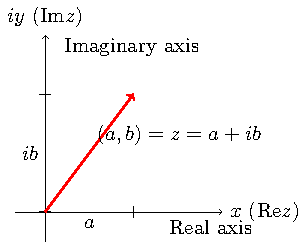
\includegraphics{complex_plane.pdf}
    % \includegraphics[width=0.8\textwidth]{figures/graph.pdf}
    % \caption{My compiled graph}
    % \label{fig:mygraph}
% \end{figure}

$x$ $(\Re z)$ Real Axis

The plane $(x,y)$ is called the complex plane. The $x$-axis is called the real axis and the $y$-axis is called the imaginary axis.

% \begin{figure}[h]
%     \centering
    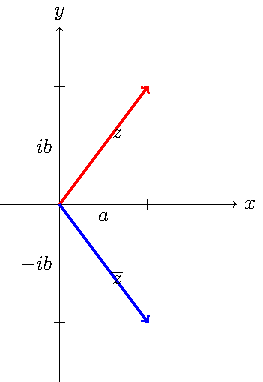
\includegraphics{complex_conjugate.pdf}
% \end{figure}

The complex conjugate of $z$ in this plane is described by a vector that is symmetric with respect to the real axis.

The sum of 2 complex numbers can be described as a sum of two vectors that start at the origin: the diagonal of the parallelogram that is constructed out of those 2 vectors.

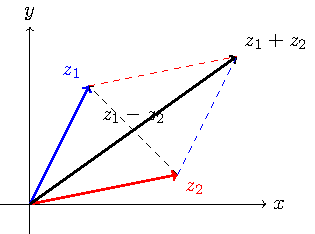
\includegraphics{sum_complex.pdf}

The difference between 2 complex numbers is the second(shorter) diagonal of the same parallelogram.
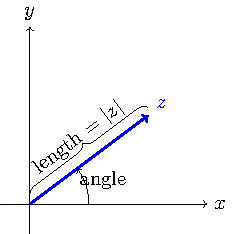
\includegraphics{length_angle_complex.pdf}

Recall: any vector is uniquely determined by its length and the angle that it creates with the $x$-axis [in the counterclockwise, positive direction]

\begin{definition}[Alternative]
 The distance from the origin $(0,0)$ to the point $z = (x,y)$ is called the modulus of the complex number $z$.
\end{definition}
Let us assume that this is the only definition and obtain previous definition from it.
By the Pythagorean theorem we get:
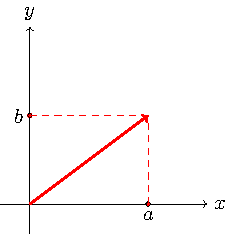
\includegraphics{coordinates_complex.pdf}

$\lvert z\rvert = \sqrt{a^2+b^2}(= \lvert a+ib \rvert)$. This is exactly the previous modulus definition.

\begin{example}
Compute $\lvert z\rvert$ for $z_1=7+9i$, $z_2=4-3i$.
$\lvert z_1\rvert = \lvert 7+9i\rvert = \sqrt{7^2+9^2} = \sqrt{130}$
$\lvert z_2\rvert = \lvert 4-3i\rvert = \sqrt{4^2+(-3)^2} = \sqrt{25} = 5$

Check (very easy!): The distance between any two points
$z=(x,y)$ and $z_0=(x_0,y_0)$ is
\[ \lvert z-z_0\rvert = \lvert (x-x_0)+i(y-y_0)\rvert = \sqrt{(x-x_0)^2+(y-y_0)^2} \]
\end{example}

The equations $\lvert z_1 \rvert =\sqrt{130}$, $\lvert z_2 \rvert =5$ describe the geometric place of all the points $z$ that are at distance $\sqrt{130}$ or $5$ from the origin - namely, it is a circle. In general we have:
Circle with radius $R$ centered at $z_0$: $\lvert z-z_0\rvert = R$.
\begin{example}
$\lvert z+1+i\rvert = 2$: circle centered at $z_0 = -(1+i)$ of radius $2$.

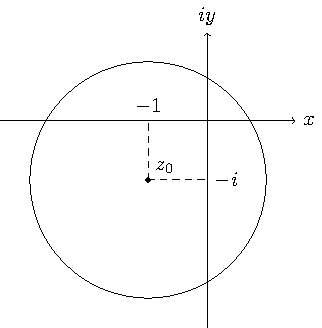
\includegraphics{circle_coord_cmplx.pdf}

Indeed, all the points for which this equation holds lie on the circle described by $\sqrt{(x+1)^2+(y+1)^2} = 2$
\end{example}

The equation $\lvert z-z_0 \rvert <R$ describes all the points that lie inside the circle centered at $z_0$ of radius $R$ (but not on the circle!). 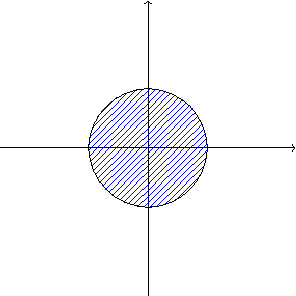
\includegraphics{filled_circle.pdf}

\begin{example}
 Find the geometric place of the points $z$ for which $\lvert z+2 \rvert - \lvert z-2\rvert = 1$
\end{example}
We are looking for the geometric place of all points $z$ such that the difference of distances from the point $z$ to two points $z=2$ and $z=-2$ is $1$. Let us show that this is a hyperbola.
Recall: hyperbola equation $\frac{x^2}{a^2} - \frac{y^2}{b^2} = 1$ - hyperbola with vertices at $(a,0)$ and $(-a,0)$ with asymptotes at $y=\pm \frac{b}{a}x$.

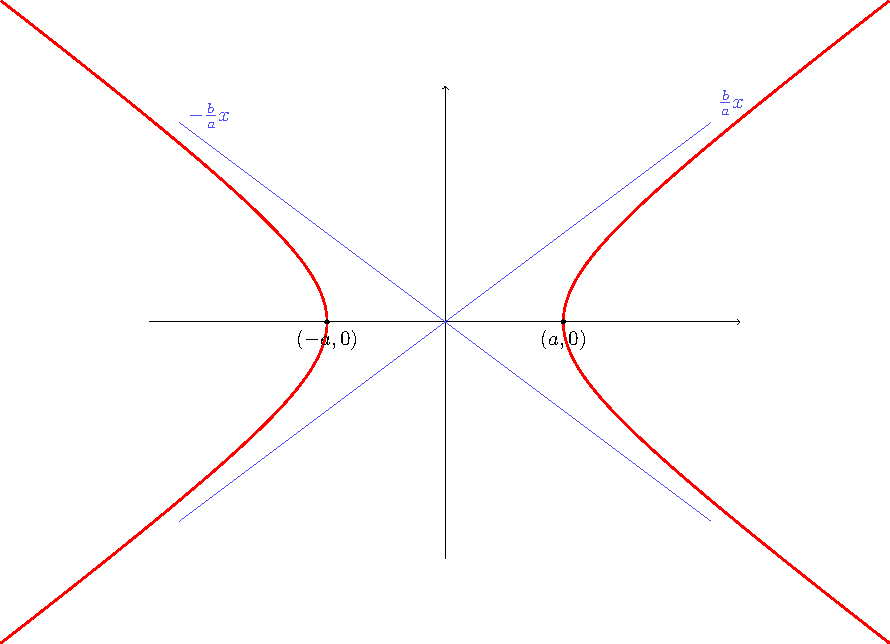
\includegraphics[width=0.7\textwidth]{hyperbola_cmplx.pdf}

For $-\frac{y^2}{b^2}+\frac{x^2}{a^2} = 1$: the vertices are at $(0,b)$ and $(0,-b)$ and asymptotes at $y=\pm \frac{b}{a}x$.

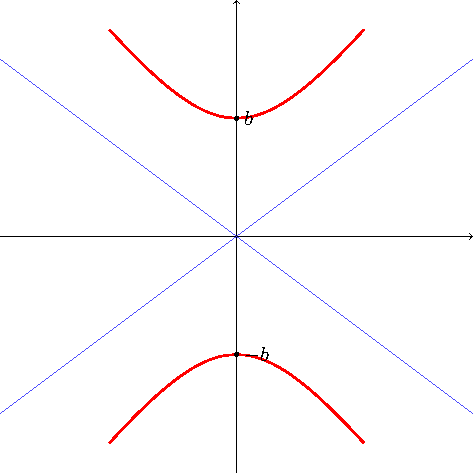
\includegraphics{hyperbola2-cmplx.pdf}

% 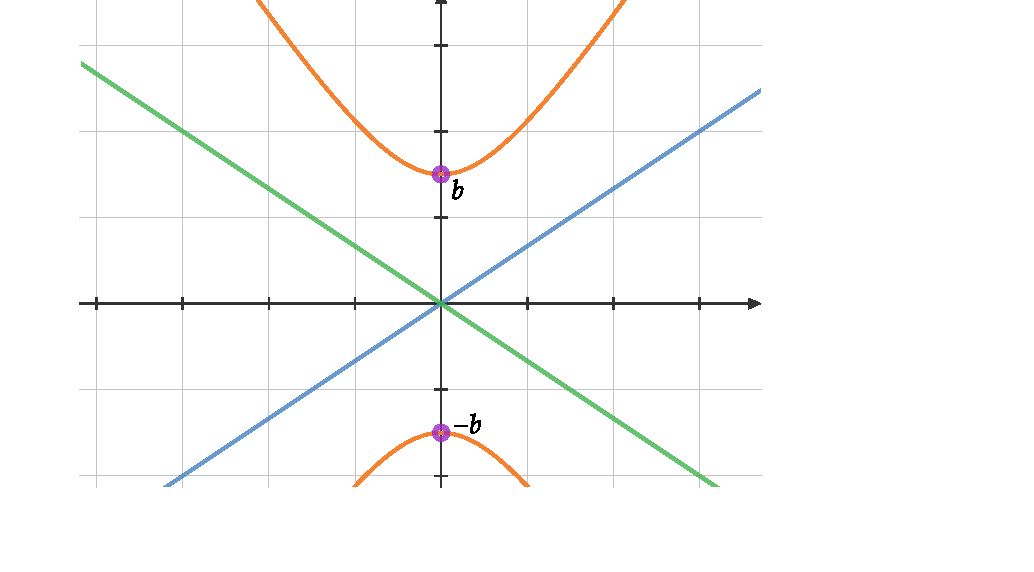
\includegraphics{hyperbola2-complex.pdf}
Here we have:
$ \lvert z+2 \rvert -\lvert z-2\rvert = 1 \implies \lvert x+iy+2\rvert - \lvert x+iy-2\rvert = 1 $
$ \implies \lvert (x+2)+iy\rvert-\lvert(x-2)+iy\rvert = 1 \implies \sqrt{(x+2)^2+y^2} - \sqrt{(x-2)^2+y^2} = 1 $
$ \implies \sqrt{(x+2)^2+y^2} = 1 + \sqrt{(x-2)^2+y^2} \iff (x+2)^2+y^2 = 1 + (x-2)^2+y^2 + 2\sqrt{(x-2)^2+y^2} $
$ \iff (x+2)^2 - (x-2)^2 -1 = 2\sqrt{(x-2)^2+y^2} \iff x^2+4x+4-x^2+4x-4-1 = 2\sqrt{(x-2)^2+y^2} $
$ \iff 8x-1 = 2\sqrt{(x-2)^2+y^2} \iff (8x-1)^2 = 4((x-2)^2+y^2) $
$ \iff 64x^2-16x+1 = 4x^2-16x+16+4y^2 \implies 60x^2-4y^2 = 15$
$ \iff 4x^2 - \frac{y^2}{15/4} = 1 \iff \frac{x^2}{1/4} - \frac{y^2}{15/4} = 1 \iff \frac{x^2}{(1/2)^2} - \frac{y^2}{(\sqrt{15}/2)^2} = 1 $
Thus, this is a hyperbola with vertices at $(\pm \frac{1}{2}, 0)$ with asymptotes $y= \pm\frac{\sqrt{15}/2}{1/2}x = \pm \sqrt{15}x$

Now we define the second object needed for a unique definition of a vector - an angle. This angle is called the argument of a complex number.

\begin{definition}
An \emph{argument} of $z \neq 0$, denoted by $\arg z$, is an angle $\theta$ such that $\cos\theta = \frac{\Re z}{\lvert z\rvert}$, $\sin \theta = \frac{\Im z}{\lvert z\rvert}$.
\end{definition}
 It is only defined up to the addition of multiples of $2\pi$. We say that $\theta$ is the \emph{principle value} of the argument if $0\leq \theta < 2\pi$ and denote the principal value of the argument $z$ by $\text{Arg} z$.

 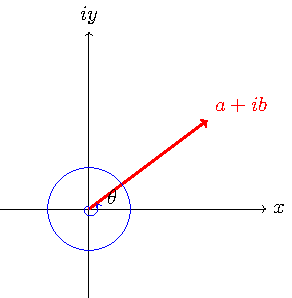
\includegraphics{angle_complex.pdf}
 
 The argument is exactly the angle that the vector $z$ creates with the $x$-axis when measured following the positive (anti-clockwise) direction.
 As we said: the argument takes infinitely many values that differ one from another by a multiple of $2\pi$.
 So, now we have 3 ways to represent a complex number: as an ordered pair, an algebraic form $x+iy$, or via its modulus and an argument.
 Representation: $z=(x,y), z=x+iy$, or $x= \lvert z\rvert\cos\theta, y=\lvert z\rvert\sin\theta \implies z=\lvert z\rvert(\cos\theta + i\sin\theta)$ Polar form ($r,\theta$ - coordinates.)
 The last form is called the polar form of a complex number.

It is more convenient to use the algebraic form to add complex numbers and it is easier to multiply using the polar form. Let us see how we pass from an algebraic to polar representation.

\begin{example}
 Write the following numbers in polar form:
 \begin{enumerate}[label=(\alph*)]
    \item $-2+2i$ 
    \item $2$ 
    \item $-i$
\end{enumerate}
    \begin{soln}
\begin{enumerate}[label=\alph*)]
    \item $z=-2+2i \implies \lvert z\rvert = \sqrt{(-2)^2+2^2} = 2\sqrt{2}$, $\cos\theta = \frac{-2}{2\sqrt{2}} = -\frac{1}{\sqrt{2}}$, $\sin\theta = \frac{2}{2\sqrt{2}} = \frac{1}{\sqrt{2}} \implies \theta = \frac{3\pi}{4}(+2\pi k, k\in \mathbb{Z}) \implies z = 2\sqrt{2}(\cos\frac{3\pi}{4}+i\sin\frac{3\pi}{4})$
    \item $z=2 \implies \lvert z\rvert = \sqrt{2^2+0^2} = 2$, $\cos \theta = \frac{2}{2} = 1$, $\sin\theta = \frac{0}{2} = 0 \implies \theta = 0(+2\pi k, k\in \mathbb{Z}), z=2(\cos 0 + i\sin 0)$
    \item $z=-i \implies \lvert z\rvert = \sqrt{0^2+(-1)^2} = 1$, $\cos\theta = \frac{0}{1} = 0$, $\sin\theta = \frac{-1}{1}=-1 \implies \theta = \frac{3\pi}{2}(+2\pi k, k\in \mathbb{Z}) \implies z = 1(\cos(\frac{3\pi}{2})+i\sin(\frac{3\pi}{2}))$
\end{enumerate}
    \end{soln}
\end{example}

 In all previous examples the argument is up to the addition of $2\pi k$.
 \begin{remark}
$a \equiv b(\text{mod } c)$: means that there exists an integer $k\in\mathbb{Z}$ s.t. $a-b=kc$.
In particular, if $c=2\pi$, then $a\equiv b(\text{mod } 2\pi)$ means that there exists $k \in \mathbb{Z}$ s.t. $a-b=2\pi k$.
\textbf{Important}: The argument of $z=0$ is not defined!
 \end{remark}
We have already studied some of the properties of the modulus in proposition~\ref{proposition:1.2}.

\begin{proposition}\label{proposition:1.2.5}
For any $z_1, z_2 \in \mathbb{C} (z_2\neq 0)$.
\begin{enumerate}
    \item $\lvert \bar{z}\rvert =\lvert z\rvert$
    \item $z\bar{z}=\lvert z\rvert^2$
    \item $\lvert \frac{z_1}{z_2} \rvert = \frac{ \lvert z_1 \rvert } { \lvert z_2 \rvert } $
\end{enumerate}
\end{proposition}
\begin{proof}    
    Here we present the proof of 1) via polar coordinates; 
    \verifythis the rest including the ones from proposition~\ref{proposition:1.2} (in the same way).
    Let $z = \lvert z\rvert(\cos\theta + i\sin\theta)$.
    $\bar{z} = \lvert z\rvert(\cos\theta - i\sin\theta)$
    $\lvert z\rvert = \lvert z\rvert\sqrt{\cos^2\theta + \sin^2\theta} = \lvert z\rvert$
    $\lvert \bar{z}\rvert = \lvert z\rvert\sqrt{\cos^2\theta + (-\sin\theta)^2} = \lvert z\rvert\sqrt{\cos^2\theta+\sin^2\theta} = \lvert z\rvert$
\end{proof}

Let us study the properties of the argument.
\begin{proposition}\label{proposition:1.3}
For any $z_1, z_2 \in \mathbb{C}(z_1, z_2 \neq 0)$
\begin{enumerate}
    \item $\arg(z_1z_2) = \arg z_1+\arg z_2$
    \item $\arg(\frac{z_1}{z_2}) = \arg z_1 - \arg z_2$
\end{enumerate}
\end{proposition}
Here we prove 1). Prove 2) in the same way.

\begin{proof}
Write $z_1,z_2$ in polar form: let $r_1 = \lvert z_1 \rvert $, $r_2 = \lvert z_2 \rvert $, $\phi_1 = \arg z_1$, $\phi_2 = \arg z_2$. Then $z_1 = r_1(\cos\phi_1+i\sin\phi_1)$ ,$z_2 = r_2(\cos\phi_2+i\sin\phi_2)$

$z_1/z_2 = r_1/r_2 (\cos\phi_1/\cos\phi_2 + i \sin\phi_1/\sin\phi_2)$
(4) $z_1z_2 = r_1r_2(\cos\phi_1\cos\phi_2 - \sin\phi_1\sin\phi_2+i(\sin\phi_1\cos\phi_2+\sin\phi_2\cos\phi_1)) = r_1r_2
= r_1r_2(\cos(\phi_1+\phi_2) + i\sin(\phi_1+\phi_2))$

Since $\arg z_1 = \phi_1 + 2\pi k$, $\arg z_2 = \phi_2 + 2\pi m \implies \arg(z_1z_2) = \phi_1 + \phi_2 + 2\pi n$, where $n = m + k$  (1)

\end{proof}

\begin{exercise}
    \begin{enumerate}
        \item $\implies$ The Geometric rule for multiplication: multiply moduli, add arguments.
        
        From rule: If $z_1 = z_2 = z$, from (4): $z^2 = r^2(\cos 2\phi + i\sin 2\phi)$.
        It is easy to prove by induction on $n$:
        \textbf{De Moivre formula} $z^n = \lvert z\rvert^n(\cos(n\phi) + i\sin(n\phi))$ \label{formula:De.Moivre}
    \end{enumerate}
\end{exercise}

\begin{example}
Express $\cos 3\alpha$ and $\sin 3\alpha$ in terms of $\cos\alpha$, $\sin\alpha$.

\begin{soln}  Construct complex number $z = \cos\alpha + i\sin\alpha$. By De Moivre formula $z^3 = \cos 3\alpha + i\sin 3\alpha$. On the other hand:
$z^3 = (\cos\alpha + i\sin\alpha)^3 = \cos^3\alpha + 3i\cos^2\alpha\sin\alpha + 3i^2\cos\alpha\sin^2\alpha + i^3\sin^3\alpha = \cos^3\alpha - 3\cos\alpha\sin^2\alpha + i(3\cos^2\alpha\sin\alpha - \sin^3\alpha)$

By the equality definition: $z_1=z_2 \iff \Re(z_1) = \Re(z_2)$ and $\Im(z_1) = \Im(z_2)$.
Let us compare these two expressions:
$\cos 3\alpha + i\sin 3\alpha = \cos^3\alpha - 3\cos\alpha\sin^2\alpha + i(3\cos^2\alpha\sin\alpha - \sin^3\alpha)$
$\implies \cos 3\alpha = \cos^3\alpha - 3\cos\alpha\sin^2\alpha$
$\sin 3\alpha = 3\cos^2\alpha\sin\alpha - \sin^3\alpha$
\end{soln}
\end{example}

\begin{example}
Define $\frac{1}{z}$ geometrically.

\begin{soln}  Let us compute the modulus and the argument.
By proposition~\ref{proposition:1.2.5} part 3): $\lvert \frac{1}{z}\rvert = \frac{1}{\lvert z\rvert}$ and since $z\cdot \frac{1}{z} = 1$
$0 = \arg 1 = \arg(z\cdot \frac{1}{z}) = \arg z + \arg \frac{1}{z} \implies \arg \frac{1}{z} = -\arg z$
\end{soln}
\end{example}

\subsection{Roots and Euler's formula}

\begin{definition}
$n$-th root of a complex number $z$ is a complex number $w$ such that $z = w^n$ (Notation: $\sqrt[n]{z} = w$)
\end{definition}

\begin{example}
Find the formula for computing roots of a given $z \in \mathbb{C}$.

\begin{soln}  Let $z=w^n$, let us write $z$ and $w$ in polar form.
$z = r(\cos\psi + i\sin\psi)$
$w = \rho(\cos\theta + i\sin\theta)$

Now we express $\rho$ and $\theta$ in terms of $r$ and $\psi$ ($r, \psi$ are given!).
From the definition: $z=w^n$ or $r(\cos\psi + i\sin\psi) = \rho^n(\cos(n\theta) + i\sin(n\theta))$
$\implies \rho^n = r$, $\cos(n\theta) = \cos\psi$, $\sin(n\theta) = \sin\psi \implies \rho = \sqrt[n]{r}$, $\theta = \frac{\psi + 2\pi k}{n}$ for $0\leq k \leq n-1$.
It is easy to see (check!) that for $k>n-1$ we will get again the same values!. Thus, we obtain
\begin{equation}\label{equation:244.1}
    w = \sqrt[n]{r}(\cos(\frac{\psi + 2\pi k}{n}) + i\sin(\frac{\psi + 2\pi k}{n})), \quad k=0,1,2,\ldots,n-1. \tag{**}
\end{equation}
\end{soln}
\end{example}

\begin{corollary}
$n$-th root of a complex number takes exactly $n$ different values that are placed on the vertices of a regular polygon with $n$ sides inscribed in a circle centered at 0 of radius $\sqrt[n]{\lvert z\rvert}$.
\end{corollary}

Recall: regular polygon is a polygon whose sides and angles are equal.

\begin{example}
Compute $\sqrt[4]{1-i}$.

\begin{soln}  We need to compute the modulus and the argument of 1-i.
$\lvert 1-i\rvert = \sqrt{1^2+(-1)^2} = \sqrt{2}$, $\cos\theta = \frac{1}{\sqrt{2}}$, $\sin\theta = \frac{-1}{\sqrt{2}} \implies \theta = \frac{7\pi}{4} + 2\pi k$ (or $\theta = -\frac{\pi}{4} + 2\pi k$)
$\implies 1-i = \sqrt{2}(\cos\frac{7\pi}{4} + i\sin\frac{7\pi}{4})$ - the polar form of 1-i.

Using formula (\ref{equation:244.1}) we get
$w = \sqrt[n]{1-i} = 2^{1/8}(\cos(\frac{7\pi/4 + 2\pi k}{4}) + i\sin(\frac{7\pi/4 + 2\pi k}{4}))$, $k=0,1,2,3$
$k=0: \quad 2^{1/8}(\cos\frac{7\pi}{16} + i\sin\frac{7\pi}{16}) \approx 0.21 + i1.07$
$k=1: \quad 2^{1/8}(\cos\frac{15\pi}{16} + i\sin\frac{15\pi}{16}) \approx -1.07 + i0.21$
$k=2: \quad 2^{1/8}(\cos\frac{23\pi}{16} + i\sin\frac{23\pi}{16}) \approx -0.21 - i1.07$
$k=3: \quad 2^{1/8}(\cos\frac{31\pi}{16} + i\sin\frac{31\pi}{16}) \approx 1.07 - i0.21$

Let us draw these roots on a circle, centered at $0$ of radius $2^{1/8}$. Connecting the neighboring roots we obtain a square.

\end{soln}
\end{example}

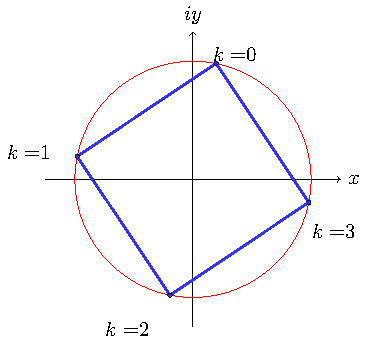
\includegraphics{circle_square.pdf}


\begin{example}
Compute all the roots of $z = \sqrt[4]{-4}$.

\begin{soln}  $\lvert -4\rvert = 4$, $\cos\theta = \frac{-4}{4} = -1$, $\sin\theta = \frac{0}{4} = 0 \implies \theta = \pi + 2\pi k$
From (\ref{equation:244.1}) we get
$\sqrt[4]{-4} = 4^{1/4}(\cos\frac{\pi + 2\pi k}{4} + i\sin\frac{\pi + 2\pi k}{4}) = \sqrt{2}(\cos(\frac{\pi}{4} + \frac{\pi k}{2}) + i\sin(\frac{\pi}{4} + \frac{\pi k}{2}))$ for $k=0,1,2,3$.
$k=0: \quad \sqrt{2}(\cos\frac{\pi}{4} + i\sin\frac{\pi}{4}) = \sqrt{2}(\frac{1}{\sqrt{2}} + i\frac{1}{\sqrt{2}}) = 1+i$
$k=1: \quad \sqrt{2}(\cos\frac{3\pi}{4} + i\sin\frac{3\pi}{4}) = \sqrt{2}(-\frac{1}{\sqrt{2}} + i\frac{1}{\sqrt{2}}) = -1+i$
$k=2: \quad \sqrt{2}(\cos\frac{5\pi}{4} + i\sin\frac{5\pi}{4}) = \sqrt{2}(-\frac{1}{\sqrt{2}} - i\frac{1}{\sqrt{2}}) = -1-i$
$k=3: \quad \sqrt{2}(\cos\frac{7\pi}{4} + i\sin\frac{7\pi}{4}) = \sqrt{2}(\frac{1}{\sqrt{2}} - i\frac{1}{\sqrt{2}}) = 1-i$

%\begin{wrapfigure}[]{r}{0.5\textwidth}
%    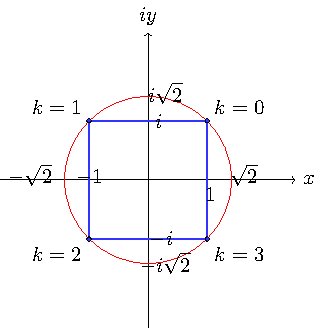
\includegraphics{circle_square2.pdf}
%\end{wrapfigure}

%\begin{figure}[htbp] % htbp = here, top, bottom, page (placement preference)
%    \centering
    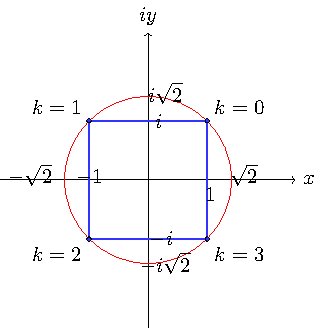
\includegraphics[width=0.5\textwidth]{circle_square2.pdf}
    % \caption{Optional: Roots of $z=\sqrt[4]{-4}$} % Add caption if needed
    % \label{fig:circle_square2} % Add label if needed
%\end{figure}
\end{soln}
\end{example}

The following formula is one of the most celebrated formulas in mathematics.

\begin{theorem}[Euler's formula; Euler 1760]\label{theorem:1.1}
Let $\theta \in \mathbb{R}$. Then $\cos\theta + i\sin\theta = e^{i\theta}$ where $e^{i\theta}$ denotes the sum of the power series $e^{i\theta} = 1 + i\theta + \frac{(i\theta)^2}{2!} + \frac{(i\theta)^3}{3!} + ... = \sum_{n=0}^{\infty}\frac{(i\theta)^n}{n!}$.
\end{theorem}

Set $\theta = \pi$. From this formula: $e^{i\pi} = -1$ - we have connected $-1$, $e$, $i$, $\pi$ in one formula!

We cannot prove this theorem now: first, we will need to examine the properties of the power series, however, we shall use it as a convenient notation even before we proved it. From the formula:
$\Re e^{i\theta} = 1 - \frac{\theta^2}{2!} + \frac{\theta^4}{4!} - ... = $ The Taylor series for $\cos\theta$ (about $\theta = 0$)
$\Im e^{i\theta} = \theta - \frac{\theta^3}{3!} + \frac{\theta^5}{5!} - ... = $ The Taylor series for $\sin\theta$ (about $\theta = 0$)

This formula provides a way of conversion between Cartesian coordinates $x+iy$ and the polar form (modulus and argument) as follows:
If $z\neq 0$: $\lvert z\rvert=r$, $\arg z = \theta \implies z = re^{i\theta}$ (the polar form)

Then $\bar{z} = x-iy = r(\cos\theta - i\sin\theta) = re^{-i\theta}$.
The following should be true:
$e^{i\theta} = e^{i(\theta + 2\pi n)}$ for every $n\in\mathbb{Z}$ (Euler's formula)
$e^{i(\phi + \psi)} = e^{i\phi}e^{i\psi}$
$\frac{1}{e^{i\theta}} = e^{-i\theta}$
$(e^{i\theta})^n = e^{in\theta}$ for every $n\in\mathbb{Z}$.

These facts are easily proved using theorem~\ref{theorem:1.1}, but they are not obvious, 
since $e^{i\theta}$ means $1 + i\theta + \frac{(i\theta)^2}{2!} + ...$ and raising the real 
number $e$ to the purely imaginary power $i\theta$ is not well-defined at the moment.
%\usepackage{xr}

% \externaldocument{note01}
% \externaldocument{note02}
% \externaldocument{note03}
% \externaldocument{note04}
% \externaldocument{note05}
% \externaldocument{note06}
% \externaldocument{note07}
% \externaldocument{note08}
% \externaldocument{note09}
% \externaldocument{note10}
% \externaldocument{note11}

\graphicspath{./input/graphs/note02/}


\zexternaldocument{note01}
\zexternaldocument{note02}
\zexternaldocument{note03}
\zexternaldocument{note04}
\zexternaldocument{note05}
\zexternaldocument{note06}
\zexternaldocument{note07}
\zexternaldocument{note08}
\zexternaldocument{note09}
\zexternaldocument{note10}
\zexternaldocument{note11}
% \externaldocument{note12}



% \section*{Week 2}
\week{2}
% \subsection*{Lecture 4}
\lecture{4}{Functions of a Complex Variable}

In this lecture we shall discuss the basic properties of functions of one complex variable.

\section{Functions of a Complex Variable}

\begin{definition}\label{definition:2.1}
     Let $S \subseteq \mathbb{C}$ be a subset of complex numbers. A function $f$ on $S$ is a rule which assigns to each $z \in S$ a complex number (or complex numbers) $f(z)$, 
    called the value of $f$ at $z$. $S$ is called the Domain of Definition (DoD).
\end{definition}
\begin{definition} \label{definition:2.2}
     If for every $z$ in the DoD corresponds one value $w$, then we say that $f$ is a single-valued function. If to $z$ correspond several values, then $f$ is a multi-valued function.
\end{definition}
\begin{example} \label{example:3.1}
     $f(z) = \frac{1}{z}$: $f$ is not defined at $z = 0$ and it is defined and single-valued everywhere else.
\end{example}
For example, the value of $f$ at $z = 8 - 3i$ is
\[ f(8 - 3i) = \frac{1}{8 - 3i} = \frac{1}{8 - 3i} \cdot \frac{8 + 3i}{8 + 3i} = \frac{8 + 3i}{8^2 + 3^2} = \frac{8 + 3i}{73} = \frac{8}{73} + i\frac{3}{73}\]

\begin{example}\label{example:3.2}
     $f(z) = \sqrt{z + 1}$ defined everywhere on $\mathbb{C}$ and it is double-valued function: $f(0) = 1$ and $f(0) = -1$ (for instance).
\begin{align*}
    & f(0) = \sqrt{1}: \vert 1\vert  = 1, \quad \cos \theta = \frac{1}{1} = 1, \quad \sin \theta = \frac{0}{1} = 0 \implies \theta = 0 + 2\pi k \\
    & \implies \sqrt{1} = \cos\left(\frac{0 + 2\pi k}{2}\right) + i\sin\left(\frac{2\pi k}{2}\right), \quad k = 0, 1 \\
    & k = 0: \cos 0 + i\sin 0 = 1, \quad k = 1: \cos \pi + i\sin \pi = -1 \\
\end{align*}
\end{example}
\begin{example}\label{example:3.3}
     $f(z) = \sqrt{z - 1} + \sqrt{z + 1}$ is 4-valued: for example, if $z = 0$, we get $w_1 = i + 1, w_2 = -i + 1, w_3 = i - 1, w_4 = -i - 1$ (\verifythis)
\end{example}
\begin{example} \label{example:3.4}
     Polynomials. General form: $P_n(z) = \sum_{j=0}^{n} a_j z^j$ - polynomial of degree $n$ of complex variable $z$ with complex coefficients $a_j \in \mathbb{C}$.
\end{example}
For example: $f(z) = z^2, f(z) = 4 + iz - z^2 + (1 + i)z^3$.

\begin{example}\label{example:3.5}
    Rational function \{ratio of two polynomials\}. General form:
\[f(z) = \frac{a_0 + a_1 z + \dots + a_n z^n}{b_0 + b_1 z + \dots + b_m z^m}\]
defined and single-valued everywhere, except for the roots (zeros) of the denominator.
\end{example}
\begin{example} \label{example:3.6} The exponential function $f(z) = e^z$.

Defined to be the series $e^z = \sum_{n=0}^{\infty} \frac{z^n}{n!} = 1 + \frac{z}{1!} + \frac{z^2}{2!} + \dots$ or equally well by Euler's formula: $e^z = e^x(\cos y + i\sin y)$ \{for $z = x + iy$\}.
\end{example}
We will see later that the above series converges absolutely for all $z \in \mathbb{C}$, thus $f(z) = e^z$ can be defined for every $z$ in $\mathbb{C}$, namely, we can take the DoD to be $\mathbb{C}$. 
It is single-valued.


\begin{example} \label{example:3.7}
     Trigonometric and Hyperbolic functions. For $z \in \mathbb{C}$ define:
\begin{equation} \cos z = \frac{1}{2}(e^{iz} + e^{-iz}), \quad \sin z = \frac{1}{2i}(e^{iz} - e^{-iz}) \tag{*}\end{equation}
which agrees with the definition for real $z$ (by Euler's formula). By analogy with the real case, we define
\begin{equation} \cosh z = \frac{1}{2}(e^z + e^{-z}), \quad \sinh z = \frac{1}{2}(e^z - e^{-z})\tag{**}\end{equation}
Using (*) and (**) it is easy to check that \checkthis $\cos z + i\sin z = e^{iz} = \cosh(iz) + \sinh(iz)$.
\end{example}
Let $z = x + iy$. We rewrite $f(z)$ and separate its real and imaginary parts as follows:
(1) $f(z) = \text{Re } f(z) + i\text{Im } f(z) = u(x, y) + iv(x, y)$.

In this way we can think of $f$ as of a real mapping:
$f: \mathbb{R}^2 \to \mathbb{R}^2$: (2) $(x, y) \mapsto (u(x, y), v(x, y)) \quad u, v: \mathbb{R}^2 \to \mathbb{R}$.

Let $z = r(\cos \theta + i\sin \theta)$ \{the polar form\}. Then, in a similar way $f: \mathbb{R}^2 \to \mathbb{R}^2$: (3) $f(r, \theta) = \phi(r, \theta) + i\psi(r, \theta)$.

\begin{example} \label{example:3.8}
     Write in the form (1) or (3)
a) $f(z) = z^2$ b) $f(z) = \vert z\vert $ c) $f(z) = \text{Re } z$ d) $f(z) = z^n$ e) $f(z) = e^z$.

\begin{soln} a) Denote $z = x + iy$. Then $z^2 = (x + iy)^2 = (x^2 - y^2) + i2xy \implies \text{Re } z^2 = x^2 - y^2, \text{Im } z^2 = 2xy$, and $f(x, y) = (x^2 - y^2, 2xy)$.
OR: $z = r(\cos \theta + i\sin \theta) \implies z^2 = r^2(\cos 2\theta + i\sin 2\theta)$, where $r = \vert z\vert $, thus $\text{Re } z^2 = r^2 \cos 2\theta, \text{Im } z^2 = r^2 \sin 2\theta$, and $f(r, \theta) = (r^2 \cos 2\theta, r^2 \sin 2\theta)$.

b) $\vert z\vert  = \vert x + iy\vert  = \sqrt{x^2 + y^2} \implies f(x, y) = (\sqrt{x^2 + y^2}, 0) = \sqrt{x^2 + y^2} \to$ real function!

c) $z = x + iy, \text{Re } z = x \implies f(x, y) = (x, 0) = x \to$ real function!
$z = x + iy, \text{Im } z = y \implies$ for $f(z) = \text{Im } z: f(x, y) = (y, 0) = y \to$ real!

d) Let $z = r(\cos \theta + i\sin \theta)$ \{$r = \vert z\vert $\}. Then, by De Moivre formula $z^n = r^n(\cos(n\theta) + i\sin(n\theta))$, and $f(r, \theta) = (r^n \cos(n\theta), r^n \sin(n\theta))$.

e) Let $z = x + iy$. Then, by Euler's formula: $e^z = e^x(\cos y + i\sin y) \implies f(x, y) = (e^x \cos y, e^x \sin y)$.
\end{soln}
\end{example}
We can also do the opposite: given a function of $x, y$ we can rewrite it in terms of $z$ and its conjugate:
Recall: $\text{Re } z = \frac{1}{2}(z + \bar{z}), \text{Im } z = \frac{1}{2i}(z - \bar{z})$.

\begin{example} \label{example:3.9} Rewrite in terms $z$ and $\bar{z}$:
a) $f(x, y) = x^2 - y + i(x + y^2)$ b) $f(x, y) = x^2 - 1$.

\begin{soln} a)
\begin{align*}
x^2 - y + i(x + y^2) &= \left(\frac{z + \bar{z}}{2}\right)^2 - \frac{z - \bar{z}}{2i} + i\left(\frac{z + \bar{z}}{2} + \left(\frac{z - \bar{z}}{2i}\right)^2\right) \\
&= \frac{1}{4}(z^2 + 2z\bar{z} + \bar{z}^2) - \frac{1}{2i}(z - \bar{z}) + i\left(\frac{1}{2}(z + \bar{z}) + \frac{1}{4i^2}(z^2 - 2z\bar{z} + \bar{z}^2)\right) \\
&= \frac{1}{4}(z^2 + 2z\bar{z} + \bar{z}^2) - \frac{1}{2i}(z - \bar{z}) + \frac{i}{2}(z + \bar{z}) - \frac{i}{4}(z^2 - 2z\bar{z} + \bar{z}^2) \\
&= \frac{1}{4}(z^2 + 2z\bar{z} + \bar{z}^2) + \frac{i}{2}z - \frac{i}{2}\bar{z} + \frac{i}{2}z + \frac{i}{2}\bar{z} - \frac{i}{4}(z^2 - 2z\bar{z} + \bar{z}^2) \\
&= \frac{1}{4}(z^2 + \bar{z}^2)(1 - i) + \frac{1}{2}z\bar{z}(1 + i) + iz
\end{align*}

b) $x^2 - 1 = \frac{1}{4}(z^2 + \bar{z}^2 + 2z\bar{z}) - 1 = \frac{1}{4}(z^2 + \bar{z}^2 + 2z\bar{z} - 4)$.
\end{soln}

\end{example}
\subsection{Transformations of the Complex plane}

A complex function is a map (transformation) from $\mathbb{C}$ to $\mathbb{C}$, but to draw a graph of such mapping we would need $2 + 2 = 4$ real dimensions.

Instead, we shall examine what happens to various shapes - lines, circles, etc, under such map. Let us assume that $f$ is single-valued function defined on some domain of definition. 
We will treat the function as a map that maps a set from $(x, y)$-plane to some other set in $(u, v)$-plane. Let us start with two simple examples.

\begin{example} \label{example:4.1} 
    Let $f(z) = \text{Im } z$ (defined and single-valued everywhere). Let us find its image \{namely, where to the complex plane $\mathbb{C}$ is mapped\}.
$\text{Im } z = y \in \mathbb{R} \implies$ the complex plane $\mathbb{C}$ is mapped to $\mathbb{R}$.

\includegraphics{image_lin.pdf}
\end{example}
\begin{example} \label{example:4.2} What is the image of the ray $\arg z = \frac{\pi}{3}$ under $f(z) = z^3$?

\begin{soln} Let us write the function $f$ in polar coordinates.
$f(z) = r^3(\cos \theta + i\sin \theta)^3 = r^3(\cos 3\theta + i\sin 3\theta)$ \{$r = \vert z\vert $\} De Moivre.
\end{soln}

\end{example}
Thus, the image of $\arg z = \frac{\pi}{3}$ under $z^3$ is $r^3(\cos(3 \cdot \frac{\pi}{3}) + i\sin(3 \cdot \frac{\pi}{3})) = -r^3 (r \geq 0!)$.

Recall that $r = \vert z\vert $, therefore $r \geq 0$ always. Hence, the image of that ray is the negative half of the real axis.

\includegraphics{image_lin2.pdf}

$f(z) = z^2$.

Now we will examine the mapping $f(z) = z^2$ and will find the image of various curves and shapes under this mapping. Let us rewrite $f$ in the polar and algebraic form:
$z = x + iy: f(x, y) = u(x, y) + iv(x, y) = x^2 - y^2 + i2xy$.
$z = re^{i\theta}: f(r, \theta) = r^2 e^{2i\theta} = r^2 \cos 2\theta + ir^2 \sin 2\theta$.

\begin{example} \label{example:4.3} First, we determine what is the image of x-axis and of y-axis. The real axis $\mathbb{R}$ is mapped to the positive half of the real axis $\mathbb{R}^+$. $\mathbb{R} \to \mathbb{R}^+$. 
    To see that we represent $\mathbb{R}$ as $\mathbb{R} = \mathbb{R}^+ \cup \mathbb{R}^-$, where $\mathbb{R}^+$ ($\mathbb{R}^-$) the positive (negative) half of $\mathbb{R}$. Every point in $\mathbb{R}^+$ is of the form $re^{i0} = r \geq 0$ and every point in $\mathbb{R}^-$ is of the form $re^{i\pi} = -r \leq 0$. 
    These points are mapped by $f$ to: $r^2 e^{2 \cdot i \cdot 0} = (r)^2, r^2 e^{2 \cdot 0 \cdot i\pi} = r^2 \in \mathbb{R}^+$.
    
\includegraphics{image_lin3.pdf}
\end{example}
Now we will show (in the same way) that the imaginary axis is mapped to the negative half of the real axis: $i\mathbb{R} \xrightarrow[]{z^2} \mathbb{R}^-$.

Represent the imaginary axis $i\mathbb{R}$ as: $i\mathbb{R} = (i\mathbb{R})^+ \cup (i\mathbb{R})^-$, where $(i\mathbb{R})^+$ are points of the form $re^{i\frac{\pi}{2}} = ir (r > 0)$ and $(i\mathbb{R})^-: re^{i\frac{3\pi}{2}} = -ir$. $f$ maps these points to $r^2 e^{i2 \cdot \frac{\pi}{2}} = r^2 e^{i\pi} = -r^2 \leq 0, r^2 e^{i2 \cdot \frac{3\pi}{2}} = r^2 e^{i3\pi} = -r^2 \leq 0$.

\includegraphics{image_lin4.pdf}
\begin{claim} A quarter circle of radius $r$ centered at 0 is mapped by $z^2$ to a half circle of radius $r^2$ centered at 0.
    
\includegraphics{image_lin5.pdf}
    \begin{proof}
The quarter circle is given by points $re^{i\theta}$ where $0 \leq \theta \leq \frac{\pi}{2}$. It is mapped by $z^2$ to $r^2 e^{2i\theta}$. Since $0 \leq \theta \leq \frac{\pi}{2} \implies 0 \leq 2\theta \leq \pi$, thus we obtain a half circle of radius $r^2$ centered at 0.
    \end{proof}
\end{claim}

\begin{claim} A line $l_\theta$ passing through the origin at angle $\theta$ is mapped to a ray $l_{2\theta}$ starting at 0 making an angle $2\theta$.
\end{claim}


\includegraphics{image_lin6.pdf}
The line is parameterized by $re^{i\theta}$, where $\theta$ is fixed and $r$ may vary. The map $f(z) = z^2$ sends $r$ to $r^2$ resulting in a ray and the angle is transformed from $\theta$ to $2\theta$.

Now let us find the image of a vertical line $x = c \in \mathbb{R}$: In this case the geometric representation is more convenient. $z \to z^2: (x, y) \mapsto (x^2 - y^2, 2xy)$. Set $x = c$.

We have the following system, from which we may eliminate the variable $y$ to get an equation for a curve in $(u, v)$-plane:
\begin{align*}
u &= x^2 - y^2 = c^2 - y^2 \\
v &= 2xy = 2cy
\end{align*}
$y = \frac{v}{2c} \implies u = c^2 - \frac{v^2}{4c^2}$: this is leftward opening parabola with vertex $(c^2, 0)$, intersecting the v-axis at $(0, \pm 2c^2)$ \{Note that: if $c$ is negative, the image again is the same, namely, the image is independent of the sign of $c$\}.

% \textbf{Lectures 5+6}
\lecture{5+6}{Images under $z^2$}
We continue to examine the images under $z^2$ and other transformations.

\begin{example}\label{example:4.4} Determine which regions (if any) of the z-plane are mapped to the upper half part of the w-plane under the mapping $w = z^2$.

First, we identify: the upper half of w-plane = \{$w \in \mathbb{C} \vert  \text{Im } w \geq 0$\} $\theta = \arg w \leq \pi$: An element $z = re^{i\theta} \to w = r^2 e^{2i\theta}$ is in the upper half plane iff the argument of $w$ lies between 0 and $\pi$: $0 + 2\pi k \leq 2\theta \leq \pi + 2\pi k, k \in \mathbb{Z} \implies k\pi \leq \theta \leq \frac{\pi}{2} + k\pi$. 
Namely, $z$ must lie in the first or third quadrant in order to map to the upper half plane [Plug $k = 1, 2, 3, 4$ to see this!]

Alternatively: we could use the algebraic form $x + iy$ and get: $w = z^2 = x^2 - y^2 + i2xy \implies \text{Im } w \geq 0 \iff 2xy \geq 0 \iff x, y \geq 0$ or $x, y \leq 0$. This gives again I and III quadrant.
\end{example}
Now let us study another function and its images.
\begin{example} \label{example:4.5}
    Look at $z \to \frac{1}{z} = w$.

It is an instructive exercise to draw a picture trying to determine where to various regions of the plane are mapped.

EXERCISE: 1) Show that $w = \frac{1}{z}$ maps the interior of the unit circle in the first quadrant to the exterior of the unit circle in the fourth quadrant.

2) What is the image of the unit circle under $\frac{1}{z}$?
3) Write down how $z \to \frac{1}{z} = w$ maps the punctured plane $\mathbb{C} \setminus \{0\}$ to itself (and $\mathbb{C} \cup \{\infty\}$ to itself).
\end{example}

\begin{example}
Back to Ex 4.5.(\ref{example:4.5}) Let us study two images under $\frac{1}{z}$.
a) Find the image of the line $z = t + i(1 - t)$ under $\frac{1}{z}$.

\begin{soln} Denote: $w = u + iv, z = x + iy \implies x = t, y = (1 - t)$.
\[w = u + iv = \frac{1}{x + iy} = \frac{x - iy}{x^2 + y^2} (\text{for } z \neq 0, w \neq 0) \iff u = \frac{x}{x^2 + y^2}, v = \frac{-y}{x^2 + y^2}\]
Thus, plugging $x = t, y = 1 - t$, we obtain the following system:
\begin{align*}
& t = \frac{u}{u^2 + v^2} \\
& 1 - t = \frac{-v}{u^2 + v^2} \implies \\
& t(u^2 + v^2) = u \\
& (1 - t)(u^2 + v^2) = -v
\end{align*}
$\implies u^2 + v^2 = u - v$ (we add the equations) $\implies u^2 - u + v^2 + v = 0 \implies (u - \frac{1}{2})^2 + (v + \frac{1}{2})^2 = \frac{1}{2}$ (complete the square in $u$ and in $v$).

Namely, the map $w = \frac{1}{z}$ maps the line $z = t + i(1 - t)$ to the circle (in w-plane) centered at the point $(\frac{1}{2}, -\frac{1}{2})$ with radius $\frac{1}{\sqrt{2}}$.
\end{soln}

b) Determine how the horizontal lane $y = k$ is transformed under $w = \frac{1}{z}$.

\begin{soln} Substitute as before: $x = \frac{u}{u^2 + v^2}, y = \frac{-v}{u^2 + v^2}$. Plug $y = k$:
\begin{align*}  
                & k = \frac{-v}{u^2 + v^2} \iff ku^2 + kv^2 + v = 0 \iff (k \neq 0) u^2 + v^2 + \frac{v}{k} = 0\\ 
                & \iff u^2 + (v + \frac{1}{2k})^2 = \frac{1}{4k^2} \text{ (complete the square in } v)
\end{align*}
Namely, the line is mapped onto a circle, center of which depends on the sign of $k$, and the radius is $\frac{1}{2\vert k\vert }$.
\end{soln}
\end{example}
Now we have a feeling on geometrical description of the complex functions - we will study more transformations later.

Next subject - the limits of complex functions. The introduction of a limit will allow us to investigate what it means for the complex function $f$ to be continuous and differentiable. 
Through several explicit examples, we contrast our findings with corresponding results for real functions.

\section{Limits}

Let $f$ be a complex function. We say that $\lim_{z \to z_0} f(z) = w_0$ if when $z$ is "close" to $z_0$, $f(z)$ is "close" to $w_0$. Formally:

\begin{definition}\label{definition:3.1}  
    $\lim_{z \to z_0} f(z) = w_0$ if for any given $\epsilon > 0$, there exists $\delta = \delta(\epsilon) > 0$ such that if $0 < \vert z - z_0\vert  < \delta$, then $\vert f(z) - w_0\vert  < \epsilon$.
\end{definition}
\begin{example}  Let $f(z) = \frac{z}{\bar{z}}$. Claim: for any $z_0$, $\lim_{z \to z_0} \frac{z}{\bar{z}} = \frac{z_0}{\bar{z_0}}$.

\begin{proof} Given $\epsilon > 0$, choose $\delta = 2\epsilon \vert z_0\vert $. Then, if $0 < \vert z - z_0\vert  < \delta$:
\begin{align*}
\left\vert \frac{z}{\bar{z}} - \frac{z_0}{\bar{z_0}}\right\vert  & = \left\vert \frac{z\bar{z_0} - z_0 \bar{z}}{\bar{z}\bar{z_0}}\right\vert  = \left\vert \frac{z\bar{z_0} + z\bar{z} - z\bar{z} - z_0\bar{z}}{\bar{z}\bar{z_0}}\right\vert  = \left\vert \frac{\bar{z}(z_0 - z) + z(\bar{z_0} - \bar{z})}{\bar{z}\bar{z_0}}\right\vert \\
& \leq \frac{\vert \bar{z}\vert \vert z_0 - z\vert  + \vert z\vert \vert \bar{z_0} - \bar{z}\vert }{\vert \bar{z}\vert \vert \bar{z_0}\vert } = \frac{\vert z_0 - z\vert }{\vert z_0\vert } + \frac{\vert z\vert }{\vert z\vert } \frac{\vert z - z_0\vert }{\vert z_0\vert } = \frac{2\vert z - z_0\vert }{\vert z_0\vert } < \frac{2\delta}{\vert z_0\vert } = \frac{2 \cdot 2\epsilon\vert z_0\vert }{\vert z_0\vert } = \epsilon \\
\end{align*}
Thus, for a given $\epsilon > 0$ we have found $\delta$ (that depends on $\epsilon$!) s.t. if $\vert z - z_0\vert  < \delta$, then $\vert f(z) - w_0\vert  = \left\vert \frac{z}{\bar{z}} - \frac{z_0}{\bar{z_0}}\right\vert  < \epsilon$ (for any $z_0$!).
\end{proof}
\end{example}

\begin{example}\label{example:5.2}
    Let $f(z) = \frac{z}{\bar{z}}, z \neq 0$. Prove that $\lim_{z \to 0} \frac{z}{\bar{z}}$ does not exist.
\end{example}

Before we proceed to the proof, let us show the following:

\begin{claim}\label{claim:3.1}
    If $\lim_{z \to z_0} f(z)$ exists, then it is unique.

\begin{proof}
 Assume $\lim_{z \to z_0} f(z) = a$ and $\lim_{z \to z_0} f(z) = b$. By Def 3.1(\ref{definition:3.1}) for any $\epsilon > 0$ there exist $\delta_1 > 0$ and $\delta_2 > 0$ such that
\begin{align*}
\text{if } 0 < \vert z - z_0\vert  < \delta_1 &\implies \vert f(z) - a\vert  < \epsilon/2 \\
\text{if } 0 < \vert z - z_0\vert  < \delta_2 &\implies \vert f(z) - b\vert  < \epsilon/2
\end{align*}
Choose $\delta < \min(\delta_1, \delta_2) \implies$ for $0 < \vert z - z_0\vert  < \delta$, $\vert f(z) - a\vert  < \epsilon/2$ and $\vert f(z) - b\vert  < \epsilon/2$. 
Thus, using triangle inequality, we obtain
\[ \vert a - b\vert  = \vert a - f(z) + f(z) - b\vert  \leq \vert a - f(z)\vert  + \vert f(z) - b\vert  < \frac{\epsilon}{2} + \frac{\epsilon}{2} = \epsilon \tag{*}\]
Since (*) holds for any $\epsilon > 0$ we obtain that $a = b$.
\end{proof}
\end{claim}
Back to Ex 5.2: we will use a common technique to show that the limit does not exist - we will show that there exist two different paths (directions) $z \to z_0$ along which we get 2 different limits.

\begin{soln}
Ex 5.2  Note: for real $z$ we have: \{namely, fix $y = 0$\}
$z = x \in \mathbb{R}: \frac{z}{\bar{z}} = \frac{x}{x} = 1 \implies \lim_{x \to 0} \frac{z}{\bar{z}} = 1$.

On the other hand, for purely imaginary $z$ we get: \{namely, fix $x = 0$\}
$z = iy \in i\mathbb{R}: \frac{z}{\bar{z}} = \frac{iy}{-iy} = -1 \implies \lim_{y \to 0} \frac{z}{\bar{z}} = -1$
$\implies$ the limit as $z \to 0$ does not exist.
\end{soln}
Note: 
\begin{remark} 8989 For any $z_0 \neq 0$, $\lim_{z \to z_0} \frac{z}{\bar{z}} = \frac{z_0}{\bar{z_0}}$. 
    \begin{proof} Given $\epsilon > 0$, choose $\delta = \frac{\epsilon}2 \vert z_0\vert $. Then
\begin{align*} &\left| \frac{\bar{z}}{\bar{z}} - \frac{\bar{z_0}}{z_0} \right| = \left| \frac{\bar{z}z_0 - \bar{z_0}z}{z z_0} \right| \\
        &= \left| \frac{\bar{z}z_0 + z\bar{z} - z\bar{z} - \bar{z_0}z}{z z_0} \right| = \left| \frac{\bar{z}(z_0 - z) + z(\bar{z} - \bar{z_0})}{z z_0} \right| \\
        & \leq \frac{|\bar{z}||z_0 - z| + |z||\bar{z} - \bar{z_0}|}{|z||z_0|} = \frac{|z||z_0 - z|}{|z||z_0|} + \frac{|z||z - z_0|}{|z||z_0|} = \frac{2|z - z_0|}{|z_0|} < \frac{2\delta}{|z_0|} = \frac{2}{|z_0|} \cdot \frac{\epsilon}{2}|z_0| = \epsilon, \\
\end{align*}
That's where our choice of $\delta$ come in,  $\delta = \frac{\epsilon}{2}|z_0|$
    \end{proof}
\end{remark}

\begin{example}\label{example:5.3}
    Show that $\lim_{z \to 0} \frac{\bar{z}^2}{z^2}$ does not exist.
\begin{soln} Here, for $z = x \in \mathbb{R}:  \frac{\bar{z}^2}{z^2} = \frac{x^2}{x^2} = 1$ and for $z=iy \in i\mathbb{R}: \frac{\bar{z}^2}{z^2} = \frac{(-iy)^2}{(iy)^2} = \frac{-y^2}{-y^2}=1$. 
    However, choosing the path $z=(1+i)t$ for $t \in \mathbb{R} \setminus \{0\}$ gives us $\frac{\bar{z}^2}{z^2}=\frac{((1-i)t)^2}{((1+i)t)^2} = \frac{(1-i)^2}{(1+i)^2} = \frac{1-2i-1}{1+2i-1}=-1$. $-1 \neq 1$ - does not agree with the value on previous two paths, 
    thus we can conclude that the original limit does not exist.
\end{soln}
\end{example}

Alternatively: Let $z = re^{i\theta}, r, \theta \in \mathbb{R}$. Then $z \to 0$ means $r \to 0$. Since $e^{i\theta} \neq 0$ for all $\theta \in \mathbb{R}$, We have: $\frac{\bar{z}^2}{z^2} = \frac{r^2 e^{-2i\theta}}{r^2 e^{2i\theta}} = e^{-4i\theta}$.
$\implies \lim_{z \to 0} \frac{\bar{z}^2}{z^2} = \lim_{r \to 0} e^{-4i\theta} = e^{-4i\theta}$. For different $\theta$-s we get different limits - namely, 
on different paths the limit does not agree $\implies$ the limit does not exist.
% \end{soln}

\begin{example}
Ex 5.3 (\ref{example:5.3}) shows that the different paths need not be the real and imaginary axes!
\end{example}

\begin{remark} 
    If $\lim_{z \to z_0} f(z) = w_0$ exists, then $f(z) \to w_0$ as $z \to z_0$ on *every* path (uniqueness of the limit!) 
    If on different paths $z \to z_0$ there are different values of the limit (or there exists a path on which the limit does not exist), then the limit $\lim_{z \to z_0} f(z)$ does not exist.
\end{remark}
Similarly to the real functions we have the following proposition for the complex functions.

\begin{proposition} \label{proposition:3.1} If $\lim_{z \to z_0} f(z) = w_0$ and $\lim_{z \to z_0} g(z) = w_1$, then
\begin{enumerate}
    \item $\lim_{z \to z_0} (f(z) + g(z)) = w_0 + w_1$
    \item $\lim_{z \to z_0} f(z) \cdot g(z) = w_0 w_1$
    \item If $w_1 \neq 0$, then $\lim_{z \to z_0} \frac{f(z)}{g(z)} = \frac{w_0}{w_1}$
\end{enumerate}

\begin{proof} EXERCISE - a very good exercise to "play" with $\epsilon$-$\delta$ definition! \end{proof}
\end{proposition}
Next proposition provides a relation between the limit of the complex function and its real and imaginary parts (that are real functions).

\begin{proposition}\label{proposition:3.2} Let $f(z) = u(x, y) + iv(x, y), z_0 = x_0 + iy_0$. Then $\lim_{z \to z_0} f(z) = u_0 + iv_0 = w_0 \iff \lim_{(x, y) \to (x_0, y_0)} u(x, y) = u_0 = \text{Re } w_0$ and $\lim_{(x, y) \to (x_0, y_0)} v(x, y) = v_0 = \text{Im } w_0$.
\end{proposition}
Note: the first limit is complex, but the last two limits are real!

\begin{proof}  $\implies$ Assume that $\lim_{z \to z_0} f(z) = u_0 + iv_0$. Let us show that $\lim_{(x, y) \to (x_0, y_0)} u(x, y) = u_0 = \text{Re } w_0$ and $\lim_{(x, y) \to (x_0, y_0)} v(x, y) = v_0 = \text{Im } w_0$.

By Def 3.1(\ref{definition:3.1}): given $\epsilon > 0$ there exists $\delta = \delta(\epsilon) > 0$ s.t. for all $z$ with $0 < \vert z - z_0\vert  < \delta$ we have $\vert f(z) - (u_0 + iv_0)\vert  < \epsilon$.

Since for any $z \in \mathbb{C}: \vert \text{Im } z\vert , \vert \text{Re } z\vert  \leq \vert \text{Re } z + i\text{Im } z\vert  = \vert z\vert $, we get:
\[ \vert v(x, y) - v_0\vert , \vert u(x, y) - u_0\vert  < \vert u(x, y) - u_0 + i(v(x, y) - v_0)\vert  = \vert u(x, y) + iv(x, y) - (u_0 + iv_0)\vert  = \vert f(z) - (u_0 + iv_0)\vert  < \epsilon\]
Thus $\vert u(x, y) - u_0\vert  < \epsilon$ and $\vert v(x, y) - v_0\vert  < \epsilon$.

\checkthis $\vert z - z_0\vert $ is the distance from $(x, y)$ to $(x_0, y_0)$ in $\mathbb{R}^2$.
$\implies \lim_{(x, y) \to (x_0, y_0)} u(x, y) = u_0$ and $\lim_{(x, y) \to (x_0, y_0)} v(x, y) = v_0$.

Note: $\vert z - z_0\vert  < \delta \implies \vert x + iy - (x_0 + iy_0)\vert  = \vert (x - x_0) + i(y - y_0)\vert  < \delta$, and we get $\vert x - x_0\vert , \vert y - y_0\vert  \leq \vert (x - x_0) + i(y - y_0)\vert  < \delta$.

$\impliedby$ Assume that $\lim_{(x,y) \to (x_0, y_0)} u(x, y) = u_0$ and $\lim_{(x, y) \to (x_0, y_0)} v(x, y) = v_0$.

Let $\epsilon > 0$. Since $u$ and $v$ have real limits $u_0, v_0$ as $(x, y) \to (x_0, y_0)$ from Def 3.1(\ref{definition:3.1}) there exist $\delta_1 > 0$ and $\delta_2 > 0$ such that if $0 < \vert \vert (x, y) - (x_0, y_0)\vert \vert  < \delta_1$, then $\vert u(x, y) - u_0\vert  < \epsilon/2$, and $0 < \vert \vert (x, y) - (x_0, y_0)\vert \vert  < \delta_2$, then $\vert v(x, y) - v_0\vert  < \epsilon/2$.

Choose $\delta < \min(\delta_1, \delta_2)$. Then, whenever $0 < \vert \vert (x, y) - (x_0, y_0)\vert \vert  < \delta$:
\begin{align*} 
    \vert u(x, y) + iv(x, y) - (u_0 + iv_0)\vert  &= \vert u(x, y) - u_0 + i(v(x, y) - v_0)\vert  \\ 
    & \leq \vert u(x, y) - u_0\vert  + \vert v(x, y) - v_0\vert  < \frac{\epsilon}{2} + \frac{\epsilon}{2} = \epsilon
\end{align*}
by triangle inequality.

Namely, for any $\epsilon > 0$ we have found $\delta > 0$ such that whenever $0 < \vert z - z_0\vert  < \delta: \vert f(z) - (u_0 + iv_0)\vert  < \epsilon$, as required.
\end{proof}
\week{3}
\lecture{7}{Continuation from prev.}
% \section*{Week 3 Lecture 7}
We have proved:
\[ \lim_{z \to z_0} f(z) = u_0 + iv_0 \iff \lim_{(x,y) \to (x_0, y_0)} u(x,y) = u_0 \text{ and } \lim_{(x,y) \to (x_0, y_0)} v(x,y) = v_0 \]

\begin{corollary} 3.1. If $\lim_{z \to z_0} f(z) = w_0$, then $\lim_{z \to z_0} |f(z)| = |w_0|$. In addition, if $w_0 \neq 0$ and $\arg w_0$ is chosen in the interval $[-\pi, \pi]$, then $\lim_{z \to z_0} \arg f(z) = \arg w_0$.
\end{corollary}

We extend the definition of limit to include the point at $\infty$:

\begin{definition} 3.2 We say that $\lim_{z \to \infty} f(z) = w_0$ if for any (given) $\epsilon > 0$ there exists $R = R(\epsilon) > 0$ such that for any $|z| > R$, $|f(z) - w_0| < \epsilon$.
\end{definition}
\begin{definition} 3.3 We say that $\lim_{z \to z_0} f(z) = \infty$ if for any (given) $R > 0$ there exists $\delta = \delta(R) > 0$ such that if $0 < |z - z_0| < \delta$, then $|f(z)| > R$.
\end{definition}

\begin{definition} 3.4 We say that $\lim_{z \to \infty} f(z) = \infty$ if for any $R > 0$ there exists $S = S(R) > 0$ such that if $|z| > S$, then $|f(z)| > R$.
\end{definition}

\begin{example}5.5 Prove that 
    \begin{enumerate}[label=\alph*)] 
        \item $\lim_{z \to i} z - i = \infty$ 
        \item $\lim_{z \to \infty} \frac{1}{z} = 0$.
    \end{enumerate}

\begin{soln} 
    \begin{enumerate}[label=\alph*)] \item By Def 3.3 we need to find $\delta = \delta(R) > 0$ for a given $R > 0$: If $\left|\frac{1}{z-i}\right| > R$, then $|z - i| < \frac{1}{R}$, thus the choice $\delta = \frac{1}{R}$ finishes the proof.
\item By Def 3.2 we need to find $R > 0$ for a given $\epsilon > 0$. If $\left|\frac{1}{z} - 0\right| = \frac{1}{|z|} < \epsilon$, then $|z| > \frac{1}{\epsilon}$, choose $R = \frac{1}{\epsilon}$ and finish.
    \end{enumerate}
\end{soln}
\end{example}

\begin{example} 5.6 Prove that $\lim_{z \to \infty} \frac{z^2 + 1}{z + 2i} = \infty$.
\end{example}
\begin{soln}  By Def 3.4 we need to find $S = S(R) > 0$ for a given $R > 0$. If $\left|\frac{z^2 + 1}{z + 2i}\right| > R$, then
\[ \left|\frac{z^2 + 1}{z + 2i}\right| = \left|\frac{z^2(1 + \frac{1}{z^2})}{z(1 + \frac{2i}{z})}\right| = |z| \left|\frac{1 + \frac{1}{z^2}}{1 + \frac{2i}{z}}\right| > R \]
Let us show that $\left|\frac{1 + \frac{1}{z^2}}{1 + \frac{2i}{z}}\right| < 2$, then
\[ \left|1 + \frac{2i}{z}\right| \geq \left|1 - \left|\frac{2i}{z}\right|\right| = \left|1 - \frac{2}{|z|}\right| \geq \left|1 - 2\right| = 1 \]
Since $z \to \infty$ we can assume that $|z| > 1$. Thus (1) $\left|1 + \frac{2i}{z}\right| \geq \frac{1}{2}$.
\[ \left|1 + \frac{1}{z^2}\right| \leq 1 + \left|\frac{1}{z^2}\right| \leq 1 + 1 = 2 \]
triangle inequality.

Thus (2) $\left|1 + \frac{1}{z^2}\right| < 1$ and we get
\[ \left|\frac{1 + \frac{1}{z^2}}{1 + \frac{2i}{z}}\right| = \frac{\left|1 + \frac{1}{z^2}\right|}{\left|1 + \frac{2i}{z}\right|} < \frac{2}{1} = 2 \]
Alternatively: By Prop 3.1 2)
\[ \lim_{z \to \infty} \left|\frac{z^2 + 1}{z + 2i}\right| = \lim_{z \to \infty} |z| \left|1 + \frac{1}{z^2}\right| \left|\frac{1}{1 + \frac{2i}{z}}\right| = \lim_{z \to \infty} |z| \lim_{z \to \infty} \left|1 + \frac{1}{z^2}\right| \lim_{z \to \infty} \left|\frac{1}{1 + \frac{2i}{z}}\right| \]
By example 5.5 b): $\lim_{z \to \infty} \frac{1}{z} = 0 \implies \lim_{z \to \infty} 1 + \frac{1}{z^2} = 1, \lim_{z \to \infty} \frac{1}{1 + \frac{2i}{z}} = 1 \implies \lim_{z \to \infty} \frac{z^2 + 1}{z + 2i} = \infty$.
\end{soln}

Our next subject is continuity of complex functions. First, we need several definitions of sets in the complex plane.

\section{Sets in $\mathbb{C}$}

\begin{definition} 4.1 A subset $S \subseteq \mathbb{C}$ is open if for each $z_0 \in S$ there exists $r > 0$ such that the disc $\{z \in \mathbb{C} | |z - z_0| < r\} \subseteq S$ is a subset of $S$.
\end{definition}

\begin{definition} 4.2 An open set is connected if it is not a disjoint union of two non-empty open sets. OR: If any two points inside can be connected with a continuous line which is contained in the set.\}
\end{definition}

\begin{remark} In $\mathbb{C}$ these two definitions (in Def 4.2) are equivalent, but it is not always the case. The second - path connected - always implies the first, but there are complicated examples of sets that are connected but not path connected. OR means: For any points $z, z'$ in the set $S$ there exists a continuous function $p: [0, 1] \to S$ such that $p(0) = z, p(1) = z'$.
\end{remark}
\begin{definition} 4.3 A connected open subset $R \subseteq \mathbb{C}$ is called a domain.
\end{definition}

\begin{example}6.1 a) The interior of the unit disc $\{z \in \mathbb{C} | |z| < 1\}$ is a domain - it is open and connected.

b) The unit disc with the boundary $\{z \in \mathbb{C} | |z| \leq 1\}$ is connected but not open $\implies$ it is not a domain. Take any point on the boundary $|z| = 1$. Then, any disc around this point is not contained in the unit disc regardless how small its radius.

c) $\{z \in \mathbb{C} | |z| < 1\} \cup \{z \in \mathbb{C} | |z - 3| < 1\}$ - open, but not connected - it is a union of 2 non-empty disjoint open sets.
\end{example}

\begin{definition} 4.4 Let $S \subseteq \mathbb{C}$. $z_0 \in S$ is an interior point of $S$ if there exists $r > 0$ such that the disc $\{z \in \mathbb{C} | |z - z_0| < r\} \subseteq S$. $z_1 \in S$ is a boundary point of $S$ if every open disc around it, $\{z \in \mathbb{C} | |z - z_1| < r\}$ for any $r > 0$ contains points from $S$ and not from $S$ ($\mathbb{C} \setminus S$). The collection of boundary points of $S$ is called the boundary of $S$ and denoted by $\partial S$.
\end{definition}

An equivalent definition of an open set:

\begin{definition} 4.1$\frac{1}{2}$ $S \subseteq \mathbb{C}$ is open if it contains only interior points.
\end{definition}

\begin{definition} 4.5 A set $S \subseteq \mathbb{C}$ is closed if it contains all its boundary points.
\end{definition}

Let $S \subseteq \mathbb{C}$ be an open set. If we add to $S$ all its boundary points we always will get a closed set! The closure of $S$: $\bar{S} = S \cup \partial S$ is a closed set.

\begin{remark}
     There exist sets that are neither open nor closed!
\end{remark}

\begin{example}6.2 
    \begin{enumerate}
    \item The set $S = \{z \in \mathbb{C} | 1 < |z| < 4\}$ is an open set. Its boundary consists of two parts: $\partial S = \{z \in \mathbb{C} | |z| = 1, |z| = 4\}$ and its closure is: $\bar{S} = S \cup \partial S = \{z \in \mathbb{C} | 1 \leq |z| \leq 4\}$.
        % \setcounter{enumi}{1}
    \item The set $S = \{z \in \mathbb{C} | 1 \leq |z| < 4\}$ neither open nor closed : it contains only part of its boundary points $\{z \in \mathbb{C} | |z| = 1\}$ but not all the boundary points, as $\{z \in \mathbb{C} | |z| = 4\}$ is not in $S$.
    \end{enumerate}
\end{example}

\begin{definition} 4.6 A collection of all the points $z \in \mathbb{C}$ that are on the distance $\epsilon > 0$ from $z_0$ is called $\epsilon$-neighborhood of $z_0 \in \mathbb{C}$. For $\epsilon > 0, z_0 \in \mathbb{C}: \epsilon$-neighborhood of $z_0$ is the set $\{z \in \mathbb{C} | |z - z_0| < \epsilon\}$.
\end{definition}

Having all these definitions, now we can study the continuity of a complex function.

\section{Continuity}
\begin{definition} 5.1 The function $f(z)$ is continuous at the point $z_0$ if it is defined at a neighborhood of $z_0$ (and at $z_0$) and $\lim_{z\to z_0} f(z) = f(z_0)$.
Namely: $f$ is defined at $z_0$, at some $\epsilon$-neighborhood of $z_0$, the limit above exists and it is equal to the value of the function at the point $z_0$.
The function $f(z)$ is continuous in some domain $S$ if it is continuous at every point $z \in S$.
\end{definition}


As a consequence of the limit laws in Prop 3.1, we have the following (similar) proposition about the continuity.
\begin{proposition}5.1 If $f(z)$ and $g(z)$ are continuous at $z_0 \in \mathbb{C}$, then so are $f+g$ and $f\cdot g$, and if $g(z_0) \neq 0$, then $\frac{f}{g}$ is continuous at $z_0$.
\end{proposition}

We also have an analogue of Prop 3.2:

\begin{proposition}5.2 The function $f(z) = u(x,y) + iv(x,y)$ is continuous at the point $z_0 = x_0 + iy_0 \iff$ the real functions $u(x,y), v(x,y)$ are continuous at the point $(x_0, y_0)$.
\end{proposition}

Let us see some examples of continuous functions.
\begin{example}7.1 a) It is obvious that the constant function is continuous everywhere. $f(z) = c$ is continuous at every $z \in \mathbb{C}$.
b) It is also clear that the identity function is continuous everywhere: $f(z) = z$ is continuous at every $z \in \mathbb{C}$ (Check - from Def 5.1!)
c) Combining a), b), and Prop 5.1: We conclude that the linear function is continuous everywhere: for constants $a, b \in \mathbb{C}$, $f(z) = az + b$ is continuous at every $z \in \mathbb{C}$.
\end{example}

\begin{example}7.2 Prove that $z^n, n \in \mathbb{N}$ is continuous for all $z \in \mathbb{C}$.
\begin{proof}
    Pf: We prove it by checking the definition Def 5.1 at some $z_0 \in \mathbb{C}$. Consider:
\[ z^n - z_0^n = (z - z_0)(z^{n-1} + z^{n-2}z_0 + z^{n-3}z_0^2 + \dots + zz_0^{n-2} + z_0^{n-1}) \]
Denote $|z| = r, |z_0| = r_0$. Then, we obtain
\[ |z^n - z_0^n| \leq |z - z_0|(r^{n-1} + r^{n-2}r_0 + \dots + rr_0^{n-2} + r_0^{n-1}) \]
Let us look at all the $z$-s inside the disc of radius $\delta$ centered at $z_0: \{z \in \mathbb{C} | |z - z_0| < \delta\}$. For every $z$ in this set $r = |z| = |z - z_0 + z_0| \leq |z - z_0| + |z_0| < \delta + r_0$, thus
\begin{align*}
|z^n - z_0^n| &\leq |z - z_0|((r_0 + \delta)^{n-1} + (r_0 + \delta)^{n-2}r_0 + \dots + (r_0 + \delta)r_0^{n-2} + r_0^{n-1}) \\
&\leq |z - z_0| n(r_0 + \delta)^{n-1}
\end{align*}
The choice of $\delta$ small enough so that $|z^n - z_0^n|$ is smaller than the given $\epsilon$ finishes the proof.
\end{proof}
\end{example}

Combining Prop 5.1, Ex 7.2, and Ex 7.1 a),b), we conclude:
\begin{proposition}5.3 Every polynomial $P_n(z) = a_0 + a_1 z + a_2 z^2 + \dots + a_n z^n$ with complex coefficients $a_0, a_1, a_2, a_3, \dots, a_n \in \mathbb{C}$ is continuous at every $z \in \mathbb{C}$. Furthermore, every rational function $f(z) = \frac{P_n(z)}{Q_m(z)}$ ($P_n, Q_m$ polynomials of degree $n, m$ respectively) is continuous at every $z \in \mathbb{C}$, except possibly at the roots of $Q_m(z)$.
\end{proposition}

"Possibly" since if there is a common root to $P_n(z)$ and $Q_m(z)$ that can be factorized, the function *may* be continuous at that root. We said that rational functions are continuous except possibly at the roots of the denominator, however, recalling Def 3.3: Def 3.3 $\implies$ Rational functions can be regarded as continuous everywhere on $\mathbb{C} \cup \{\infty\}$.

In practice, one of the best ways of dealing with "$\infty$" in limits is to use substitution $z = \frac{1}{\zeta}$ and let $\zeta \to 0$.

\begin{example}7.3 1) $\lim_{z \to i} \frac{iz + 3}{z + 1} = \infty$ since $\lim_{z \to -1} \frac{z + 1}{iz + 3} = \frac{-1 + 1}{-i + 3} = 0$.

\begin{enumerate}
    \setcounter{enumi}{1}
    \item $\lim_{z \to \infty} \frac{z + 2i}{z^2 + 8i} = \lim_{\zeta \to 0} \frac{\frac{1}{\zeta} + 2i}{\frac{1}{\zeta^2} + 8i} = \lim_{\zeta \to 0} \frac{\zeta(1 + 2i\zeta)}{1 + 8i\zeta^2} = \lim_{\zeta \to 0} \zeta \lim_{\zeta \to 0} \frac{1 + 2i\zeta}{1 + 8i\zeta^2} = 0 \cdot 1 = 0$.
    \item $\lim_{z \to \infty} \frac{5z + i}{z + i} = \lim_{\zeta \to 0} \frac{\frac{5}{\zeta} + i}{\frac{1}{\zeta} + i} = \lim_{\zeta \to 0} \frac{5 + i\zeta}{1 + i\zeta} = \lim_{\zeta \to 0} (5 + i\zeta) \lim_{\zeta \to 0} \frac{1}{1 + i\zeta} = 5 \cdot 1 = 5$.
\end{enumerate}
\end{example}
\begin{example}7.4 Is $\frac{z^3 + 8i}{z + 2i}$ continuous at $z = 2i$?

\begin{soln}  Since $2i + 1 \neq 0$, by Prop 5.1: \[ \lim_{z \to 2i} \frac{z^3 + 8i}{z + 2i} = \frac{\lim_{z \to 2i} (z^3 + 8i)}{\lim_{z \to 2i} z + 1} = \frac{(8i^3 + 8i)}{2i + 1} = \frac{-8i + 8i}{2i + 1} = 0, \] which $\implies$ continuous. The function is defined at $z = 2i$ and in a neighborhood of $z = 2i$, the limit exists and equal to the value of the function $\implies$ the function is continuous at $z = 2i$.
\end{soln}

\end{example}
% \section{Lectures 8+9}
\lecture{8+9}{Introduction to Differentiability in Complex...}
We have studied the limits and the continuity of complex functions. Now we will study what does it mean for the complex function to be differentiable.

\section{Differentiability}
\begin{definition}
Let $f(z)$ be defined in a neighborhood of a point $z_0 \in \mathbb{C}$. If the limit $\lim_{z \to z_0} \frac{f(z) - f(z_0)}{z - z_0}$ exists, then $f$ is differentiable at $z_0$ and $f'(z_0) = \lim_{z \to z_0} \frac{f(z) - f(z_0)}{z - z_0}$.
\end{definition}

Alternative notation: Denote $\Delta z = z - z_0$. Then $f'(z_0) = \lim_{\Delta z \to 0} \frac{f(z_0 + \Delta z) - f(z_0)}{\Delta z}$.

\begin{example}8.1 Using Def 6.1 compute the derivative of a) $f(z) = z$ b) $f(z) = z^2$.

\begin{soln}
      \begin{enumerate}[label=\alph*)]
    \item \[ \lim_{\Delta z \to 0} \frac{f(z_0 + \Delta z) - f(z_0)}{\Delta z} = \lim_{\Delta z \to 0} \frac{z_0 + \Delta z - z_0}{\Delta z} = \lim_{\Delta z \to 0} \frac{\Delta z}{\Delta z} = 1, \] which $\implies f'(z)$ exists for all $z$ and $f'(z) = 1$.
    \item \begin{align*}    & \lim_{\Delta z \to 0} \frac{f(z_0 + \Delta z) - f(z_0)}{\Delta z} = \lim_{\Delta z \to 0} \frac{(z_0 + \Delta z)^2 - z_0^2}{\Delta z}\\ 
                            & = \lim_{\Delta z \to 0} \frac{z_0^2 + 2z_0 \Delta z + \Delta z^2 - z_0^2}{\Delta z} = \lim_{\Delta z \to 0} \frac{\Delta z(2z_0 + \Delta z)}{\Delta z} = 2z_0 + \lim_{\Delta z \to 0} \Delta z = 2z_0, \end{align*} 
    which $ \implies f'(z)$ exists for all $z$ and $f'(z) = 2z$.
\end{enumerate}
    
\end{soln}

\end{example}

\begin{example}8.2 Prove that for any $n \in \mathbb{N}$, $(z^n)' = nz^{n-1}$ for all $z \in \mathbb{C}$.

\begin{proof} Recall: $(a + b)^n = \sum_{k=0}^{n} \binom{n}{k} a^k b^{n-k}$, where $\binom{n}{k} = \frac{n!}{k!(n-k)!}$.
\begin{align*} & \lim_{\Delta z \to 0} \frac{f(z_0 + \Delta z) - f(z_0)}{\Delta z} = \lim_{\Delta z \to 0} \frac{(z_0 + \Delta z)^n - z_0^n}{\Delta z} \\
    & = \lim_{\Delta z \to 0} \frac{z_0^n + nz_0^{n-1}\Delta z + \frac{n(n-1)}{2}z_0^{n-2}\Delta z^2 + \dots + \Delta z^n - z_0^n}{\Delta z} \\
    & = \lim_{\Delta z \to 0} \left(nz_0^{n-1} + \frac{n(n-1)}{2}z_0^{n-2}\Delta z + \dots + \Delta z^{n-1}\right) = nz_0^{n-1} \\
\end{align*}
$\implies f'(z)$ exists for all $z$ and $f'(z) = nz^{n-1}$.
\end{proof}
\end{example}
These examples suggest that the differentiation of complex functions is similar to the differentiation of real functions. Let us see examples that it may be very different!

\begin{example} 8.3  Compute the derivative of $f(z) = \bar{z}$.
\begin{soln}  \[ \lim_{\Delta z \to 0} \frac{f(z_0 + \Delta z) - f(z_0)}{\Delta z} = \lim_{\Delta z \to 0} \frac{\overline{z_0 + \Delta z} - \bar{z_0}}{\Delta z} = \lim_{\Delta z \to 0} \frac{\bar{z_0} + \overline{\Delta z} - \bar{z_0}}{\Delta z} = \lim_{\Delta z \to 0} \frac{\overline{\Delta z}}{\Delta z}\]
     - doesn't exist! (Ex 5.2)
\end{soln}

\end{example}
We have proved (Ex 5.2) that this limit does not exist by looking at the limits along real and imaginary axes and showing that they do not  agree.
$\implies f(z) = \bar{z}$ is not differentiable at any $z \in \mathbb{C}$.

\begin{example}8.4 Compute the derivative of $f(z) = |z|^2$.
\begin{soln}
      \begin{align}
         & \lim_{\Delta z \to 0} \frac{|z + \Delta z|^2 - |z|^2}{\Delta z} = \lim_{\Delta z \to 0} \frac{(z + \Delta z)(\bar{z} + \overline{\Delta z}) - |z|^2}{\Delta z} \notag \\ 
         & = \lim_{\Delta z \to 0} \frac{z\bar{z} + \Delta z \bar{z} + z\overline{\Delta z} + \Delta z \overline{\Delta z} - z\bar{z}}{\Delta z} \notag \\ 
         & = \lim_{\Delta z \to 0} \left(\bar{z} + z\frac{\overline{\Delta z}}{\Delta z} + \overline{\Delta z}\right) \tag{*} \label{eq:8.4}
        \end{align}
    If $z \neq 0$, then $\lim_{\Delta z \to 0} \frac{\overline{\Delta z}}{\Delta z}$ does not exist! (tends to $z$ along the real axis and to $(-z)$ along imaginary axis $\implies$ does not exist) $\implies$ The limit (*) does not exist $\implies f'(z)$ does not exist.
    
    If $z = 0: \lim_{\Delta z \to 0} \frac{\overline{\Delta z}}{\Delta z} \cdot 0 = 0, \bar{z} = 0 \implies$ the limit (*) exists and $f'(0) = 0$.
    
    Thus, $f(z) = |z|^2$ is differentiable only at $z = 0$.
\end{soln}

\end{example}

Now we observe how we can construct complicated differentiable functions from elementary ones. The following proposition is analogous to the real case.

\begin{proposition}6.1 If $c \in \mathbb{C}$ is a constant and $f(z), g(z)$ are differentiable at $z$, then:
\begin{enumerate}
    \item $c' = 0$
    \item $(cf(z))' = cf'(z)$
    \item $f + g$ is differentiable at $z$ and $(f + g)'(z) = f'(z) + g'(z)$
    \item $f \cdot g$ is differentiable at $z$ and $(fg)'(z) = f'(z)g(z) + f(z)g'(z)$
    \item If $g(z) \neq 0$, then $\frac{f}{g}$ is differentiable at $z$ and $\left(\frac{f}{g}\right)'(z) = \frac{g(z)f'(z) - f(z)g'(z)}{(g(z))^2}$
    \item Chain rule. If $f(z)$ is differentiable at $z_0$ and $g(z)$ is differentiable at $w_0 = f(z_0)$, then the composed function $(g \circ f)(z) = g(f(z))$ is differentiable at $z_0$ and $(g \circ f)'(z_0) = g'(w_0)f'(z_0) = g'(f(z_0))f'(z_0)$.
\end{enumerate}

Pf. EXERCISE (The details follow from Def 6.1, Prop 3.1; the chain rule - proof follows from Def 6.1 as in the real case).
\end{proposition}

We have seen that the constant function, the identity function and $z^n$ are differentiable everywhere. Since any polynomial can be constructed out of these functions, using Prop 6.1 we conclude:

Combining Ex 8.1, Ex 8.2, and Prop 6.1 1), 3), we obtain:

\begin{corollary} 6.1. Any polynomial $P_n(z) = a_0 + a_1z + \dots + a_nz^n, a_0, \dots, a_n \in \mathbb{C}$ is differentiable everywhere in $\mathbb{C}$ and $(P_n)'(z) = a_1 + 2a_2z + 3a_3z^2 + \dots + na_nz^{n-1}$.
\end{corollary}

Prop 6.1 with Cor 6.1 imply

\begin{corollary} 6.2 Any rational function $f(z) = \frac{P_n(z)}{Q_m(z)}$ ($P_n, Q_m$ polynomials of degree $n, m$ respectively) is differentiable everywhere in $\mathbb{C}$, except possibly at the roots of $Q_m(z)$, and $f'(z) = \frac{P_n'(z)Q_m(z) - P_n(z)Q_m'(z)}{(Q_m(z))^2}, (Q_m(z) \neq 0)$.
\end{corollary}

\begin{example}8.5 Compute the derivative of $f(z) = \frac{z^3 - 5z + 2i}{z^2 - 3iz}$.

\begin{soln}  Combining Prop 6.4, Cor 6.2, and Ex 8.2 we obtain
    \[ f'(z) = \frac{(3z^2 - 5)(z^2 - 3iz) - (z^3 - 5z + 2i)(2z - 3i)}{(z^2 - 3iz)^2} = \frac{z^4 - 6iz^3 + 5z^2 - 4iz - 6}{(z^2 - 3iz)^2} \]
(exists for $z \neq 0, 3i$, for which $z^2 - 3iz = 0$ and the numerator is not 0!)
\end{soln}

\end{example}
Next proposition provides a relation between the continuity and differentiability.

\begin{proposition}6.5 If $f$ is differentiable at $z_0$, then $f$ is continuous at $z_0$.

    \begin{proof}
Pf: Observe that
\begin{align*} 
    \lim_{z \to z_0} (f(z) &- f(z_0)) = \lim_{z \to z_0} \frac{f(z) - f(z_0)}{z - z_0}(z - z_0) =  \lim_{z \to z_0}\frac{f(z) - f(z_0)}{z - z_0} \lim_{z \to z_0}(z - z_0) = f'(z_0) \cdot 0 = 0 \\
& \implies \lim_{z \to z_0}(f(z) - f(z_0)) = (\lim_{z \to z_0} f(z)) - f(z_0) = 0 \iff \lim_{z \to z_0} f(z) = f(z_0) \\
\end{align*}
\end{proof}
\end{proposition}

\begin{remark} The converse is false!  $f(z) = \bar{z}$ is continuous everywhere, yet differentiable nowhere!
\end{remark}
This leads to the following natural question:
Q-n: What are the necessary and sufficient conditions for a complex function to be differentiable?

We are going to state and partially prove these conditions.
Recall: A real function $u(x,y)$ is differentiable at the point $(x_0, y_0)$ if both partial derivatives $\frac{\partial u}{\partial x}, \frac{\partial u}{\partial y}$ exist at $(x_0, y_0)$, and
\[ \lim_{(x,y) \to (x_0, y_0)} \frac{u(x,y) - u(x_0, y_0) - \frac{\partial u}{\partial x}(x_0, y_0)(x-x_0) - \frac{\partial u}{\partial y}(x_0, y_0)(y-y_0)}{\sqrt{(x-x_0)^2 + (y-y_0)^2}} = 0\]
Namely, the function $\left( u(x_0, y_0) + \frac{\partial u}{\partial x}(x_0, y_0)(x-x_0) + \frac{\partial u}{\partial y}(x_0, y_0)(y-y_0) \right)$ is a good approximation to $u(x,y)$ near the point $(x_0, y_0)$.
In particular, it means that: There exists a neighborhood of $(x_0, y_0)$ s.t. $\frac{\partial u}{\partial x}, \frac{\partial u}{\partial y}$ are defined everywhere in this neighborhood and continuous at $(x_0, y_0)$.

Now we are ready to state the conditions.
\begin{theorem} hm 6.1 The function $f(z) = u(x,y) + iv(x,y)$ is differentiable at $z_0 = x_0 + iy_0$ if and only if $u(x,y)$ and $v(x,y)$ are differentiable at $(x_0, y_0)$ and the following conditions, called Cauchy-Riemann equations, hold:
\begin{align*}
\frac{\partial u}{\partial x}(x_0, y_0) &= \frac{\partial v}{\partial y}(x_0, y_0) \\
\frac{\partial u}{\partial y}(x_0, y_0) &= -\frac{\partial v}{\partial x}(x_0, y_0) \quad \text{CR equations}
\end{align*}
Furthermore: $f'(z_0) = \frac{\partial u}{\partial x}(x_0, y_0) + i\frac{\partial v}{\partial x}(x_0, y_0)$.
\end{theorem}
The contrapositive statement: if Cauchy-Riemann equations fail, then the function is not differentiable.
However, it is \textbf{not} true that if CR equations hold, then the function is differentiable, namely, we cannot drop the assumption that $u$ and $v$ are differentiable at $(x_0, y_0)$.

\begin{example}8.6 Let $z = x+iy, f(z) = \sqrt{|xy|}$, namely: $u(x,y) = \sqrt{|xy|}, v(x,y) = 0$.

    \checkthis{} $f(z)$ satisfies CR equations at $z=0$:
\[ \frac{\partial u}{\partial x}(0,0) = \frac{\partial v}{\partial y}(0,0) = \frac{\partial u}{\partial y}(0,0) = \frac{\partial v}{\partial x}(0,0) = 0 \]

\checkthis{} $u(x,y)$ is not differentiable at $(0,0)$.
\end{example}

\begin{claim} $f'(0)$ does not exist.
\begin{proof} Need to show that $\lim_{z\to 0} \frac{f(z) - f(0)}{z-0} = \lim_{z\to 0} \frac{f(z)}{z}$ does not exist.

We do that by showing that on different paths the limit takes different values.

Let $x = \alpha r, y = \beta r$, where $\alpha, \beta \in \mathbb{R}, \alpha, \beta \neq 0$ constants. Assume $r > 0$ ($r < 0$ in the same way).
\[ \lim_{z \to 0} \frac{f(z)}{z} = \lim_{(x,y) \to (0,0)} \frac{\sqrt{|xy|}}{x + iy} = \lim_{r \to 0} \frac{\sqrt{|\alpha \beta|r^2}}{r(\alpha + i\beta)} = \lim_{r \to 0} \frac{\sqrt{|\alpha \beta|}r}{r(\alpha + i\beta)} = \frac{\sqrt{|\alpha \beta|}}{\alpha + i\beta} \]
Namely, for different $\alpha$ and $\beta$ the limit takes different values, thus does not exist.
\end{proof}
\end{claim}
This example shows that it is not enough for the sufficient part that the partial derivatives are just defined at a point, they need to be defined in a neighborhood and to be continuous at the point. For the necessary part, it is enough though, and we will prove this direction now.

First, we state a corollary that gives polar form of Cauchy-Riemann equations.

\begin{corollary} 6.3 [Polar form of Cauchy-Riemann equations]
Let $z = re^{i\theta} = r(\cos \theta + i\sin \theta)$, where $r = |z|, \theta = \arg z \mod 2\pi$. Let $f(z) = \psi(r, \theta) + i\phi(r, \theta)$. Then $\frac{\partial \psi}{\partial r} = \frac{1}{r}\frac{\partial \phi}{\partial \theta}$ and $\frac{\partial \phi}{\partial r} = -\frac{1}{r}\frac{\partial \psi}{\partial \theta}$.
Moreover: $f'(z) = e^{-i\theta}(\frac{\partial \psi}{\partial r} + i\frac{\partial \phi}{\partial r})$.
    \end{corollary}
Now we prove the following form of the necessary condition:
\begin{proposition}6.6 If $f(z) = u(x,y) + iv(x,y)$ is differentiable at $z_0 = x_0 + iy_0$, then $\frac{\partial u}{\partial x}, \frac{\partial u}{\partial y}, \frac{\partial v}{\partial x}, \frac{\partial v}{\partial y}$ all exist at $(x_0, y_0)$, and $\frac{\partial u}{\partial x}(x_0, y_0) = \frac{\partial v}{\partial y}(x_0, y_0)$ and $\frac{\partial u}{\partial y}(x_0, y_0) = -\frac{\partial v}{\partial x}(x_0, y_0)$.
\end{proposition}    
This statement is weaker as we are not proving that $u$ and $v$ are differentiable at $(x_0, y_0)$.
    
    \begin{proof} Since $f$ is differentiable at $z_0$, the following limit exists:
    \begin{align*}
         f'(z_0) & = \lim_{\Delta z \to 0} \frac{f(z_0 + \Delta z) - f(z_0)}{\Delta z} \\ 
        & = \lim_{\substack{\Delta x \to 0 \\ \Delta y \to 0}} \frac{u(x_0 + \Delta x, y_0 + \Delta y) + iv(x_0 + \Delta x, y_0 + \Delta y) - (u(x_0, y_0) + iv(x_0, y_0))}{\Delta x + i\Delta y} \\
     & = \lim_{\substack{\Delta x \to 0 \\ \Delta y \to 0}} \left[ \frac{u(x_0 + \Delta x, y_0 + \Delta y) - u(x_0, y_0) + i(v(x_0 + \Delta x, y_0 + \Delta y) - v(x_0, y_0))}{\Delta x + i\Delta y} \right] \quad (*) 
    \end{align*}
    
    Since the limit (*) exists, it is unique and independent of path $\Delta z \to 0$. We compute this limit along 2 different paths:
    \begin{enumerate}
        \item  $\Delta x \to 0, \quad  \Delta y = 0$
    \item $\Delta x = 0, \quad \Delta y \to 0$
\end{enumerate}
 \begin{enumerate}
    \item       \begin{align*} 
            f'(z_0) &= \lim_{\substack{\Delta x \to 0 \\ \Delta y = 0}} \left[ \frac{u(x_0 + \Delta x, y_0) - u(x_0, y_0) + i(v(x_0 + \Delta x, y_0) - v(x_0, y_0))}{\Delta x} \right] \\ 
            & = \frac{\partial u}{\partial x}(x_0, y_0) + i\frac{\partial v}{\partial x}(x_0, y_0) 
        \end{align*}
       \item \begin{align*} 
            f'(z_0) & = \lim_{\substack{\Delta x = 0 \\ \Delta y \to 0}} \left[ \frac{u(x_0, y_0 + \Delta y) - u(x_0, y_0) + i(v(x_0, y_0 + \Delta y) - v(x_0, y_0))}{i\Delta y} \right] \\ 
            & = \frac{1}{i}\frac{\partial u}{\partial y}(x_0, y_0) + \frac{\partial v}{\partial y}(x_0, y_0) = -i\frac{\partial u}{\partial y}(x_0, y_0) + \frac{\partial v}{\partial y}(x_0, y_0)
        \end{align*}
    \end{enumerate}
    Since on both paths we get the same limit, we conclude that
    \[ \frac{\partial u}{\partial x}(x_0, y_0) + i\frac{\partial v}{\partial x}(x_0, y_0) = -i\frac{\partial u}{\partial y}(x_0, y_0) + \frac{\partial v}{\partial y}(x_0, y_0).\]
    
    Comparing the real and imaginary parts we obtain 
    \[ \frac{\partial u}{\partial x}(x_0, y_0) = \frac{\partial v}{\partial y}(x_0, y_0) \text{ and }  -\frac{\partial u}{\partial y}(x_0, y_0) = \frac{\partial v}{\partial x}(x_0, y_0).\]
    \end{proof}


\begin{example}
Where \[f(x,y) = x^3 - 3xy^2 + i(3x^2y - y^3)\] is differentiable?

\begin{soln}  Let us check where $u = x^3 - 3xy^2, v = 3x^2y - y^3$ are differentiable and CR equations hold.
\begin{align*}
        & \frac{\partial u}{\partial x} = 3x^2 - 3y^2 \qquad & \frac{\partial v}{\partial x} &= 6xy \\
        & \frac{\partial u}{\partial y} = -6xy \qquad &\frac{\partial v}{\partial y} &= 3x^2 - 3y^2  
\end{align*}
$\implies u, v$ are differentiable at every $(x,y)$. CR equations:
\[
\begin{cases}
\frac{\partial u}{\partial x} = \frac{\partial v}{\partial y} \\
\frac{\partial u}{\partial y} = -\frac{\partial v}{\partial x}
\end{cases}
\iff
\begin{cases}
3x^2 - 3y^2 = 3x^2 - 3y^2 \to \text{holds only for } x = 0 \\
-6xy = -6xy \to \text{since } x = 0, \text{holds for any } y
\end{cases}
\]

$\implies f(z)$ is differentiable at all points of the form $(0, y)$ and $f'(0, y) = \frac{\partial u}{\partial x}(0, y) + i\frac{\partial v}{\partial x}(0, y) = -3y^2$.
\end{soln}

\end{example}
%\usepackage{xr}

% \externaldocument{note01}
% \externaldocument{note02}
% \externaldocument{note03}
% \externaldocument{note04}
% \externaldocument{note05}
% \externaldocument{note06}
% \externaldocument{note07}
% \externaldocument{note08}
% \externaldocument{note09}
% \externaldocument{note10}
% \externaldocument{note11}

\graphicspath{{./input/graphs/note04/}}


% \zexternaldocument{note01}
% \zexternaldocument{note02}
% \zexternaldocument{note03}
% \zexternaldocument{note04}
% \zexternaldocument{note05}
% \zexternaldocument{note06}
% \zexternaldocument{note07}
% \zexternaldocument{note08}
% \zexternaldocument{note09}
% \zexternaldocument{note10}
% \zexternaldocument{note11}
% \externaldocument{note12}


\week{4}
\lecture{10}{Analyticity and other...}
% \section*{Week 4. Lecture 10}

We have studied the continuity and differentiability of complex functions. Our next subject - analytic functions.

\section{Single-valued analytic functions.}

Recall: If for any $z$ corresponds one value $f(z)$, then we say that $f$ is single-valued function.

\subsection{Definitions and examples}

\begin{definition}\label{definition:7.1} Single-valued function $f(z)$ is analytic at the 
    point $z_0$ if there exists $\epsilon$-neighborhood $D(z_0, \epsilon)$ of $z_0$ so that $f$ is differentiable at every $z \in D(z_0, \epsilon)$.
\end{definition}
We have proved that if $f$ is differentiable at $z_0$, then $f$ is continuous at $z_0$, therefore if $f$ is analytic at $z_0$, then $f$ is continuous at $z_0$.

Let us note that we will also use names Holomorphic or Regular functions for analytic functions.

\begin{definition}\label{definition:7.2} A function that is analytic for every $z \in \mathbb{C}$ (on the whole plane) is called an entire function.
\end{definition}
\begin{definition}\label{definition:7.3} Single-valued function is analytic on a domain (open connected subset of the plane $\mathbb{C}$) $\Omega$ if it is differentiable at every $z \in \Omega$.
\end{definition}
Note: From Def~\ref{definition:7.1}: a set on which the function is analytic needs to be open, 
however if we say that some function $f$ is analytic in a closed set, we mean that there exists an open set that 
contains this closed set and the function is analytic on this open set.

\begin{example}\label{example:9.1}
    Polynomial $P_n(z) = a_0 + a_1z + \dots + a_nz^n$ - single-valued function differentiable at every $z \in \mathbb{C} \implies$ analytic on $\mathbb{C} \implies$ entire.
\end{example}

\begin{example}\label{example:9.2}
    Every rational function $f(z) = \frac{P_n(z)}{Q_m(z)}$ where $P_n(z), Q_m(z)$ are polynomials 
    (of deg $n, m$ respectively) without common factors is analytic on $\mathbb{C}$ except for the roots of $Q_m(z)$, 
    namely except for the points where $Q_m(z) = 0$. For instance: $f(z) = \frac{z-1}{z^2 + iz} = \frac{z-1}{z(z+i)}$ is analytic everywhere except for $z = 0, -i$. 
    For example, it is analytic on the following domains:
% \begin{align*}
    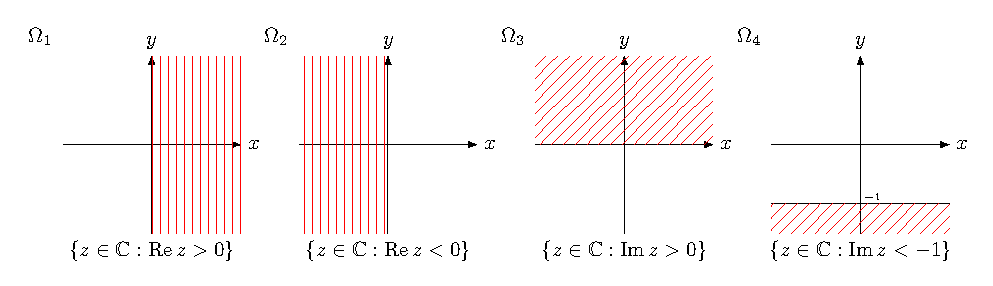
\includegraphics[width=\textwidth]{image_graph1.pdf}

    
\includegraphics{img_graph2.pdf}

    
\includegraphics{img_graph3.pdf}
% \end{align*}
$\{z \in \mathbb{C}: \text{Re } z > 0\} \quad \{z \in \mathbb{C}: \text{Re } z < 0\} \quad \{z \in \mathbb{C}: \text{Im } z > 0\} \quad \{z \in \mathbb{C}: \text{Im } z < -1\}$

But it is not analytic in $\Omega_6$, since $\partial \in \{z \in \mathbb{C}: |z| < 1\}$ and $f$ is not defined at $z = 0$.

$\{z \in \mathbb{C}: |z| > 1\} \quad \{z \in \mathbb{C}: |z| < 1\}$
\end{example}

Note: $f$ is analytic on a domain $\Omega \iff u$ and $v$ are differentiable on $\Omega$ and CR equations hold.

Exercise (Ex 9.3) The function $f(z) = e^x \cos y + ie^x \sin y = e^z$ is entire.

In the next example: a function for which CR equations hold on the whole plane, but $u$ and $v$ are \emphw{not} differentiable on the whole plane, thus the function is \emphic{not}{} entire.

\begin{example}\label{example:9.4}
\[ 
f(z) = \begin{cases}
e^{-1/z^4} & z \neq 0 \\
0 & z = 0
\end{cases}
\text{ defined everywhere in } \mathbb{C} 
\]

\checkthis CR equations hold for every $z \in \mathbb{C}$.
\end{example}
Claim:
\begin{claim} $f(z)$ is not continuous at $z = 0$ ($\implies$ not differentiable).

    \begin{proof}
 Compute $\lim_{z \to 0} f(z)$ on the path $y = x$:
\[ \lim_{\substack{x \to 0 \\ y = x}} e^{-\frac{1}{(x+iy)^4}} = \lim_{x \to 0} e^{-\frac{1}{(1+i)^4 x^4}} = \lim_{x \to 0} e^{\frac{1}{4x^4}} = +\infty \]
$(1 + i)^4 = (\sqrt{2})^4 (\cos(\frac{\pi}{4}) + i\sin(\frac{\pi}{4})) = -4$ De Moivre.
    \end{proof}
\end{claim}
Next proposition is analogous to propositions about the limits, continuity, and differentiability.

\subsection{Properties of analytic functions}

\begin{proposition}\label{proposition:7.1} If $f, g$ are analytic functions on a domain $\Omega$, then also $f + g$ and $f \cdot g$ are analytic on $\Omega$. If $g(z) \neq 0$ on $\Omega$, then $\frac{f}{g}$ is analytic on $\Omega$. The composition $(g \circ f)$ of two analytic functions on $\Omega$ is an analytic function on $\Omega$.

\begin{proof} \emphi{EXERCISE} \end{proof}
\end{proposition}
\begin{example}\label{example:9.5}
    Prove: if $f(z)$ is analytic and real on a domain $\Omega$, then $f$ is a constant function.

\begin{proof} $f$ is analytic and real on $\Omega \implies f(x,y) = u(x,y) + i \cdot 0$, namely $v(x,y) = 0$; CR equations hold for every $z \in \Omega$.
$f$ from analyticity on $\Omega$: $\frac{\partial u}{\partial x} = \frac{\partial v}{\partial y} = 0$ and 
$\frac{\partial u}{\partial y} = -\frac{\partial v}{\partial x} = 0 \implies u(x,y) = c \in \mathbb{R} \implies f(x,y) = c$, namely $f$ is a constant function.
\end{proof}
\end{example}
\begin{proposition} \label{proposition:7.2}
    If $f$ is analytic on a domain $\Omega$ and $f'(z) = 0$ for all $z \in \Omega$, then $f$ is constant on $\Omega$.

\begin{remark}
     Prop 7.2 is false if $\Omega$ is not connected - $f$ can take different constants (constant values) on each connected component of $\Omega$.
\end{remark}
\begin{proof}
    The version of this proposition for real functions is proved using the Mean Value Theorem, 
    that asserts that under appropriate continuity assumption for $f: (a,b) \to \mathbb{R}$ there exists $c \in (a,b)$ s.t. $f(b) - f(a) = f'(c)(b-a)$. 
    So, if $f'(x) = 0$ for all $x \in (a,b)$, then $f(b) = f(a)$. The problem in the complex case is that there is no analogous idea of "between $a$ and $b$" in $\mathbb{C}$, 
    since there are many routes from $a$ to $b$.

    
\includegraphics{img_graph4.pdf}

However, we can use the Mean Value Theorem for Re $f$ and Im $f$ as follows:

Since $f'(z) = 0$ for all $z \in \Omega$ by CR equations $0 = f'(z) = \frac{\partial u}{\partial x} + i\frac{\partial v}{\partial x}$ for all $z \in \Omega \implies \frac{\partial u}{\partial x} = \frac{\partial u}{\partial y} = \frac{\partial v}{\partial x} = \frac{\partial v}{\partial y} = 0$ for all $z \in \Omega$.
\end{proof}

\begin{claim} $u$ is a constant function.
    \begin{proof}
        We have $u: \Omega \to \mathbb{R}, \frac{\partial u}{\partial x} = \frac{\partial u}{\partial y} = 0$ for all $(x,y) \in \Omega$. Pick $(x_0, y_0), (x_1, y_1) \in \Omega$. $\Omega$ is connected, 
        thus by Def~\ref{definition:4.2} any 2 points in $\Omega$ can be connected by a path that is entirely in $\Omega$. 
        We join $(x_0, y_0)$ and $(x_1, y_1)$ by a path comprised of pieces parallel to $x$-axis or 
        $y$-axis [One needs to show that such path exists!] 
        Since $\frac{\partial u}{\partial x} = 0$ by the Mean Value Theorem, $u$ is constant on the horizontal pieces. In the same way,
        since $\frac{\partial u}{\partial y} = 0$, $u$ is constant on vertical pieces. Thus, $u$ is constant on $\Omega$.
        By a similar argument we obtain that $v$ is constant on $\Omega$, therefore $f = u + iv$ is constant on $\Omega$.
    \end{proof}
\end{claim}
\end{proposition}


\includegraphics{img_graph5.pdf}

Now we are going to study analyticity of multi-valued functions - here we will see the big difference between the complex and real functions.

\section{Analyticity of multi-valued functions}

\subsection{Branch points and branches}
We have seen that analytic function is always continuous, thus multi-valued functions are not analytic as is. The question is: can we choose a branch of such function that is single-valued and analytic?

\begin{definition}\label{definition:8.1} We say that on a domain $\Omega$ there is a single-valued 
    branch of multi-valued function if for every point of $\Omega$ we can choose one of the values of a function such that the resulting single-valued function is continuous in $\Omega$.
\end{definition}

In other words: to choose single-valued branch means to choose the domain of definition of a function such that when a point $z$ 
moves along some closed continuous curve that is contained in the domain of definition and goes back to the starting point we get the same value of the function.

Let us demonstrate how we do that on the following example.

\begin{example}\label{example:10.1} 
    Consider double-valued function $f(z) = \sqrt{z - z_0}$. $f(z)$ is defined for all $z \in \mathbb{C}$. Write: $z - z_0 = r(\cos \theta + i\sin \theta), r = |z - z_0|, \theta = \arg(z - z_0)$.

At every $z \neq z_0$, $f(z)$ attains 2 values ($\implies$ double-valued!).
\begin{align*}
    w_0 &= \sqrt{r}\left(\cos \frac{\theta}{2} + i\sin \frac{\theta}{2}\right) \\
    w_1 &= \sqrt{r}\left(\cos\left(\frac{\theta}{2} + \pi\right) + i\sin\left(\frac{\theta}{2} + \pi\right)\right) = -\sqrt{r}\left(\cos \frac{\theta}{2} + i\sin \frac{\theta}{2}\right) = -w_0
\end{align*}

Let us follow the value $w_0$ when $z$ is on the closed continuous curve $L$ that encircles $z_0$ counterclockwise (anti-clockwise; the positive direction).

If $z$ moves to $z_1$, the argument of $z_1 - z_0$ will be
$\arg(z_1 - z_0) = \theta + \theta_1$.


\includegraphics{img_graph6.pdf}

If it continues to move along $L$, $z$ will eventually return to the starting point: the modulus $r = |z - z_0|$ will be the same, 
but the argument will increase by $2\pi$ (since we completed the circle), and $w_0$ will attain the new value $w_1$.
\begin{align*} 
    w_{new} & = \sqrt{r}\left(\cos\left(\frac{\theta + 2\pi}{2}\right) + i\sin\left(\frac{\theta + 2\pi}{2}\right)\right) \\ 
            & = \sqrt{r}\left(\cos\left(\frac{\theta}{2} + \pi\right) + i\sin\left(\frac{\theta}{2} + \pi\right)\right) = w_1 = -w_0 
\end{align*}

Let us check what happens to $w_0$ is we move along a closed continuous curve that does not encircle the point $z_0$.
\end{example}


\includegraphics{img_graph7.pdf}

From the picture above that the value of the modulus and of the argument after completing the full circle will return to its starting value - the same, with no change. 
This is independent of the curve $L_1$ (the only important thing that the curve does not encircle the point $z_0$).
\begin{corollary}\label{corollary:8.1} 
    On a domain $\Omega$ that contains curves that encircle $z_0$, it is impossible to choose a continuous branch of the function $\sqrt{z - z_0}$.
\end{corollary}

% \section*{Lecture Notes,Lectures 11 + 12}
\lecture{11+12}{Continuation and Harmonic functions}

We have studied the double-valued function \( f(z) = \sqrt{z - z_0} \).

Reference, corollary \ref{corollary:8.1}.

For example: On \( \frac{1}{2} < |z - z_0| < 2 \), it is impossible to choose a single-valued branch of \( \sqrt{z - z_0} \).

On \( |z - z_0| > 1 \), it is impossible to choose a single-valued branch of \( \sqrt{z - z_0} \).

We have also seen that if the curve does not encircle \( z_0 \), then the value of \( \sqrt{z - z_0} \) stays the same. 
So, we have another corollary.

\begin{corollary}\label{corollary:8.2}
    It is possible to choose a single-valued branch of the function \( \sqrt{z - z_0} \) on a domain \( \Omega \) 
    if none of the closed continuous curves in \( \Omega \) encircle \( z_0 \).
\end{corollary}

Intuitively, if we would be able to "cut" the plane (in some way) up to \( z_0 \), including \( z_0 \), then there will be no closed curve that encircles \( z_0 \).
Indeed, the biggest domain on which none of the closed continuous curves encircle \( z_0 \) is the cutted plane, where we cut as follows.

\subsection*{The "largest" such domain}
\begin{itemize}
    \item Cut-plane: \( \mathbb{C} \) without the line \( \{ z = x + iy \mid x \leq x_0 \} \) 
    (including \( z_0 \)).
    
    
\includegraphics{img_graph8.pdf}

    \item Cut-plane: two single-valued branches:
    \[
        w_0 = \sqrt{r} (\cos \frac{\theta}{2} + i \sin \frac{\theta}{2}), \quad 
        w_1 = -\sqrt{r} (\cos \frac{\theta}{2} + i \sin \frac{\theta}{2})
    \]

    
\includegraphics{img_graph9.pdf}
\end{itemize}

\emphOnly{Note}: We can cut along any ray starting at \( z_0 \).

The cut will prevent any closed curve from encircling \( z_0 \). In the case of the line in the picture above (ray creates an angle \( \theta \) with the positive counterclockwise direction with the \( x \)-axis), we have:

For a ray with \( \theta = \frac{\pi}{4} \), two continuous branches of \( \sqrt{z - z_0} \):

\[
    w = \pm \sqrt{r} (\cos \frac{\theta}{2} + i \sin \frac{\theta}{2}), \quad \frac{\pi}{4} < \theta \leq \frac{5\pi}{4}
\]

\begin{definition}\label{definition:8.2} The point \( z_0 \) is called a \textit{branch point} for a complex multi-valued function if the value of \( f(z) \) does not return to its initial value as a closed curve around the point is traced (starting from some arbitrary point on the curve) in such a way that \( f \) varies continuously as the path is traced.
\end{definition}
\textbf{Important:} What matters here is the \textbf{local} behavior of the function \( f \) near \( z_0 \). What may happen on paths that are some distance away from \( z_0 \) is not relevant. To be more precise:

\noindent \textbf{The behavior must occur for all the curves that enclose the point and are sufficiently close to it.}

In example \ref{example:10.1} \( z = z_0 \) is the \textbf{Branch Point}.

Let us consider a more general case.


\begin{example} Consider \( w = \sqrt[n]{z - z_0} \). Take \( z - z_0 = r (\cos \theta + i \sin \theta) \). Then:

\[
w_k = \sqrt[n]{r} \left( \cos \frac{\theta + 2\pi k}{n} + i \sin \frac{\theta + 2\pi k}{n} \right), \quad k = 0,1,2, \dots, n-1.
\]

Fix \( 0 \leq k_0 \leq n-1 \).

As before, we let \( z \) be on the closed continuous curve \( L \) that encloses \( z_0 \). 


\includegraphics{img_graph10.pdf}

When \( z \) will complete the full circle (anticlockwise), the modulus \( r \) will return to the same value. The argument, however, will increase by \( 2\pi \), and \( w \) will attain a new value.
% \end{example}
\emphic{After full circle around $z_0 $:}{}
\[
w = \sqrt[n]{r} \left( \cos \frac{(\theta + 2\pi) + 2\pi k_0}{n} + i \sin \frac{(\theta + 2\pi) + 2\pi k_0}{n} \right).
\]

\[
= \sqrt[n]{r} \left( \cos \frac{\theta + 2\pi k_0}{n} + i \sin \frac{\theta + 2\pi k_0}{n} \right) 
\cdot \left( \cos \frac{2\pi}{n} + i \sin \frac{2\pi}{n} \right).
\]

\[
= w_{k_0} \left( \cos \frac{2\pi}{n} + i \sin \frac{2\pi}{n} \right) = w_{k_0 + 1}.
\]
\end{example}

Namely, the new value of \( w \) is equal to the previous one times \( \left( \cos \frac{2\pi}{n} + i \sin \frac{2\pi}{n} \right) \).

\checkthis{}

\[
\left( \cos \frac{2\pi}{n} + i \sin \frac{2\pi}{n} \right)^n = 1.
\]

This is independent of the curve that encloses \( z_0 \). If \( z \) runs on a curve that does not encircle \( z_0 \), then, as before, the value \( w_{k_0} \) will not change once \( z \) returns to the starting point.

\textbf{Conclusion:} If \( z \) is on the curve that encloses \( z_0 \) once (anticlockwise), then the value \( \sqrt[n]{z - z_0} = w_{k_0} \) will change to the new value \( w_{k_0 + 1} \). If \( z \) is on the curve that does not enclose \( z_0 \), 
then the value of the function stays the same.
$\implies z = z_0$ is the branch point of the function $f(z) = \sqrt[n]{z - z_0}$.

\begin{example}\label{example:10.3} Find the branch points of the function $f(z) = \sqrt{1 + z^2}$.
    \begin{soln}
        $\sqrt{1 + z^2} = \sqrt{z - i} \cdot \sqrt{z + i}$, therefore $z = \pm i$ are the branch points of $\sqrt{z - i}$, $\sqrt{z + i} \implies$ branch points of $\sqrt{1 + z^2}$.
Let us see on the picture what happens and where to cut so we will be able to obtain a continuous single-valued branch of $f(z)$.

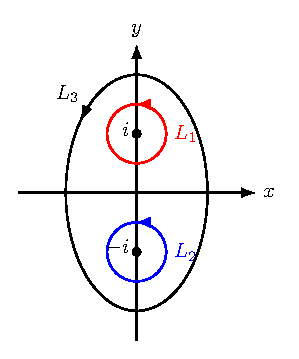
\includegraphics{img_graph11.pdf}

If $z$ is on $L_1$ (around $z = i$): when $z$ returns to the initial point $\sqrt{z + i}$ returns to the same value since $L_1$ does not enclose $z = -i$ while $\sqrt{z - i}$ attains new value - changes the sign of the previous one. Therefore, $f(z)$ also changes the sign. In the same way: if $z$ is on $L_2$, then upon return to the initial point $\sqrt{z + i}$ will change the value - change the sign, $\sqrt{z - i}$ will return to the same value, and the function will change the sign. If $z$ is on $L_3$ that encloses both $z_0 = i$ and $z_0 = -i$, then $\sqrt{z - i}$ and $\sqrt{z + i}$ will change the sign, but their product - the original function - will not!
    \end{soln}
\end{example}

$\implies$ We can choose a continuous branch on a domain $\Omega$ if none of the closed curves in $\Omega$ enclose $i$ and not $-i$ (or $-i$ and not $i$), but it can enclose both. Namely, if we cut the plane along the interval connecting $i$ and $-i$, we will get a domain in which it is possible to choose a continuous branch.

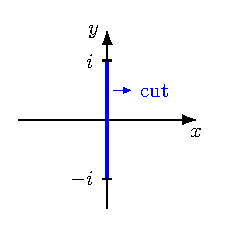
\includegraphics{img_graph12.pdf}

\begin{definition}\label{definition:8.3} Single-valued branch is called an analytic function on a domain $\Omega$ if it is differentiable at every $z \in \Omega$.
\end{definition}

\begin{example}\label{example:10.4} Prove that $w = \sqrt[n]{z}$ is analytic on the domain $\Omega = \{z \in \mathbb{C}: 0 < \arg z < \frac{2\pi}{n}\}$.

\begin{proof}    We have already seen that on the cut-plane with the cut
along any ray starting at $z_0 = 0$ (including $z_0 = 0$) every branch of this function is single-valued and continuous. Let us prove that it is differentiable and find the derivative.

\begin{align*}  & \frac{f(z) - f(z_0)}{z - z_0} = \frac{(f(z))^n - (f(z_0))^n}{z - z_0} \\ 
                & = \frac{1}{(\sqrt[n]{z})^n - (\sqrt[n]{z_0})^n} \cdot \frac{(f(z))^{n-1} + (f(z))^{n-2}f(z_0) + \dots + (f(z_0))^{n-1}}{z - z_0} \\
                & = \frac{1}{(\sqrt[n]{z})^{n-1} + (\sqrt[n]{z})^{n-2}\sqrt[n]{z_0} + \dots + (\sqrt[n]{z_0})^{n-1}} \end{align*}

Now we pass to the limit as $z$ tends to $z_0$ and obtain
\[ \implies \lim_{z \to z_0} \frac{f(z) - f(z_0)}{z - z_0} = \frac{1}{n(\sqrt[n]{z_0})^{n-1}} \]
$\implies f$ is differentiable and \[ (\sqrt[n]{z})' = \frac{1}{n(\sqrt[n]{z})^{n-1}}.\]
\end{proof}
\end{example}

In many problems in hydrodynamics, the elasticity theory and other fields there is often a need to recreate an analytic function from its real part. Now we will find the set of functions for which it is possible. Our subject is:

\section{Harmonic functions.}

\subsection{Definitions and basic results}

\begin{definition}\label{definition:9.1} The real function $u(x,y)$ is called harmonic on a domain $\Omega$ if it is continuous on $\Omega$ with continuous partial derivatives of the first and second order 
    \[\{\frac{\partial u}{\partial x}, \frac{\partial u}{\partial y}, \frac{\partial^2 u}{\partial x^2}, \frac{\partial^2 u}{\partial y^2}, \frac{\partial^2 u}{\partial x \partial y}, \frac{\partial^2 u}{\partial y \partial x}\},\] and the following equation, called the Laplace equation, holds:
\[ \frac{\partial^2 u}{\partial x^2} + \frac{\partial^2 u}{\partial y^2} = 0 \]
\end{definition}

\begin{example}\label{example:11.1} The function $u(x,y) = x^2 - y^2$ is harmonic for every $(x,y) \in \mathbb{R}^2$.
\begin{soln}
         $u(x,y)$ is defined everywhere, and we have:
    $\frac{\partial u}{\partial x} = 2x \quad \frac{\partial u}{\partial y} = -2y \quad \frac{\partial^2 u}{\partial x^2} = 2 \quad \frac{\partial^2 u}{\partial y^2} = -2 \quad \frac{\partial^2 u}{\partial x \partial y} = \frac{\partial^2 u}{\partial y \partial x} = 0$
    
    All partial derivatives are continuous everywhere, and $\frac{\partial^2 u}{\partial x^2} + \frac{\partial^2 u}{\partial y^2} = 2 + (-2) = 0$.
\end{soln}
\end{example}

\begin{example}\label{example:11.2} The function $u(x,y) = e^x y$ is \textbf{not} harmonic function on $\mathbb{R}^2$.
\begin{proof} $u(x,y)$ is defined everywhere on $\mathbb{R}^2$.

\begin{align*}
    & \frac{\partial u}{\partial x} = ye^{xy} \qquad & \frac{\partial u}{\partial y} &= xe^{xy} \\ 
    & \frac{\partial^2 u}{\partial x^2} = y^2e^{xy} \qquad & \frac{\partial^2 u}{\partial y^2} &= x^2e^{xy} \\
    & \frac{\partial^2 u}{\partial x \partial y} = e^{xy} + yxe^{xy} \qquad & \frac{\partial^2 u}{\partial y \partial x} &= e^{xy} + xye^{xy} 
\end{align*}

All partial derivatives are defined and continuous for all $(x,y) \in \mathbb{R}^2$. However $\frac{\partial^2 u}{\partial x^2} + \frac{\partial^2 u}{\partial y^2} = y^2e^{xy} + x^2e^{xy} = e^{xy}(x^2 + y^2) \neq 0$ except for $(0,0) \implies u(x,y)$ is \textbf{not} harmonic function on $\mathbb{R}^2$.
\end{proof}
\end{example}

\begin{proposition}\label{proposition:9.1} If the function $f(z) = u(x,y) + iv(x,y)$ is analytic on a domain $\Omega$, then $u(x,y)$ and $v(x,y)$ are harmonic on $\Omega$.
\end{proposition}

    \begin{proof}
By CR equations $\frac{\partial u}{\partial x} = \frac{\partial v}{\partial y}$ and $\frac{\partial u}{\partial y} = -\frac{\partial v}{\partial x}$ (since $f$ is analytic). Let us differentiate the first equation with respect to $x$ and the second with respect to $y$:
\[ \frac{\partial^2 u}{\partial x^2} = \frac{\partial^2 v}{\partial y \partial x}, \quad \frac{\partial^2 u}{\partial y^2} = -\frac{\partial^2 v}{\partial x \partial y} \]
Since $f$ is analytic, $u$ and $v$ are continuously differentiable, thus from theory of real functions, we know that $\frac{\partial^2 v}{\partial y \partial x} = \frac{\partial^2 v}{\partial x \partial y}$. Therefore, if we add the equations (*), we obtain:
\[ \frac{\partial^2 u}{\partial x^2} + \frac{\partial^2 u}{\partial y^2} = \frac{\partial^2 v}{\partial y \partial x} - \frac{\partial^2 v}{\partial x \partial y} = \frac{\partial^2 v}{\partial x \partial y} - \frac{\partial^2 v}{\partial x \partial y} = 0 \]
$\implies u$ is harmonic function on $\Omega$.

If we differentiate now $\frac{\partial u}{\partial x} = \frac{\partial v}{\partial y}$ with respect to $y$ and $\frac{\partial u}{\partial y} = -\frac{\partial v}{\partial x}$ with respect to $x$, and use $\frac{\partial^2 u}{\partial x \partial y} = \frac{\partial^2 u}{\partial y \partial x}$ we will obtain that $v$ is also harmonic function on $\Omega$.
    \end{proof}

This proposition implies that in order to construct an analytic function we cannot choose the real and imaginary parts in an arbitrary way. The functions that we choose must be harmonic and, moreover, the CR equations must hold.

\begin{definition}\label{definition:9.2} If $u(x,y)$ and $v(x,y)$ are harmonic functions on a domain $\Omega$ such that CR equations hold ($\frac{\partial u}{\partial x} = \frac{\partial v}{\partial y}, \frac{\partial u}{\partial y} = -\frac{\partial v}{\partial x}$), then the function $v(x,y)$ is called the \emphw{harmonic conjugate} of the function $u(x,y)$ on a domain $\Omega$.
\end{definition}
\begin{proposition}\label{proposition:9.2} The function $f(z) = u(x,y) + iv(x,y)$ is analytic in a domain $\Omega \iff v(x,y)$ is the harmonic conjugate of $u(x,y)$.
\end{proposition}

\begin{proof} [$\implies$] Assume $f$ is analytic in a domain $\Omega$. By Prop~\ref{proposition:9.1}
$u(x,y)$ and $v(x,y)$ are harmonic functions on $\Omega$. Since $f$ is analytic, CR equations hold, thus by Def~\ref{definition:9.2} $v(x,y)$ is the harmonic conjugate of $u(x,y)$.

[$\impliedby$] If $u(x,y)$ and $v(x,y)$ are harmonic functions on a domain $\Omega$, then $u$ and $v$ are differentiable at all $z \in \Omega$. Since $v(x,y)$ is the harmonic conjugate of $u(x,y)$, 
by Def~\ref{definition:9.2} - CR equations hold, 
thus Thm 6.1 \ref{theorem:6.1} asserts that $f$ is analytic in a domain $\Omega$.
\end{proof}

Thus, to conclude that we can reconstruct an analytic function from its real part we need to know whether it is always possible to find a harmonic conjugate to a given harmonic function. The answer is yes - it is given by the following proposition which we state without the proof.

\begin{proposition}\label{proposition:9.3} For any harmonic function $u(x,y)$ in a domain $\Omega$ there exists a function $v(x,y)$ in $\Omega$ which is the harmonic conjugate of $u(x,y)$.

The proof is by construction: one explicitly constructs the function $v(x,y)$. Since the proof involves somewhat complicated real analysis, we omit it.
\end{proposition}

\begin{example}\label{example:11.3} Find an analytic function $f(z) = u(x,y) + iv(x,y)$ such that $u(x,y) = \text{Re } f(z) = \arctan \frac{y}{x}$.

\begin{soln} Let us compute the partial derivatives and then use CR equations: Recall: $(\arctan x)' = \frac{1}{1 + x^2}$
\[ \frac{\partial u}{\partial x} = \frac{-y}{x^2 + y^2} \qquad \frac{\partial u}{\partial y} = \frac{x}{x^2 + y^2} \implies \frac{\partial v}{\partial y} = \frac{-y}{x^2 + y^2}, \frac{\partial v}{\partial x} = \frac{-x}{x^2 + y^2} \]
CR equations

To obtain $v(x,y)$ we integrate $\frac{\partial v}{\partial x}$ with respect to $x$ (or $\frac{\partial v}{\partial y}$ with respect to $y$).
\[ v(x,y) = \int \frac{\partial v}{\partial x} dx = \int \frac{-x}{x^2 + y^2} dx = -\frac{1}{2} \ln(x^2 + y^2) + c(y) \]
Since the integral is with respect to $x$, the constant may depend on $y$ (only!) To find $c(y)$ we differentiate $v(x,y)$ in (*) with respect to $y$ and compare it to $\frac{\partial v}{\partial y}$ obtained from CR equations:
\[ \frac{\partial v}{\partial y} = \frac{-y}{x^2 + y^2} + c'(y) = \frac{-y}{x^2 + y^2} \implies c'(y) = 0 \implies c = \text{constant} \in \mathbb{R} \]
$\implies v(x,y) = -\frac{1}{2}\ln(x^2 + y^2) + c$ and $f(z) = \arctan \frac{y}{x} - \frac{i}{2}[\ln(x^2 + y^2) + 2c]$.

\end{soln}
\end{example}
%\usepackage{xr}

% \externaldocument{note01}
% \externaldocument{note02}
% \externaldocument{note03}
% \externaldocument{note04}
% \externaldocument{note05}
% \externaldocument{note06}
% \externaldocument{note07}
% \externaldocument{note08}
% \externaldocument{note09}
% \externaldocument{note10}
% \externaldocument{note11}

\graphicspath{{./input/graphs/note05/}}


% \zexternaldocument{note01}
% \zexternaldocument{note02}
% \zexternaldocument{note03}
% \zexternaldocument{note04}
% \zexternaldocument{note05}
% \zexternaldocument{note06}
% \zexternaldocument{note07}
% \zexternaldocument{note08}
% \zexternaldocument{note09}
% \zexternaldocument{note10}
% \zexternaldocument{note11}
% \externaldocument{note12}



\week{5}
% \section*{Week 5. Lecture 13.}
\lecture{13}{Sequences in $\mathbb{C}$}
We introduce complex sequences and series, discuss their convergence and use them to construct complex power series. Then, we make several concrete connections with complex differentiable functions.

\section{Complex sequences.}

\subsection{Sequence limits}

\begin{definition}\label{definition:10.1} A sequence $\{z_n\}_{n=0}^{\infty}, z_n \in \mathbb{C}$, has limit $z$ (as $n \to \infty$) if for every $\epsilon > 0$ there exists $N = N(\epsilon) \in \mathbb{N}$ such that for all $n > N$, $|z_n - z| < \epsilon$. Notation: $\lim_{n \to \infty} z_n = z$.
\end{definition}
If the limit does not exist (or $\infty$), we say that the sequence diverges.

In other words, a sequence of complex numbers $\{z_n\}$ converges to the complex number $z$ iff at every neighborhood of $z$ there are almost all but finite number of points from the sequence: $\lim_{n \to \infty} z_n = z \iff \forall \epsilon > 0 \quad \exists N(\epsilon) \in \mathbb{N} \text{ s.t. for every } n > N(\epsilon) \quad |z_n - z| < \epsilon$.

\begin{claim}
If $\lim_{n \to \infty} z_n$ exists, then it is unique.
\begin{proof}
Assume $\lim_{n \to \infty} z_n = \tilde{z_1}$ and $\lim_{n \to \infty} z_n = \tilde{z_2}$. Then, for any $\epsilon > 0$ there exists $N_1 \in \mathbb{N}$ s.t. 
for every $n > N_1$, $|z_n - \tilde{z_1}| < \epsilon/2$. Also there exists $N_2 \in \mathbb{N}$ s.t. for every $n > N_2$, $|z_n - \tilde{z_2}| < \epsilon/2$. 
Choose $N = \max\{N_1, N_2\}$, then for every $n > N$, $|z_n - \tilde{z_1}| < \epsilon/2$ and $|z_n - \tilde{z_2}| < \epsilon/2$.

Thus $|\tilde{z_1} - \tilde{z_2}| = |\tilde{z_1} - z_n + z_n - \tilde{z_2}| \leq |\tilde{z_1} - z_n| + |z_n - \tilde{z_2}| < \epsilon/2 + \epsilon/2 = \epsilon$. Since this is true for any $\epsilon > 0$ we conclude that $\tilde{z_1} = \tilde{z_2}$.
\end{proof}
\end{claim}
Also, it is possible to show that the complex sequence $\{z_n\}$ converges to $z \iff$ the real sequence $\{|z_n - z|\}_{n=0}^{\infty}$ converges to 0 (\verifythis)

\begin{example}\label{example:12.1} Let $z_n = (\frac{i}{2})^n, n \in \mathbb{N}$. Then: $z_0 = 1, z_1 = \frac{i}{2}, z_2 = \frac{i^2}{4} = -\frac{1}{4}, z_3 = \frac{i^3}{8} = -\frac{i}{8}, z_4 = \frac{i^4}{16} = \frac{1}{16}, \dots$
\end{example}
This sequence converges to 0: $\lim_{n \to \infty} z_n = 0$. Can be demonstrated by proving that $|z_n|$ decreases to 0 as $n$ tends to infinity. (\checkthis{} By graphing the points $z_n$ check that the sequence
$\{z_n\}$ "spirals" in toward the origin $(0)$ in the $z$-plane.

\begin{example}\label{example:12.2} Let $z_n = (2i)^n: z_0 = 1, z_1 = 2i, z_2 = -4, z_3 = -8i, \dots$. This sequence diverges: one can show that $\{|z_n|\}_{n=0}^{\infty}$ is unbounded increasing sequence \{namely, $|z_n|$ gets arbitrarily large\}.
\end{example}

\begin{example}\label{example:12.3} Let $z_n = (i)^n: z_0 = 1, z_1 = i, z_2 = -1, z_3 = -i, z_4 = 1, z_5 = i, \dots$. This is a bounded sequence ($|z_n| \leq 1$ for any $n$), but $\lim_{n \to \infty} z_n$ does not exist: there is no $z$ such that almost all but finitely many points of the sequence are in a small neighborhood of some $z$: 
    
    
\includegraphics{img_graph1.pdf}
    
    $z_n$ jumps at every step.
\end{example}

Important real sequence (limit): let $a_n = (1 + \frac{a}{n})^n$ for some $a$. Then $\lim_{n \to \infty} a_n = (1 + \frac{a}{n})^n = e^a$.

\begin{example}\label{example:12.4} $\lim_{n \to \infty} (1 + \frac{i}{n})^n = e^i, \quad \lim_{n \to \infty} (1 - \frac{i}{n})^n = \lim_{n \to \infty} (1 + \frac{-i}{n})^n = e^{-i} = \frac{1}{e^i}$.
\end{example}

\begin{proposition} \zlabel{proposition:10.1} 
    If the sequences $\{z_n\}, \{w_n\}$ of complex numbers converge, then so the sequences $\{z_n \pm w_n\}, \{z_n \cdot w_n\}$, 
    and if $w_n \neq 0$ also $\{\frac{z_n}{w_n}\}$, and 
    \[\lim_{n \to \infty} (z_n \pm w_n) = \lim_{n \to \infty} z_n \pm \lim_{n \to \infty} w_n; \quad \lim_{n \to \infty} z_n w_n = \lim_{n \to \infty} z_n \lim_{n \to \infty} w_n.\]

If $\lim_{n \to \infty} w_n \neq 0$, then: $\lim_{n \to \infty} \frac{z_n}{w_n} = \frac{\lim_{n \to \infty} z_n}{\lim_{n \to \infty} w_n}$.
\end{proposition}

\section{Complex (scalar) series.}

\subsection{Series convergence}

\begin{definition}\label{definition:11.1} 
    The complex (scalar) series $\sum_{n=1}^{\infty} z_n$ converges to the value $s \in \mathbb{C}$ if the sequence of partial sums $\{S_N\}_{N=0}^{\infty}, S_N = z_0 + z_1 + \dots + z_N$ converges to $s$. 
    The value $s$ is called the sum of the series. If the limit does not exist (or $\infty$) ($\lim_{N \to \infty} S_N$) then the series diverges. If the series converges to some value $s$, then $s$ is unique.
\end{definition}

\begin{remark}
Furthermore: if $r_N = S - S_N = \sum_{n=N+1}^{\infty} z_n$, then it is possible to show that $\sum_{n=0}^{\infty} z_n = S \iff \lim_{N \to \infty} r_N = 0$. 
Namely, the \emphi{tail} of the series converges to 0.
\end{remark}
From Def (\ref{definition:11.1}) we immediately conclude:
\begin{proposition}\label{proposition:11.1} If $\sum_{n=0}^{\infty} z_n$ converges, then $\lim_{n \to \infty} z_n = 0$.
\begin{proof}
    By Def (\ref{definition:11.1}): If $\sum_{n=0}^{\infty} z_n = S$, then $\lim_{N \to \infty} S_N = \lim_{N \to \infty} \sum_{n=0}^{N} z_n = S$. On the other hand: $S_N - S_{N-1} = (z_0 + z_1 + \dots + z_N) - (z_0 + z_1 + \dots + z_{N-1}) = z_N$
    $\implies \lim_{N \to \infty} z_N = \lim_{N \to \infty} (S_N - S_{N-1}) = \lim_{N \to \infty} S_N - \lim_{N \to \infty} S_{N-1} = S - S = 0$ by Prop 10.1(\zref{proposition:10.1}). $s$ is unique.
\end{proof}
\end{proposition}
The contrapositive statement is often called the Test for Divergence.

\begin{proposition}[Test for Divergence]\label{proposition:11.2} (Test for Divergence) Let $\{z_n\}_{n=0}^{\infty} \in \mathbb{C}$. If $\lim_{n \to \infty} z_n \neq 0$ (or does not exist), then the series $\sum_{n=0}^{\infty} z_n$ diverges.
\end{proposition}

\begin{remark}
The converse of Prop 11.2(\ref{proposition:11.2}) is false: $\lim_{n \to \infty} \frac{1}{n} = 0$, but the series $\sum_{n=1}^{\infty} \frac{1}{n}$ diverges!
\end{remark}
As expected there is an immediate relation between convergence or divergence of complex sequences and series to that of real ones.

\begin{proposition}\label{proposition:11.3} Let $\{z_n\}_{n=0}^{\infty}, z_n$ be the complex sequence and the complex series. Suppose that $z = x + iy$ and $S = u + iv$. Then:
\begin{enumerate}
    \item $\lim_{n \to \infty} z_n = z \iff \lim_{n \to \infty} x_n = x$ and $\lim_{n \to \infty} y_n = y$ (for $z_n = x_n + iy_n$)
    \item $\sum_{n=0}^{\infty} z_n = S \iff \sum_{n=0}^{\infty} x_n = u$ and $\sum_{n=0}^{\infty} y_n = v$
\end{enumerate}
\begin{proof}
    \begin{enumerate}
        \item follows directly from Def 10.1(\ref{definition:10.1}) and the application of triangle inequality: $|x_n - x|, |y_n - y| \leq |z_n - z| \leq |x_n - x| + |y_n - y|$
        \item is proved by decomposing the complex sum into real and imaginary parts $\sum_{n=0}^{\infty} z_n = \sum_{n=0}^{\infty} x_n + i\sum_{n=0}^{\infty} y_n$ and a careful use of 1) [FINISH!]
    \end{enumerate}
\end{proof}
\end{proposition}

Hint: If $\sum_{n=0}^{\infty} x_n = u, \sum_{n=0}^{\infty} y_n = v \implies$ obvious. Assume $\sum_{n=0}^{\infty} z_n = S$, define $X_N = \sum_{n=0}^{N} x_n, Y_N = \sum_{n=0}^{N} y_n$, apply 1) to $S_N = \sum_{n=0}^{N} z_n$.

In much of what follows, we can use Prop 11.3 and results in real sequences and series - these are left as an exercise. For example, Prop 10.1 and an analogous proposition for the series:

\begin{proposition} \label{proposition:11.4} Suppose that $\sum_{n=0}^{\infty} z_n = S, \sum_{n=0}^{\infty} w_n = t$ are two convergent series. Let $\alpha \in \mathbb{C}$. Then,
\begin{enumerate}
    \item $\sum_{n=0}^{\infty} (z_n \pm w_n) = S \pm t$ (converges to $S \pm t$)
    
    \item $\sum_{n=0}^{\infty} \alpha z_n = \alpha S$ (converges to $\alpha S$)
\end{enumerate}

\begin{proof} (EXERCISE - exactly as in the real case - partial sums).
\end{proof}
\end{proposition}

\begin{example} \label{example:13.1} (Key example - Geometric series)

Suppose that $|z| < 1$. We claim that the series $\sum_{n=0}^{\infty} z^n$, called the Geometric series, converges.
\begin{claim}\label{claim:11.5}
    $\sum_{n=0}^{\infty} z^n$ converges (if $|z| < 1$) and $\sum_{n=0}^{\infty} z^n = \frac{1}{1-z}$.
\end{claim}
\begin{proof}
    We prove it using Def 11.1: we will show that the sequence of partial sums converges to $\frac{1}{1-z}$.
    Need to show: $\lim_{N \to \infty} S_N = \lim_{N \to \infty} \sum_{n=0}^{N} z^n = \frac{1}{1-z}$.
    
    First, we obtain a closed formula for $S_N$ as follows.
    \begin{align*}
        S_N &= 1 + z + z^2 + \dots + z^N \\
        z \cdot S_N &= z + z^2 + z^3 + \dots + z^{N+1} \\
        &\implies S_N - zS_N = S_N(1-z) = 1 - z^{N+1} \\
        &\implies S_N = \frac{1 - z^{N+1}}{1-z}
    \end{align*}
\end{proof}
Now we use this formula to compute the limit
\[ \left| \frac{1}{1-z} - S_N \right| = \left| \frac{1}{1-z} - \frac{1 - z^{N+1}}{1-z} \right| = \left| \frac{z^{N+1}}{1-z} \right| = \frac{|z|^{N+1}}{|1-z|} \]
Since $|z| < 1 \implies \lim_{N \to \infty} |z|^N = 0$ (from what we know about real sequences). Therefore $\left| \frac{1}{1-z} - S_N \right| \xrightarrow{N \to \infty} 0 \implies \lim_{N \to \infty} S_N = \frac{1}{1-z}$.
\end{example}

% \section*{Lectures 14+15.}
\lecture{14+15}{Absolute convergence?! WTH is that?}

Now we introduce the notion of absolute convergence.

\begin{definition}\label{definition:11.2} The series $\sum_{n=0}^{\infty} z_n$ converges absolutely if the series of the moduli of the terms $\sum_{n=0}^{\infty} |z_n|$ converges.
\end{definition}

\begin{remark}
Note: (The Geometric series) For $|z| < 1$, $\sum_{n=0}^{\infty} |z|^n$ converges. Namely, the geometric series converges absolutely.
\begin{proof}
    Follow exactly the same steps as in Ex 13.1, replace $z$ by $|z|$.
\end{proof}
\end{remark}

The definition of absolute convergence is subtle: Series can converge, but not absolutely: $\sum_{n=1}^{\infty} \frac{(-1)^n}{n}$ converges, but $\sum_{n=1}^{\infty} |\frac{(-1)^n}{n}| = \sum_{n=1}^{\infty} \frac{1}{n}$ diverges.

The absolute convergence *however* always implies convergence:

\begin{proposition}\label{proposition:11.6} If $\sum_{n=0}^{\infty} |z_n|$ converges, then $\sum_{n=0}^{\infty} z_n$ converges.
\begin{proof}
    We have $|z_n| = \sqrt{x_n^2 + y_n^2} \geq |x_n|, |y_n|$, therefore using the Comparison test for positive (real) series we get that $\sum_{n=0}^{\infty} |x_n|$ 
    and $\sum_{n=0}^{\infty} |y_n|$ converge $\implies$ (by analogous statement for real series) $\sum_{n=0}^{\infty} x_n$ and $\sum_{n=0}^{\infty} y_n$ converge. 
    Thus, by Prop 11.3(\ref{proposition:11.3}) 2) $\sum_{n=0}^{\infty} z_n$ converges.
\end{proof}
\end{proposition}

Now we state 3 very useful tests for convergence of complex series.

\begin{proposition} \label{proposition:11.7} Let $\sum_{n=0}^{\infty} a_n, a_n \in \mathbb{C}$ be a complex series.

\begin{enumerate}
    \item \textbf{Ratio-Test:} Consider the limit $\lim_{n \to \infty} \left| \frac{a_{n+1}}{a_n} \right| = \lim_{n \to \infty} \frac{|a_{n+1}|}{|a_n|} = L$
    \begin{itemize}
        \item If the limit exists and $L < 1$, then the series $\sum_{n=0}^{\infty} a_n$ converges absolutely.
        \item If the limit exists and $L > 1$, then the series $\sum_{n=0}^{\infty} a_n$ diverges.
        \item If $L = 1$ or the limit does not exist, then the test is inconclusive \{namely, there are examples of convergent and divergent series\}.
    \end{itemize}
    \item \textbf{Root (Cauchy) Test:} Consider the limit $\lim_{n \to \infty} \sqrt[n]{|a_n|} = L$
    \begin{itemize}
        \item If the limit exists and $L < 1$, then the series $\sum_{n=0}^{\infty} a_n$ converges absolutely.
        \item If the limit exists and $L > 1$, then the series $\sum_{n=0}^{\infty} a_n$ diverges.
        \item If $L = 1$ or does not exist, then the test is inconclusive.
    \end{itemize}
    \item \textbf{Comparison Test:}
    \begin{itemize}
        \item If $0 \leq |a_n| < r_n$ and the positive real series $\sum_{n=0}^{\infty} r_n$ converges, then $\sum_{n=0}^{\infty} a_n$ converges absolutely.
        \item If $|a_n| > r_n \geq 0$ and $\sum_{n=0}^{\infty} r_n$ diverges, then $\sum_{n=0}^{\infty} a_n$ diverges.
    \end{itemize}

\end{enumerate}
\end{proposition}
\begin{proof}
    Ratio Test: If $L > 1$, then the sequence $\{|a_n|\}$ is increasing (for sufficiently large $n$), therefore the series diverges by the Test for Divergence.
    
    Suppose that $L < 1$. Choose a number $r$ such that $L < r < 1$. Since $\lim_{n \to \infty} \left| \frac{a_{n+1}}{a_n} \right| = L$ there exists $N \in \mathbb{N}$ such that for all $n \geq N: \left| \frac{|a_{n+1}|}{|a_n|} - L \right| < \epsilon$. Set $\epsilon = a_N$. Then we have $|a_{N+1}| \leq r|a_N| = |a|r$, $|a_{N+2}| \leq r|a_{N+1}| < |a|r^2$ and, in general $|a_{N+k}| \leq |a|r^k$. Therefore for $n \geq N$ the terms of the series $\sum_{n=0}^{\infty} |a_n|$ are bounded by the terms of a convergent geometric series (since $0 \leq r < 1$), therefore $\sum_{n=0}^{\infty} |a_n|$ converges by the Comparison Test (for real series), namely, $\sum_{n=0}^{\infty} a_n$ converges absolutely.
    
    Root Test and Comparison Test: EXERCISE!
\end{proof}

\begin{example}\label{example:13.2} Check the convergence of the following series:
    \begin{enumerate}
        \item  $\sum_{n=0}^{\infty} (2i)^n$ 
        \item  $\sum_{n=0}^{\infty} \left(\frac{1+i}{2}\right)^n$ 
        \item  $\sum_{n=0}^{\infty} \frac{(4i)^n}{n!}$
    \end{enumerate}
\begin{soln}
    \begin{enumerate}
        \item We use Comparison Test as follows: $a_n = (2i)^n \implies |a_n| = (|2i|)^n = |2|^n = 2^n > (\frac{3}{2})^n$. Since $\sum_{n=0}^{\infty} (\frac{3}{2})^n$ diverges (for example, by the Test for Divergence, since $\lim_{n \to \infty} (\frac{3}{2})^n = \infty \neq 0$) by Comparison Test $\sum_{n=0}^{\infty} (2i)^n$ diverges.
    
        \item Let us apply the Root Test: $a_n = \left(\frac{1+i}{2}\right)^n$
    $\implies \lim_{n \to \infty} \sqrt[n]{|a_n|} = \lim_{n \to \infty} \sqrt[n]{\left|\frac{1+i}{2}\right|^n} = \lim_{n \to \infty} \frac{|1+i|}{2} = \frac{\sqrt{2}}{2} = \frac{1}{\sqrt{2}} < 1$
    $\implies \sum_{n=0}^{\infty} \left(\frac{1+i}{2}\right)^n$ converges absolutely.
    
    \item Let us apply the Ratio Test: $a_n = \frac{(4i)^n}{n!}$
    
    \begin{align*}
         \implies \lim_{n \to \infty} \left| \frac{a_{n+1}}{a_n} \right| = \lim_{n \to \infty} \left| \frac{\frac{(4i)^{n+1}}{(n+1)!}}{\frac{(4i)^n}{n!}} \right| &= \lim_{n \to \infty} \left| \frac{(4i)^{n+1}}{(n+1)!} \cdot \frac{n!}{(4i)^n} \right| \\
         & = \lim_{n \to \infty} \frac{|4i|}{n+1} = \lim_{n \to \infty} \frac{4}{n+1} = 0 < 1 
    \end{align*}
    
    $\implies $ converges absolutely.
    \end{enumerate}
\end{soln}
\end{example}

\section{Complex Power Series}

\subsection{Power series basics}
\begin{definition}\label{definition:12.1} 
    The series $\sum_{n=0}^{\infty} a_n(z-z_0)^n, a_n \in \mathbb{C}, n \in \mathbb{N}$, is called a power series centered at $z = z_0$ (about $z = z_0$).
\end{definition}

A power series is an example of complex series where the sequence $z_n$ from Def 11.1(\ref{definition:11.1}) is of the special form $\{a_n(z-z_0)^n\}$ - involves variable $z$. 
Thus, the convergence or divergence of a power series may depend on the values of the variable $z$. If $z_0 = 0$, the power series are of the form $\sum_{n=0}^{\infty} a_n z^n$.

\begin{remark}
From Def 12.1(\ref{definition:12.1}) every power series $\sum_{n=0}^{\infty} a_n(z-z_0)^n$ converges for at least one point $z = z_0$.
\end{remark}
Next theorem tells us that convergence at one point guarantees convergence on some small disc around $z_0$. We prove it for the case $z_0 = 0$ (for simplicity of notation), the general case $z_0 \neq 0$ is proved in exactly the same way.

\begin{theorem}[Abel]\label{theorem:12.1}
    If $\sum_{n=0}^{\infty} a_n z^n$ converges at $z_0 \neq 0$, then it converges absolutely for any $z$ with $|z| < |z_0|$.
    Namely, if the series converges at a point $z_0$, then it converges absolutely at every interior point of the disc centered at 0 of radius $|z_0|$.
\end{theorem}
    \begin{proof}
        Since $\sum_{n=0}^{\infty} a_n z_0^n$ converges by (Prop 11.1(\ref{proposition:11.1})) $\lim_{n \to \infty} a_n z_0^n = 0$, 
        thus $\{a_n z_0^n\}$ is a bounded sequence: there exists $M \in \mathbb{N}$ such that for every $n \in \mathbb{N}$ $|a_n z_0^n| < M$.
        Write the modulus of the general term of the series as: $|a_n z^n| = |a_n z_0^n \cdot \frac{z^n}{z_0^n}| = |a_n z_0^n| \left| \frac{z}{z_0} \right|^n < M \left| \frac{z}{z_0} \right|^n$
        $\implies$ since $|z| < |z_0|$, namely $\left| \frac{z}{z_0} \right| < 1$, the general term of the positive series $\sum_{n=0}^{\infty} |a_n z^n|$ is smaller than the one of the positive geometric 
        series $\sum_{n=0}^{\infty} M \left| \frac{z}{z_0} \right|^n \implies$ by Comparison Test
        ( $\sum_{n=0}^{\infty} |a_n z^n|$ ) converges $\implies \sum_{n=0}^{\infty} a_n z^n$ converges absolutely.
    \end{proof}
    
\begin{corollary}\label{corollary:12.1}
    If $\sum_{n=0}^{\infty} a_n z^n$ converges at $z = z_1$, then it diverges for every $z$ with $|z| > |z_1|$.
\end{corollary}

\begin{definition}\label{definition:12,2} If the series $\sum_{n=0}^{\infty} a_n z^n$ converges for all $z \in U \subseteq \mathbb{C}$, then its sum defines a function on $U$.
\end{definition}

\begin{example}[ \ref{example:13.1}(continued)] \label{example:13.1continued} $\sum_{n=0}^{\infty} z^n$ - power series centered at $z_0 = 0$, $a_n = 1$ for all $n$. Converges on the open unit disc $U = \{z \in \mathbb{C}: |z| < 1\}$ (converges absolutely!), and equal to the function $f(z) = \frac{1}{1-z}$ on $U$.
\end{example}

Next proposition tells us where the power series converges. The proof is omitted.

\begin{proposition}\label{proposition:12.1} Given a power series $\sum_{n=0}^{\infty} a_n (z - z_0)^n$ there exists $0 \leq R \leq \infty$ \{a real non-negative number or else infinity\} such that if $|z - z_0| < R$, then $\sum_{n=0}^{\infty} a_n (z - z_0)^n$ converges absolutely and if $|z - z_0| > R$, then $\sum_{n=0}^{\infty} a_n (z - z_0)^n$ diverges.
\end{proposition}

The value $R$ is called the radius of convergence of power series.

A very useful formulae for computing the radius of convergence of power series:

\begin{itemize}
    \item $R = \lim_{n \to \infty} \left| \frac{a_n}{a_{n+1}} \right|$ \{for $\sum_{n=0}^{\infty} a_n (z - z_0)^n$\}
    \item Cauchy-Hadamard formula: $R = \lim_{n \to \infty} \frac{1}{\sqrt[n]{|a_n|}}$
\end{itemize}

\begin{example}\label{example:14.1} Find the radius of convergence of $\sum_{n=0}^{\infty} (n+i)z^n$.
\begin{soln}
     $a_n = n + i \implies |a_n| = \sqrt{n^2 + 1}$.

    Using Cauchy-Hadamard formula and that $\lim_{n \to \infty} \sqrt[n]{n} = 1$ we get: 
    \[ R = \lim_{n \to \infty} \frac{1}{\sqrt[n]{\sqrt{n^2 + 1}}} = 1.\] 
    Namely, the series converges absolutely for $|z| < 1$.
\end{soln}
\end{example}

\begin{remark}
    The power series with the radius of convergence $R$ on the circle $|z - z_0| = R$ (or $|z| = R$ if $z_0 = 0$) may converge or diverge or converge at some points and diverge at others.
\end{remark}

\begin{example}\label{example:14.2} 
    \begin{enumerate}
        \item The geometric series $\sum_{n=0}^{\infty} z^n$ - the radius of convergence $R = 1$ and the series diverges at any point on the circle $|z| = 1$ (by the Test for Divergence).
        \item $\sum_{n=0}^{\infty} \frac{z^n}{n^2}$: The radius of convergence $R = 1$ [\verifythis]
        
        and the series converges (absolutely) for any $|z| \leq 1$.
        \item One can prove: the series $1 + z + \frac{z^2}{2} + \frac{z^3}{3} + \dots + \frac{z^n}{n} + \dots$ with the radius of convergence $R = 1$, diverges at $z = 1$ and converges at 
        all other points $|z| = 1$ (not absolutely!).
    \end{enumerate}
\end{example}

\begin{definition}\label{definition:12.3} The disc of convergence of the power series $\sum_{n=0}^{\infty} a_n (z - z_0)^n$ is given by $D = \{z \in \mathbb{C}: |z - z_0| < R\}$ and we 
    write $f(z)$ for the sum of the series on this disc.
\end{definition}

\begin{proposition} \label{proposition:12.2} Suppose the power series $\sum_{n=0}^{\infty} a_n (z - z_0)^n$ has disc of convergence $D$. Then,
    \begin{enumerate}
        \item $f(z) = \sum_{n=0}^{\infty} a_n (z - z_0)^n$ is analytic on $D$ \{differentiable at every $z \in D$\}
        \item For all $z \in D$ the series $\sum_{n=0}^{\infty} na_n (z - z_0)^{n-1}$ is absolutely convergent and has sum $f'(z)$ (the derivative of $f$ at $z$).
    \end{enumerate}
\end{proposition}

Note: From Prop 12.2(\ref{proposition:12.2}): $f(z) = \sum_{n=0}^{\infty} a_n (z - z_0)^n$ is differentiable arbitrarily many times at any $z$ in the disc of convergence 
of the series (namely, we can define its higher derivatives).

\begin{definition} \label{definition:12.4} For any $z \in \mathbb{C}$ we define the exponential function as the sum of the following series
\[ e^z = 1 + z + \frac{z^2}{2!} + \frac{z^3}{3!} + \dots = \sum_{n=0}^{\infty} \frac{z^n}{n!} \]
If $z$ is real, we get the usual expansion of $e^x$ to series.
\end{definition}

\begin{claim}
Claim: $e^z$ is well-defined for all $z \in \mathbb{C}$, namely $R = \infty$.

\begin{proof}
By Ratio Test:
\[ \lim_{n \to \infty} \left| \frac{a_{n+1}}{a_n} \right| = \lim_{n \to \infty} \left| \frac{\frac{z^{n+1}}{(n+1)!}}{\frac{z^n}{n!}} \right| = \lim_{n \to \infty} \left| \frac{z}{n+1} \right| = 0 < 1 \quad \text{for all } z \in \mathbb{C} \]
$\implies \sum_{n=0}^{\infty} \frac{z^n}{n!}$ converges absolutely for all $z \in \mathbb{C}$.
\end{proof}
\end{claim}
\begin{proposition}\label{proposition:12.3} $e^z$ is entire and $(e^z)' = e^z$.
\begin{proof}
    By Prop 12.2(\ref{proposition:12.2}) 1) $e^z$ is analytic for every $z \in \mathbb{C} \implies$ entire (since $R = \infty$). By Prop 12.2 (\ref{proposition:12.2}) 2): $(e^z)' = \sum_{n=1}^{\infty} \frac{nz^{n-1}}{n!} = \sum_{n=1}^{\infty} \frac{z^{n-1}}{(n-1)!} = \sum_{n=0}^{\infty} \frac{z^n}{n!} = e^z$.
\end{proof}
\end{proposition}

\begin{proposition} \label{proposition:12.4} For any $z_1, z_2 \in \mathbb{C}: e^{z_1} \cdot e^{z_2} = e^{z_1 + z_2}$.
\begin{proof}
    
    By Def 12.4(\ref{definition:12.4}): $e^{z_1} = \sum_{n=0}^{\infty} \frac{z_1^n}{n!}, \quad e^{z_2} = \sum_{n=0}^{\infty} \frac{z_2^n}{n!}$.
    
    These are absolutely convergent series $\implies$ we can multiply them:
    $e^{z_1 + z_2} = 1 + (z_1 + z_2) + \frac{1}{2!}(z_1 + z_2)^2 + \dots + \frac{1}{n!}(z_1 + z_2)^n + \dots = 1 + (z_1 + z_2) + \left(\frac{z_1^2}{2!} + z_1z_2 + \frac{z_2^2}{2!}\right) + \dots + \left(\frac{z_1^n}{n!} + \frac{z_1^{n-1}}{(n-1)!}z_2 + \dots + \frac{z_2^n}{n!}\right) + \dots = e^{z_1}e^{z_2}$
\end{proof}
\end{proposition}

Now we can define trigonometric functions as power series:

\begin{definition}\label{definition:12.5} For any $z \in \mathbb{C}, |z| < \infty$
    \begin{align*} 
        & \sin z = \text{Im } e^{iz} = z - \frac{z^3}{3!} + \frac{z^5}{5!} - \dots = \sum_{n=0}^{\infty} \frac{(-1)^n}{(2n+1)!}z^{2n+1} \\
        & \cos z = \text{Re } e^{iz} = 1 - \frac{z^2}{2!} + \frac{z^4}{4!} - \dots = \sum_{n=0}^{\infty} \frac{(-1)^n}{(2n)!}z^{2n} 
    \end{align*}
For real $z$ this definition coincide with Taylor series expansion of $\sin x$ and $\cos x$ about $x = 0$.

\end{definition}

%\usepackage{xr}

% \externaldocument{note01}
% \externaldocument{note02}
% \externaldocument{note03}
% \externaldocument{note04}
% \externaldocument{note05}
% \externaldocument{note06}
% \externaldocument{note07}
% \externaldocument{note08}
% \externaldocument{note09}
% \externaldocument{note10}
% \externaldocument{note11}

\graphicspath{{./input/graphs/note06/}}


\zexternaldocument{note01}
\zexternaldocument{note02}
\zexternaldocument{note03}
\zexternaldocument{note04}
\zexternaldocument{note05}
\zexternaldocument{note06}
\zexternaldocument{note07}
\zexternaldocument{note08}
\zexternaldocument{note09}
\zexternaldocument{note10}
\zexternaldocument{note11}
% \externaldocument{note12}



\week{6}
% \section*{Week 6. Lecture 16.}
\lecture{16}{Taylor and Laurent series}
\section{Taylor and Laurent series}
We investigate complex Taylor series and the generalizations of power series to include negative powers, called Laurent series.

We are also going to discuss the relationship between these series and analytic functions. Let us start with some motivation. To motivate use of Taylor and Laurent series, we shall first present some examples related to the power series. Recall that:

The Geometric series: for $|z| < 1$ $\sum_{n=0}^{\infty} z^n = \frac{1}{1-z}$ (converges absolutely).

\begin{example}\label{example:15.1} 
    Determine the convergence or divergence of:
1) $\sum_{n=0}^{\infty} \left(\frac{4+i}{6}\right)^n$
2) $\sum_{n=2}^{\infty} \left(\frac{4+i}{56}\right)^n$
3) $\sum_{n=0}^{\infty} \left(\frac{4+i}{3}\right)^n$

Each of these series is a geometric series, so the convergence will be determined by whether the modulus of the general term is smaller or greater than 1.

\begin{soln}

\begin{enumerate}[wide, labelwidth=!, labelindent=0pt]
    \item  $|z| = \left|\frac{4+i}{6}\right| = \frac{\sqrt{4^2 + 1^2}}{6} = \frac{\sqrt{17}}{6} < \frac{\sqrt{36}}{6} = \frac{6}{6} = 1 \implies$ converges absolutely to: 
    \[\sum_{n=0}^{\infty} \left(\frac{4+i}{6}\right)^n = \frac{1}{1 - \frac{4+i}{6}} = \frac{6}{2-i} = \frac{12}{5} + i\frac{6}{5}.\]

    \noindent For the next series we may argue in the same manner to conclude the absolute convergence, but 
    \item The sum starts at $n=2$! We use the following observation to determine the value of the sum. For $|z| < 1: \sum_{n=k}^{\infty} z^n = \sum_{n=0}^{\infty} z^n - \sum_{n=0}^{k-1} z^n = \frac{1}{1-z} - (1 + z + z^2 + \dots + z^{k-1})$.
    $\implies$ the series converges to:
    \begin{align*} 
        \sum_{n=2}^{\infty} \left(\frac{4+i}{56}\right)^n & = \sum_{n=0}^{\infty} \left(\frac{4+i}{56}\right)^n - \sum_{n=0}^{1} \left(\frac{4+i}{56}\right)^n = \frac{1}{1 - \frac{4+i}{56}} - 1 - \frac{4+i}{56} \\ 
        & = \frac{56}{52-i} - 1 - \frac{4+i}{56} = \frac{207}{2705} + i\left(\frac{56}{2705} - \frac{1}{56}\right) 
    \end{align*}
    \noindent Finally, in the last example we have 
    \item $|z| = \left|\frac{4+i}{3}\right| = \frac{\sqrt{17}}{3} > 1 \implies$ the series diverges.
\end{enumerate}
\end{soln}
\end{example}

We have also studied Power series centered at $z_0$: $\sum_{n=0}^{\infty} a_n(z-z_0)^n, a_n \in \mathbb{C}$.

Now we can adjust the previous example to include a variable $z \in \mathbb{C}$, making the geometric series above into power series.

\begin{example}\label{example:15.2} For what values of $z$ does the power series $\sum_{n=0}^{\infty} \left(\frac{4+i}{6}\right)^n (z-3)^n$ converge?
    \begin{soln}
         In this case we are studying a power series centered at $z_0 = 3$. We can apply the Ratio Test and obtain:
        \[  \lim_{n \to \infty} \left| \frac{a_{n+1}(z-z_0)^{n+1}}{a_n(z-z_0)^n} \right| = \lim_{n \to \infty} \left| \frac{(\frac{4+i}{6})^{n+1}(z-3)^{n+1}}{(\frac{4+i}{6})^n (z-3)^n} \right| = \frac{\sqrt{17}}{6}|z-3| = L \]
        By Ratio Test: the series converges absolutely if $L < 1$ (diverges if $L > 1$) $\implies$ converges absolutely if $|z-3| < \frac{6}{\sqrt{17}}$.
        
        The radius of convergence of this power series is given by $R = \lim_{n \to \infty} \left| \frac{a_n}{a_{n+1}} \right| = \frac{6}{\sqrt{17}}$.
    \end{soln}
\end{example}

Another type of question we may encounter is one in which we are asked to determine the power series of a given function.

\begin{example}\label{example:15.3} 
    Find the power series expansion of the function $f(z) = \frac{1}{2z-3}$ about the point $z_0 = 0$ and determine the radius of convergence.
\begin{soln}
        Observe that $f$ can be written in the form of a convergent geometric series as follows:
    \[ \frac{1}{2z-3} = -\frac{1}{3} \cdot \frac{1}{1 - \frac{2z}{3}} = -\frac{1}{3} \sum_{n=0}^{\infty} \left(\frac{2z}{3}\right)^n = -\sum_{n=0}^{\infty} \frac{2^n}{3^{n+1}}z^n \]
    The series expansion is valid only if $\left|\frac{2z}{3}\right| < 1 \implies$ the radius of convergence of this series is $R = \frac{3}{2}$.
\end{soln}
\end{example}

Some natural questions to pose at this point are: What happens if we asked to find the power series representation of a function $f$ that cannot be expressed as a geometric series? Is there a general method by which we can find the power series representation of an arbitrary function? How do we even know that a function admits a power series representation? Now we will partially answer these questions.
\begin{theorem}[Taylor series]\label{theorem:13.1}
    Let $f(z)$ be an analytic function on a domain $\Omega$, let $z = a \in \Omega$ be some point in $\Omega$. Assume that a circle $C$ of radius $r$ centered at $z = a$ is contained in $\Omega$.
\end{theorem}

Then, there exists a unique power series with radius of convergence at least $r$ that converges to $f(z)$:
\[ f(z) = \sum_{n=0}^{\infty} \frac{f^{(n)}(a)}{n!}(z-a)^n, \quad \left| \frac{f^{(n)}(a)}{n!} \right| \leq \frac{M}{r^n}, \text{where} \]
$M$ is the maximum of $|f(z)|$ on the circle $|z-a| = r$:
\[ M = \max_{|z-a|=r} |f(z)| \]
The series on the right is called the Taylor series for $f$ at $a$.

\begin{remark}
    For $a = 0$ the series is called the Maclaurin series.
\end{remark}

Namely, $f$ is differentiable arbitrarily many times at $a$ and this is a unique representation of $f$ as power series on $C$.

Note: we conclude that if $f$ is once differentiable, then can be written as power series, then we can deduce: By (Prop 12.2(\ref{proposition:12.2})): $f'(z) = \sum_{n=1}^{\infty} \frac{f^{(n)}(a)}{(n-1)!}(z-a)^{n-1}, f''(z) = \sum_{n=2}^{\infty} \frac{f^{(n)}(a)}{(n-2)!}(z-a)^{n-2}$, and so on for all $z \in \mathbb{C}$.

\begin{remark}
    This is very different from the real case! In the real case a function can be differentiable once, but not twice:
\end{remark}

\begin{example}\label{example:15.4}
\[
 f(x) = \begin{cases}
x^2 & x \geq 0 \\
-x^2 & x \leq 0
\end{cases} 
\]
At $x = 0$ $f$ is differentiable once, but not twice: $f'(x) = \begin{cases} 2x & x \geq 0 \\ -2x & x \leq 0 \end{cases} \implies f'(0) = 0$, $f''(x) = \begin{cases} 2 & x \geq 0 \\ -2 & x \leq 0 \end{cases} \implies f''(0)$ does not exist!
\end{example}

Moreover, a real everywhere differentiable function need not be equal to its Taylor series!

\begin{example}\label{example:15.5}
    \[ f(x) = \begin{cases}
e^{-1/x} & x > 0 \\
0 & x \leq 0
\end{cases} \]
For all $n \geq 0$, $f^{(n)}(0) = 0 \implies$ its Taylor series must be: $0 + 0 \cdot x + 0 \cdot \frac{x^2}{2!} + \dots = 0$. But $f$ itself is not equal to its Taylor series.
\end{example}

Now let us see a couple of examples of Taylor series.

\begin{example}\label{example:15.6} We have seen: $e^z = \sum_{n=0}^{\infty} \frac{z^n}{n!}$ converges absolutely for all $z \in \mathbb{C} \implies$ the radius of convergence $R = \infty \implies e^z$ is
differentiable at all $z \in \mathbb{C}$ ($\implies$ entire) and $(e^z)' = e^z$ (Prop 12.3). $\sum_{n=0}^{\infty} \frac{z^n}{n!}$ is Maclaurin series for $e^z$, namely Taylor series about $z_0 = 0$. By Thm 13.1(\ref{theorem:13.1}) it is a unique representation of $e^z$ (about $z_0 = 0$) as power series.
\end{example}

\begin{example}\label{example:15.7}
Let $f(z) = \frac{1}{2z-3}$. What is the power series of $f$ about $z_0 = 2$?
\begin{soln}
    We need to find a Taylor series expansion of the form $\sum_{n=0}^{\infty} a_n (z-2)^n$. We could use the formula for the coefficients in Thm 13.1(\ref{theorem:13.1}) to find this representation. Having the representation it is easy to find the radius of convergence. However, we do it differently - we represent this series as geometric series.
    
    Rewrite $f(z)$ as geometric series (about $z_0 = 2$!):
    \begin{align*}
        f(z) = \frac{1}{2z-3} = \frac{1}{2} \cdot \frac{1}{z - \frac{3}{2}} & = \frac{1}{2} \cdot \frac{1}{(z-2) + \frac{1}{2}} = \frac{1}{2((z-2) + \frac{1}{2})} = \frac{1}{1 - (-2(z-2))} \\
        & = \sum_{n=0}^{\infty} (-2(z-2))^n = \sum_{n=0}^{\infty} (-2)^n (z-2)^n 
    \end{align*}
    This series is absolutely convergent for $z$ satisfying $|2(z-2)| < 1 \iff |z-2| < \frac{1}{2} \implies R = \frac{1}{2}$. Thus, the function $f(z)$ is represented by this series on the disc of convergence given by $D = \{z \in \mathbb{C}: |z-2| < \frac{1}{2}\}$.
\end{soln}
\end{example}

Note: $f(z) = \frac{1}{2z-3}$ is undefined at $z = \frac{3}{2} \implies$ the series and the function only agree up to, but not including $\partial D$ - the boundary of the disc $D: \{z \in \mathbb{C}: |z-2| = \frac{1}{2}\}$.

% \section*{Lectures 17 + 18.}
\lecture{17+18}{Continuation and Laurent}
Our next subject is another series. We have seen that the Taylor series exists for functions that are analytic (holomorphic) on discs. But analytic functions on certain other types of regions also may have series representations.

\section{Laurent series}
\begin{example}\label{example:15.8} let $f(z) = \frac{1}{1-z}$. We have a power series for $|z| < 1$: $f(z) = \sum_{n=0}^{\infty} z^n$ (geometric series). What can we do for $|z| > 1$?

In this case $|\frac{1}{z}| < 1$, so we can try to form a series in $\frac{1}{z}$:
\[ \frac{1}{1-z} = \frac{1}{z} \cdot \frac{1}{\frac{1}{z} - 1} = -\frac{1}{z} \cdot \frac{1}{1 - \frac{1}{z}} = -\frac{1}{z} \sum_{n=0}^{\infty} \left(\frac{1}{z}\right)^n = \sum_{n=0}^{\infty} -\left(\frac{1}{z}\right)^{n+1} = \sum_{n=1}^{\infty} -z^{-n} \]
This series is absolutely convergent for all $|z| > 1$, but divergent for all $|z| < 1$.
\end{example}

\begin{definition}\label{definition:13.1} Let $A$ be an annulus centered at $z = z_0$ with inner radius $R_1$, outer radius $R_2$, $0 \leq R_1 < R_2 \leq \infty: A = \{z \in \mathbb{C}: R_1 < |z - z_0| < R_2\}$. A series given by $\sum_{n=0}^{\infty} a_n (z - z_0)^n + \sum_{n=1}^{\infty} b_n (z - z_0)^{-n}, a_n, b_n \in \mathbb{C}$ converging to $f(z)$ at every $z \in A$ is called the Laurent series for $f$ on A.
\end{definition}

Note: $\sum_{n=0}^{\infty} a_n (z - z_0)^n$ converges for all $|z - z_0| < R_2$ and $\sum_{n=1}^{\infty} b_n (z - z_0)^{-n}$ converges for all $|z - z_0| > R_1$. Therefore, we see that this series is an analytic function in its annulus of convergence. Now the question is whether any analytic function on some annulus can be represented as a Laurent series. The answer is yes:

\begin{theorem}[Laurent series]\label{theorem:13.2}
 If $f(z)$ is analytic on the annulus $A$ centered at $z_0: R_1 < |z - z_0| < R_2$, then $f(z)$ has a *unique* Laurent series expansion converging absolutely to $f(z)$ at every $z \in A$:
    \[ f(z) = \sum_{n=0}^{\infty} a_n (z - z_0)^n + \sum_{n=1}^{\infty} b_n (z - z_0)^{-n}, \quad a_n, b_n \in \mathbb{C} \quad \forall n. \]
\end{theorem}

\begin{remark}
    We sometimes write $\sum_{n=-\infty}^{\infty} a_n (z - z_0)^n$ to denote the Laurent series, however: be careful to remember that this denotes the sum of *two* series.
\end{remark}

There exist formulae for the coefficients, but we will not use
them. Usually we will represent the function as a sum or a product of two functions and then expand each into series in the domain of its absolute convergence. Let us see some examples.

\begin{example}\label{example:15.9} By definition: $e^{z + \frac{1}{z}} = \sum_{n=0}^{\infty} \frac{1}{n!} z^n$ on $A = \{z \in \mathbb{C}: 0 < |z| < \infty\}$.
$\implies$ this is Laurent series by uniqueness. Let 
\[ f(z) = e^z + \frac{1}{z} = e^z e^{\frac{1}{z}} = \left(1 + z + \frac{z^2}{2!} + \frac{z^3}{3!} + \dots \right)\left(1 + \frac{1}{z} + \frac{1}{2!} \cdot \frac{1}{z^2} + \frac{1}{3!} \cdot \frac{1}{z^3} + \dots \right).\]

After opening of the brackets and combining similar terms, we obtain the formula for the Laurent coefficients
\begin{align*}
    & a_n = b_n = \frac{1}{n!} + \frac{1}{(n+1)!} + \frac{1}{(n+2)!2!} + \dots = \sum_{k=0}^{\infty} \frac{1}{(n+k)!k!} \\
    & \implies f(z) = e^{z + \frac{1}{z}} = \sum_{n=0}^{\infty} \frac{1}{n!} z^n + \sum_{k=0}^{\infty} \sum_{n=1}^{\infty} \frac{1}{(n+k)!k!} z^{-n} \text{ on A.} 
\end{align*}
\end{example}

\begin{example}\label{example:15.10} What is the laurent series of $f(z) = \frac{1}{(z-1)(z-2)}$ on the annulus $A = \{z \in \mathbb{C}: 1 < |z| < 2\}$?

First, we write $f$ a sum of 2 functions using a partial fraction expansion:
\[
 \frac{1}{(z-1)(z-2)} = \frac{1}{z-2} - \frac{1}{z-1} = \frac{-1}{2(\frac{z}{2} - 1)} - \frac{1}{z(1-\frac{1}{z})} = -\frac{1}{2} \sum_{n=0}^{\infty} \left(\frac{z}{2}\right)^n - \sum_{n=1}^{\infty} z^{-n} 
\]
- the Laurent series.
\end{example}

Note: The first sum $\sum_{n=0}^{\infty} \left(\frac{z}{2}\right)^n$ exists only if $|\frac{z}{2}| < 1 \iff |z| < 2$. The second sum $\sum_{n=1}^{\infty} z^{-n}$ exists only $|\frac{1}{z}| < 1 \iff |z| > 1$. Thus, (*) is valid only on the annular region $1 < |z| < 2$.

\begin{example} \label{example:15.11} Obtain the series expansion for $f(z) = \frac{1}{z^2 + 4}$ valid in the region $|z - 2i| > 4$.

\end{example}
    \begin{soln}
        
        The region here is a domain: the exterior of the circle centered at $(0, 2i)$ of radius 4.

        
\includegraphics{img_graph1.pdf}

We want a series expansion about $z_0 = 2i$. To do this we make a substitution $w = z - 2i$ and look for the expansion in $w$, where $|w| > 4$. To make the series expansion easier we manipulate again $f(z)$ into a form similar to the series expansion for $\frac{1}{1-z}$. 
We get:
\[ f(z) = \frac{1}{4iw(1 - \frac{i w}{4})} \] 
Now we use standard geometric series and compute: \[ \frac{1}{4iw(1 - \frac{iw}{4})} = \begin{cases}
\frac{1}{4iw} \sum_{n=0}^{\infty} \left(\frac{iw}{4}\right)^n & |w| < 4 \\
-\frac{1}{4iw} \sum_{n=1}^{\infty} \left(\frac{4}{iw}\right)^n & |w| > 4
\end{cases} 
\]

We require the expansion for $|w| > 4$:
\[ f(z) = -\sum_{n=1}^{\infty} \frac{4^{n-1}}{(iw)^{n+1}} = -\sum_{n=2}^{\infty} \frac{4^{n-2}}{(iw)^n} \]
Now we substitute back $z - 2i = w$: $f(z) = -\sum_{n=2}^{\infty} \frac{4^{n-2}}{(i(z-2i))^n}, |z-2i| > 4$.
\end{soln}

\section{Transformations and Mob(rph)eus}
Now we are going to study one of the important transformations, the simplest after the linear and the inverse transformations, the Möbius transformation. First, let us briefly go over linear transformations.

\begin{definition} \label{definition:14.1} Function of the form $w = az + b, a,b \in \mathbb{C}, a \neq 0$, is called the linear function (linear transformation).
\end{definition}
There are 3 important special cases of this transformation.

I. Translation: $w = z + b$. Since the addition of complex numbers obeys the rules of addition of vectors we get the point $w$ by moving the point $z$ in direction of 
the vector $b$ to the distance that equals to the length of $b$. Obviously, the whole domain $\Omega$ after application of $w$ is moved by vector $b$.


\includegraphics{img_graph2.pdf}

\begin{example} \label{example:16.1} For $w = z + 1$: the whole domain is moved by 1 to the right parallel to x-axis. 
    
    
\includegraphics{img_graph3.pdf}

    For $w = z - 2i$ - the whole domain is moved by 2 down parallel to y-axis. 

    
\includegraphics{img_graph4.pdf}

    For $w = z - 1 + 2i$ - the whole domain is moved to the direction of the vector $-1 + 2i$ and by distance $\sqrt{5}$.

    
\includegraphics{img_graph5.pdf}
\end{example}

II. Rotation: $w = e^{i\alpha}z, \alpha \in \mathbb{R}$ (!) constant: $|w| = |z|, \arg w = \alpha + \arg z$. Namely, $z$ is moved to the point $w$ by rotation of the vector $z$ around the origin 
by angle $\alpha$.


\includegraphics{img_graph6.pdf}

III. Expansion: $w = r \cdot z, r > 0: |w| = r|z|, \arg w = \arg z$. The point $z$ goes to the point $w$ that is on the line connecting $z$ with the origin by distance multiplied by $r$. 
Contraction if $0 < r < 1$, Dilation if $r > 1$.

\begin{example} \label{example:16.2} Points on the circle $|z| = 2$ under $w = 3z$ pass to
the points on the circle $|w| = 6$.

\end{example}
The general case of a linear transformation $w = az + b$, where $a = re^{i\alpha}, r, \alpha \in \mathbb{R}$, is obtained by first rotation around origin by an angle $\alpha$, then expansion by $r$, and then translation by $b$.

\begin{definition}\label{definition:14.2} A transformation of the form $w = \frac{az+b}{cz+d}, ad-bc \neq 0, a,b,c,d \in \mathbb{C}$ are constants, is called the Möbius transformation (or Bilinear transformation, or Linear fractional transformation).
\end{definition}

Derivative: $w' = \frac{ad-bc}{(cz+d)^2}$. The condition $ad-bc \neq 0$ guarantees that $w' \neq 0$. In case that $ad-bc = 0$ the function is constant.

The inverse of $w$: $z = \frac{-dw+b}{cw-a}$: eliminate $z$ from $w$: $w(cz+d) = az+b \iff wcz + wd = az + b \iff z(wc-a) = b - wd \implies z = \frac{-dw+b}{cw-a}$.

$\implies$ The inverse of a Möbius transformation is again Möbius transformation. If correspond $z = -\frac{d}{c}$ to $w = \infty$ and $z = \infty$ to $w = \frac{a}{c} \implies$ the Möbius transformation maps $\mathbb{C} \cup \{\infty\}$ to itself and it is one to one (namely, it is bijection from $\mathbb{C} \cup \{\infty\}$ to itself).

\begin{proposition} \label{proposition:14.1} Möbius transformations send lines and circles to lines and circles.
\end{proposition}
\begin{example}\label{example:16.3}
     Find the Möbius transformation that sends $z_1 = 1 \to -i = w_1, z_2 = 0 \to -1 = w_2, z_3 = i \to 1 = w_3$.
\begin{soln}
    Let us plug the values of $z_i$ and $w_i$ and get:
    \[  -i = \frac{a+b}{c+d} \qquad -1 = \frac{b}{d} \qquad 1 = \frac{ai+b}{ci+d} \]
    We have 3 equations with 4 variables. We compute a,b,c via d. The second equation gives: $-1 = \frac{b}{d} \iff b = -d \implies$
    \[ \implies w = \frac{(1-2i)dz - d}{dz + d} \, \overset{1) \text{ and } 3)}{=} \, \frac{(1-2i)z - 1}{z + 1}, \quad d \neq 0 \]
\end{soln}
\end{example}

\begin{example}\label{example:16.4} Find the image of the upper-half circle $D = \{z \in \mathbb{C}: |z| < 1, \text{Im } z > 0\}$ under the Möbius transformation $w = \frac{i-iz}{1+z}$.

\end{example}
\begin{soln}
    
     First, let us see what is the image of the boundary of the upper half circle under this transformation.

    
\includegraphics{img_graph7.pdf}

The boundary contains two parts: the interval AB and the half circle BCA: $\partial D = AB \cup BCA$.

First we find the image of AB.

Since the Möbius transformation maps a line either to a line or to circle it suffices to find an image of any 3 points on the boundary, since line and circle both uniquely determined by 3 points. Choose: $z_1 = -1, z_2 = 0, z_3 = 1$. The direction of AB is from A to B, namely from $z_1$ to $z_3$, the direction on the w-plane will be from $w_1$ to $w_3$.

For $z_1 = -1 \to w_1 = \infty; z_2 = 0 \to w_2 = i; z_3 = 1 \to w_3 = 0$.

$\implies$ The interval AB is mapped to the upper half of the v-axis with direction from infinity to zero.


\includegraphics{img_graph8.pdf}

Let us study the image of the upper half of the unit circle BCA. The images of A and B will be $w_1$ and $w_3$ respectively. Let us find the image of the point $C = z_4 = i \implies w_4 = \frac{i-i^2}{1+i} = \frac{1+i}{1+i} = 1$.

Namely, the points B, C, A on the circle are mapped to the points $w_3, w_4, w_1$ (respectively) that are (all) on the positive half of the real axis in direction from the origin to $\infty$.


\includegraphics{img_graph9.pdf}

Conclusion: the boundary in the w-plane is the positive half of the v-axis and the positive half of the u-axis, thus D is mapped either to a first quadrant or to the plane
without the first quadrant (since they both have the same boundary). To see to which one we need to understand where to the interior points of this upper half circle are mapped, since the interior points in the z-plane are mapped to interior points in the w-plane. Let us take some interior point.

Take $z = \frac{1}{2}i \in D \implies w = \frac{i - \frac{1}{2}i^2}{1 + \frac{1}{2}i} = \frac{\frac{1}{2} + i}{\frac{1}{2}(2+i)} = \frac{(\frac{1}{2} + i)(1 - \frac{1}{2}i)}{5/4} = \frac{4}{5} + i\frac{3}{5} \in$ I-st quadrant since $x, y \geq 0 \implies$ the image = $\{w: 0 < \arg w < \frac{\pi}{2}\}$, namely the first quadrant of the w-plane.


\includegraphics{img_graph10.pdf}
\end{soln}

\begin{example} \label{example:16.5} Find the Möbius transformation sending $-1 \to i, 0 \to 1, i \to -i$.
    \begin{soln}
         Let us plug the values to get:
\begin{enumerate}
    \item $i = \frac{a+b}{c+d}$
    \item $1 = \frac{b}{d}$
    \item $-i = \frac{ai+b}{ci+d}$
\end{enumerate}

From 2) $b = d$ (thus we can eliminate the other variables in the remaining equations).
\[ \begin{cases}
-ci + bi = -a + b \\
-ci - bi = a + b
\end{cases}
\implies
\begin{cases}
a = -bi \\
c = bi
\end{cases}
\implies w = \frac{-ibz + b}{ibz + b} = \frac{z+i}{-z+i} \]
\end{soln}
\end{example}

\checkthis{} Under $w$: the real axis $\mathbb{R}$ is mapped to the unit circle ($\mathbb{R}_+$ to the lower half, $\mathbb{R}_-$ to the upper half). The upper half of the z-plane is mapped to the exterior of this circle (first quadrant - lower exterior, second quadrant - upper one).

Harder exercise - Prove: Given any 3 distinct points $z_1, z_2, z_3$ in the z-plane and any 3 points $w_1, w_2, w_3$, there exists a Möbius transformation sending $z_j \to w_j$ for each $j = 1, 2, 3$. This transformation is unique if we specify an orientation for the curve containing the 3 given points (or for the curve containing the prescribed points, but not both).


%\usepackage{xr}

% \externaldocument{note01}
% \externaldocument{note02}
% \externaldocument{note03}
% \externaldocument{note04}
% \externaldocument{note05}
% \externaldocument{note06}
% \externaldocument{note07}
% \externaldocument{note08}
% \externaldocument{note09}
% \externaldocument{note10}
% \externaldocument{note11}

\graphicspath{{./input/graphs/note07/}}


% \zexternaldocument{note01}
% \zexternaldocument{note02}
% \zexternaldocument{note03}
% \zexternaldocument{note04}
% \zexternaldocument{note05}
% \zexternaldocument{note06}
% \zexternaldocument{note07}
% \zexternaldocument{note08}
% \zexternaldocument{note09}
% \zexternaldocument{note10}
% \zexternaldocument{note11}
% \externaldocument{note12}



\week{8}
% \section*{Week 8. Lecture 19.}
\lecture{19}{Logarithm in $\mathbb C$}

\section{Function Ln $z$}

\subsection{Logarithm branches and properties}

\begin{definition}\label{definition:15.1}
     The natural logarithm of a complex number $z$ is a complex number $w$ such that $e^w = z$. Notation: $w = \text{Ln } z$.
        The logarithm of $r \in \mathbb{R}$ denote as usual $\ln r$.
\end{definition}

Let us develop a formula for the computation of the complex logarithm. Write: $z = r(\cos \varphi + i\sin \varphi), w = u + iv$.

By Def~\ref{definition:15.1}: $e^{u+iv} = r(\cos \varphi + i\sin \varphi) \implies e^u (\cos v + i\sin v) = r(\cos \varphi + i\sin \varphi)$.

By comparing the complex numbers, we conclude:
\begin{align*}
    &e^u = r \implies u = \ln r \\
    &\begin{cases}
    \cos v = \cos \varphi \\
    \sin v = \sin \varphi
    \end{cases} \implies v = \varphi + 2\pi k, k \in \mathbb{Z}
\end{align*}
$\implies \text{Ln } z = w = u + iv = \ln r + i(\varphi + 2\pi k)$ for $k \in \mathbb{Z}$.

Recall: $r = |z|, \varphi + 2\pi k = \arg z$, thus 
%(*)
\begin{equation*}\label{equation:ln_z_formula}
    \text{Ln } z = \ln |z| + i \arg z. \tag{*}
\end{equation*}

$\implies \text{Ln } z$ is defined for any $z \neq 0$ and it is multi-valued function (for different values of $k$ the function attains different values).

\begin{example}\label{example:17.1} 
    Compute:
    \begin{enumerate}
        \item $\text{Ln } i$
        \item $\text{Ln } (-4)$
    \end{enumerate}

    \begin{soln}
        \begin{enumerate}
            \item $\text{Ln } i = \ln |i| + i(\arg i + 2\pi k) = \ln 1 + i(\frac{\pi}{2} + 2\pi k) = i(\frac{\pi}{2} + 2\pi k)$.
            \item $\text{Ln } (-4) = \ln |-4| + i(\arg(-4) + 2\pi k) = \ln 4 + i(\pi + 2\pi k)$.
        \end{enumerate}
    \end{soln}
\end{example}
\begin{example} \label{example:17.2}
     Find an analytic function $f(z)$ such that $\text{Re } f(z) = \arctan \frac{y}{x}$ and $f(-i) = \frac{3\pi}{2} + 2i$.
\begin{soln}
    
    In Ex~\ref{example:11.3} we have seen that $f(z) = \arctan \frac{y}{x} - \frac{i}{2} \ln(x^2 + y^2) + ic$.
    
    $\implies$ the only question is to determine the value of the constant $c$.
    
    Let $z = x + iy$. Recall: $\arg z - \theta$ s.t. $\cos \theta = \frac{x}{|z|}, \sin \theta = \frac{y}{|z|} \implies \frac{\sin \theta}{\cos \theta} = \tan \theta = \frac{y}{x} \implies \theta = \arctan \frac{y}{x} \implies \arg z = \arctan \frac{y}{x}$ (up to $2\pi$), $|z|^2 = x^2 + y^2$.
    $\implies f(z) = \arg z - \frac{i}{2} \ln |z|^2 + ic = -i(\ln|z| + i \arg z) + ic$, or $f(z) = -i \text{Ln } z + c_1$, where $c_1 \in \mathbb{C}$ is a constant, let us compute it: $\frac{3\pi}{2} + 2i = f(-i) = -i\text{Ln }(-i) + c_1 = -i(0 + i\frac{3\pi}{2}) + c_1 = \frac{3\pi}{2} + c_1 \implies c_1 = 2i$ and $f(z) = i\text{Ln } z + 2i$.
\end{soln}
\end{example}

\begin{proposition}\label{proposition:15.1} For any $z_1, z_2 \in \mathbb{C}, n \in \mathbb{N}$:
\begin{enumerate}
    \item $\text{Ln}(z_1 z_2) = \text{Ln } z_1 + \text{Ln } z_2$
    \item $\text{Ln}(z_1/z_2) = \text{Ln } z_1 - \text{Ln } z_2$
    \item $\text{Ln } z^n = n \text{Ln } z$
    \item $\text{Ln} \sqrt[n]{z} = \frac{1}{n} \text{Ln } z$
\end{enumerate}
\begin{proof}
By formula (\ref{equation:ln_z_formula}), Prop~\ref{proposition:1.2}, and Prop~\ref{proposition:1.3}, we get:
$\text{Ln}(z_1 z_2) = \ln|z_1 z_2| + i\arg(z_1 z_2) = \ln(|z_1||z_2|) + i(\arg z_1 + \arg z_2) = (\ln|z_1| + i\arg z_1) + (\ln|z_2| + i\arg z_2) = \text{Ln } z_1 + \text{Ln } z_2$.
The rest in the same way. (FINISH!)
\end{proof}
\end{proposition}
\begin{remark}
    If $z_1 = r_1 e^{i\varphi_1}, z_2 = r_2 e^{i\varphi_2}$, then 1) can be written as $\text{Ln}(z_1 z_2) = \ln r_1 + \ln r_2 + i\varphi$, where $\varphi = \varphi_1 + \varphi_2 \pmod{2\pi}$.
\end{remark}

Q-n: \checkthis{}- 2), 3), 4)!

Now let us study $\text{Ln } z$ in the same spirit as we studied the complex root.

$w = \text{Ln } z$: For any $z$ correspond infinite number of values $w$. We choose a single-valued branch by fixing $k_0$: $w_{k_0} = \ln r + i(\varphi + 2\pi k_0)$.


\includegraphics{img_graph1.pdf}

Let $z$ move on some closed curve that does not encircle the origin, $z = 0$. After completing a full circle, $z$ returns to the same point with the same values of $r$ and $\varphi \implies$ the point $w_{k_0}$ does not change.


\includegraphics{img_graph2.pdf}

If $z$ moves (anticlockwise) on some closed curve that encircles the origin, then when $z$ returns to the starting point the modulus $r$ is the same, but the argument of $z$ will increase by $2\pi$ and $\text{Ln } z$ will attain a new value: $w_{new} = \ln r + i((\varphi + 2\pi k_0) + 2\pi) = \ln r + i(\varphi + 2\pi(k_0 + 1)) = w_{k_0 + 1}$.

So, after completing a full circle around the origin, the branch $w_{k_0}$ "jumps" to a new branch $w_{k_0 + 1}$. If two full circles are completed: $\text{Ln } z$ will attain another (new) value: $w_{k_0 + 2}$, since the modulus is the same, but the argument will increase by $4\pi$. In the same way, by completing finite number of full circles (anticlockwise) around the origin it is possible to pass from $w_{k_0}$ branch of $\text{Ln } z$ to any given in advance branch. For example, after 7 full circles around the origin $w_{k_0}$ will pass to $w_{k_0 + 7}$ (if in anticlockwise direction) or to $w_{k_0 - 7}$ (if clockwise direction).

The point $z = 0$ is the branch point of the function $\text{Ln } z$.

Conclusion: In any domain that does not contain closed curves
that encircle $z = 0$ one can choose infinitely many single-valued continuous branches of multi-valued function $w = \text{Ln } z$. If we cut the complex plane along any ray that starts at $z = 0$ (including $z = 0$) - for example, the negative half of the real axis including $z = 0$, we will get a cut-plane in which one can choose single-valued continuous branches. 

\includegraphics{img_graph3.pdf}

In this case the branch $w_{k_0}$ maps the cut-plane $z$ to a strip $\{w: k_0 \pi < \text{Im } w < (k_0 + 2)\pi\}$ in the w-plane.

\checkthis{} $z = z_0$ is the branch point of $\text{Ln}(z - z_0)$ and in the cut-plane with the cut along some ray starting at $z = z_0$ (including $z_0$) one can choose infinitely many single-valued continuous branches.

\begin{proposition}\label{proposition:15.2} Every branch of the function $\text{Ln } z$ is an analytic function in the cut-plane (cutted along some ray starting at the origin) and $(\text{Ln } z)' = \frac{1}{z}$.

    \begin{proof}
We prove that $\text{Ln } z$ is differentiable. Let $\Delta z$ be such that $z$ and $z + \Delta z$ are in the same domain. We compute:
\begin{align*}
 &\frac{\text{Ln}(z + \Delta z) - \text{Ln } z}{\Delta z} = \frac{\Delta w}{\Delta z} = \frac{\Delta w}{e^{w + \Delta w} - e^w} = \frac{1}{\frac{e^{w + \Delta w} - e^w}{\Delta w}} \\
    \Delta z &= e^{w + \Delta w} - e^w \\
    \text{Ln } z &= \text{Ln } e^w = w \implies \text{Ln}(z + \Delta z) = \text{Ln}(e^w e^{\Delta w}) = w + \Delta w \text{ and } \\
    &\implies \text{Ln}(z + \Delta z) - \text{Ln } z = w + \Delta w - w = \Delta w
\end{align*}

Passing to the limit $\Delta z \to 0$ we get: $\frac{dw}{dz} = \frac{1}{e^w} \implies \frac{d}{dz}(\text{Ln } z) = \frac{1}{z}$.
\end{proof}
\end{proposition}

\begin{example} \label{example:17.3} Study the function $w = \text{Ln}(z^2 + 4)$.
\begin{soln}
    
    $w = \text{Ln}(z^2 + 4) = \text{Ln}(z + 2i)(z - 2i) = \text{Ln}(z + 2i) + \text{Ln}(z - 2i)$ (Prop 15.1 \ref{proposition:15.1} 1)) $\implies w$ has 2 branch points $z = 2i$ and $z = -2i$. Therefore, $w$ is analytic in the cut-plane where we cut along 2 rays that start at $z = \pm 2i$ (including $\pm 2i$):

    
\includegraphics{img_graph4.pdf}
    
    The derivative of this function in the cut-plane is computed as a composition function using: By the Chain Rule (Prop 6.1 6)): $(\text{Ln}(z^2 + 4))' = \frac{2z}{z^2 + 4}$.
\end{soln}
\end{example}

Now we define the main branch of the function $\text{Ln } z$.
\begin{definition}\label{definition:15.2}
    The branch of $w = \text{Ln } z$ when $k = 0, -\pi < \varphi \leq \pi$ is called the main branch of the logarithm: $w_0 = \text{Ln } z = \ln r + i\varphi$.
\end{definition}

Having the logarithm, similarly to the way that we have defined the trigonometric and hyperbolic functions using the exponential function, we define the inverse of the trigonometric and hyperbolic functions as follows:
\begin{definition}\label{definition:15.3}
    \begin{enumerate}
        \item $\arcsin z$ is $w \in \mathbb{C}$ such that $\sin w = z$.
        \item $\arccos z$ is $w \in \mathbb{C}$ such that $\cos w = z$.
        \item $\arctan z$ is $w \in \mathbb{C}$ such that $\tan w = z$.
    \end{enumerate}
    From 1): $z = \sin w$. By Euler's formula $z = \frac{e^{iw} - e^{-iw}}{2i}$.
\end{definition}

Eliminating $w$ we obtain: Denote $e^{iw} = t \implies z = \frac{t - \frac{1}{t}}{2i} \iff t^2 - 2izt - 1 = 0 \implies t = iz \pm \sqrt{1 - z^2}$ or $e^{iw} = iz \pm \sqrt{1 - z^2}$, when
 there are two branches of (each) square root. 
 Thus: $\arcsin z = w = \frac{1}{i} \text{Ln}(iz \pm \sqrt{1 - z^2}) = -i\text{Ln}(iz \pm \sqrt{1 - z^2})$.

In the same way:

\begin{exercise}
     $\arccos z = -i\text{Ln}(z \pm i\sqrt{1 - z^2})$
    $\arctan z = \frac{1}{2i} \text{Ln}\left(\frac{1+iz}{1-iz}\right)$.
\end{exercise}

\begin{example}\label{example:17.4} 
    Compute:
    \begin{enumerate}
        \item $\arcsin 2$
        \item $\arcsin i$
    \end{enumerate}
\begin{soln}
    \begin{enumerate}
        \item $\arcsin 2 = -i\text{Ln}(2i \pm \sqrt{1-4}) = -i\text{Ln}((2 \pm \sqrt{3})i) = -i(\ln(2 \pm \sqrt{3}) + i(\frac{\pi}{2} + 2\pi k)) = \frac{\pi}{2} + 2\pi k - i\ln(2 \pm \sqrt{3})$. If, for example, $k = 1$, $\arcsin 2$ attains two values: $\arcsin 2 \approx \frac{5}{2}\pi \pm i \cdot 1.32$.
        \item $\arcsin i = -i\text{Ln}(-1 \pm \sqrt{2})$. Let us compute each of the logarithms:
    \begin{align*}
        \text{Ln}(-1 + \sqrt{2}) &= \ln(\sqrt{2} - 1) + 2\pi k i \\
        \text{Ln}(-1 - \sqrt{2}) &= \ln(\sqrt{2} + 1) + (2k+1)\pi i
    \end{align*}
    $\implies \arcsin i = 2\pi k - i\ln(\sqrt{2} - 1), \quad k \in \mathbb{Z}$ ($k = 0, \pm 1, \pm 2, \dots$)
    $\arcsin i = \pi(2k+1) - i\ln(\sqrt{2} + 1), \quad k \in \mathbb{Z}$.
    \end{enumerate}
\end{soln}
\end{example}

\begin{remark}
    In a domains where the corresponding branches of the square root and of the logarithm are single-valued, the inverse trigonometric functions are analytic and
    \begin{align*} 
        & (\arcsin z)' = \frac{1}{\sqrt{1-z^2}} &\quad (\arccos z)' = -\frac{1}{\sqrt{1-z^2}} \\
        & (\arctan z)' = \frac{1}{1+z^2} 
    \end{align*}
\end{remark}


% \section*{Lectures 20+ 21.}
\lecture{20+21}{Singularities and other isolated ones...}

Now we introduce isolated singularities and discuss their classification. Then we define the residue of a function and relate calculation of residues of certain singularities to zeros of analytic functions.
\section{Isolated Singularities}

\subsection{Isolated singularities and definitions}

\begin{definition}\label{definition:16.1} 
    If $f$ is analytic on a punctured disc $D' = \{z \in \mathbb{C}: 0 < |z - z_0| < r\}$ but it is not analytic at $z_0$ (or not defined at $z_0$), then $z_0$ is called an isolated singularity of $f$.
\end{definition}

In other words, $z_0$ is an isolated singularity if there exists a neighborhood of $z_0$ such that $f$ is analytic at every point in this neighborhood except at $z_0$. 
If $z_0$ is an isolated singularity of $f$, then there exists an annulus $0 < |z - z_0| < r$ (sufficiently small) such that $f$ is analytic there 
and hence the Laurent series expansion of $f$ exists on this annulus.

By Thm~\ref{theorem:13.2} (Laurent series) Such $f$ has a Laurent series expansion valid on $D'$:
\[  f(z) = \sum_{n=1}^{\infty} b_n (z - z_0)^{-n} + \sum_{n=0}^{\infty} a_n (z - z_0)^n = \dots \frac{b_2}{(z-z_0)^2} + \frac{b_1}{z-z_0} + a_0 + \dots \]
The $\sum_{n=1}^{\infty} b_n (z - z_0)^{-n}$ part of the series is called the principal part of the Laurent series.

Note: $\sum_{n=0}^{\infty} a_n (z - z_0)^n \xrightarrow{z \to z_0} a_0$.

Now we can see that there are 3 options for the principal part in (\ref{equation:ln_z_formula}): there is no principal part; there is principal part and it has finitely many terms; or there is an infinite principal part. 
This observation leads to the following classification of isolated singularities.

\subsection{Three types of isolated singularities.}
I. Removable singularity: If $b_n = 0$ for all $n$, namely the principal part of the Laurent series is identically 0, then $z = z_0$ is called the removable singularity.

Namely, the Laurent series is an analytic function on the disc centered at $z_0$, including the point $z_0$. At every interior point of that disc the series converges to the function $f(z)$ and at $z_0$
($f(z)$ is not analytic at $z_0$) it converges to $a_0$. Define:
\[
 \tilde{f}(z) = \begin{cases}
f(z) & z \neq z_0 \\
a_0 & z = z_0
\end{cases}
\]
Then, $\tilde{f}(z)$ is the value of $\sum_{n=0}^{\infty} a_n (z - z_0)^n$ on $|z - z_0| < r$ (including $z = z_0$) and $\tilde{f}(z)$ is analytic at the point $z = z_0$.

II Pole: If the principal part of the Laurent series $\sum_{n=1}^{m} b_n (z - z_0)^{-n}$ has finite strictly positive number of non-zero terms, namely, 
if it has the form $\sum_{n=1}^{m} b_n (z - z_0)^{-n}$ with $b_m \neq 0$, then $z_0$ is called a pole of order $m$. A pole of order $m = 1$ is called a simple pole.

III Essential singularity: If $b_n \neq 0$ for infinitely many $n$, then $z_0$ is called an essential singularity.

\begin{definition}\label{definition:16.2}
     The coefficient $b_1$ of $\frac{1}{z - z_0}$ term is called the residue of the singularity at $z = z_0$, denoted by $\underset{z=z_0}{\text{Res}} f(z) = \text{Res}(f, z_0)$.
\end{definition}

First, let us study the case of removable singularity. The following proposition is a useful criterion to check for removable singularity.

\begin{proposition}\label{proposition:16.1}
    $z_0$ is a removable singularity of $f(z)$ if and only if $\lim_{z \to z_0} (z - z_0)f(z) = 0$.
\end{proposition}
\begin{proof}
 $\implies$ Suppose $z_0$ is removable and $g$ is analytic on the open disc centered at $z_0$ of radius $R: D = \{z \in \mathbb{C}: 0 \leq |z - z_0| < R\}$, such that $f = g$ for $z \neq z_0$. 
Then, since $g$ is continuous at $z_0$ (Prop 6.5) and \[ \lim_{z \to z_0} (z - z_0)f(z) = \lim_{z \to z_0} (z - z_0)g(z) = \lim_{z \to z_0} (z - z_0) \lim_{z \to z_0} g(z) = 0 \cdot g(z_0) = 0.\]

$\impliedby$ Suppose that $\lim_{z \to z_0} (z - z_0)f(z) = 0$ and $f$ is analytic on the punctured disc $D' = \{z \in \mathbb{C}: 0 < |z - z_0| < R \}$. Define:
\[ g(z) = \begin{cases}
(z - z_0)^2 f(z) & z \neq z_0 \\
0 & z = z_0
\end{cases}, \]
$g$ is analytic for $ z \neq z_0$ and it is differentiable at  $z_0$:
\[ g'(z_0) = \lim_{z \to z_0} \frac{g(z) - g(z_0)}{z - z_0} = \lim_{z \to z_0} \frac{(z - z_0)^2 f(z)}{z - z_0} = \lim_{z \to z_0} (z - z_0)f(z) = 0 \]
$\implies g$ is analytic on $D$ with $g(z_0) = g'(z_0) = 0 \implies g$ has power series expansion $g(z) = \sum_{n=0}^{\infty} a_n (z - z_0)^n$ with $a_0 = a_1 = 0 \implies$ we can factor $(z - z_0)^2$ 
from the series, so
\[ g(z) = (z - z_0)^2 \sum_{n=0}^{\infty} a_{n+2} (z - z_0)^n = (z - z_0)^2 \varphi(z).\] 
Therefore, for $z \neq z_0$ we have: $f(z) = \sum_{n=0}^{\infty} a_{n+2} (z - z_0)^n$ and this series defines an analytic function on $D$.
\end{proof}

The other types of singularities can also be recognised by the behavior of $f$ near it.
    \begin{enumerate}
        \item If $z_0$ is a pole, then $\lim_{z \to z_0} f(z) = \infty$.

If $z_0$ is a pole of order $m$, then using the Laurent series expansion we get
\begin{align*}
    f(z) &= b_m (z - z_0)^{-m} + \dots + b_1 (z - z_0)^{-1} + a_0 + a_1(z - z_0) + \dots \\ 
    & = \frac{1}{(z - z_0)^m} [b_m + b_{m-1}(z - z_0) + \dots + b_1(z - z_0)^{m-1} + a_0(z - z_0)^m + \dots] 
\end{align*}
Therefore, since $\lim_{z \to z_0} \frac{1}{(z - z_0)^m} = \infty$ and $\lim_{z \to z_0} [b_m + \dots] = b_m$, we conclude that $\lim_{z \to z_0} f(z) = \infty$.

        \item If $z_0$ is an essential singularity, then $\lim_{z \to z_0} f(z)$ does not exist - highly non-obvious!
    \end{enumerate}

In fact, more is true in the case of an essential singularity:

\subsection{Picard's theorem}
\begin{theorem}[The Great Picard Theorem]\label{theorem:great.picard}
    If an analytic function $f$ has an essential singularity at $z_0$, then on any punctured neighborhood of $z_0$, $f$ takes on all possible 
    values in $\mathbb{C}$ infinitely often with at most one exception.
\end{theorem}

In other words, if $z_0$ is an essential singularity of the function $f$, then the equation $f(z) = c$ for any (finite) $c$ except possibly for one value, has infinitely many solutions that tend to $z_0$.

Similarly to Prop (16.1) (\ref{proposition:16.1}), we have the following proposition which provides a method for recognising the order of a pole and computing the corresponding residue.

\begin{proposition}\label{proposition:16.2} 
    $z = z_0$ is a pole of order $m > 0$ of $f \iff f$ can be expressed as $f(z) = \frac{\varphi(z)}{(z - z_0)^m}$ where $\varphi(z)$ is analytic 
    at a neighborhood of $z_0$ (and at $z_0$) and $\varphi(z_0) \neq 0$. Moreover, $\text{Res}(f, z_0) = \frac{\varphi^{(m-1)}(z_0)}{(m-1)!}$.
\end{proposition}
\begin{proof}
$\implies$ If $z_0$ is a pole of order $m$, then as we have seen 
\[ f(z) = \frac{1}{(z - z_0)^m} [b_m + b_{m-1}(z - z_0) + \dots + b_1(z - z_0)^{m-1} + a_0(z - z_0)^m + \dots] \]

Denote: \[ \varphi(z) = b_m + b_{m-1}(z - z_0) + \dots + b_1(z - z_0)^{m-1} + a_0(z - z_0)^m + \dots.\]
Then, $\varphi$ is analytic at a neighborhood of $z_0$ (this is its Taylor series expansion!) including $z_0$ and $\varphi(z_0) = b_m \neq 0$.
$\impliedby$ Assume $f(z) = \frac{\varphi(z)}{(z - z_0)^m}$, where $\varphi$ is analytic in a neighborhood of $z_0$ (including $z_0$) and $\varphi(z_0) \neq 0$. Since $\varphi$ is analytic 
there exists Taylor series expansion in some neighborhood of $z_0$ given by
\[ \varphi(z) = \varphi(z_0) + \frac{\varphi'(z_0)}{1!}(z - z_0) + \dots + \frac{\varphi^{(m-1)}(z_0)}{(m-1)!}(z - z_0)^{m-1} + \dots\]
$\implies f$ can be written in terms of series expansion as 
\[ f(z) = \frac{\varphi(z_0)}{(z - z_0)^m} + \frac{\varphi'(z_0)}{(z - z_0)^{m-1}} + \dots + \frac{\varphi^{(m-1)}(z_0)}{(m-1)!} \frac{1}{z - z_0} + \frac{\varphi^{(m)}(z_0)}{m!} + \dots \]
This is a Laurent series with finitely many terms in its principal part. Since $\varphi(z_0) \neq 0$, $f$ has a pole of order $m$ at $z_0$. The residue is the coefficient of $\frac{1}{z - z_0}$, 
namely $\frac{\varphi^{(m-1)}(z_0)}{(m-1)!}$.
\end{proof}

Let us see examples of these singularities.

\begin{example}\label{example:18.1} Let $f(z) = \frac{1}{(z-1)(z-2)}$. Then $f$ has isolated singularities at $z = 1$ and $z = 2$ \{f is a rational function $\implies$ analytic everywhere except at the 
    zeros of the denominator\}.

\end{example}
\checkthis{} The Laurent series about the point $z_0 = 1$ is given by \[ f(z) = -\frac{1}{z-1} + \sum_{n=0}^{\infty} (-1)^n (z-1)^n.\]

The Laurent series at $z_0 = 2$: Observe that
\begin{align*} f(z) = \frac{1}{(z-2)(z-1)} & = \frac{1}{z-2} \cdot \frac{1}{1 + (z-2)} = \frac{1}{z-2} \sum_{n=0}^{\infty} (-1)^n (z-2)^n \\ 
    & = \frac{1}{z-2} + \sum_{n=0}^{\infty} (-1)^{n+1} (z-2)^{n-1}.
\end{align*}
The series is valid on a punctured disc centered at $z_0 = 2$ of radius 1: $D' = \{z \in \mathbb{C}: 0 < |z-2| < 1\}$.
\begin{claim}
    Claim: $z = 1, z = 2$ are simple poles.
\end{claim}
\begin{proof}
 $z = 2$: Rewrite $f(z)$ in the form $f(z) = \frac{\varphi(z)}{z-1}$, where $\varphi(z) = \frac{1}{z-1}$. Then $\varphi(z)$ is analytic in a 
 neighborhood of $z = 2$ (including $z = 2$) and $\varphi(2) = 1 \neq 0$, thus, by Prop~\ref{proposition:16.2} $z = 2$ is a simple pole.

$z = 1$: In the same way: $f(z) = \frac{\tilde{\varphi}(z)}{z-1}$, $\tilde{\varphi}(z) = \frac{1}{z-2}$, $\tilde{\varphi}$ is analytic in a 
neighborhood of $z = 1$ (including $z = 1$), and $\tilde{\varphi}(1) = -1 \neq 0$. Thus, by Prop~\ref{proposition:16.2} $z = 1$ is a simple pole.
\end{proof}
By Prop~\ref{proposition:16.2}: $\text{Res}(f, 2) = \frac{\varphi(2)}{0!} = 1; \text{Res}(f, 1) = \frac{\tilde{\varphi}(1)}{0!} = -1$.

\begin{example}\label{example:18.2} Prove:
    \begin{enumerate}
        \item $z = 3$ is a removable singularity of $f(z) = \frac{z^2 - 9}{z - 3}$.
        \item $z = 0$ is a removable singularity of $f(z) = \frac{\sin z}{z}$.
    \end{enumerate}

\end{example}

\begin{soln}
    \begin{enumerate}
        \item Since $\lim_{z \to 3} \frac{(z-3)(z+3)}{z-3} = 6$ and $\lim_{z \to 3} (z-3) \cdot \frac{(z-3)(z+3)}{z-3} = 0$ by Prop~\ref{proposition:16.1}$z = 3$ is a removable singularity. 
        Define: $\tilde{f}(z) = \begin{cases} \frac{z^2 - 9}{z-3} & z \neq 3 \\ 6 & z = 3 \end{cases} \implies \tilde{f}(z)$ is entire (analytic on $\mathbb{C}$).
        \item We prove this in two ways:
        \begin{enumerate}[label=\roman*)]
            \item The Laurent series for $f$ in $0 < |z| < R$ is $f(z) = \frac{1}{z}(z - \frac{z^3}{3!} + \frac{z^5}{5!} - \dots) = 1 - \frac{z^2}{3!} + \frac{z^4}{5!} - \dots$ $\implies$ the 
            principal part does not exist $\implies z = 0$ is a removable singularity.
            \item $\lim_{z \to 0} z \cdot \frac{\sin z}{z} = \lim_{z \to 0} \sin z = 0 \implies$ by Prop~\ref{proposition:16.1} $z = 0$ is a removable singularity.
        \end{enumerate}
    \end{enumerate}
\end{soln}

\begin{example}\label{example:18.3} Classify the singularities of $f(z) = e^{\frac{1}{z}}$ and compute the residue of $f$ at $z = 0$.
\begin{soln}
    
    Since $f(z)$ is analytic everywhere except for $z = 0$, $f$ has an isolated singularity at $z = 0$. To determine the nature of this singularity, we write the Laurent series expansion: 
    \[ e^{\frac{1}{z}} = e^{z^{-1}} = \sum_{n=0}^{\infty} \frac{1}{n!} z^{-n} = 1 + \frac{1}{z} + \frac{1}{2!} \cdot \frac{1}{z^2} + \frac{1}{3!} \cdot \frac{1}{z^3} + \dots\]
    $\implies$ the principal part $\sum_{n=1}^{\infty} b_n (z - z_0)^{-n}$ has infinitely many non-zero terms $\implies z = 0$ is an essential singularity. 
    By Picard's Great Theorem, $f$ takes every value of $\mathbb{C} \setminus \{0\}$ infinitely often. The coefficient of the term $\frac{1}{z}$ in the Laurent series expansion is 1, therefore $\text{Res}(e^{\frac{1}{z}}, 0) = b_1 = 1$.
\end{soln}
\end{example}

\week{9}
% \section*{Week 9. Lecture 22.}
\lecture{22}{Classifications of singularities. OH NOO....}
% \emoji{grinning-face}
In this lecture we are going to see more examples of classification of singularities and will study the zeros of an analytic function and a connection between zeros and poles.

\begin{example} 18.4:} What type of singularity does $f(z) = \frac{e^z - 1}{z}$ have at 0?

Sol: The Laurent series of $f(z)$ about $z=0$ is given by:
\[ f(z) = \frac{1}{z} \left( \sum_{n=0}^{\infty} \frac{z^n}{n!} - 1 \right) = \frac{1}{z} \left( 1 + z + \frac{z^2}{2!} + \frac{z^3}{3!} + \dots - 1 \right) = 1 + \frac{z}{2!} + \frac{z^2}{3!} + \dots \]
The principal part of the Laurent series is $= 0 \implies$ it is a removable singularity. Define 
\[ \tilde{f}(z) = \begin{cases} \frac{e^z - 1}{z} & z \neq 0 \\ 1 & z = 0 \end{cases}\] 
$ \implies \tilde{f}$ is analytic for every $z \in \mathbb{C}$ (entire).
\end{example}

Alternatively: By Prop 16.1: $\lim_{z \to 0} z \cdot \frac{e^z - 1}{z} = \lim_{z \to 0} (e^z - 1) = 0 \implies z = 0$ is a removable singularity.

\begin{example} 18.5:} Find all the singularities and determine their nature:
1) $f(z) = \frac{z+1}{z^2 + 9}$
2) $f(z) = \frac{z^3 + 2z}{(z-i)^3}$

Sol: 1) Since $z^2 + 9 = (z+3i)(z-3i)$, $f(z)$ has singularities at $z = \pm 3i$. For $z = 3i$: Rewrite $f(z) = \frac{\varphi(z)}{z-3i}$, where $\varphi(z) = \frac{z+1}{z+3i}$ is analytic in a neighborhood of $z = 3i$ (and at $3i$), and $\varphi(3i) = \frac{1}{2} - i\frac{1}{6} \neq 0 \implies$ by Prop 16.2 $f(z)$ has a simple pole at $z = 3i$, and $\text{Res}(f; 3i) = \varphi(3i) = \frac{1}{2} - i\frac{1}{6}$.

In the same way $z = -3i$ is a simple pole and $\text{Res}(f; -3i) = \frac{1}{2} + i\frac{1}{6}$.

2) $f$ has an isolated singularity at $z = i$. Rewrite: $f(z) = \frac{\varphi(z)}{(z-i)^3}$, where $\varphi(z) = z^3 + 2z$ is analytic in a neighborhood of $z = i$ (including $z=i$) and $\varphi(i) = i^3 + 2i = i \neq 0$. Therefore, by Prop. 16.2 $f$ has a pole of order $m = 3$ at $z = i$, and by Prop 16.2 $\text{Res}(f; i) = \frac{\varphi^{(2)}(i)}{2!} = \frac{6i}{2} = 3i$.
\end{example}

\begin{example} 18.6:} Compute the residue of $f(z) = \frac{\sin z}{z^4}$.
    
Sol: $f$ has an isolated singularity at $z = 0$. We use Taylor series expansion for $\sin z$ (about $z = 0$) to obtain:
\begin{align*} 
    f(z) & = \frac{1}{z^4} \left( z - \frac{z^3}{3!} + \frac{z^5}{5!} - \dots \right) = \frac{1}{z^3} - \frac{1}{3!} \frac{1}{z} + \frac{z}{5!} - \dots = \\
            & = \frac{1}{z^3}\left(1 - \frac{z^2}{3!} + \frac{z^4}{5!} - \dots \right) 
        \end{align*}
$\implies z = 0$ is a pole of order $  m = 3$ not $4$!) 
From the Laurent series we see that $\text{Res}(f; 0) = b_1 = -\frac{1}{3!} = -\frac{1}{6}$.
\end{example}

The importance of residues will become much clearer a bit later, when we will investigate the complex integration, but note that the term $\frac{1}{z-z_0}$ is the tricky one to integrate! Now we are going to study zeros of the analytic functions and a bit more poles.

\section{Zeros and Poles}
\begin{definition} 16.3} A point $z = z_0$ is called a zero of the function $f(z)$ if $f(z_0) = 0$. If at $z = z_0$, $f(z_0) = f'(z_0) = \dots = f^{(n-1)}(z_0) = 0$ and $f^{(n)}(z_0) \neq 0$, then $z_0$ is called a zero of order $n$ of $f(z)$.

If $n = 1$, then the zero is called a simple zero.
\end{definition}

\begin{example} 18.7:} For the function $f(z) = (z-3)^2(z+2)^3$: $z = 3$ is a zero of order 2 and $z = -2$ is a zero of order 3. Let us check the case $z = 3$:
\begin{align*}
    f'(z) &= 2(z-3)(z+2)^3 + 3(z-3)^2(z+2)^2 \implies f'(3) = 0 \\
    f''(z) &= 2(z+2)^3 + 6(z-3)(z+2)^2 + 6(z-3)(z+2)^2 + 6(z-3)^2(z+2) \implies f''(3) = 250 \neq 0
\end{align*}
$\implies z = 3$ is a zero of order $n = 2$.
\end{example}

Rmk: To find all the zeros of $f(z)$ we need to solve the equation $f(z) = 0$.

\begin{example} 18.8:} The function $f(z) = e^z$ does not have any zeros.

Pf: We need to show that there are no solutions of $e^z = 0$. Let $z = x + iy$. By Euler's formula $e^z = e^{x+iy} = e^x(\cos y + i\sin y) \implies \begin{cases} e^x \cos y = 0 \\ e^x \sin y = 0 \end{cases}$ (*). Since $x \in \mathbb{R} \implies e^x \neq 0$. But $y \in \mathbb{R} \implies$ there is no solution to (*).
\end{example}

\textbf{Prop 16.3:} $z = z_0$ is a zero of order $n$ of $f(z)$ (an analytic function) $\iff f(z)$ can be represented as $f(z) = (z-z_0)^n \varphi(z)$, where $\varphi(z)$ is analytic at $z = z_0$ and $\varphi(z_0) \neq 0$.

Pf: [$\implies$] Assume $z = z_0$ is a zero of order $n$, namely $f(z_0) = f'(z_0) = \dots = f^{(n-1)}(z_0) = 0, f^{(n)}(z_0) \neq 0$
$\implies$ in the Taylor series expansion of $f(z)$ first $n$ terms vanish
and we have $f(z) = a_n(z-z_0)^n + a_{n+1}(z-z_0)^{n+1} + \dots = (z-z_0)^n (a_n + a_{n+1}(z-z_0) + \dots)$.

Denote: $\varphi(z) = a_n + a_{n+1}(z-z_0) + \dots$. Then, $f(z) = (z-z_0)^n \varphi(z)$, $\varphi(z)$ is analytic at $z_0$, $\varphi(z_0) = a_n \neq 0$ since $a_n = \frac{f^{(n)}(z_0)}{n!} \neq 0$.

[$\impliedby$] Assume $f(z) = (z-z_0)^n \varphi(z)$, $\varphi(z)$ is analytic at $z_0, \varphi(z_0) \neq 0$.

Expand $\varphi(z)$ into Taylor series about $z = z_0$: $f(z) = (z-z_0)^n (\tilde{a_0} + \tilde{a_1}(z-z_0) + \tilde{a_2}(z-z_0)^2 + \dots) = (z-z_0)^n \tilde{a_0} + \dots$.

From the last formula it is easy to see that $z = z_0$ is a zero of order $n$ of $f(z)$.

\begin{example} 18.9:} What is the order of the zero $z_0 = 0$ for:
    \begin{enumerate}
       \item  $f(z) = z(e^z - 1)$
       \item  $f(z) = \frac{z^{10}}{z - \sin z}$
    \end{enumerate}
Sol:
\begin{enumerate}
    \item We expand $e^z$ into Taylor series (about $z_0 = 0$) and get: 
    \begin{align*}
         z(1 + z + \frac{z^2}{2!} + \frac{z^3}{3!} + \frac{z^4}{4!} + \dots - 1) & = z^2 + \frac{z^3}{2!} + \frac{z^4}{3!} + \dots \\ 
        &   = z^2(1 + \frac{z}{2!} + \frac{z^2}{3!} + \dots) = z^2 \varphi(z).
    \end{align*}
Since $\varphi(0) = 1 \neq 0$ ($\varphi$ is analytic at $z_0 = 0$) by Prop 16.3 $z_0 = 0$ is a zero of order 2 of $f(z)$.
\item Plug the expansion of $\sin z$ (about $z_0 = 0$) into $f$ and get:
\begin{align*}
     \frac{z^{10}}{z - \sin z} & = \frac{z^{10}}{z - (z - \frac{z^3}{3!} + \frac{z^5}{5!} - \frac{z^7}{7!} + \dots)} \\ 
     & = \frac{z^{10}}{\frac{z^3}{3!} - \frac{z^5}{5!} + \frac{z^7}{7!} - \dots} = \frac{z^{10}}{z^3(\frac{1}{3!} - \frac{z^2}{5!} + \frac{z^4}{7!} - \dots)} 
\end{align*}
Factorize $z^3$.
Let 
\[ \varphi(z) = \frac{1}{3!} - \frac{z^2}{5!} + \frac{z^4}{7!} - \dots\]
Then $f(z) = z^7 \varphi(z)$, $\varphi$ is analytic at $z_0 = 0, \varphi(0) = \frac{1}{3!} = 6 \neq 0 \implies$ by Prop 16.3 $z_0 = 0$ is a zero of order 7 of $f(z)$.
\end{enumerate}
\end{example}

\begin{definition} 16.4:} $z = z_0$ is an isolated zero of $f(z)$ if there exists a neighborhood of $z_0$ such that $f(z)$ vanishes only at $z_0$ in this neighborhood.
\end{definition}
\textbf{Thm 16.1:} The zeros of an analytic function are isolated (all).

Pf: Assume $z = z_0$ is a zero of $f(z)$. Then, by Prop 16.3 $f(z) = (z-z_0)^n \varphi(z)$, where $\varphi(z)$ is analytic and $\varphi(z_0) \neq 0 \implies \varphi(z)$ is continuous at $z_0$ (Prop 6.5). Therefore, there exists a neighborhood of $z = z_0$ such that $\varphi(z) \neq 0$ for all $z$ in this neighborhood and in this neighborhood $f(z)$ has no other zeros different from $z = z_0$.

Next proposition provides a relation between zeros and poles of an analytic function.

\textbf{Prop 16.4:} If $p(z), q(z)$ are analytic at $z_0$ and $p(z_0) \neq 0$, then $f(z) = (\frac{p}{q})(z)$ has a pole of order $m$ at $z_0 \iff q$ has a zero of order $m$ at $z_0$.

Pf: [$\implies$] Suppose $f$ has a pole of order $m$ at $z_0$. Then, by Prop 16.2 $f(z) = \frac{\varphi(z)}{(z-z_0)^m}$, where $\varphi(z)$ is analytic at $z_0$ and $\varphi(z_0) \neq 0$. Thus, we have: $q(z) = (z-z_0)^m \frac{p(z)}{\varphi(z)}$, where $\frac{p(z_0)}{\varphi(z_0)} \neq 0$. Thus, $q$ has a zero of order $m$ at $z_0$ (by Prop 16.3).

[$\impliedby$] Assume $q$ has a zero of order $m$ at $z_0$. Then, by Prop 16.3 $q(z) = (z-z_0)^m \psi(z)$, where $\psi(z)$ is analytic at $z = z_0$ and $\psi(z_0) \neq 0$. Thus, $f(z) = \frac{p(z)}{(z-z_0)^m \psi(z)} = \frac{p(z)/\psi(z)}{(z-z_0)^m}$, where $\frac{p(z_0)}{\psi(z_0)} \neq 0$ ($\frac{p}{\psi}$ is analytic at $z = z_0$). Therefore, by Prop 16.2 $f$ has a pole of order $m$ at $z_0$.

\textbf{Cor 16.5:} If $p(z_0) \neq 0$ and $q(z)$ has a simple zero at $z_0$, then $\frac{p}{q}$ has a simple pole at $z_0$, and $\text{Res}(\frac{p}{q}, z_0) = \frac{p(z_0)}{q'(z_0)}$.

Pf: By Prop 16.4 with $m = 1$: $\frac{p}{q}$ has a simple pole at $z_0$.

To find the residue, we expand $q$ into Taylor series about $z_0$: $q(z) = q(z_0) + q'(z_0)(z-z_0) + \dots = q'(z_0)(z-z_0) + \frac{q''(z_0)}{2!}(z-z_0)^2 + \dots$, $q(z_0) = 0, q'(z_0) \neq 0$.

Let us rewrite the denominator and factor a common factor $z - z_0$ from the denominator:
\[  \frac{p(z)}{q(z)} = \frac{1}{z-z_0} \cdot \frac{p(z)}{q'(z_0) + \frac{q''(z_0)}{2!}(z-z_0) + \dots} \]
\begin{example} 18.10:} Compute all the residues of $f(z) = \frac{1}{z(e^z - 1)}$.

Sol: Observe that $f$ has infinitely many isolated singularities at the points $z = 2\pi ni, n \in \mathbb{Z}$. We shall break the argument into 2 cases:

$n = 0$: The singularity is at $z = 0$. From Ex 18.9 1) $z = 0$ is a double zero (of order 2) of $z(e^z - 1) \implies$ by Prop 16.4 $z = 0$ is a pole of order 2 of $f(z)$. 
The residue is the coefficient of $\frac{1}{z}$ in the 
Laurent series expansion of $f$: \[ f(z) = \frac{1}{z^2} \cdot \frac{1}{1 + \frac{z}{2!} + \frac{z^2}{3!} + \dots} \implies \varphi(z) = 1 + \frac{z}{2} + \frac{z^2}{3!} + \dots\] 
We get
\[ \text{Res}(f, 0) = \frac{\varphi'(0)}{1!} = -\frac{\frac{1}{2} + \frac{2z}{3!} + \frac{3z^2}{4!} + \dots}{\left(1 + \frac{z}{2} + \frac{z^2}{3!} + \dots \right)^2}\bigg|_{z=0} = -\frac{1}{2} \quad (m = 2)\]

\end{example}

$n \neq 0$: In terms of Prop 16.4 we have $p(z) = 1, q(z) = z(e^z - 1)$ and $z = 2\pi ni$ is a simple zero of $q(z)$. $q'(z) = ze^z + e^z - 1 \implies q'(2\pi ni) = 2\pi ni$ (Recall: $e^{2\pi ni} = 1$) $\implies f$ has a simple pole at $2\pi ni, n \neq 0$, and the residue is given by (Cor 16.5) $\frac{p(2\pi ni)}{q'(2\pi ni)} = \frac{1}{2\pi ni}$.

% \section*{Lectures 23 + 24}
\lecture{23+24}{Complex Integration. HUUURRAY>>>}
\section{Complex integration.}

In this lecture we first define the integral of a complex function of a real variable $\int w(t) dt$ and then the integral of a complex function of complex variable. Let us start with some motivation from real case.

Recall the definition of the integral of a real function: Let $f(x)$ be a real, continuous on a closed, bounded interval $[a, b]$. Partition the interval $[a, b]$ into $n$ subintervals: $a = x_0 < x_1 < \dots < x_{n-1} < x_n = b$, choose a sample point $x_j^*$, $0 \leq j \leq n$ in each subinterval. Then, $\int_a^b f(x) dx = \lim_{n \to \infty} \sum_{j=1}^n f(x_j^*)(x_j - x_{j-1})$, where the width of partition $\max |x_j - x_{j-1}| \to 0$.

Q-n: In the complex case, what will take the place of the partition?

In the complex plane there are a lot of curves that connect 2 points. So, the analogue of the real integration is:

For a given curve $C$ from $u + iv$ to $u' + iv'$ define $\int_C f(z) dz = \lim_{n \to \infty} \sum_{j=1}^n f(\xi_j)(z_j - z_{j-1})$, $\max |z_j - z_{j-1}| \to 0$, where we partition the curve and $(\xi_{j-1}, \xi_j)$ is an arc, $|z_j - z_{j-1}|$ is a length of a string that connects $z_{j-1}$ and $z_j$ on this arc.

If this limit is independent of the curve and of the choice of a point for the value $f(\xi_j)$, then this integral exists and it is called a path integral with respect to the path C. To see this first we need to know more about curves and paths.

\begin{definition} 17.1} A path is a continuous map $\gamma: [a, b] \to \mathbb{C}$ ($t \to \gamma(t)$), $\gamma(t) = x(t) + iy(t))$ where $[a, b] \subset \mathbb{R}$ is a closed interval. The image of any path $\gamma$ in $\mathbb{C}$ is called a curve. We say that $\gamma$ is a parametrization of that curve.
\end{definition}

\begin{example} 19.1} Define and compare 2 paths: $\gamma_1: [0, 1] \to \mathbb{C}$, $\gamma_1(t) = e^{2\pi i t}$; $\gamma_2: [0, 2\pi] \to \mathbb{C}$, $\gamma_2(t) = e^{it}$.

Observe: $\gamma_1(0) = \gamma_1(1) = \gamma_2(0) = \gamma_2(2\pi) = 1$. $\gamma_1, \gamma_2$ define the same curve as their images is the unit circle $\{z \in \mathbb{C}: |z| = 1\}$. But: $\gamma_1$ and $\gamma_2$ are different paths! $\gamma_1$ and $\gamma_2$ are parametrizations of the same curve!
\end{example}

\begin{example} 19.2:} Another useful example is the straight line connecting two points $w$ and $w'$ in the complex plane.

Straight line connecting $w$ and $w'$ (starting at $w$): $\gamma_3: [0, 1] \to \mathbb{C} \quad \gamma_3(t) = tw' + (1-t)w$.
\end{example}

\begin{definition} 17.2:} C is a simple curve if there exists a parametrization $\gamma$ of C which is injective (one to one): if $t_1 \neq t_2$, then $\gamma(t_1) \neq \gamma(t_2)$. C is a simple, closed curve if it is parametrized by $\gamma: [a, b] \to \mathbb{C}$ with $\gamma(a) = \gamma(b)$, but $\gamma(t_1) \neq \gamma(t_2)$ for all other $t_1, t_2 \in [a, b], t_1 \neq t_2$.
\end{definition}

Jordan's Thm: Every simple closed curve divides $\mathbb{C}$ into 2 regions - "inside" and "outside" the curve.

Notation: $-\gamma$ stands for the negative of the path $\gamma$ - the path which gives the same curve as $\gamma$, but traversed in the opposite direction.

\begin{example} 19.3} Write down $-\gamma$, where $\gamma$ is the straight line connecting $w$ to $w'$.

Sol: From Ex 19.2: $\gamma_3(t) = tw' + (1-t)w$ - straight line that connects $w$ to $w'$. Using this: $-\gamma_3: [0, 1] \to \mathbb{C} \quad -\gamma_3(t) = (1-t)w' + tw$ ($0 \to w', 1 \to w$).
\end{example}

\begin{example} 19.4:} Write in the form $z(t) = x(t) + iy(t)$ the following curve: $9x^2 + 4y^2 = 36 \iff (\frac{x}{2})^2 + (\frac{y}{3})^2 = 1$.

Sol: This is an equation of an ellipse with focal points $x = 2, y = 3$, since $\frac{x^2}{4} + \frac{y^2}{9} = 1 \iff (\frac{x}{2})^2 + (\frac{y}{3})^2 = 1$.
\end{example}

Parametrization: Take $x = 2\cos t, y = 3\sin t$ for $0 \leq t < 2\pi$. Then $(\frac{2\cos t}{2})^2 + (\frac{3\sin t}{3})^2 = \cos^2 t + \sin^2 t = 1 \implies z(t) = 2\cos t + i3\sin t$.

\begin{example} 19.5:} Write parametrization $z(t) = x(t) + iy(t)$ of the curve, described by $|z-i| + |z+i| = 4$.

Sol: $|z-i| + |z+i| = 4 \iff |x + i(y-1)| + |x + i(y+1)| = 4$
$\iff \sqrt{x^2 + (y-1)^2} + \sqrt{x^2 + (y+1)^2} = 4$
$\iff x^2 + (y-1)^2 = (x^2 + (y+1)^2 + 16 - 8\sqrt{x^2 + (y+1)^2})$
$\iff 8\sqrt{x^2 + (y+1)^2} = 16 + (y+1)^2 - (y-1)^2 = 16 + 4y$
$\iff 2\sqrt{x^2 + (y+1)^2} = 4 + y \iff 4x^2 + 4y^2 + 8y + 4 = 16 + y^2 + 8y$
$\iff 4x^2 + 3y^2 = 12 \iff \frac{x^2}{3} + \frac{y^2}{4} = 1 \iff (\frac{x}{\sqrt{3}})^2 + (\frac{y}{2})^2 = 1$

Again an ellipse equation. Take $x = \sqrt{3}\cos t, y = 2\sin t, 0 \leq t < 2\pi \implies$ parametrization $z(t) = \sqrt{3}\cos t + i2\sin t$.
\end{example}

We can add paths in the following manner:

\begin{definition} 17.3:} Given two paths $\gamma_1, \gamma_2$ defined by $\gamma_1: [a, b] \to \mathbb{C}, \gamma_2: [b, c] \to \mathbb{C}$ such that $\gamma_1(b) = \gamma_2(b)$ \{namely, the endpoint of the first path coincide with the starting point of the second path \} we define the sum: $\gamma_1 + \gamma_2: [a, c] \to \mathbb{C}$: $t \to \begin{cases} \gamma_1(t) \text{ if } t \in [a, b] \\ \gamma_2(t) \text{ if } t \in [b, c] \end{cases}$. We can also add curves by choosing appropriate parametrizations.
\end{definition}

\begin{definition} 17.4} Let C be a curve parametrized by the path $\gamma: [a, b] \to \mathbb{C}$, $\gamma(t) = x(t) + iy(t)$ is called differentiable if the real functions $x(t)$ and $y(t)$ are differentiable on $[a, b]$. If $\gamma$ is differentiable on $(a, b)$ and $\gamma'(t) \neq 0$ for $t \in (a, b)$, then C is called a smooth curve.
\end{definition}

\begin{definition} 17.5:} A contour is a piecewise-smooth curve: a finite union of smooth curves joined end-to-end. The length of a contour C is defined to be $L = \int_a^b |\gamma'(t)| dt$, where $\gamma: [a, b] \to \mathbb{C}$ is any smooth parametrization of C.
\end{definition}

\checkthis{} The length is independent of parametrization!

\begin{example} 19.6:} Define $\gamma: [0, 1] \to \mathbb{C}$ by $\gamma(t) = (1+i)t$. Graph this contour and calculate its length.

Sol: $L = \int_0^1 |\gamma'(t)| dt = \int_0^1 \sqrt{1^2 + 1^2} dt = \sqrt{2}$.
\end{example}

Now we study how to integrate a complex function of a real variable.

\begin{definition} 17.6} Given a complex function $w(t) = u(t) + iv(t)$ of a real variable $t$, we define:
\[ \int_a^b w(t) dt = \int_a^b u(t) dt + i \int_a^b v(t) dt \]
whenever the 2 integrals on the right side exist \{for example, if both $u$ and $v$ are continuous or piecewise continuous\}.
\end{definition}

From standard results of real analysis we have:

\textbf{Prop 17.1:} Let $w, w_1, w_2: [a, b] \to \mathbb{C}$ be complex functions. Then
\begin{enumerate}
    \item For any $c \in \mathbb{C}: \int_a^b cw(t) dt = c \int_a^b w(t) dt$
    \item $\int_a^b (w_1(t) + w_2(t)) dt = \int_a^b w_1(t) dt + \int_a^b w_2(t) dt$
    \item For any $\alpha \in \mathbb{C}: \int_a^b \alpha w(t) dt = \alpha \int_a^b w(t) dt$
    \item If $W(t)$ is an antiderivative of $w(t)$, then $\int_a^b w(t) dt = W(b) - W(a)$
\end{enumerate}

Note that the second and third parts of this proposition say that the integral defined is a linear map from the vector space of complex functions of a real variable to the complex numbers.

\begin{example} 19.7:} Compute $\int_0^{\pi/4} e^{it} dt$.

Sol: $e^{it}$ has antiderivative $\frac{1}{i}e^{it} = -ie^{it} \implies$ by Prop 17.1 4) $\int_0^{\pi/4} e^{it} dt = -ie^{it}|_0^{\pi/4} = -i[e^{i\frac{\pi}{4}} - 1] = -i[\frac{1}{\sqrt{2}} + i\frac{1}{\sqrt{2}} - 1] = \frac{1}{\sqrt{2}} + i(1 - \frac{1}{\sqrt{2}})$.
\end{example}

The following proposition is a very useful estimate for the size of an integral of a complex function of a real variable. The proof is omitted.

\textbf{Prop 17.2} $|\int_a^b w(t) dt| \leq \int_a^b |w(t)| dt$.

Our next subject is contour integrals, namely the integral of some function along some contour.

\section{Contour Integrals}
Let C be a contour and $f$ a continuous complex-valued function defined on C. Suppose that C is parametrized by the path $\gamma: [a, b] \to \mathbb{C}$.

\begin{definition} 17.7:} The contour integral of $f$ along C is defined as $\int_C f(z) dz = \int_a^b f(\gamma(t)) \gamma'(t) dt$.
\end{definition}

The basic idea is change of variables. Take $z = \gamma(t)$, then $dz = \frac{d\gamma}{dt} dt$, so the integral on the LHS should be equal to the one on the RHS. 
But, of course, to make it rigorous one needs to show that the expression on the RHS gives the same value as the definition with sums \[ \lim_{n \to \infty} \sum_{j=1}^n f(z_j)(z_j - z_{j-1}) (|z_j - z_{j-1}| \to 0).\] 
The definition of contour integral is much easier to use in practice. Let us see some examples.

\begin{example} 19.8:} Let C be a semicircle parametrized by the path $\gamma(\theta) = 2e^{i\theta}, -\frac{\pi}{2} \leq \theta \leq \frac{\pi}{2}$. Let $f(z) = \bar{z}$. Then:
\begin{align*}
     \int_C f(z) dz &= \int_{-\pi/2}^{\pi/2} f(\gamma(\theta)) \gamma'(\theta) d\theta = \int_{-\pi/2}^{\pi/2} \overline{2e^{i\theta}} 2ie^{i\theta} d\theta = \int_{-\pi/2}^{\pi/2} 4i d\theta \\ 
    & = 4i(\frac{\pi}{2} - (-\frac{\pi}{2})) = 4\pi i 
\end{align*}
\end{example}

\begin{example} 19.9:} Let C be the same contour as in Ex 19.8, $f(z) = z^2$.
    \begin{align*}
 \int_C f(z) dz & = \int_{-\pi/2}^{\pi/2} (2e^{i\theta})^2 2ie^{i\theta} d\theta = \int_{-\pi/2}^{\pi/2} 8i e^{3i\theta} d\theta \\ 
 & = \frac{8i}{3i} e^{3i\theta} |_{-\pi/2}^{\pi/2} = \frac{8}{3} [e^{i\frac{3\pi}{2}} - e^{-i\frac{3\pi}{2}}] = \frac{8}{3} 2i \sin(\frac{3\pi}{2}) = -i\frac{16}{3} 
    \end{align*}
\end{example}

\begin{example} 19.10:} Let $f(z) = z^2$, C - the straight line segment from $-2i$ to $2i \implies$ C is parametrized by the path $\gamma(t) = 2it + (-2i)(1-t) = -2i + 4it, 0 \leq t \leq 1$. Then:
\begin{align*} 
    \int_C f(z) dz & = \int_0^1 f(\gamma(t)) \gamma'(t) dt \\ 
    & = \int_0^1 (-2i + 4it)^2 4i dt = 4i(-4t - \frac{16t^3}{3} + \frac{16t^2}{2})|_0^1 \\ 
    & = 4i(-4 - \frac{16}{3} + 8) = -i\frac{16}{3} 
\end{align*}
\end{example}

Note: in the last two examples we have integrated $f(z) = z^2$ on two different contours that connect $2i$ to $-2i$ and obtained the same value, this is not a coincidence!

Prop 17.1 + basic linearity properties of integration applied to $\int_C f(z) dz$ imply:

\textbf{Prop 17.3:} Let $f, g$ be complex functions and $C, C_1, C_2$ contours.
\begin{enumerate}
    \item $\int_{C_1 + C_2} f(z) dz = \int_{C_1} f(z) dz + \int_{C_2} f(z) dz$ and $\int_{-C} f(z) dz = -\int_C f(z) dz$
    \item $\int_C (f+g)(z) dz = \int_C f(z) dz + \int_C g(z) dz$
    \item For any $\alpha \in \mathbb{C}: \int_C \alpha f(z) dz = \alpha \int_C f(z) dz$
    \item If $f$ is continuous on a domain $D \subseteq \mathbb{C}$ and has antiderivative $F(z)$ on D, then $\int_C f(z) dz = F(z_1) - F(z_0)$, where $z_0$ and $z_1$ are the endpoints of C.
\end{enumerate}

Pf: 1), 2), 3) follow directly from Prop 17.1.

4) If F is an antiderivative of $f$, then

\[ \frac{d}{dt} F(\gamma(t)) = F'(\gamma(t)) \gamma'(t) = f(\gamma(t)) \gamma'(t) \]
Here $\gamma: [a, b] \to \mathbb{C}$ is a parametrization of a contour C in D with $\gamma(a) = z_0$ and $\gamma(b) = z_1$. Applying Prop 17.1 with $w(t) = f(\gamma(t))\gamma'(t)$ and $F(\gamma(t)) = W(t)$ yields the result.

\textbf{Jordan Curve Theorem:} Let C be simple closed curve (Jordan curve) in $\mathbb{R}^2$. Then its complement $\mathbb{R}^2 \setminus C$ consists of exactly two connected components. One of these components is bounded (the interior) and the other is unbounded (the exterior), and the curve C is the boundary of each component.

The proof is highly non-trivial and it is omitted.

\week{10}
\lecture{25}{continuation of Integrals, i guess...}
% \section*{Week 10. Lecture 25}

We have started to study the complex integration, formulated and proved Prop 17.3 about contour integrals. We conclude the following useful corollary.
\begin{corollary}\label{corollary:17.4}
    Let $f$ be continuous on a domain D, with antiderivative F on D.
    
    1) If $C_1$ and $C_2$ are any two contours both starting at $z_0$ and both ending at $z_1$, then $\int_{C_1} f(z) dz = \int_{C_2} f(z) dz$.
    
    2) If C is a closed contour in D, then $\int_C f(z) dz = 0$.
\end{corollary}
\begin{proof}
    1) Immediate from Prop 17.3 4)
    
    2) If C is a closed contour, then we can write $C = C_1 - C_2$, where $C_1$ and $C_2$ have the same start point and the same end point. Then
    \[  \int_C f(z) dz = \int_{C_1 - C_2} f(z) dz = \int_{C_1} f(z) dz + \int_{-C_2} f(z) dz = \int_{C_1} f(z) dz - \int_{C_2} f(z) dz = 0 \]
    Prop 17.3 1)
    
\end{proof}
Note: The condition that $f$ has antiderivative is necessary!

\begin{example}\label{example:19.11} Compute $\int_C f(z) dz$ where $f(z) = \bar{z}$ and C connects 2 points $z_0 = 0, z_1 = 2 + 4i$

1) by straight line segment
2) by parabola (part of it) $y = x^2$

Sol: 1) Straight line connecting 0 and $2 + 4i$ is parametrized by $\gamma(t) = (2+4i)t, 0 \leq t \leq 1$. Thus, $\int_C f(z) dz = \int_0^1 \overline{f(\gamma(t))} \gamma'(t) dt = \int_0^1 (2+4i) dt = \int_0^1 20t dt = 10$.

2) Parametrization: $\gamma(t) = t + it^2, 0 \leq t \leq 2$, and $\int_C f(z) dz = \int_0^2 \overline{f(\gamma(t))} \gamma'(t) dt = \int_0^2 (t-it^2)(1+2it) dt = \int_0^2 (t-it^2)(1+2it) dt = \int_0^2 (t + it^2 + 2t^3) dt = 10 + i\frac{8}{3} (\neq 10)$.

$\bar{z}$ does not have an antiderivative!
\end{example}

\begin{example}\label{example:19.12} Let $C_1$ be the contour from -1 to 1 along the upper unit semicircle and $C_2$ the contour from -1 to 1 along the 
lower unit semicircle. Compute $\int_{C_1} \frac{1}{(z-4)^2} dz$.

Sol: Note: $\int_{C_1 - C_2} \frac{1}{(z-4)^2} dz = 0$. This is an analytic function on the unit circle, the only singularity is a 
pole of order 2 at $z = 4$ - outside the unit circle, with antiderivative $-\frac{1}{z-4}$.

$\implies$ By Cor 17.4 2(): 
\[ \int_{C_1-C_2}^{} \frac{1}{(z-4)^2} dz = 0.\]

 $C_1 - C_2$ is a closed contour; the unit circle.
\[ \implies \int_{C_1} \frac{dz}{(z-4)^2} = \int_{C_2} \frac{dz}{(z-4)^2} = -\frac{1}{z-4}|_{-1}^1 = \frac{1}{-3} - \frac{1}{-5} = \frac{2}{15} .\]
\end{example}

\begin{example} \label{definition:19.13} Compute $\int_C \frac{dz}{(z-z_0)^n}$, where $C = \{z \in \mathbb{C}: |z-z_0| = R\}$ and $n$ is some integer.

Sol: C is a circle centered at $z_0$ of radius R. Parametrization of C: $|z-z_0| = R \implies (x-x_0)^2 + (y-y_0)^2 = R^2$. 
Take $x-x_0 = R\cos t, y - y_0 = R\sin t, 0 \leq t \leq 2\pi$, then by Euler's formula $z - z_0 = R(\cos t + i\sin t) = Re^{it}, 0 \leq t \leq 2\pi \implies dz = iRe^{it} dt$.
\end{example}

By Def 17.7 (of the contour integral) $\int_C \frac{dz}{(z-z_0)^n} = \int_0^{2\pi} \frac{iRe^{it}}{R^n e^{int}} dt = \frac{i}{R^{n-1}} \int_0^{2\pi} e^{i(1-n)t} dt$.

Consider two cases:

$n = 1: \int_C \frac{dz}{z-z_0} = i \int_0^{2\pi} dt = 2\pi i$.

$n \neq 1: \int_C \frac{dz}{(z-z_0)^n} = \frac{i}{R^{n-1}} \int_0^{2\pi} e^{i(1-n)t} dt = \frac{i}{(1-n)R^{n-1}} e^{i(1-n)t} |_0^{2\pi} = \frac{1}{(1-n)R^{n-1}} [e^{i(1-n)2\pi} - 1] = 0$ \{$e^{2\pi ki} = 1 \quad \forall k \in \mathbb{Z}$\}.

\begin{example}\label{example:19.4} Compute $\int_C \frac{dz}{\sqrt{z}}$ where $C = \{f(x,y): x^2 + y^2 = 16, y \geq 0\}$, and the branch of $\sqrt{z}$ is such that $\sqrt{4} = -2$.

Sol: Note: the contour is the upper half of the circle centered at 0 of radius 4.

Rewrite: $C = \{z \in \mathbb{C}: |z| = 4, \text{Im } z > 0\} \implies$ if $z \in \mathbb{C}$, then $z = 4e^{it}$ for $0 \leq t \leq \pi$.

$\sqrt{z}$ attains 2 values: $w_1 = \sqrt{4e^{it}} = 2e^{i\frac{t}{2}}$ and $w_2 = \sqrt{4e^{it}} = 2e^{i(\frac{t}{2} + \pi)}$.

If $t = 0: w_1 = \sqrt{4} = 2e^0 = 2$ and $w_2 = \sqrt{4} = 2e^{i\pi} = -2 \implies$ the given branch is $w_2$. Now we compute: $\sqrt{z} = 2e^{i(\frac{t}{2} + \pi)}, dz = 4ie^{it} dt \implies \int_C \frac{dz}{\sqrt{z}} = \int_0^\pi \frac{4ie^{it}}{2e^{i(\frac{t}{2} + \pi)}} dt = 2i \int_0^\pi e^{i(\frac{t}{2} - \pi)} dt = 4e^{i(\frac{t}{2} - \pi)}|_0^\pi = 4(e^{-i\frac{\pi}{2}} - e^{-i\pi}) = 4(-i + 1)$ \{$\because e^{-i\frac{\pi}{2}} = \cos \frac{\pi}{2} - i\sin \frac{\pi}{2} = -i$\}.
\end{example}

The estimate in Prop 17.2 for the size of an integral of a complex-valued function of a real variable also has an important consequence for contour integrals.
\begin{proposition}[ML Inequality]\label{proposition:17.5} Let C be a contour. If $|f(z)| \leq M$ for all $z \in C$ and Length (C) = L, then $|\int_C f(z) dz| \leq ML$.
\end{proposition}
\begin{proof}
    $|\int_C f(z) dz| = |\int_a^b f(\gamma(t)) \gamma'(t) dt| \leq \int_a^b |f(\gamma(t))| |\gamma'(t)| dt$
    $\leq M \int_a^b |\gamma'(t)| dt \overset{\text{Def 17.5}}{=} ML$.
\end{proof}

Now that we have defined contour integrals and discussed some of their properties, we concentrate on one of the key theorems of complex analysis - Cauchy's Theorem.

\textbf{Cauchy's Theorem}

\begin{definition} \label{definition:18.1} $U \subseteq \mathbb{C}$ is convex if for all $z_1, z_2 \in U$, the line segment $[z_1, z_2] = \{tz_2 + (1-t)z_1: 0 \leq t \leq 1\}$ (is contained in U).
    
$U \subseteq \mathbb{C}$ is star-shaped about $w$ if for all $z \in U$, the line segment $[z, w] \subseteq U$.
\end{definition}

\begin{remark}
    Any convex set is star-shaped, but not every star-shaped set is convex: look at  - it is star-shaped about $w$ (in the center), but it is not convex - the line segment connecting any two neighboring corners is not contained in this set.
\end{remark}

\begin{remark}
    Set is convex if and only if it is star-shaped with respect to any point in that set. Note: star-shaped set is always path-connected, thus it is always connected.
\end{remark}

Our goal now is to prove Cauchy's Theorem for star-shaped domains.
\begin{theorem}[Cauchy's Thm for star-shaped domains]
    Let $f$ be a function which is analytic on an open star-shaped region $U \subseteq \mathbb{C}$. Then, for every closed contour C in U $\int_C f(z) dz = 0$.
\end{theorem}
\begin{proof}
    
    It will suffice to show that $f$ has an antiderivative F on U, since then by Cor 17.4 2) we will conclude for a closed contour C that $\int_C f(z) dz = 0$.
    
    Define: $F(z) = \int_{[w, z]} f(\xi) d\xi$, where w is such that U is star-shaped about $w$, and $[w, z]$ is the straight line segment from $w$ to $z$.
    
    Claim: F is differentiable and $F'(z) = f(z)$.
    
    Pf of Claim: Consider $\frac{F(z) - F(z_0)}{z - z_0} = \frac{1}{z-z_0} [\int_{[w, z]} f(\xi) d\xi - \int_{[w, z_0]} f(\xi) d\xi]$.
    
    Suppose we could show that (*) $\int_{[w, z]} f(\xi) d\xi - \int_{[w, z_0]} f(\xi) d\xi = \int_{[z_0, z]} f(\xi) d\xi$.
    
    Then, by (*): $\frac{F(z) - F(z_0)}{z - z_0} = \frac{1}{z-z_0} \int_{[z_0, z]} f(\xi) d\xi$.
    
    $f$ is analytic on $U \implies$ by Prop 6.5 $f$ is continuous on $U \implies$ for every $\epsilon > 0$ there exists $\delta > 0$ s.t. if $|z - z_0| < \delta$, then $|f(z) - f(z_0)| < \epsilon$.
    $\implies$ If $|z - z_0| < \delta$, then $|\int_{[z_0, z]} f(\xi) d\xi - \int_{[z_0, z]} f(z_0) d\xi| < \epsilon |z - z_0|$, 
    since $|\int_{[z_0, z]} f(\xi) d\xi - \int_{[z_0, z]} f(z_0) d\xi| \leq \epsilon |z - z_0|$.
    
    Thus: $|\frac{F(z) - F(z_0)}{z - z_0} - f(z_0)| < \epsilon \implies$ F is differentiable at $z_0$, 
    with derivative $F'(z_0) = f(z_0) \implies$ We proved Cauchy's Theorem up to (*). It remains to prove (*) which is Cauchy's Theorem for a Triangle.
\end{proof}

% \section*{Lectures 26 + 27.}
\lecture{26+27}{Cauchy theorem for a Triangle, and other stuff...}

We have proved Cauchy's Theorem for star-shaped domains up to: (*) $\int_{[w, z]} f(\xi) d\xi - \int_{[w, z_0]} f(\xi) d\xi = \int_{[z_0, z]} f(\xi) d\xi$, which is Cauchy's Theorem for a Triangle. Now we prove it.
\begin{theorem}[Cauchy's Theorem for a triangle]
    Let $f$ be analytic in a domain U containing a triangle T. Then: $\int_{\partial T} f(z) dz = 0$.
\end{theorem}
\begin{proof}
    
    Let $\eta(T) = \int_{\partial T} f(z) dz$, denote the length of $\partial T$ by L.
    
    Divide T into 4 triangles $T^{(j)}$ by bisecting the sides of T.
    
    By orienting each of the boundaries $\partial T^{(j)}$ of the subtriangles anticlockwise, 
we have: $\eta(T) = \sum_{j=1}^4 \eta(T^{(j)})$ \{the internal edges of each of the subtriangles $T^{(j)}$ will cancel out\}. 
Each $T^{(j)}$ has a boundary with Length $(\partial T^{(j)}) = \frac{L}{2}$. At least one of the $T^{(j)}$ must satisfy $|\eta(T^{(j)})| \geq \frac{1}{4} |\eta(T)|$. Call this triangle $T_1$.
    
    Divide $T_1$ into 4 triangles in the same way as T and conclude that one of these triangles, $T_2$, satisfies $|\eta(T_2)| \geq \frac{1}{4} |\eta(T_1)| \geq \frac{1}{4^2} |\eta(T)|$, 
Length $(\partial T_2) = \frac{L}{4}$. Repeating this procedure, we construct a sequence of 
triangles $T_1 \supset T_2 \supset T_3 \supset \dots \supset T_n \supset \dots$ with $|\eta(T_n)| \geq \frac{1}{4^n} |\eta(T)|$ and Length $(\partial T_n) = \frac{L}{2^n}$. Let $z_0$ be the point of intersection $\bigcap_{n=1}^\infty T_n$ \{exists and unique by Cantor Lemma or (**)\}. 
Since $f$ is differentiable at $z_0$, given any $\epsilon > 0$ there exists $\delta > 0$ such that for $|z - z_0| < \delta$ we have $|f(z) - f(z_0) - f'(z_0)(z-z_0)| < \epsilon |z - z_0|$.

Take $n$ such that $\frac{L}{2^n} < \delta$. Then $\epsilon |z - z_0| < \frac{L\epsilon}{2^n}$ for every $z \in \partial T_n$, so 
$|\int_{\partial T_n} [f(z) - f(z_0) - f'(z_0)(z-z_0)] dz| \leq \frac{L\epsilon}{2^n} \cdot \frac{L}{2^n} = \frac{L^2}{4^n} \epsilon$.

However: $\int_{\partial T_n} [f(z_0) + f'(z_0)(z-z_0)] dz = 0$, since $f(z_0) + f'(z_0)(z-z_0)$ has antiderivative $z f(z_0) + f'(z_0)(\frac{z^2}{2} - z z_0)$ and $\partial T_n$ is a closed 
curve (Cor 17.4). Hence: $|\eta(T_n)| = |\int_{\partial T_n} f(z) dz| \leq (\frac{L^2}{4^n}) \epsilon$.

On the other hand we KNOW that $|\eta(T_n)| \geq \frac{1}{4^n} |\eta(T)|$
$\implies |\eta(T)| \leq \epsilon L^2$. Since $\epsilon > 0$ is arbitrary $\implies \eta(T) = 0$.

(**) Existence of $z_0$: On each step of the process choose $z_n \in T_n$ (a point) and obtain an infinite sequence $\{z_n\}_{n=1}^\infty$. Then:

1) $\{z_n\}$ is a Cauchy sequence, namely, for any $\epsilon > 0$ there exists $N \in \mathbb{N}$ such that for any pair $n, m > N$, $|z_n - z_m| < \epsilon$.

First, it is bounded. Set $\epsilon = 1$ and choose N such that for any $n, m \in \mathbb{N}$, $|z_n - z_m| < 1$ (using that $\{z_n\}$ is a Cauchy sequence). 
Namely: (*) $||z_n| - |z_m|| < |z_n - z_m| < 1$. Fix $m_0 \in \mathbb{N}$. 
From (*) for all $n > N$, $|z_{m_0}| - 1 < |z_n| < |z_{m_0}| + 1 \implies$ for all $n \geq 1$, $\min\{|z_1|, \dots, |z_{m_0}-1|, |z_{m_0}|+1\} \leq |z_n| \leq \max\{|z_1|, \dots, |z_{m_0}-1|, |z_{m_0}|+1\}$ $\implies$ it is bounded. Now apply to $\{z_n\}$ Bolzano-Weierstrass Thm and obtain a converging subsequence $\{z_{n_k}\}, \lim_{k \to \infty} z_{n_k} = z_0$ (apply separately to Re $z_n$ and Im $z_n$).

2) $\lim z_n = z_0$: Fix $\epsilon > 0$, choose $N_1$ s.t. $\forall n, m > N_1, |z_n - z_m| < \frac{\epsilon}{2}$ (Cauchy property). 
Choose $N_2$ so that $\forall n_k > N_2$ and such that $z_{n_k}$ belongs to the subsequence. We have: $|z_0 - z_{n_k}| < \frac{\epsilon}{2}$ (use that $\lim_{k \to \infty} z_{n_k} = z_0$). Set $N = \max(N_1, N_2)$ and fix $n_k > N$ such that $z_{n_k}$ belongs to the subsequence. Then, for any $n > N$, $|z_0 - z_n| = |z_0 - z_{n_k} + z_{n_k} - z_n| \leq |z_{n_k} - z_0| + |z_n - z_{n_k}| < \frac{\epsilon}{2} + \frac{\epsilon}{2} = \epsilon$ $\implies \lim_{n \to \infty} z_n = z_0$.

3) Let us show that $\{z_n\}$ is a Cauchy sequence: $z_1 \in T_1, z_2 \in T_2, \dots$ 
Since the diameter of each triangle shrinks by a factor 2 (at each generation) and since diam $(T_n) \leq$ Length $(\partial T_n)$ we get for sufficiently large $n: |z_n - z_m| <$ Length $(\partial T_n) < \frac{L}{2^n} < \epsilon \implies \{z_n\}$ is a Cauchy sequence that converges to $z_0$.

\end{proof}
From the statement of Cauchy's Theorem for a star-shaped region, one can deduce the same result for more general regions comprised of star-shaped pieces.

From Thm 18.1 follows: If a curve C can be expressed as $C = C_1 + C_2 + \dots + C_N$ where the region enclosed by each $C_j$ is star-shaped, then
$\int_C f(z) dz = \int_{C_1} f(z) dz + \int_{C_2} f(z) dz + \dots + \int_{C_N} f(z) dz = 0$.

As a consequence one can prove:
\begin{theorem}[Cauchy's Theorem]\label{theorem:18.3} If C is any simple, closed contour in $\mathbb{C}$ and $f$ is analytic everywhere on and inside C, then $\int_C f(z) dz = 0$.
\end{theorem}

One of very useful corollaries of this theorem is the Deformation Principle.
\begin{corollary}[Deformation Principle]\label{corollary:18.4}
    Let $C_1$ and $C_2$ be two simple, closed, positively oriented contours such that $C_1$ lies interior to $C_2$. If $f$ is analytic in a domain D that contains both $C_1$ and $C_2$ and the region between them, then $\int_{C_1} f(z) dz = \int_{C_2} f(z) dz$.
\end{corollary}

The picture that you should have in mind here is where D is a domain that contains both curves and the region between them: [PICTURE!]
\begin{proof}
    The main idea of the proof is to divide the region between $C_1$ and $C_2$ by "cuts" into star-shaped regions.
    
    Construct 2 disjoint contours (or cuts) $L_1$ and $L_2$ that join $C_1$ and $C_2$. The contour $C_1$ is cut into 2 contours $C_1^*$ and $C_1^{**}$ and the contour $C_2$ is cut into $C_2^*$ and $C_2^{**}$.
    
    Now form 2 new contours: $K_1 = -C_1^* + L_1 + C_2^* - L_2$ \{-$L_2, -C_1^*$ since we have changed the orientation\}, $K_2 = -C_1^{**} + L_2 + C_2^{**} - L_1$.
    
    $K_{1,2}$ - new contours, $D_{1,2}$ - new domains.
    
    Now we can apply Thm 18.3 (Cauchy's Thm) to the contours $K_1$ and $K_2$ and obtain: $\int_{K_1} f(z) dz = 0 \quad \int_{K_2} f(z) dz = 0$.
    
    Adding contours (to reconstruct the original one) gives us: $K_1 + K_2 = -C_1^* + L_1 + C_2^* - L_2 - C_1^{**} + L_2 + C_2^{**} - L_1 = C_2^* + C_2^{**} - (C_1^* + C_1^{**}) = C_2 - C_1$.
    
    $\implies 0 = \int_{K_1} f(z) dz + \int_{K_2} f(z) dz = \int_{K_1 + K_2} f(z) dz = \int_{C_2 - C_1} f(z) dz = \int_{C_2} f(z) dz - \int_{C_1} f(z) dz$.
    
    Namely: $\int_{C_2} f(z) dz = \int_{C_1} f(z) dz$.
\end{proof}

Now we can give an alternative proof to Ex 19.13. It is an important tool for computations.
\begin{corollary}\label{corollary:18.5} Let $z_0 \in \mathbb{C}$ be fixed. If C is a simple, closed, positively oriented contour such that $z_0$ lies interior to C, then $\int_C \frac{dz}{(z-z_0)^n} = \begin{cases} 2\pi i & n = 1 \\ 0 & n \neq 1, n \in \mathbb{Z} \end{cases}$.
\end{corollary}
\begin{proof}
    Since $z_0$ lies interior to C, we can choose R so that the circle $C_R$ with center $z_0$ and radius R lies interior to C.
        Hence, $f(z) = \frac{1}{(z-z_0)^n}$ is analytic in a domain D that contains both C and $C_R$ and the region between them \{we excluded the only singularity of $f$ $z = z_0$, everywhere else $f$ is analytic\}.
    
    As in Ex 19.13: let $C_R$ be parametrized by: $z(\theta) = z_0 + Re^{i\theta}, 0 \leq \theta \leq 2\pi$, $dz(\theta) = iRe^{i\theta} d\theta$.
    
    The deformation principle implies that $\int_C \frac{dz}{(z-z_0)^n} = \int_{C_R} \frac{f(z) dz}{(z-z_0)^n} = \int_0^{2\pi} \frac{iRe^{i\theta}}{R^n e^{in\theta}} d\theta = \frac{i}{R^{n-1}} \int_0^{2\pi} e^{i(1-n)\theta} d\theta = \begin{cases} i \int_0^{2\pi} d\theta = 2\pi i & n = 1 \\ \frac{1}{(1-n)R^{n-1}} e^{i(1-n)\theta} |_0^{2\pi} = \frac{1}{(1-n)R^{n-1}} - \frac{1}{(1-n)R^{n-1}} = 0 & n \neq 1 \end{cases}$.
\end{proof}

More generally, a similar proof to the one used for the Deformation Principle, gives
\begin{corollary}\label{corollary:18.6}
    If C is a simple, closed, positively oriented contour, and $C_1, C_2, \dots, C_n$ are simple, closed, positively oriented contours inside C with disjoint interiors, and $f$ is analytic in the region between C and $C_1, C_2, \dots, C_n$, then $\int_C f(z) dz = \int_{C_1} f(z) dz + \int_{C_2} f(z) dz + \dots + \int_{C_n} f(z) dz$.
\end{corollary}

The picture to have in mind is:
[PUT PICTRE HERE]

\begin{example}\label{example:20.1} Compute $\int_C \frac{z}{(z-4)^2} dz$, where C is the contour defined by traversing once the square with vertices $\pm 3i, 6 \pm 3i$ anticlockwise.

Sol: To compute this integral we apply the Deformation principle and observe that $\int_C \frac{z dz}{(z-4)^2} = \int_{C'} \frac{z dz}{(z-4)^2}$, where C' is the circular contour centered at 4 of radius 1. In particular, C' may be parametrized by the path $\gamma(t) = 4 + e^{2\pi i t}, 0 \leq t \leq 1$
$\implies \int_{C'} \frac{z dz}{(z-4)^2} = \int_0^1 \frac{4 + e^{2\pi i t}}{e^{4\pi i t}} 2\pi i e^{2\pi i t} dt = 2\pi i \int_0^1 (4e^{-2\pi i t} + 1) dt = 2\pi i [-\frac{2}{\pi i}e^{-2\pi i t} + t]|_0^1 = [-4e^{-2\pi i t} + 2\pi i t]|_0^1 = -4 + 2\pi i - (-4 + 0) = 2\pi i$.

\end{example}


\section*{Week 11. Lecture 28}
\week{11}
\lecture{28}{Cauchy's theorem continuation. Why are you TORTURING us, CAUCHY?????}

 We have proved Cauchy's theorem and have seen an important corollary of it - the Deformation Principle. We are about to see more important consequences of Cauchy's Theorem.

 Thm 18.7 (The Cauchy Integral Formula): If $f$ is analytic on and everywhere inside a simple, closed, positively oriented contour $C$, and if $z_0$ is any point inside $C$, then
\begin{equation*}
\text{CIF: } f(z_0) = \frac{1}{2\pi i} \oint_C \frac{f(z)}{z-z_0} dz
\end{equation*}

 In other words: once we know the value of $f$ at every point on $C$, we can compute its value at every point inside $C$.

 Pf: Let $\epsilon > 0$. By Prop 6.5 $f$ is continuous $\Rightarrow$ there exists $\delta > 0$ such that if $|z-z_0| < \delta$, then $|f(z)-f(z_0)| < \epsilon$. Choose $R > 0$ such that $R < \delta$ and such that the disc of radius $R$ centered at $z_0$ is inside $C$. Let $C_0$ be the positively oriented boundary of that disc, parametrized by $\gamma(t) = z_0 + Re^{it}$, $0 \leq t \leq 2\pi$. We have:
\begin{equation*}
\oint_C \frac{f(z)}{z-z_0} dz = \oint_{C_0} \frac{f(z)}{z-z_0} dz = \oint_{C_0} \frac{f(z) - f(z_0) + f(z_0)}{z-z_0} dz
\end{equation*}
\begin{equation*}
= \oint_{C_0} \frac{f(z) - f(z_0)}{z-z_0} dz + f(z_0) \oint_{C_0} \frac{1}{z-z_0} dz = f(z_0) \int_0^{2\pi} \frac{Re^{it}}{Re^{it}} dt + I = f(z_0) 2\pi i + I,
\end{equation*}
where:
\begin{equation*}
|I| \leq \max_{z \in C_0} \left| \frac{f(z) - f(z_0)}{z-z_0} \right| \text{Length}(C_0) < \frac{\epsilon}{R} \cdot 2\pi R = 2\pi \epsilon
\end{equation*}
$z \in C_0 \Rightarrow |z-z_0| = R$

 But $\epsilon > 0$ is arbitrary, therefore we conclude that $I = 0$.

 Ex 20.2: Compute $\oint_C \frac{z}{(9-z^2)(z+i)} dz$, where $C$ is the positively oriented circle centered at the origin of radius 2.

 Sol: Note: $f(z) = \frac{z}{(9-z^2)(z+i)}$ has simple poles at $z = -i, \pm 3$ (CHECK!) and only $z = -i$ is enclosed by $C$. Therefore:
\begin{equation*}
\oint_C \frac{z}{(9-z^2)(z+i)} dz = \oint_C \frac{f(z)}{z+i} dz,
\end{equation*}
where $f(z) = \frac{z}{9-z^2}$ is analytic on and everywhere inside $C$. By CIF (Thm 18.7):
%%%%%%
$\int_C \frac{f(z)}{z+i} dz = 2\pi i f(-i) = 2\pi i \frac{-i}{-i-2} = 2\pi i \frac{-i}{-3} = \frac{\pi}{5}$.

As this example suggests, there is a connection between the singularities of a given complex function $f(z)$ and the value of the contour integral for a given contour. In fact, there is an even stronger statement that one can make, relating the integral to the Laurent series expansion of $f$. We will not see it here.

\textbf{Ex 20.3:} Compute $\int_C \frac{z^2 + 1}{z^2 + 2z - 3} dz$, where
a) $C_1 = \{z \in \mathbb{C}: |z| = 2\}$
b) $C_2 = \{z \in \mathbb{C}: |z + 2 + 3i| = 4\}$
c) $C_3 = \{z \in \mathbb{C}: |z + 1| = 1\}$
d) $C_4 = \{z \in \mathbb{C}: |z + 1 + i| = 5\}$

Sol: First: $z^2 + 2z - 3 = 0 \iff z = 1, z = -3$.

a) Inside $C_1$ the denominator is equal to 0 only at $z = 1$. Rewrite: $\int_{C_1} \frac{z^2 + 1}{z^2 + 2z - 3} dz = \int_{C_1} \frac{z^2 + 1}{z+3} \cdot \frac{1}{z-1} dz = \int_{C_1} \frac{f(z)}{z-1} dz$, where $f(z) = \frac{z^2 + 1}{z+3}$ is analytic on and everywhere inside $C_1$. Hence, by CIF: $\int_{C_1} \frac{f(z)}{z-1} dz = 2\pi i f(1) = 2\pi i \frac{1}{2} = \pi i$.

b) Inside $C_2$ the denominator is equal to 0 only at $z = -3$. Rewrite: $\int_{C_2} \frac{z^2 + 1}{z^2 + 2z - 3} dz = \int_{C_2} \frac{z^2 + 1}{z-1} \cdot \frac{1}{z+3} dz = \int_{C_2} \frac{f(z)}{z+3} dz$, where $f(z) = \frac{z^2 + 1}{z-1}$ is analytic on and everywhere inside $C_2$. Hence, by CIF, we get: $\int_{C_2} \frac{f(z)}{z+3} dz = 2\pi i f(-3) = 2\pi i \frac{10}{-4} = -5\pi i$.

c) The function $f(z) = \frac{z^2 + 1}{z^2 + 2z - 3}$ is analytic on and everywhere inside $C_3$, therefore, by Cauchy's Theorem $\int_{C_3} f(z) dz = 0$.

d) Since $|1 + i| = \sqrt{5} < 5, |-3 + i| = \sqrt{10} < 5$ both roots of the denominator lie in a domain bounded by $C_4$, therefore we cannot use CIF!
%%%%


One can compute this integral by several different ways. We will use the generalized Deformation Principle and CIF as follows: encircle the points $z = 1, z = -3$ by 2 circular contours $\tilde{C_1}, \tilde{C_2}$ so that they are disjoint and they are entirely lie interior to $C_4$: for example:

$\tilde{C_1} = \{z \in \mathbb{C}: |z - 1| = \frac{1}{3}\}, \tilde{C_2} = \{z \in \mathbb{C}: |z + 3| = \frac{1}{3}\}$

Then $\tilde{C_1} \cap \tilde{C_2} = \emptyset$ and $\tilde{C_1}, \tilde{C_2}$ lie interior to $C_4$. Then $f(z)$ is analytic in a domain that contains $C_4, \tilde{C_1}, \tilde{C_2}$, and the region between them. Therefore, by the generalized Deformation Principle (Cor 18.6):
$$ \int_{C_4} \frac{z^2 + 1}{z^2 + 2z - 3} dz = \int_{\tilde{C_1}} \frac{z^2 + 1}{z^2 + 2z - 3} dz + \int_{\tilde{C_2}} \frac{z^2 + 1}{z^2 + 2z - 3} dz $$
$\tilde{C_1}$ and $\tilde{C_2}$ are positively oriented (anticlockwise)

For each of the integrals on the RHS we can use CIF:
$$ \int_{\tilde{C_1}} \frac{z^2 + 1}{z^2 + 2z - 3} dz = \int_{\tilde{C_1}} \frac{z^2 + 1}{z+3} \cdot \frac{1}{z-1} dz = \int_{\tilde{C_1}} \frac{f(z)}{z-1} dz = 2\pi i f(1) = \pi i $$
$$ \int_{\tilde{C_2}} \frac{z^2 + 1}{z^2 + 2z - 3} dz = \int_{\tilde{C_2}} \frac{z^2 + 1}{z-1} \cdot \frac{1}{z+3} dz = \int_{\tilde{C_2}} \frac{f(z)}{z+3} dz = 2\pi i f(-3) = -5\pi i $$
$\implies \int_{C_4} \frac{z^2 + 1}{z^2 + 2z - 3} dz = \pi i - 5\pi i = -4\pi i$.

The next theorem tells us that for the complex function it is enough to be differentiable once to be differentiable infinitely many times - very different from the real functions! Once differentiable real functions need not be even differentiable twice, let alone infinitely many times!

\textbf{Thm 18.8:} If $f$ is analytic at $z_0$ (f is differentiable at every point in some open disc centered at $z_0$), then the derivatives of $f$ of all order exist and are analytic at $z_0$.

Pf (Sketch!): Choose a small, positively oriented circle around $z_0$ such that $f$ is analytic on and everywhere inside it. By CIF: $f(z_0) = \frac{1}{2\pi i} \int_C \frac{f(z)}{z - z_0} dz$.

%%%%%%
Differentiating under the integral sign with respect to $z_0$, gives
\begin{align*}
    f'(z_0) &= \frac{1}{2\pi i} \int_C \frac{f(z)}{(z - z_0)^2} dz \\
    f''(z_0) &= \frac{2!}{2\pi i} \int_C \frac{f(z)}{(z - z_0)^3} dz \\
    f^{(3)}(z_0) &= \frac{3!}{2\pi i} \int_C \frac{f(z)}{(z - z_0)^4} dz \\
    &\vdots \\
    f^{(n)}(z_0) &= \frac{n!}{2\pi i} \int_C \frac{f(z)}{(z - z_0)^{n+1}} dz
\end{align*}

Note: one cannot always differentiate under an integral in this manner. We should, in fact, prove a technical lemma, justifying why we are allowed to perform such an operation. For example, the first derivative - we need to interchange $\lim_{\Delta z \to 0}$ and the integral and this requires justification!

(163)

% \begin{center}
% Lectures 29+30
% \end{center}
\lecture{29+30}{Cauchy Integral Formula continuation.}
We have seen that once differentiable complex function is differentiable infinitely many times. A useful corollary is the following extended version of the Cauchy Integral Formula.

Cor 18.9 (Extended version of the CIF): Let $f$ be analytic on and inside a simple, closed, positively oriented contour $C$ and let $z_0$ be inside $C$. Then, for all $n \ge 0$,
\[
f^{(n)}(z_0) = \frac{n!}{2\pi i} \int_C \frac{f(z)}{(z-z_0)^{n+1}} dz
\]

Ex 20.4: Compute $\int_C \frac{z^3}{(z-1)^4} dz$, where $C$ is any simple, closed, positively oriented contour around $z=1$.

Sol: Set $f(z) = z^3$, apply Cor 18.9 with $n=3$:
\[
f'(z) = 3z^2, \quad f''(z) = 6z, \quad f'''(z) = 6
\]
\[
\int_C \frac{f(z)}{(z-1)^4} dz = \frac{2\pi i}{3!} f'''(1) = \frac{2\pi i}{6} \cdot 6 = 2\pi i
\]

Ex 20.5: Compute the following integrals
\begin{enumerate}
    \item[a)] $\int_{|z|=1} \cos z \, dz$
    \item[b)] $\int_{|z-3|=6} \frac{z}{(z-2)^2(z+5)} dz$
\end{enumerate}

Sol:
\begin{enumerate}
    \item[a)] Set $f(z) = \cos z$. It is analytic in $\{z \in \mathbb{C}: |z| \le 1\}$. Thus, by Cor 18.9 with $n=2$, since $f'(z) = -\sin z$, $f''(z) = -\cos z$, $f''(0) = -1$,
    \[
    f''(0) = \frac{2!}{2\pi i} \int_{|z|=1} \frac{\cos z}{z^3} dz \quad \Rightarrow \quad \int_{|z|=1} \frac{\cos z}{z^3} dz = \pi i f''(0) = -\pi i
    \]
    \item[b)] The function $f(z) = \frac{z}{z+5}$ is analytic in the disc $\{z \in \mathbb{C}: |z-3| \le 6\}$. By Cor 18.9 with $n=1$, since $f'(z) = \frac{5}{(z+5)^2} \Rightarrow f'(2) = \frac{5}{49}$,
    \[
    f'(2) = \frac{1}{2\pi i} \int_{|z-3|=6} \frac{f(z)}{(z-2)^2} dz \quad \Rightarrow \quad \int_{|z-3|=6} \frac{f(z)}{(z-2)^2} dz = 2\pi i f'(2) = \frac{10\pi i}{49}
    \]
\end{enumerate}

Now we are going to formulate and sketch a proof of another consequence of Cauchy's Theorem, that is a very powerful tool in computations of integrals.

Recall (Def 16.2): The coefficient $b_1$ of the term $\frac{1}{z-z_0}$ is called the residue of the singularity at $z=z_0$, denoted by $\text{Res}(f, z_0)$. We have seen the definition and examples on week 8!

Now we are going to see how to compute integrals using only the values of the function at singularities - the residues.

Thm 19.1 (Residue Theorem) Let $f$ be analytic on and inside a simple, closed, positively oriented contour $C$, except at a finite number of points $z_1, \dots, z_n$ inside $C$. Then
\[
\int_C f(z) dz = 2\pi i \sum_{k=1}^n \text{Res}(f, z_k)
\]


(164)

number of isolated singularities $z_1, \dots, z_n$ all inside $C$. Then,
\[
\int_C f(z) dz = 2\pi i \sum_{k=1}^n \text{Res}(f, z_k)
\]

Pf: We shall sketch the proof of the case where $z_1, \dots, z_n$ are simple poles or removable singularities.

Draw small positively oriented circles $C_k$ around the singularities $z_k$ such that they all inside $C$ and they are disjoint - choose radius small enough, so it is possible.

By extended Deformation Principle (Cor 18.6):
\[
\int_C f(z) dz = \sum_{k=1}^n \int_{C_k} f(z) dz
\]

If $z_k$ is a removable singularity: By definition, $f$ can be extended to an analytic function everywhere inside $C_k$, thus by Cauchy's Theorem $\int_{C_k} f(z) dz = 0$. But in this case $\text{Res}(f, z_k) = 0$ as well.

If $z_k$ is a simple pole, then by Prop 16.2 ($m=1$) $f(z) = \frac{\varphi(z)}{z-z_k}$ where $\varphi(z)$ is analytic at $z_k$, therefore by CIF (Thm 18.7)
\[
\int_{C_k} f(z) dz = \int_{C_k} \frac{\varphi(z)}{z-z_k} dz = 2\pi i \varphi(z_k)
\]

But by Prop 16.2 (for $m=1$) $\text{Res}(f, z_k) = \frac{\varphi(z_k)}{0!} = \varphi(z_k)$.

Now we can work out examples applying the Residue Theorem.

Ex 21.1: Compute $\int_{|z|=1} \frac{\cos z}{z^5} dz$

Sol: Consider the Laurent series:
\[
\frac{\cos z}{z^5} = \frac{1}{z^5} \left( 1 - \frac{z^2}{2!} + \frac{z^4}{4!} - \frac{z^6}{6!} + \dots \right) = \frac{1}{z^5} - \frac{1}{2! z^3} + \frac{1}{4! z} - \frac{z}{6!} + \dots
\]
\[
\Rightarrow b_1 = \frac{1}{4!} = \frac{1}{24} \Rightarrow \int_{|z|=1} \frac{\cos z}{z^5} dz = 2\pi i \frac{1}{4!} = \frac{\pi i}{12}
\]

Note: the singularity is $z=0$ that is a pole of order 4, and it is inside the disc $\{z \in \mathbb{C}: |z| \le 1\}$. Thus, the Residue Theorem is applicable.

Recall how we compute the residue of the poles. Start with the case of a simple pole.

$z=z_0$ is a simple pole $\Rightarrow f(z) = \frac{b_1}{z-z_0} + a_0 + a_1 (z-z_0) + \dots$ (the Laurent series expansion)

Multiply both sides by $(z-z_0)$ and take the limit when $z$ tends to $z_0$:
\[
\lim_{z \to z_0} (z-z_0) f(z) = b_1 = \text{Res}(f, z_0)
\]


(165)

Ex 21.2: Compute $\text{Res}(f, z_0)$ for $f(z) = \frac{3+4z}{(z+2)(z-i)}$ at $i, -2$.

Sol: $z_0 = i$ is a simple pole since $\frac{3+4z}{z+2}|_{z=i} = \frac{3+4i}{i+2} \neq 0$ (and it is analytic at a neighborhood of $i$ and at $i$). In the same way (CHECK!) $z_0 = -2$ is a simple pole. Thus, from
\[
\text{Res}(f, -2) = \lim_{z \to -2} (z+2) \frac{3+4z}{(z+2)(z-i)} = \frac{3+4z}{z-i}|_{z=-2} = \frac{-5}{-2-i} = \frac{5}{2+i} = 2-i
\]
\[
\text{Res}(f, i) = \frac{3+4z}{z+2}|_{z=i} = \frac{3+4i}{i+2} = \frac{3+4i}{i+2} \cdot \frac{2-i}{2-i} = \frac{10+5i}{5} = 2+i
\]

Now the case of a pole of order $m$.

By Prop 16.2 if $z_0$ is a pole of order $m$, then $\text{Res}(f, z_0) = \frac{\varphi^{(m-1)}(z_0)}{(m-1)!}$ where $f(z) = \frac{\varphi(z)}{(z-z_0)^m}$, $\varphi$ is analytic at a neighborhood of $z_0$ and $\varphi(z_0) \neq 0$. Thus, it is equivalent to:

(CHECK!) $\text{Res}(f, z_0) = \frac{1}{(m-1)!} \lim_{z \to z_0} \left[ (z-z_0)^m f(z) \right]^{(m-1)}$

Ex 21.3: Compute $\text{Res}(f, -2)$ for $f(z) = \frac{z+1}{(z-1)(z+2)^2}$.

Sol: $\text{Res}(f, -2) = \lim_{z \to -2} \left[ (z+2)^2 f(z) \right]' = \lim_{z \to -2} \left( \frac{z+1}{z-1} \right)' = \lim_{z \to -2} \frac{(z-1) - (z+1)}{(z-1)^2} = \lim_{z \to -2} \frac{-2}{(z-1)^2} = -\frac{2}{9}$

Ex 21.4: Compute $\text{Res}(f, 0)$ for $f(z) = \frac{1}{z(e^z - 1)}$.

Sol: (CHECK!) $z=0$ is a pole of order 2.
\[
z(e^z - 1) = z \left( 1 + z + \frac{z^2}{2!} + \frac{z^3}{3!} + \dots - 1 \right) = z \left( z + \frac{z^2}{2!} + \frac{z^3}{3!} + \dots \right) = z^2 \left( 1 + \frac{z}{2!} + \frac{z^2}{3!} + \dots \right)
\]
\[
\text{Res}(f, 0) = \lim_{z \to 0} \left[ z^2 \cdot \frac{1}{z^2 \left( 1 + \frac{z}{2!} + \frac{z^2}{3!} + \dots \right)} \right]' = \lim_{z \to 0} \left[ \frac{1}{1 + \frac{z}{2!} + \frac{z^2}{3!} + \dots} \right]'
\]
\[
= \lim_{z \to 0} \left[ -\frac{\frac{1}{2} + \frac{z}{3} + \dots}{\left( 1 + \frac{z}{2} + \frac{z^2}{6} + \dots \right)^2} \right] = -\frac{1}{2}
\]

Ex 21.5: Compute $\int_C \frac{1}{(z-4)^2} dz$, where $C$ is the contour defined by traversing once the square with vertices $\pm 3i, 6 \pm 3i$ anticlockwise (See Ex 20.1 for another solution).

Sol: $z=4$ is a pole of order 2 of $\frac{1}{(z-4)^2}$ (Justify!). Other than at $z=4$ the function $\frac{1}{(z-4)^2}$ is analytic. Thus by Prop 16.2 for $\varphi(z) = 1$: $\text{Res} \left( \frac{1}{(z-4)^2}, 4 \right) = \varphi'(4) = 1' = 0$.

By the Residue Theorem:
\[
\int_C \frac{1}{(z-4)^2} dz = 2\pi i \text{Res} \left( \frac{1}{(z-4)^2}, 4 \right) = 2\pi i \cdot 0 = 0
\]

(166)

Ex 21.6: Compute $\int_C \frac{dz}{(z-1)(z-2)}$ where $C$ is some closed, simple, positively oriented contour.

Sol: $f(z) = \frac{1}{(z-1)(z-2)}$ has 2 simple poles $z=1, z=2$ (CHECK!)
$\text{Res}(f, 1) = -1$, $\text{Res}(f, 2) = 1$. Thus:
\[
\int_C \frac{dz}{(z-1)(z-2)} = \begin{cases}
-2\pi i & \text{if } C \text{ contains } z=1, \text{ but not } z=2 \\
2\pi i & \text{if } C \text{ contains } z=2, \text{ but not } z=1 \\
0 & \text{otherwise}
\end{cases}
\]

Ex 21.7: Compute $\int_{|z|=3} \frac{z+1}{(z-1)(z+2)^2} dz$

Sol: In the disc $\{z \in \mathbb{C}: |z| \le 3\}$ the function $f(z) = \frac{z+1}{(z-1)(z+2)^2}$ has 2 isolated singularities - poles at $z=1$ and at $z=-2$ (CHECK!). Therefore, by the Residue Theorem
\[
\int_{|z|=3} f(z) dz = 2\pi i \left[ \text{Res}(f, 1) + \text{Res}(f, -2) \right]
\]

$z=-2$: By Prop 16.2 $f(z) = \frac{\varphi(z)}{(z+2)^2}$ where $\varphi(z) = \frac{z+1}{z-1}$ is analytic at a neighborhood of $z=-2$ and at $z=-2$, and $\varphi(-2) = \frac{1}{3} \neq 0$ (for $m=2$).
\[
\text{Res}(f, -2) = \varphi'(-2) = \left. \frac{(z-1) - (z+1)}{(z-1)^2} \right|_{z=-2} = -\frac{2}{9}
\]

$z=1$: By Prop 16.2 $f(z) = \frac{\varphi(z)}{z-1}$ where $\varphi(z) = \frac{z+1}{(z+2)^2}$ is analytic at a neighborhood of $z=1$ and at $z=1$, and $\varphi(1) = \frac{2}{9} \neq 0$.
\[
\text{Res}(f, 1) = \varphi(1) = \frac{2}{9}
\]
\[
\Rightarrow \int_{|z|=3} f(z) dz = 2\pi i \left( \frac{2}{9} - \frac{2}{9} \right) = 0
\]

Now we state (and prove some of) a collection of surprising and powerful consequences of Cauchy's Theorem.

Thm 20.1 (Gauss's Mean Value Theorem) Let $f$ be analytic on and inside a circle of radius $R$, centered at $z_0$. Then, $f(z_0)$ is the mean value of $f$ on $C$, that is
\[
f(z_0) = \frac{1}{2\pi} \int_0^{2\pi} f(z_0 + Re^{i\theta}) d\theta
\]

Pf: Parametrize the contour $C$ by: $\gamma(\theta) = z_0 + Re^{i\theta}$, $0 \le \theta \le 2\pi$. By the CIF and the definition of the contour integral (Def 17.7)
\[
f(z_0) = \frac{1}{2\pi i} \int_C \frac{f(z)}{z-z_0} dz = \frac{1}{2\pi i} \int_0^{2\pi} \frac{f(z_0 + Re^{i\theta})}{Re^{i\theta}} Re^{i\theta} i d\theta = \frac{1}{2\pi} \int_0^{2\pi} f(z_0 + Re^{i\theta}) d\theta
\]

From this theorem follows that either $|f(z)| > |f(z_0)|$ for some $z$ on $C$ or $|f(z)| = |f(z_0)|$ for all $z$ on $C$, in which case

(167)

One can deduce: we can show that $f$ must be a constant function (EXERCISE).

Thm 20.2 (Maximum Modulus Principle) Let $\Omega$ be a bounded region. Let $f$ be a continuous function on $\Omega$ and on the boundary of $\partial \Omega$. Let $f$ be analytic on $\Omega$. Then, either $f$ is constant or else the maximum of $|f(z)|$ can only be attained on the boundary $\partial \Omega$ of $\Omega$. That is, there exists $z_0 \in \partial \Omega$ such that $|f(z_0)| = M = \sup \{|f(z)|: z \in \Omega \cup \partial \Omega\}$ and $|f(z)| < M$ for all $z \in \Omega$.

Rmk: The Maximum Principal is false for unbounded regions.

Ex 22.1: Let $\Omega = \{x+iy: -\frac{\pi}{2} < y < \frac{\pi}{2}\}$, let $f(z) = e^{e^z}$.

Then, for $x \in \mathbb{R}$ we have
\[
f(x \pm \frac{\pi}{2}i) = e^{\pm ie^x} \Rightarrow |f(z)| = 1 \text{ for } z \in \Omega.
\]
However: $f(x) = e^{e^x} \to \infty$ on the real axis ($y=0$) that is contained in $\Omega$.

Ex 22.2: Obtain an estimate on the absolute value of the $n$-th derivative of an analytic function $f$ in the disc $|z-z_0| \le R$.

Sol: By the Maximum Modulus Principle $\max |f(z)|$ is attained on the circle $|z-z_0| = R$ (depends only on $R$). Denote $\max |f(z)| = MR$. To estimate $|f^{(n)}(z_0)|$ we use Cor 18.6 (extended CIF) and Prop 17.5 (ML inequality):
\[
|f^{(n)}(z_0)| = \left| \frac{n!}{2\pi i} \int_{|z-z_0|=R} \frac{f(z)}{(z-z_0)^{n+1}} dz \right| \le \frac{n!}{2\pi} \frac{MR}{R^{n+1}} 2\pi R = \frac{n! MR}{R^n}
\]


(178)
\week{12}
\lecture{31}{Cauchy AGAIN! Cauchy estimate and other stuff...}


We continue with consequences of Cauchy's Theorem. The first one is the Liouville Theorem: suppose $f$ is entire (analytic on $\mathbb{C}$). By the Maximum Modulus Principle as $|z|$ gets larger, we can find points with $|f(z)|$ larger and larger, since the complex plane is unbounded. Does this mean that $|f(z)|$ must be unbounded for $z \in \mathbb{C}$? To address this question we need to investigate the size of $|f^{(n)}(z)|$.
\begin{proposition}[Cauchy's Estimate]
    Prop 20.3 Let $f$ be analytic on and inside a circle $C$ centered at $z_0$ of radius $R$. Let $M = \max |f(z)|$, $z \in C$. Then, for all $n \ge 0$,
    \[
        |f^{(n)}(z_0)| \le \frac{n! M}{R^n}
        \]
    \end{proposition}
\begin{proof}
From the extended Cauchy Integral Formula (Cor 18.9(\ref{corollary:18.9})):
\[
        f^{(n)}(z_0) = \frac{n!}{2\pi i} \int_C \frac{f(z)}{(z-z_0)^{n+1}} dz
  \]
        
        Thus, by ML inequality (Prop 17.5(\ref{proposition:17.5}))
        \[
            |f^{(n)}(z_0)| \le \left| \frac{n!}{2\pi i} \right| \frac{M}{R^{n+1}} 2\pi R = \frac{n! M}{R^n}
  \]
\end{proof}

Now we can answer the question.
\begin{theorem}[Liouville's Theorem]\label{theorem:Liouville.20.4}
    If $f$ is entire and bounded, then $f$ is a constant function.
\end{theorem}
\begin{proof}

Since $f$ is bounded, there exists $M$ such that $|f(z)| \le M$ for all $z \in \mathbb{C}$. 
Take a circle centered at $z_0$ of radius $R$. Then, by Cauchy's Estimate (Prop 20.3): $|f'(z_0)| \le \frac{M}{R}$ and this inequality holds for all choices of $R > 0$. 
Thus, $|f'(z_0)| = 0$ for all $z_0 \in \mathbb{C}$, which means that $f'(z_0) = 0$ for all $z_0 \in \mathbb{C}$ (Why?). If $f = u + iv$, 
then all partial derivatives $\frac{\partial u}{\partial x}, \frac{\partial u}{\partial y}, \frac{\partial v}{\partial x}, \frac{\partial v}{\partial y}$ vanish, 
which means that $u$ and $v$ are constant functions $\Rightarrow f$ is constant.
    
\end{proof}
    Incredibly, one may use Liouville's Theorem to prove:
\begin{theorem}[Fundamental Theoreom of Algebra]\label{theorem:Fundamental.theorem.algebra.20.5}
    Any nonconstant complex polynomial $p(z) = a_0 + a_1 z + \dots + a_n z^n$ ($n \ge 1$, $a_j \in \mathbb{C}$, $a_n \neq 0$) has at least one root in $\mathbb{C}$.
\end{theorem}
\begin{proof}
Suppose there exists a nonconstant complex polynomial $p(z) = a_0 + a_1 z + a_2 z^2 + \dots + a_n z^n$, $n \ge 1$, $a_j \in \mathbb{C}$, $a_n \neq 0$ having no roots in $\mathbb{C}$. Define the entire function $f(z) = \frac{1}{p(z)}$. We shall show that $f$ is bounded, hence is constant by Liouville's
    
    (179)
    
    Theorem, which contradicts the assumption that $n \ge 1$.
    
    First, write:
    \[
        p(z) = z^n \left[ \left( \frac{a_0}{z^n} + \frac{a_1}{z^{n-1}} + \dots + \frac{a_{n-1}}{z} \right) + a_n \right] = z^n (W + a_n)
        \]
        
        Choose $R \ge 0$ such that for $|z| > R$, the terms $\left| \frac{a_0}{z^n} \right|, \dots, \left| \frac{a_{n-1}}{z} \right|$ are (all) strictly smaller than $\frac{|a_n|}{2n}$. Then, for $|z| > R$:
        \[
            |W| = \left| \frac{a_0}{z^n} + \dots + \frac{a_{n-1}}{z} \right| \le \left| \frac{a_0}{z^n} \right| + \dots + \left| \frac{a_{n-1}}{z} \right| < n \cdot \frac{|a_n|}{2n} = \frac{|a_n|}{2}
            \]
            
            By the Reverse Triangle Inequality
            \[
                |W + a_n| \ge ||a_n| - |W|| > \frac{|a_n|}{2}
                \]
                
                Thus, if $|z| > R$, we get
                \[
                    |p(z)| = |z|^n |W + a_n| > |z|^n \frac{|a_n|}{2} > R^n \frac{|a_n|}{2}
                    \]
                    
                    Hence, for $|z| > R$,
                    \[
                        |f(z)| = \frac{1}{|p(z)|} < \frac{2}{R^n |a_n|}
                        \]
                        
                        If $M = \max \{ |f(z)|: |z| \le R \}$, then, for all $z \in \mathbb{C}$
                        \[
                            |f(z)| \le \max \{ M, \frac{2}{R^n |a_n|} \}
                            \]
                            
                            But this means (Liouville's \ref{theorem:Liouville.20.4}) that $f$ is constant (since $f$ is entire and it is bounded for all $z \in \mathbb{C}$).
                            
                        \end{proof}
                            The last subject of our course is:
                            
fications of Contour Integration to Real Integrals

First, we discuss integrals of the following form:

I. Computation of the integral $\int_0^{2\pi} R(\cos bt, \sin at) dt$, where $R(\cos bt, \sin at)$ is a rational real function, bounded for $0 \le t \le 2\pi$.

The method is easily adaptable for integrals over a different range: for example, between $0$ and $\pi$ or between $\pm \pi$. Given the form of an integrand one can hope that the integral results from the usual parametrization of the unit circle.

Denote by $z = e^{it}$, $0 \le t \le 2\pi$. Then
\[
\cos bt = \frac{1}{2} (e^{ibt} + e^{-ibt}) = \frac{1}{2} (z^b + \frac{1}{z^b})
\]
\[
\sin at = \frac{1}{2i} (e^{iat} - e^{-iat}) = \frac{1}{2i} (z^a - \frac{1}{z^a})
\]

Now we plug these expressions into the function $R$ and obtain a rational function $f(z)$:
\[
f(z) = R \left( \frac{1}{2} (z^b + \frac{1}{z^b}), \frac{1}{2i} (z^a - \frac{1}{z^a}) \right)
\]

It is easy to see that when $t$ changes from $0$ to $2\pi$, the variable $z = e^{it}$ "moves" along the unit circle $|z| = 1$ counter-

(180)

clockwise. Since $dz = ie^{it} dt$ we get $dt = \frac{dz}{iz}$.

The integral now is of the form
\[
\int_0^{2\pi} R(\cos bt, \sin at) dt = \int_{|z|=1} R \left( \frac{1}{2} (z^b + \frac{1}{z^b}), \frac{1}{2i} (z^a - \frac{1}{z^a}) \right) \frac{dz}{iz}
\]

The last integral is well within what contour integrals are about and we might be able to evaluate it with the aid of the Residue Theorem. Let us see an example.

\begin{example}\label{example:23.1}
    
    
    Ex 23.1: Prove that $\int_0^{2\pi} \frac{\cos 3t}{5-4 \cos t} dt = \frac{\pi}{12}$.
\end{example}
\begin{soln}
    
    Sol: Let us make substitutions as in (*) and get:
    \[
        \int_0^{2\pi} \frac{\cos 3t}{5-4 \cos t} dt = \int_{|z|=1} \frac{\frac{1}{2} (z^3 + \frac{1}{z^3})}{5-4 \frac{1}{2} (z + \frac{1}{z})} \frac{dz}{iz} = \frac{1}{2i} \int_{|z|=1} \frac{z^6 + 1}{z^3 (5z - 2(z^2 + 1))} dz
        \]
        \[
            = \frac{1}{2i} \int_{|z|=1} \frac{z^6 + 1}{z^3 (-2z^2 + 5z - 2)} dz = -\frac{1}{2i} \int_{|z|=1} \frac{z^6 + 1}{z^3 (2z - 1) (z - 2)} dz
            \]
            
            The integrand has singularities at $z=0$, $\frac{1}{2}$, and $2$, but $z=2$ is outside of $|z| \le 1$, thus does not contribute to the value of the integral. 
Thus, we need to worry only about $z_0 = 0$, $z_1 = \frac{1}{2}$. It is clear that $z_0 = 0$ is a pole of order 3 (Why?) and $z_1 = \frac{1}{2}$ is a simple pole (Why?). 
Thus, by the Residue Theorem
\[
\int_0^{2\pi} \frac{\cos 3t}{5-4 \cos t} dt = 2\pi i \left[ \text{Res} \left( \frac{z^6 + 1}{z^3 (2z - 1) (z - 2)}, 0 \right) + \text{Res} \left( f(z), \frac{1}{2} \right) \right]
\]

$\text{Res} \left( f(z), \frac{1}{2} \right)$ is of the form $\frac{p(\frac{1}{2})}{q'(\frac{1}{2})}$ with $p(\frac{1}{2}) = 2^{-6} + 1$ and $q(z) = z^3 (2z - 1) (z - 2)$, $q'(z) = 10z^4 - 20z^3 + 6z^2$. 
By Cor 16.5(\ref{corollary:16.5}), since $q'(\frac{1}{2}) = -\frac{3}{4}$,
\[
\text{Res} \left( \frac{z^6 + 1}{z^3 (2z - 1) (z - 2)}, \frac{1}{2} \right) = \frac{p(\frac{1}{2})}{q'(\frac{1}{2})} = \frac{\frac{65}{64}}{-\frac{3}{4}} = -\frac{65}{48}
\]

$z_0 = 0$: By Prop 16.2(\ref{proposition:16.2}) for $\varphi(z) = \frac{z^6 + 1}{2z^2 - 5z + 2}$: $\text{Res} (f, 0) = \frac{\varphi''(0)}{2!} = \frac{21}{8}$
\[
    -\frac{1}{2i} \int_{|z|=1} \frac{z^6 + 1}{z^3 (2z - 1) (z - 2)} dz = -\frac{1}{2i} 2\pi i \left( \frac{21}{8} - \frac{65}{48} \right) = \pi \frac{63 - 65}{24} = -\frac{\pi}{12}
    \]
    
\end{soln}
\begin{example}\label{example:23.2}
    
    Ex 23.2: Compute $\int_0^{\pi} \frac{dt}{(2 + \cos^2 t)^2}$.
\end{example}
    \begin{soln}
        Sol: Since the integration is on $[0, \pi]$ we cannot use directly the formula. The function $\frac{1}{(2 + \cos^2 t)^2}$ is even, thus
        \[
        \int_0^{\pi} \frac{dt}{(2 + \cos^2 t)^2} = \frac{1}{2} \int_{-\pi}^{\pi} \frac{dt}{(2 + \cos^2 t)^2}
        \]

To use the formula we expand the domain of integration to the interval $[-\pi, \pi]$: substitute $2t = \varphi$, $2dt = d\varphi$, and get

% (181)

\[
\int_0^{\pi} \frac{dt}{(2 + \cos^2 t)^2} = \frac{1}{4} \int_{-\pi}^{\pi} \frac{d\Psi}{(2 + \cos^2 \frac{\Psi}{2})^2} = \frac{1}{4} \int_{-\pi}^{\pi} \frac{d\Psi}{(2 + \frac{1}{2} (\cos \Psi + 1))^2}
\]
\[
\cos^2 \frac{\Psi}{2} = \left( \frac{e^{i \frac{\Psi}{2}} + e^{-i \frac{\Psi}{2}}}{2} \right)^2 = \frac{e^{i \Psi} + e^{-i \Psi} + 2}{4}
\]
\[
= \frac{1}{2} \left[ \frac{e^{i \Psi} + e^{-i \Psi}}{2} + 1 \right] = \frac{1}{2} [\cos \Psi + 1]
\]

\[
= \int_{-\pi}^{\pi} \frac{d\Psi}{(4 + (1 + \cos \Psi))^2} = \int_{-\pi}^{\pi} \frac{d\Psi}{(5 + \cos \Psi)^2}
\]

Now we use our substitution and get:
\[
\int_0^{\pi} \frac{dt}{(2 + \cos^2 t)^2} = \frac{1}{4} \int_{-\pi}^{\pi} \frac{d\Psi}{(5 + \cos \Psi)^2} = \frac{1}{4} \int_{|z|=1} \frac{1}{(5 + \frac{1}{2} (z + \frac{1}{z}))^2} \frac{dz}{iz} = -4i \int_{|z|=1} \frac{z dz}{(z^2 + 10z + 1)^2}
\]

To compute the last integral we use the Residue Theorem:
The function $f(z) = \frac{z}{(z^2 + 10z + 1)^2}$ has 2 poles: $z_{1,2} = -5 \pm \sqrt{24}$, both of order 2 (\verifythis), only $z_1 = -5 + \sqrt{24}$ is inside $|z| \le 1$ (\verifythis). By Prop 16.2 for $\varphi(z) = \frac{z}{(z - (-5 - \sqrt{24}))^2}$ and $m = 2$
\[
\text{Res} \left( f, -5 + \sqrt{24} \right) = \frac{\varphi'(-5 + \sqrt{24})}{1!} = \frac{z_1 + z_2}{(z_1 - z_2)^3} = \frac{5}{192 \sqrt{6}}
\]
\[
    \Rightarrow \int_0^{\pi} \frac{dt}{(2 + \cos^2 t)^2} = 2\pi i \text{Res} \left( f, -5 + \sqrt{24} \right) = -4i \cdot 2\pi i \cdot \frac{5}{192 \sqrt{6}} = \frac{5\pi}{24 \sqrt{6}}
    \]
    
\end{soln}
\begin{exercise}
    
    EXERCISE: 1) Prove that $\int_0^{2\pi} \frac{\sin^2 t}{5 - 4 \cos t} dt = \frac{\pi}{4}$
    
    2) Compute $\int_0^{\frac{\pi}{2}} \frac{dt}{(4 + \sin^2 t)^2}$
    
\end{exercise}
(182)

% \begin{center}
% Lectures 32+33
% \end{center}
\lecture{32+33}{Infinite integrals, WHAAAT?}

Now we are going to compute infinite integrals of rational functions of a real variable. Recall that the infinite integral converges if the following limits exist:
\[
\int_{-\infty}^{\infty} f(x) dx = \lim_{A \to -\infty} \int_A^0 f(x) dx + \lim_{B \to \infty} \int_0^B f(x) dx
\]

RHS converges if the limits on RHS exist. If both limits exist, we can write:
\[
\int_{-\infty}^{\infty} f(x) dx = \lim_{R \to \infty} \int_{-R}^R f(x) dx
\]

Assume $f(x) = \frac{P_n(x)}{Q_m(x)}$, where $P_n(x)$ is a polynomial of degree $n$, $Q_m(x)$ is a polynomial of degree $m$, and assume that $m \ge n+2$. The degree of the denominator is greater at least by 2 than the degree of the numerator. Therefore, there exists a number $M > 0$ (sufficiently large) such that
\[
|f(x)| = \left| \frac{P_n(x)}{Q_m(x)} \right| < \frac{M}{x^2}
\]

This inequality implies convergence of an infinite integral. Assume also that $Q_m(x) \neq 0$ for any $x \in \mathbb{R}$.

Let us construct a complex function $f(z) = \frac{P_n(z)}{Q_m(z)}$. $f(z)$ has finitely many poles $z_1, z_2, \dots, z_K$ ($K \le m$) in the upper-half plane. Consider the integral $\int_C f(z) dz$, where $C$ is a contour (simple, closed) $C = C_R^+ + (-R, R)$ defined piecewise as the sum of $C_R^+$ - the upper semicircular arc of radius $R$ connecting $R$ to $-R$ anticlockwise, and the interval $(-R, R)$ - straight line connecting $R$ to $-R$ along the real axis, where $R$ is sufficiently large, so that $|z_j| < R$ for $j=1, 2, \dots, K$.

By the Residue Theorem:
\[
\int_C f(z) dz = \int_{C_R^+} f(z) dz + \int_{-R}^R f(x) dx = 2\pi i \sum_{j=1}^K \text{Res}(f, z_j)
\]
where $z_1, z_2, \dots, z_K$ are the poles of $f(z)$ in the upper-half plane (all inside $C$). Thus, we obtain
\[
\int_{-R}^R f(x) dx = 2\pi i \sum_{j=1}^K \text{Res}(f, z_j) - \int_{C_R^+} f(z) dz
\]

Passing to the limit $R \to \infty$ we get:

(183)

\[
\int_{-\infty}^{\infty} f(x) dx = 2\pi i \sum_{j=1}^K \text{Res}(f, z_j) - \lim_{R \to \infty} \int_{C_R^+} f(z) dz
\]
\begin{claim}
    
    Claim: $\lim_{R \to \infty} \int_{C_R^+} f(z) dz = 0$
\end{claim}
\begin{proof}
    
Use (2) to estimate the integrand:
    $|f(z)| < \frac{M}{R^2}$ (on $C_R^+$, $|z| = R$), therefore
    \[
        \left| \int_{C_R^+} f(z) dz \right| < \frac{M}{R^2} \frac{\pi R}{H} = \frac{M \pi}{R}
        \]
        where $H$ is the length of $C_R^+$
        
        Since (3) holds for any $R > 0$ we obtain the claim.
    \end{proof}

Summarizing: We have proved the following theorem:
\begin{theorem}\label{theorem:21.1}
    Let $m \ge n+2$, $f(x) = \frac{P_n(x)}{Q_m(x)}$ rational function, such that the integral (1) converges. Assume that $z_1, z_2, \dots, z_K$ are poles of $f(z)$, 
    all lie in the upper-half plane, and assume that there are no poles of $f(z)$ on the real axis. Then
    \[
        \int_{-\infty}^{\infty} f(x) dx = 2\pi i \sum_{j=1}^K \text{Res}(f, z_j)
        \]
    \end{theorem}

\begin{remark}
    If $f$ has singularities on $\mathbb{R}$, we may still be able to compute $\int_{-\infty}^{\infty} f(x) dx$ by using a suitable contour, excising the singularities along the real 
    axis using small semicircular arcs. Now let us use these ideas to try a few explicit calculations.
\end{remark}
\begin{example}\label{example:24.1}
    Compute $\int_{-\infty}^{\infty} \frac{dx}{x^2 + 1}$.
\end{example}

\begin{soln}
     Observe: the function $f(z) = \frac{1}{z^2 + 1}$ has 2 simple poles at $z = \pm i$. Define the contour $C = C_R^+ + (-R, R)$ as above, noting that for $R > 1$ $C$ will enclose the 
     pole $z = i$ in the upper-half plane. By the Residue Theorem:
    \[
\int_C \frac{dz}{z^2 + 1} = 2\pi i \text{Res} \left( \frac{1}{z^2 + 1}, i \right) = 2\pi i \cdot \frac{1}{i+i} = \pi
\]
\[
\pi = \int_{C_R^+} \frac{dz}{z^2 + 1} + \int_{-R}^R \frac{dx}{x^2 + 1}
\]

First, we claim that $\lim_{R \to \infty} \int_{C_R^+} \frac{dz}{z^2 + 1} = 0$. Note that on $C_R^+$ we have:
$|z^2 + 1| \ge ||z|^2 - 1| = R^2 - 1$ ($R > 1$) $\Rightarrow |\frac{1}{z^2 + 1}| \le \frac{1}{R^2 - 1}$

The length of $C_R^+$ is $\pi R$, thus by ML inequality (Prop 17.5)
\[
\left| \int_{C_R^+} \frac{dz}{z^2 + 1} \right| \le \frac{\pi R}{R^2 - 1} \xrightarrow{R \to \infty} 0
\]
% (184)

Therefore,
\[
    \int_{-\infty}^{\infty} \frac{dx}{x^2 + 1} = \lim_{R \to \infty} \int_{-R}^R \frac{dx}{x^2 + 1} + \lim_{R \to \infty} \int_{C_R^+} \frac{dz}{z^2 + 1} = \pi
\]
Note that we could conclude the result directly from Thm 21.1(\ref{theorem:21.1}).
\end{soln}

\begin{remark} \checkthis{} \[\int_{-\infty}^{\infty} \frac{dx}{x^2 + 1} = \arctan x \big|_{-\infty}^{\infty} = \frac{\pi}{2} - (-\frac{\pi}{2}) = \pi\]
\end{remark}

Thus you have seen in the first calculus course.

\begin{remark}\label{remark:20.37}
    If $f(x)$ is an even function, namely for every $x \in \mathbb{R}$ $f(x) = f(-x)$, then
    \[\int_0^{\infty} f(x) dx = \frac{1}{2} \int_{-\infty}^{\infty} f(x) dx
        \]
        and we can use  21.1 (\ref{theorem:21.1}) again.
    \end{remark}

Let us see one more example.
\begin{example}
    
    Ex 24.2: Compute $\int_0^{\infty} \frac{dx}{x^4 + 16}$.
    
    \begin{soln}
    
    (\verifythis) The function $f(z) = \frac{1}{z^4 + 16}$ has 4 zeros:
\[
z_1 = 2e^{i \frac{\pi}{4}}, \quad z_2 = 2e^{i \frac{3\pi}{4}}, \quad z_3 = 2e^{i \frac{5\pi}{4}}, \quad z_4 = 2e^{i \frac{7\pi}{4}}
\]

Only $z_1$ and $z_2$ are in the upper-half plane. Note: since all the zeros are simple (Justify!) the integrand has 2 simple poles $z_1, z_2$ in the upper-half plane.

To use Thm 21.1 (\ref{theorem:21.1}) we need to compute $\text{Res} \left( \frac{1}{z^4 + 16}, z_1 \right)$ and $\text{Res} \left( \frac{1}{z^4 + 16}, z_2 \right)$.

$z_1$ (\verifythis): Since $z_1$ is a simple pole we can use Cor 16.5 with $p(z) = 1$, $q(z) = z^4 + 16$, $q'(z) = 4z^3$ and obtain:
\[
\text{Res} \left( \frac{1}{z^4 + 16}, z_1 \right) = \frac{1}{4z_1^3} = \frac{1}{4 \cdot 8 \cdot e^{i \frac{3\pi}{4}}} = \frac{1}{16\sqrt{2} (i-1)} = -\frac{i+1}{32\sqrt{2}}
\]

$z_2$: Again, using Cor 16.5:
\[
\text{Res} \left( \frac{1}{z^4 + 16}, z_2 \right) = \frac{1-i}{32\sqrt{2}}
\]

$\Rightarrow$ by Thm 21.1 (\ref{theorem:21.1}) (and \ref{remark:20.37}) we obtain
\[
\int_0^{\infty} \frac{dx}{x^4 + 16} = \frac{1}{2} \int_{-\infty}^{\infty} \frac{dx}{x^4 + 16} = \pi i \left( \text{Res} \left( \frac{1}{z^4 + 16}, z_1 \right) + \text{Res} \left( \frac{1}{z^4 + 16}, z_2 \right) \right)
\]
\end{soln}
\end{example}

\begin{remark}
    since $\frac{1}{x^4 + 16}$ is an even function
    \[
        = \frac{\pi i}{32\sqrt{2}} (-i - 1 + 1 - i) = \frac{\pi i}{32\sqrt{2}} (-2i) = \frac{\pi}{16\sqrt{2}} = \frac{\pi \sqrt{2}}{32}
        \]
    \end{remark}

Now let us see an example showing how contour integrals can be used to sum infinite series.
\begin{example}
    
    24.3: Prove that $\sum_{n=1}^{\infty} \frac{1}{n^2} = \frac{\pi^2}{6}$.
\end{example}
\begin{soln}
 Let $f(z) = \frac{1}{z^2} \cot (\pi z)$.

\begin{claim}
     At each $n \neq 0$ $f$ has a simple pole with residue $\frac{1}{n^2 \pi}$.
\end{claim}
\begin{proof}
    
   Recall: $\cot (\pi z) = \frac{\cos \pi z}{\sin \pi z}$. $\sin \pi z = 0$ for $z = 0, \pm 1, \pm 2, \dots$
    
\end{proof}
Let us look at the Laurent series expansion of $\sin \pi z$.

(185)

around $z=n$: $f(n) = \sin \pi n = 0$, $f'(n) = \pi \cos \pi n = \pm \pi$, $f''(n) = -\pi^2 \sin \pi n = 0$, $f'''(n) = -\pi^3 \cos \pi n = \mp \pi^3$ and so on.

In the same way we obtain for $\cos \pi z$ around $z=n$:
$f(n) = \cos \pi n = \pm 1$, $f'(n) = -\pi \sin \pi n = 0$, $f''(n) = -\pi^2 \cos \pi n = \mp \pi^2$, $f'''(n) = \pi^3 \sin \pi n = 0$ and so on.
\[
\Rightarrow \cot \pi z = \frac{\cos \pi z}{\sin \pi z} = \frac{\pm 1 \pm \frac{\pi^2}{2} (z-n)^2 + \dots}{\pm \pi (z-n) \pm \frac{\pi^3}{3!} (z-n)^3 + \dots}
\]
\[
= \frac{\pm 1 \pm \frac{\pi^2}{2} (z-n)^2 + \dots}{(z-n) \left( \pm \pi \pm \frac{\pi^3}{3!} (z-n)^2 + \dots \right)}
\]

$\Rightarrow \text{Res} (\cot \pi z, n) = \frac{1}{\pi}$ and thus, since $\frac{1}{z^2}$ is analytic for every $z \neq 0$, $\text{Res} \left( \frac{1}{z^2} \cot \pi z, n \neq 0 \right) = \frac{1}{n^2 \pi}$. As we can see from the expansion all the poles are simple.

\begin{claim}[2]
    
    At $n=0$ $f$ has a pole of order 3 with residue $-\frac{\pi}{3}$.
\end{claim}
\begin{proof}
    
     Let us look at the Laurent series expansion of $\cot x$ around $x=0$:
    
    \checkthis{} $\cot x = \frac{1}{x} - \frac{x}{3} - \frac{x^3}{45} - \frac{2x^5}{945} - \dots$
    \[
        \Rightarrow \frac{1}{z^2} \cot \pi z = \frac{1}{z^2} \left( \frac{1}{\pi z} - \frac{\pi z}{3} - \frac{(\pi z)^3}{45} - \frac{2 (\pi z)^5}{945} - \dots \right) = \frac{1}{\pi z^3} - \frac{\pi}{3z} - \frac{\pi^3 z}{45} - \frac{2 \pi^5 z^3}{945} - \dots
        \]
        \[
            = \frac{1}{z^3} \left( \frac{1}{\pi} - \frac{\pi z^2}{3} - \frac{\pi^3 z^4}{45} - \frac{2 \pi^5 z^6}{945} - \dots \right) = \frac{\varphi(z)}{z^3}
            \]
            
            $\Rightarrow \text{Res} \left( \frac{1}{z^2} \cot \pi z, 0 \right) = -\frac{\pi}{3}$, and since $\varphi(z)$ is analytic in a neighborhood of $z=0$ (and at $z=0$) and $\varphi(0) = \frac{1}{\pi} \neq 0$, we conclude (by Prop 16.2) that $z=0$ is a pole of order 3.
        \end{proof}

Consider the square contour $C_N$ having corner vertices given by $\pm (N + \frac{1}{2}) \pm i (N + \frac{1}{2})$ for $N \in \mathbb{N}$.

\emphw{Note}: this contour never passes through an integer value on the real axis $\mathbb{R}$ (where the poles of $f$ lie). Then, by the Residue Theorem:
\[
\int_{C_N} f(z) dz = 2 \pi i \sum_{n=-N}^N \text{Res} (f, n)
\]

\begin{claim}[3]
      $\lim_{N \to \infty} \int_{C_N} f(z) dz = 0$.
\end{claim}
\begin{proof}
    
     We estimate $\max |f(z)|$ on each side of $C_N$. First, each side of $C_N$ has length $2N+1$, thus the length of the contour $C_N$ is bounded by $8N+4 = O(N)$. On the other hand, for $z \in C_N$
    
    
    (186)

    $|z| \ge N + \frac{1}{2} \ge N$, therefore $|\frac{1}{z^2}| \le \frac{1}{N^2}$. So, it is sufficient to show that $\cot \pi z$ is bounded on $C_N$ by a constant independent of $N$. Then we use ML inequality (Prop 17.5) and finish. We have:
\[
|\sin z|^2 = |\sin (x+iy)|^2 = |\sin x \cos (iy) + \cos x \sin (iy)|^2 =
\]
\[
|\sin x \cosh y + i \cos x \sinh y|^2 = \sin^2 x \cosh^2 y + \cos^2 x \sinh^2 y =
\]
\[
\sin^2 x (1 + \sinh^2 y) + \cos^2 x \sinh^2 y = \sin^2 x + \sinh^2 y (\sin^2 x + \cos^2 x) = \sin^2 x + \sinh^2 y
\]

In the same way:
\checkthis{} $|\cos z|^2 = \cos^2 x + \sinh^2 y$
\[
|\cot \pi z|^2 = \left| \frac{\cos \pi z}{\sin \pi z} \right|^2 = \frac{|\cos \pi z|^2}{|\sin \pi z|^2} = \frac{\cos^2 \pi x + \sinh^2 \pi y}{\sin^2 \pi x + \sinh^2 \pi y} =
\]
\[
\frac{\cos^2 \pi x}{\sin^2 \pi x + \sinh^2 \pi y} + \frac{\sinh^2 \pi y}{\sin^2 \pi x + \sinh^2 \pi y} \le
\]
\[
\frac{\cos^2 \pi x}{\sin^2 \pi x + \sinh^2 \pi y} + 1
\]
$\sin^2 \pi x \ge 0$

On the vertical lines of the contour $C_N$ $x = \pm (N + \frac{1}{2}) \Rightarrow \cos \pi x = 0$ and $\sin \pi x = \pm 1$. Thus, the first term in (*) is 0.

Let us show that on the horizontal lines the absolute value of $\sinh \pi y$ is exponentially large, thus, since $\cos x$ and $\sin x$ are bounded functions we will conclude that the first term in (*) is exponentially small.

For $t > 0$: $\sinh t = \frac{1}{2} (e^t - e^{-t}) \ge \frac{1}{2} (e^t - 1)$
For $t < 0$: $\sinh t = \frac{1}{2} (e^t - e^{-t}) \le \frac{1}{2} (1 - e^{-t}) = -\frac{1}{2} (e^{-t} - 1)$
$\Rightarrow |\sinh t| \ge \frac{1}{2} (e^{|t|} - 1)$

On the upper horizontal line of $C_N$ $|y| = N + \frac{1}{2}$, thus we get $|\sinh \pi y| \ge \frac{1}{2} (e^{\pi (N + \frac{1}{2})} - 1) \xrightarrow{N \to \infty} \infty$ (the same for lower line)

Therefore, there exists a positive constant $K$ such that for all $N \ge 1$ and all $z \in C_N$:
\[
    |\cot \pi z| = \left| \frac{\cos \pi z}{\sin \pi z} \right| \le K
    \]
    
    Thus, by ML inequality (Prop 17.5)
    \[ 
        \left| \int_{C_N} \frac{1}{z^2} \frac{\cos \pi z}{\sin \pi z} dz \right| \le K \frac{8N+4}{N^2} \xrightarrow{N \to \infty} 0
        \]
        
    \end{proof}
        (187)
        
        Hence, we get:
\[
2\pi i \sum_{n=-\infty}^{\infty} \text{Res}(f, n) = 0 \iff \sum_{n=-\infty}^{\infty} \text{Res}(f, n) = 0
\]

On the other hand
\[
0 = \sum_{n=-\infty}^{\infty} \text{Res}(f, n) = -\frac{\pi}{3} + 2 \sum_{n=1}^{\infty} \frac{1}{n^2 \pi}
\]

Thus,
\[
\frac{\pi}{3} = 2 \sum_{n=1}^{\infty} \frac{1}{n^2 \pi} \Rightarrow \sum_{n=1}^{\infty} \frac{1}{n^2} = \frac{\pi^2}{6}
\]
\end{soln}
%②
 Actually
\[
\sum_{n=-\infty}^{\infty} \text{Res}(f, n) = -\frac{\pi}{3} + \sum_{n=-\infty}^{-1} \frac{1}{n^2 \pi} + \sum_{n=1}^{\infty} \frac{1}{n^2 \pi}
\]
but
\[
\sum_{n=-\infty}^{-1} \frac{1}{n^2 \pi} = \sum_{n=1}^{\infty} \frac{1}{n^2 \pi} \text{ since } \frac{1}{n^2} \text{ is even.}
\]


%\include{input/note12}
%\include{input/note13}
%\include{input/note14}
%\include{input/note15}


% %\usepackage{xr}

% \externaldocument{note01}
% \externaldocument{note02}
% \externaldocument{note03}
% \externaldocument{note04}
% \externaldocument{note05}
% \externaldocument{note06}
% \externaldocument{note07}
% \externaldocument{note08}
% \externaldocument{note09}
% \externaldocument{note10}
% \externaldocument{note11}

\graphicspath{./input/graphs/note02/}


\zexternaldocument{note01}
\zexternaldocument{note02}
\zexternaldocument{note03}
\zexternaldocument{note04}
\zexternaldocument{note05}
\zexternaldocument{note06}
\zexternaldocument{note07}
\zexternaldocument{note08}
\zexternaldocument{note09}
\zexternaldocument{note10}
\zexternaldocument{note11}
% \externaldocument{note12}



% \section*{Week 2}
\week{2}
% \subsection*{Lecture 4}
\lecture{4}{Functions of a Complex Variable}

In this lecture we shall discuss the basic properties of functions of one complex variable.

\section{Functions of a Complex Variable}

\begin{definition}\label{definition:2.1}
     Let $S \subseteq \mathbb{C}$ be a subset of complex numbers. A function $f$ on $S$ is a rule which assigns to each $z \in S$ a complex number (or complex numbers) $f(z)$, 
    called the value of $f$ at $z$. $S$ is called the Domain of Definition (DoD).
\end{definition}
\begin{definition} \label{definition:2.2}
     If for every $z$ in the DoD corresponds one value $w$, then we say that $f$ is a single-valued function. If to $z$ correspond several values, then $f$ is a multi-valued function.
\end{definition}
\begin{example} \label{example:3.1}
     $f(z) = \frac{1}{z}$: $f$ is not defined at $z = 0$ and it is defined and single-valued everywhere else.
\end{example}
For example, the value of $f$ at $z = 8 - 3i$ is
\[ f(8 - 3i) = \frac{1}{8 - 3i} = \frac{1}{8 - 3i} \cdot \frac{8 + 3i}{8 + 3i} = \frac{8 + 3i}{8^2 + 3^2} = \frac{8 + 3i}{73} = \frac{8}{73} + i\frac{3}{73}\]

\begin{example}\label{example:3.2}
     $f(z) = \sqrt{z + 1}$ defined everywhere on $\mathbb{C}$ and it is double-valued function: $f(0) = 1$ and $f(0) = -1$ (for instance).
\begin{align*}
    & f(0) = \sqrt{1}: \vert 1\vert  = 1, \quad \cos \theta = \frac{1}{1} = 1, \quad \sin \theta = \frac{0}{1} = 0 \implies \theta = 0 + 2\pi k \\
    & \implies \sqrt{1} = \cos\left(\frac{0 + 2\pi k}{2}\right) + i\sin\left(\frac{2\pi k}{2}\right), \quad k = 0, 1 \\
    & k = 0: \cos 0 + i\sin 0 = 1, \quad k = 1: \cos \pi + i\sin \pi = -1 \\
\end{align*}
\end{example}
\begin{example}\label{example:3.3}
     $f(z) = \sqrt{z - 1} + \sqrt{z + 1}$ is 4-valued: for example, if $z = 0$, we get $w_1 = i + 1, w_2 = -i + 1, w_3 = i - 1, w_4 = -i - 1$ (\verifythis)
\end{example}
\begin{example} \label{example:3.4}
     Polynomials. General form: $P_n(z) = \sum_{j=0}^{n} a_j z^j$ - polynomial of degree $n$ of complex variable $z$ with complex coefficients $a_j \in \mathbb{C}$.
\end{example}
For example: $f(z) = z^2, f(z) = 4 + iz - z^2 + (1 + i)z^3$.

\begin{example}\label{example:3.5}
    Rational function \{ratio of two polynomials\}. General form:
\[f(z) = \frac{a_0 + a_1 z + \dots + a_n z^n}{b_0 + b_1 z + \dots + b_m z^m}\]
defined and single-valued everywhere, except for the roots (zeros) of the denominator.
\end{example}
\begin{example} \label{example:3.6} The exponential function $f(z) = e^z$.

Defined to be the series $e^z = \sum_{n=0}^{\infty} \frac{z^n}{n!} = 1 + \frac{z}{1!} + \frac{z^2}{2!} + \dots$ or equally well by Euler's formula: $e^z = e^x(\cos y + i\sin y)$ \{for $z = x + iy$\}.
\end{example}
We will see later that the above series converges absolutely for all $z \in \mathbb{C}$, thus $f(z) = e^z$ can be defined for every $z$ in $\mathbb{C}$, namely, we can take the DoD to be $\mathbb{C}$. 
It is single-valued.


\begin{example} \label{example:3.7}
     Trigonometric and Hyperbolic functions. For $z \in \mathbb{C}$ define:
\begin{equation} \cos z = \frac{1}{2}(e^{iz} + e^{-iz}), \quad \sin z = \frac{1}{2i}(e^{iz} - e^{-iz}) \tag{*}\end{equation}
which agrees with the definition for real $z$ (by Euler's formula). By analogy with the real case, we define
\begin{equation} \cosh z = \frac{1}{2}(e^z + e^{-z}), \quad \sinh z = \frac{1}{2}(e^z - e^{-z})\tag{**}\end{equation}
Using (*) and (**) it is easy to check that \checkthis $\cos z + i\sin z = e^{iz} = \cosh(iz) + \sinh(iz)$.
\end{example}
Let $z = x + iy$. We rewrite $f(z)$ and separate its real and imaginary parts as follows:
(1) $f(z) = \text{Re } f(z) + i\text{Im } f(z) = u(x, y) + iv(x, y)$.

In this way we can think of $f$ as of a real mapping:
$f: \mathbb{R}^2 \to \mathbb{R}^2$: (2) $(x, y) \mapsto (u(x, y), v(x, y)) \quad u, v: \mathbb{R}^2 \to \mathbb{R}$.

Let $z = r(\cos \theta + i\sin \theta)$ \{the polar form\}. Then, in a similar way $f: \mathbb{R}^2 \to \mathbb{R}^2$: (3) $f(r, \theta) = \phi(r, \theta) + i\psi(r, \theta)$.

\begin{example} \label{example:3.8}
     Write in the form (1) or (3)
a) $f(z) = z^2$ b) $f(z) = \vert z\vert $ c) $f(z) = \text{Re } z$ d) $f(z) = z^n$ e) $f(z) = e^z$.

\begin{soln} a) Denote $z = x + iy$. Then $z^2 = (x + iy)^2 = (x^2 - y^2) + i2xy \implies \text{Re } z^2 = x^2 - y^2, \text{Im } z^2 = 2xy$, and $f(x, y) = (x^2 - y^2, 2xy)$.
OR: $z = r(\cos \theta + i\sin \theta) \implies z^2 = r^2(\cos 2\theta + i\sin 2\theta)$, where $r = \vert z\vert $, thus $\text{Re } z^2 = r^2 \cos 2\theta, \text{Im } z^2 = r^2 \sin 2\theta$, and $f(r, \theta) = (r^2 \cos 2\theta, r^2 \sin 2\theta)$.

b) $\vert z\vert  = \vert x + iy\vert  = \sqrt{x^2 + y^2} \implies f(x, y) = (\sqrt{x^2 + y^2}, 0) = \sqrt{x^2 + y^2} \to$ real function!

c) $z = x + iy, \text{Re } z = x \implies f(x, y) = (x, 0) = x \to$ real function!
$z = x + iy, \text{Im } z = y \implies$ for $f(z) = \text{Im } z: f(x, y) = (y, 0) = y \to$ real!

d) Let $z = r(\cos \theta + i\sin \theta)$ \{$r = \vert z\vert $\}. Then, by De Moivre formula $z^n = r^n(\cos(n\theta) + i\sin(n\theta))$, and $f(r, \theta) = (r^n \cos(n\theta), r^n \sin(n\theta))$.

e) Let $z = x + iy$. Then, by Euler's formula: $e^z = e^x(\cos y + i\sin y) \implies f(x, y) = (e^x \cos y, e^x \sin y)$.
\end{soln}
\end{example}
We can also do the opposite: given a function of $x, y$ we can rewrite it in terms of $z$ and its conjugate:
Recall: $\text{Re } z = \frac{1}{2}(z + \bar{z}), \text{Im } z = \frac{1}{2i}(z - \bar{z})$.

\begin{example} \label{example:3.9} Rewrite in terms $z$ and $\bar{z}$:
a) $f(x, y) = x^2 - y + i(x + y^2)$ b) $f(x, y) = x^2 - 1$.

\begin{soln} a)
\begin{align*}
x^2 - y + i(x + y^2) &= \left(\frac{z + \bar{z}}{2}\right)^2 - \frac{z - \bar{z}}{2i} + i\left(\frac{z + \bar{z}}{2} + \left(\frac{z - \bar{z}}{2i}\right)^2\right) \\
&= \frac{1}{4}(z^2 + 2z\bar{z} + \bar{z}^2) - \frac{1}{2i}(z - \bar{z}) + i\left(\frac{1}{2}(z + \bar{z}) + \frac{1}{4i^2}(z^2 - 2z\bar{z} + \bar{z}^2)\right) \\
&= \frac{1}{4}(z^2 + 2z\bar{z} + \bar{z}^2) - \frac{1}{2i}(z - \bar{z}) + \frac{i}{2}(z + \bar{z}) - \frac{i}{4}(z^2 - 2z\bar{z} + \bar{z}^2) \\
&= \frac{1}{4}(z^2 + 2z\bar{z} + \bar{z}^2) + \frac{i}{2}z - \frac{i}{2}\bar{z} + \frac{i}{2}z + \frac{i}{2}\bar{z} - \frac{i}{4}(z^2 - 2z\bar{z} + \bar{z}^2) \\
&= \frac{1}{4}(z^2 + \bar{z}^2)(1 - i) + \frac{1}{2}z\bar{z}(1 + i) + iz
\end{align*}

b) $x^2 - 1 = \frac{1}{4}(z^2 + \bar{z}^2 + 2z\bar{z}) - 1 = \frac{1}{4}(z^2 + \bar{z}^2 + 2z\bar{z} - 4)$.
\end{soln}

\end{example}
\subsection{Transformations of the Complex plane}

A complex function is a map (transformation) from $\mathbb{C}$ to $\mathbb{C}$, but to draw a graph of such mapping we would need $2 + 2 = 4$ real dimensions.

Instead, we shall examine what happens to various shapes - lines, circles, etc, under such map. Let us assume that $f$ is single-valued function defined on some domain of definition. 
We will treat the function as a map that maps a set from $(x, y)$-plane to some other set in $(u, v)$-plane. Let us start with two simple examples.

\begin{example} \label{example:4.1} 
    Let $f(z) = \text{Im } z$ (defined and single-valued everywhere). Let us find its image \{namely, where to the complex plane $\mathbb{C}$ is mapped\}.
$\text{Im } z = y \in \mathbb{R} \implies$ the complex plane $\mathbb{C}$ is mapped to $\mathbb{R}$.

\includegraphics{image_lin.pdf}
\end{example}
\begin{example} \label{example:4.2} What is the image of the ray $\arg z = \frac{\pi}{3}$ under $f(z) = z^3$?

\begin{soln} Let us write the function $f$ in polar coordinates.
$f(z) = r^3(\cos \theta + i\sin \theta)^3 = r^3(\cos 3\theta + i\sin 3\theta)$ \{$r = \vert z\vert $\} De Moivre.
\end{soln}

\end{example}
Thus, the image of $\arg z = \frac{\pi}{3}$ under $z^3$ is $r^3(\cos(3 \cdot \frac{\pi}{3}) + i\sin(3 \cdot \frac{\pi}{3})) = -r^3 (r \geq 0!)$.

Recall that $r = \vert z\vert $, therefore $r \geq 0$ always. Hence, the image of that ray is the negative half of the real axis.

\includegraphics{image_lin2.pdf}

$f(z) = z^2$.

Now we will examine the mapping $f(z) = z^2$ and will find the image of various curves and shapes under this mapping. Let us rewrite $f$ in the polar and algebraic form:
$z = x + iy: f(x, y) = u(x, y) + iv(x, y) = x^2 - y^2 + i2xy$.
$z = re^{i\theta}: f(r, \theta) = r^2 e^{2i\theta} = r^2 \cos 2\theta + ir^2 \sin 2\theta$.

\begin{example} \label{example:4.3} First, we determine what is the image of x-axis and of y-axis. The real axis $\mathbb{R}$ is mapped to the positive half of the real axis $\mathbb{R}^+$. $\mathbb{R} \to \mathbb{R}^+$. 
    To see that we represent $\mathbb{R}$ as $\mathbb{R} = \mathbb{R}^+ \cup \mathbb{R}^-$, where $\mathbb{R}^+$ ($\mathbb{R}^-$) the positive (negative) half of $\mathbb{R}$. Every point in $\mathbb{R}^+$ is of the form $re^{i0} = r \geq 0$ and every point in $\mathbb{R}^-$ is of the form $re^{i\pi} = -r \leq 0$. 
    These points are mapped by $f$ to: $r^2 e^{2 \cdot i \cdot 0} = (r)^2, r^2 e^{2 \cdot 0 \cdot i\pi} = r^2 \in \mathbb{R}^+$.
    
\includegraphics{image_lin3.pdf}
\end{example}
Now we will show (in the same way) that the imaginary axis is mapped to the negative half of the real axis: $i\mathbb{R} \xrightarrow[]{z^2} \mathbb{R}^-$.

Represent the imaginary axis $i\mathbb{R}$ as: $i\mathbb{R} = (i\mathbb{R})^+ \cup (i\mathbb{R})^-$, where $(i\mathbb{R})^+$ are points of the form $re^{i\frac{\pi}{2}} = ir (r > 0)$ and $(i\mathbb{R})^-: re^{i\frac{3\pi}{2}} = -ir$. $f$ maps these points to $r^2 e^{i2 \cdot \frac{\pi}{2}} = r^2 e^{i\pi} = -r^2 \leq 0, r^2 e^{i2 \cdot \frac{3\pi}{2}} = r^2 e^{i3\pi} = -r^2 \leq 0$.

\includegraphics{image_lin4.pdf}
\begin{claim} A quarter circle of radius $r$ centered at 0 is mapped by $z^2$ to a half circle of radius $r^2$ centered at 0.
    
\includegraphics{image_lin5.pdf}
    \begin{proof}
The quarter circle is given by points $re^{i\theta}$ where $0 \leq \theta \leq \frac{\pi}{2}$. It is mapped by $z^2$ to $r^2 e^{2i\theta}$. Since $0 \leq \theta \leq \frac{\pi}{2} \implies 0 \leq 2\theta \leq \pi$, thus we obtain a half circle of radius $r^2$ centered at 0.
    \end{proof}
\end{claim}

\begin{claim} A line $l_\theta$ passing through the origin at angle $\theta$ is mapped to a ray $l_{2\theta}$ starting at 0 making an angle $2\theta$.
\end{claim}


\includegraphics{image_lin6.pdf}
The line is parameterized by $re^{i\theta}$, where $\theta$ is fixed and $r$ may vary. The map $f(z) = z^2$ sends $r$ to $r^2$ resulting in a ray and the angle is transformed from $\theta$ to $2\theta$.

Now let us find the image of a vertical line $x = c \in \mathbb{R}$: In this case the geometric representation is more convenient. $z \to z^2: (x, y) \mapsto (x^2 - y^2, 2xy)$. Set $x = c$.

We have the following system, from which we may eliminate the variable $y$ to get an equation for a curve in $(u, v)$-plane:
\begin{align*}
u &= x^2 - y^2 = c^2 - y^2 \\
v &= 2xy = 2cy
\end{align*}
$y = \frac{v}{2c} \implies u = c^2 - \frac{v^2}{4c^2}$: this is leftward opening parabola with vertex $(c^2, 0)$, intersecting the v-axis at $(0, \pm 2c^2)$ \{Note that: if $c$ is negative, the image again is the same, namely, the image is independent of the sign of $c$\}.

% \textbf{Lectures 5+6}
\lecture{5+6}{Images under $z^2$}
We continue to examine the images under $z^2$ and other transformations.

\begin{example}\label{example:4.4} Determine which regions (if any) of the z-plane are mapped to the upper half part of the w-plane under the mapping $w = z^2$.

First, we identify: the upper half of w-plane = \{$w \in \mathbb{C} \vert  \text{Im } w \geq 0$\} $\theta = \arg w \leq \pi$: An element $z = re^{i\theta} \to w = r^2 e^{2i\theta}$ is in the upper half plane iff the argument of $w$ lies between 0 and $\pi$: $0 + 2\pi k \leq 2\theta \leq \pi + 2\pi k, k \in \mathbb{Z} \implies k\pi \leq \theta \leq \frac{\pi}{2} + k\pi$. 
Namely, $z$ must lie in the first or third quadrant in order to map to the upper half plane [Plug $k = 1, 2, 3, 4$ to see this!]

Alternatively: we could use the algebraic form $x + iy$ and get: $w = z^2 = x^2 - y^2 + i2xy \implies \text{Im } w \geq 0 \iff 2xy \geq 0 \iff x, y \geq 0$ or $x, y \leq 0$. This gives again I and III quadrant.
\end{example}
Now let us study another function and its images.
\begin{example} \label{example:4.5}
    Look at $z \to \frac{1}{z} = w$.

It is an instructive exercise to draw a picture trying to determine where to various regions of the plane are mapped.

EXERCISE: 1) Show that $w = \frac{1}{z}$ maps the interior of the unit circle in the first quadrant to the exterior of the unit circle in the fourth quadrant.

2) What is the image of the unit circle under $\frac{1}{z}$?
3) Write down how $z \to \frac{1}{z} = w$ maps the punctured plane $\mathbb{C} \setminus \{0\}$ to itself (and $\mathbb{C} \cup \{\infty\}$ to itself).
\end{example}

\begin{example}
Back to Ex 4.5.(\ref{example:4.5}) Let us study two images under $\frac{1}{z}$.
a) Find the image of the line $z = t + i(1 - t)$ under $\frac{1}{z}$.

\begin{soln} Denote: $w = u + iv, z = x + iy \implies x = t, y = (1 - t)$.
\[w = u + iv = \frac{1}{x + iy} = \frac{x - iy}{x^2 + y^2} (\text{for } z \neq 0, w \neq 0) \iff u = \frac{x}{x^2 + y^2}, v = \frac{-y}{x^2 + y^2}\]
Thus, plugging $x = t, y = 1 - t$, we obtain the following system:
\begin{align*}
& t = \frac{u}{u^2 + v^2} \\
& 1 - t = \frac{-v}{u^2 + v^2} \implies \\
& t(u^2 + v^2) = u \\
& (1 - t)(u^2 + v^2) = -v
\end{align*}
$\implies u^2 + v^2 = u - v$ (we add the equations) $\implies u^2 - u + v^2 + v = 0 \implies (u - \frac{1}{2})^2 + (v + \frac{1}{2})^2 = \frac{1}{2}$ (complete the square in $u$ and in $v$).

Namely, the map $w = \frac{1}{z}$ maps the line $z = t + i(1 - t)$ to the circle (in w-plane) centered at the point $(\frac{1}{2}, -\frac{1}{2})$ with radius $\frac{1}{\sqrt{2}}$.
\end{soln}

b) Determine how the horizontal lane $y = k$ is transformed under $w = \frac{1}{z}$.

\begin{soln} Substitute as before: $x = \frac{u}{u^2 + v^2}, y = \frac{-v}{u^2 + v^2}$. Plug $y = k$:
\begin{align*}  
                & k = \frac{-v}{u^2 + v^2} \iff ku^2 + kv^2 + v = 0 \iff (k \neq 0) u^2 + v^2 + \frac{v}{k} = 0\\ 
                & \iff u^2 + (v + \frac{1}{2k})^2 = \frac{1}{4k^2} \text{ (complete the square in } v)
\end{align*}
Namely, the line is mapped onto a circle, center of which depends on the sign of $k$, and the radius is $\frac{1}{2\vert k\vert }$.
\end{soln}
\end{example}
Now we have a feeling on geometrical description of the complex functions - we will study more transformations later.

Next subject - the limits of complex functions. The introduction of a limit will allow us to investigate what it means for the complex function $f$ to be continuous and differentiable. 
Through several explicit examples, we contrast our findings with corresponding results for real functions.

\section{Limits}

Let $f$ be a complex function. We say that $\lim_{z \to z_0} f(z) = w_0$ if when $z$ is "close" to $z_0$, $f(z)$ is "close" to $w_0$. Formally:

\begin{definition}\label{definition:3.1}  
    $\lim_{z \to z_0} f(z) = w_0$ if for any given $\epsilon > 0$, there exists $\delta = \delta(\epsilon) > 0$ such that if $0 < \vert z - z_0\vert  < \delta$, then $\vert f(z) - w_0\vert  < \epsilon$.
\end{definition}
\begin{example}  Let $f(z) = \frac{z}{\bar{z}}$. Claim: for any $z_0$, $\lim_{z \to z_0} \frac{z}{\bar{z}} = \frac{z_0}{\bar{z_0}}$.

\begin{proof} Given $\epsilon > 0$, choose $\delta = 2\epsilon \vert z_0\vert $. Then, if $0 < \vert z - z_0\vert  < \delta$:
\begin{align*}
\left\vert \frac{z}{\bar{z}} - \frac{z_0}{\bar{z_0}}\right\vert  & = \left\vert \frac{z\bar{z_0} - z_0 \bar{z}}{\bar{z}\bar{z_0}}\right\vert  = \left\vert \frac{z\bar{z_0} + z\bar{z} - z\bar{z} - z_0\bar{z}}{\bar{z}\bar{z_0}}\right\vert  = \left\vert \frac{\bar{z}(z_0 - z) + z(\bar{z_0} - \bar{z})}{\bar{z}\bar{z_0}}\right\vert \\
& \leq \frac{\vert \bar{z}\vert \vert z_0 - z\vert  + \vert z\vert \vert \bar{z_0} - \bar{z}\vert }{\vert \bar{z}\vert \vert \bar{z_0}\vert } = \frac{\vert z_0 - z\vert }{\vert z_0\vert } + \frac{\vert z\vert }{\vert z\vert } \frac{\vert z - z_0\vert }{\vert z_0\vert } = \frac{2\vert z - z_0\vert }{\vert z_0\vert } < \frac{2\delta}{\vert z_0\vert } = \frac{2 \cdot 2\epsilon\vert z_0\vert }{\vert z_0\vert } = \epsilon \\
\end{align*}
Thus, for a given $\epsilon > 0$ we have found $\delta$ (that depends on $\epsilon$!) s.t. if $\vert z - z_0\vert  < \delta$, then $\vert f(z) - w_0\vert  = \left\vert \frac{z}{\bar{z}} - \frac{z_0}{\bar{z_0}}\right\vert  < \epsilon$ (for any $z_0$!).
\end{proof}
\end{example}

\begin{example}\label{example:5.2}
    Let $f(z) = \frac{z}{\bar{z}}, z \neq 0$. Prove that $\lim_{z \to 0} \frac{z}{\bar{z}}$ does not exist.
\end{example}

Before we proceed to the proof, let us show the following:

\begin{claim}\label{claim:3.1}
    If $\lim_{z \to z_0} f(z)$ exists, then it is unique.

\begin{proof}
 Assume $\lim_{z \to z_0} f(z) = a$ and $\lim_{z \to z_0} f(z) = b$. By Def 3.1(\ref{definition:3.1}) for any $\epsilon > 0$ there exist $\delta_1 > 0$ and $\delta_2 > 0$ such that
\begin{align*}
\text{if } 0 < \vert z - z_0\vert  < \delta_1 &\implies \vert f(z) - a\vert  < \epsilon/2 \\
\text{if } 0 < \vert z - z_0\vert  < \delta_2 &\implies \vert f(z) - b\vert  < \epsilon/2
\end{align*}
Choose $\delta < \min(\delta_1, \delta_2) \implies$ for $0 < \vert z - z_0\vert  < \delta$, $\vert f(z) - a\vert  < \epsilon/2$ and $\vert f(z) - b\vert  < \epsilon/2$. 
Thus, using triangle inequality, we obtain
\[ \vert a - b\vert  = \vert a - f(z) + f(z) - b\vert  \leq \vert a - f(z)\vert  + \vert f(z) - b\vert  < \frac{\epsilon}{2} + \frac{\epsilon}{2} = \epsilon \tag{*}\]
Since (*) holds for any $\epsilon > 0$ we obtain that $a = b$.
\end{proof}
\end{claim}
Back to Ex 5.2: we will use a common technique to show that the limit does not exist - we will show that there exist two different paths (directions) $z \to z_0$ along which we get 2 different limits.

\begin{soln}
Ex 5.2  Note: for real $z$ we have: \{namely, fix $y = 0$\}
$z = x \in \mathbb{R}: \frac{z}{\bar{z}} = \frac{x}{x} = 1 \implies \lim_{x \to 0} \frac{z}{\bar{z}} = 1$.

On the other hand, for purely imaginary $z$ we get: \{namely, fix $x = 0$\}
$z = iy \in i\mathbb{R}: \frac{z}{\bar{z}} = \frac{iy}{-iy} = -1 \implies \lim_{y \to 0} \frac{z}{\bar{z}} = -1$
$\implies$ the limit as $z \to 0$ does not exist.
\end{soln}
Note: 
\begin{remark} 8989 For any $z_0 \neq 0$, $\lim_{z \to z_0} \frac{z}{\bar{z}} = \frac{z_0}{\bar{z_0}}$. 
    \begin{proof} Given $\epsilon > 0$, choose $\delta = \frac{\epsilon}2 \vert z_0\vert $. Then
\begin{align*} &\left| \frac{\bar{z}}{\bar{z}} - \frac{\bar{z_0}}{z_0} \right| = \left| \frac{\bar{z}z_0 - \bar{z_0}z}{z z_0} \right| \\
        &= \left| \frac{\bar{z}z_0 + z\bar{z} - z\bar{z} - \bar{z_0}z}{z z_0} \right| = \left| \frac{\bar{z}(z_0 - z) + z(\bar{z} - \bar{z_0})}{z z_0} \right| \\
        & \leq \frac{|\bar{z}||z_0 - z| + |z||\bar{z} - \bar{z_0}|}{|z||z_0|} = \frac{|z||z_0 - z|}{|z||z_0|} + \frac{|z||z - z_0|}{|z||z_0|} = \frac{2|z - z_0|}{|z_0|} < \frac{2\delta}{|z_0|} = \frac{2}{|z_0|} \cdot \frac{\epsilon}{2}|z_0| = \epsilon, \\
\end{align*}
That's where our choice of $\delta$ come in,  $\delta = \frac{\epsilon}{2}|z_0|$
    \end{proof}
\end{remark}

\begin{example}\label{example:5.3}
    Show that $\lim_{z \to 0} \frac{\bar{z}^2}{z^2}$ does not exist.
\begin{soln} Here, for $z = x \in \mathbb{R}:  \frac{\bar{z}^2}{z^2} = \frac{x^2}{x^2} = 1$ and for $z=iy \in i\mathbb{R}: \frac{\bar{z}^2}{z^2} = \frac{(-iy)^2}{(iy)^2} = \frac{-y^2}{-y^2}=1$. 
    However, choosing the path $z=(1+i)t$ for $t \in \mathbb{R} \setminus \{0\}$ gives us $\frac{\bar{z}^2}{z^2}=\frac{((1-i)t)^2}{((1+i)t)^2} = \frac{(1-i)^2}{(1+i)^2} = \frac{1-2i-1}{1+2i-1}=-1$. $-1 \neq 1$ - does not agree with the value on previous two paths, 
    thus we can conclude that the original limit does not exist.
\end{soln}
\end{example}

Alternatively: Let $z = re^{i\theta}, r, \theta \in \mathbb{R}$. Then $z \to 0$ means $r \to 0$. Since $e^{i\theta} \neq 0$ for all $\theta \in \mathbb{R}$, We have: $\frac{\bar{z}^2}{z^2} = \frac{r^2 e^{-2i\theta}}{r^2 e^{2i\theta}} = e^{-4i\theta}$.
$\implies \lim_{z \to 0} \frac{\bar{z}^2}{z^2} = \lim_{r \to 0} e^{-4i\theta} = e^{-4i\theta}$. For different $\theta$-s we get different limits - namely, 
on different paths the limit does not agree $\implies$ the limit does not exist.
% \end{soln}

\begin{example}
Ex 5.3 (\ref{example:5.3}) shows that the different paths need not be the real and imaginary axes!
\end{example}

\begin{remark} 
    If $\lim_{z \to z_0} f(z) = w_0$ exists, then $f(z) \to w_0$ as $z \to z_0$ on *every* path (uniqueness of the limit!) 
    If on different paths $z \to z_0$ there are different values of the limit (or there exists a path on which the limit does not exist), then the limit $\lim_{z \to z_0} f(z)$ does not exist.
\end{remark}
Similarly to the real functions we have the following proposition for the complex functions.

\begin{proposition} \label{proposition:3.1} If $\lim_{z \to z_0} f(z) = w_0$ and $\lim_{z \to z_0} g(z) = w_1$, then
\begin{enumerate}
    \item $\lim_{z \to z_0} (f(z) + g(z)) = w_0 + w_1$
    \item $\lim_{z \to z_0} f(z) \cdot g(z) = w_0 w_1$
    \item If $w_1 \neq 0$, then $\lim_{z \to z_0} \frac{f(z)}{g(z)} = \frac{w_0}{w_1}$
\end{enumerate}

\begin{proof} EXERCISE - a very good exercise to "play" with $\epsilon$-$\delta$ definition! \end{proof}
\end{proposition}
Next proposition provides a relation between the limit of the complex function and its real and imaginary parts (that are real functions).

\begin{proposition}\label{proposition:3.2} Let $f(z) = u(x, y) + iv(x, y), z_0 = x_0 + iy_0$. Then $\lim_{z \to z_0} f(z) = u_0 + iv_0 = w_0 \iff \lim_{(x, y) \to (x_0, y_0)} u(x, y) = u_0 = \text{Re } w_0$ and $\lim_{(x, y) \to (x_0, y_0)} v(x, y) = v_0 = \text{Im } w_0$.
\end{proposition}
Note: the first limit is complex, but the last two limits are real!

\begin{proof}  $\implies$ Assume that $\lim_{z \to z_0} f(z) = u_0 + iv_0$. Let us show that $\lim_{(x, y) \to (x_0, y_0)} u(x, y) = u_0 = \text{Re } w_0$ and $\lim_{(x, y) \to (x_0, y_0)} v(x, y) = v_0 = \text{Im } w_0$.

By Def 3.1(\ref{definition:3.1}): given $\epsilon > 0$ there exists $\delta = \delta(\epsilon) > 0$ s.t. for all $z$ with $0 < \vert z - z_0\vert  < \delta$ we have $\vert f(z) - (u_0 + iv_0)\vert  < \epsilon$.

Since for any $z \in \mathbb{C}: \vert \text{Im } z\vert , \vert \text{Re } z\vert  \leq \vert \text{Re } z + i\text{Im } z\vert  = \vert z\vert $, we get:
\[ \vert v(x, y) - v_0\vert , \vert u(x, y) - u_0\vert  < \vert u(x, y) - u_0 + i(v(x, y) - v_0)\vert  = \vert u(x, y) + iv(x, y) - (u_0 + iv_0)\vert  = \vert f(z) - (u_0 + iv_0)\vert  < \epsilon\]
Thus $\vert u(x, y) - u_0\vert  < \epsilon$ and $\vert v(x, y) - v_0\vert  < \epsilon$.

\checkthis $\vert z - z_0\vert $ is the distance from $(x, y)$ to $(x_0, y_0)$ in $\mathbb{R}^2$.
$\implies \lim_{(x, y) \to (x_0, y_0)} u(x, y) = u_0$ and $\lim_{(x, y) \to (x_0, y_0)} v(x, y) = v_0$.

Note: $\vert z - z_0\vert  < \delta \implies \vert x + iy - (x_0 + iy_0)\vert  = \vert (x - x_0) + i(y - y_0)\vert  < \delta$, and we get $\vert x - x_0\vert , \vert y - y_0\vert  \leq \vert (x - x_0) + i(y - y_0)\vert  < \delta$.

$\impliedby$ Assume that $\lim_{(x,y) \to (x_0, y_0)} u(x, y) = u_0$ and $\lim_{(x, y) \to (x_0, y_0)} v(x, y) = v_0$.

Let $\epsilon > 0$. Since $u$ and $v$ have real limits $u_0, v_0$ as $(x, y) \to (x_0, y_0)$ from Def 3.1(\ref{definition:3.1}) there exist $\delta_1 > 0$ and $\delta_2 > 0$ such that if $0 < \vert \vert (x, y) - (x_0, y_0)\vert \vert  < \delta_1$, then $\vert u(x, y) - u_0\vert  < \epsilon/2$, and $0 < \vert \vert (x, y) - (x_0, y_0)\vert \vert  < \delta_2$, then $\vert v(x, y) - v_0\vert  < \epsilon/2$.

Choose $\delta < \min(\delta_1, \delta_2)$. Then, whenever $0 < \vert \vert (x, y) - (x_0, y_0)\vert \vert  < \delta$:
\begin{align*} 
    \vert u(x, y) + iv(x, y) - (u_0 + iv_0)\vert  &= \vert u(x, y) - u_0 + i(v(x, y) - v_0)\vert  \\ 
    & \leq \vert u(x, y) - u_0\vert  + \vert v(x, y) - v_0\vert  < \frac{\epsilon}{2} + \frac{\epsilon}{2} = \epsilon
\end{align*}
by triangle inequality.

Namely, for any $\epsilon > 0$ we have found $\delta > 0$ such that whenever $0 < \vert z - z_0\vert  < \delta: \vert f(z) - (u_0 + iv_0)\vert  < \epsilon$, as required.
\end{proof}
% \week{3}
\lecture{7}{Continuation from prev.}
% \section*{Week 3 Lecture 7}
We have proved:
\[ \lim_{z \to z_0} f(z) = u_0 + iv_0 \iff \lim_{(x,y) \to (x_0, y_0)} u(x,y) = u_0 \text{ and } \lim_{(x,y) \to (x_0, y_0)} v(x,y) = v_0 \]

\begin{corollary} 3.1. If $\lim_{z \to z_0} f(z) = w_0$, then $\lim_{z \to z_0} |f(z)| = |w_0|$. In addition, if $w_0 \neq 0$ and $\arg w_0$ is chosen in the interval $[-\pi, \pi]$, then $\lim_{z \to z_0} \arg f(z) = \arg w_0$.
\end{corollary}

We extend the definition of limit to include the point at $\infty$:

\begin{definition} 3.2 We say that $\lim_{z \to \infty} f(z) = w_0$ if for any (given) $\epsilon > 0$ there exists $R = R(\epsilon) > 0$ such that for any $|z| > R$, $|f(z) - w_0| < \epsilon$.
\end{definition}
\begin{definition} 3.3 We say that $\lim_{z \to z_0} f(z) = \infty$ if for any (given) $R > 0$ there exists $\delta = \delta(R) > 0$ such that if $0 < |z - z_0| < \delta$, then $|f(z)| > R$.
\end{definition}

\begin{definition} 3.4 We say that $\lim_{z \to \infty} f(z) = \infty$ if for any $R > 0$ there exists $S = S(R) > 0$ such that if $|z| > S$, then $|f(z)| > R$.
\end{definition}

\begin{example}5.5 Prove that 
    \begin{enumerate}[label=\alph*)] 
        \item $\lim_{z \to i} z - i = \infty$ 
        \item $\lim_{z \to \infty} \frac{1}{z} = 0$.
    \end{enumerate}

\begin{soln} 
    \begin{enumerate}[label=\alph*)] \item By Def 3.3 we need to find $\delta = \delta(R) > 0$ for a given $R > 0$: If $\left|\frac{1}{z-i}\right| > R$, then $|z - i| < \frac{1}{R}$, thus the choice $\delta = \frac{1}{R}$ finishes the proof.
\item By Def 3.2 we need to find $R > 0$ for a given $\epsilon > 0$. If $\left|\frac{1}{z} - 0\right| = \frac{1}{|z|} < \epsilon$, then $|z| > \frac{1}{\epsilon}$, choose $R = \frac{1}{\epsilon}$ and finish.
    \end{enumerate}
\end{soln}
\end{example}

\begin{example} 5.6 Prove that $\lim_{z \to \infty} \frac{z^2 + 1}{z + 2i} = \infty$.
\end{example}
\begin{soln}  By Def 3.4 we need to find $S = S(R) > 0$ for a given $R > 0$. If $\left|\frac{z^2 + 1}{z + 2i}\right| > R$, then
\[ \left|\frac{z^2 + 1}{z + 2i}\right| = \left|\frac{z^2(1 + \frac{1}{z^2})}{z(1 + \frac{2i}{z})}\right| = |z| \left|\frac{1 + \frac{1}{z^2}}{1 + \frac{2i}{z}}\right| > R \]
Let us show that $\left|\frac{1 + \frac{1}{z^2}}{1 + \frac{2i}{z}}\right| < 2$, then
\[ \left|1 + \frac{2i}{z}\right| \geq \left|1 - \left|\frac{2i}{z}\right|\right| = \left|1 - \frac{2}{|z|}\right| \geq \left|1 - 2\right| = 1 \]
Since $z \to \infty$ we can assume that $|z| > 1$. Thus (1) $\left|1 + \frac{2i}{z}\right| \geq \frac{1}{2}$.
\[ \left|1 + \frac{1}{z^2}\right| \leq 1 + \left|\frac{1}{z^2}\right| \leq 1 + 1 = 2 \]
triangle inequality.

Thus (2) $\left|1 + \frac{1}{z^2}\right| < 1$ and we get
\[ \left|\frac{1 + \frac{1}{z^2}}{1 + \frac{2i}{z}}\right| = \frac{\left|1 + \frac{1}{z^2}\right|}{\left|1 + \frac{2i}{z}\right|} < \frac{2}{1} = 2 \]
Alternatively: By Prop 3.1 2)
\[ \lim_{z \to \infty} \left|\frac{z^2 + 1}{z + 2i}\right| = \lim_{z \to \infty} |z| \left|1 + \frac{1}{z^2}\right| \left|\frac{1}{1 + \frac{2i}{z}}\right| = \lim_{z \to \infty} |z| \lim_{z \to \infty} \left|1 + \frac{1}{z^2}\right| \lim_{z \to \infty} \left|\frac{1}{1 + \frac{2i}{z}}\right| \]
By example 5.5 b): $\lim_{z \to \infty} \frac{1}{z} = 0 \implies \lim_{z \to \infty} 1 + \frac{1}{z^2} = 1, \lim_{z \to \infty} \frac{1}{1 + \frac{2i}{z}} = 1 \implies \lim_{z \to \infty} \frac{z^2 + 1}{z + 2i} = \infty$.
\end{soln}

Our next subject is continuity of complex functions. First, we need several definitions of sets in the complex plane.

\section{Sets in $\mathbb{C}$}

\begin{definition} 4.1 A subset $S \subseteq \mathbb{C}$ is open if for each $z_0 \in S$ there exists $r > 0$ such that the disc $\{z \in \mathbb{C} | |z - z_0| < r\} \subseteq S$ is a subset of $S$.
\end{definition}

\begin{definition} 4.2 An open set is connected if it is not a disjoint union of two non-empty open sets. OR: If any two points inside can be connected with a continuous line which is contained in the set.\}
\end{definition}

\begin{remark} In $\mathbb{C}$ these two definitions (in Def 4.2) are equivalent, but it is not always the case. The second - path connected - always implies the first, but there are complicated examples of sets that are connected but not path connected. OR means: For any points $z, z'$ in the set $S$ there exists a continuous function $p: [0, 1] \to S$ such that $p(0) = z, p(1) = z'$.
\end{remark}
\begin{definition} 4.3 A connected open subset $R \subseteq \mathbb{C}$ is called a domain.
\end{definition}

\begin{example}6.1 a) The interior of the unit disc $\{z \in \mathbb{C} | |z| < 1\}$ is a domain - it is open and connected.

b) The unit disc with the boundary $\{z \in \mathbb{C} | |z| \leq 1\}$ is connected but not open $\implies$ it is not a domain. Take any point on the boundary $|z| = 1$. Then, any disc around this point is not contained in the unit disc regardless how small its radius.

c) $\{z \in \mathbb{C} | |z| < 1\} \cup \{z \in \mathbb{C} | |z - 3| < 1\}$ - open, but not connected - it is a union of 2 non-empty disjoint open sets.
\end{example}

\begin{definition} 4.4 Let $S \subseteq \mathbb{C}$. $z_0 \in S$ is an interior point of $S$ if there exists $r > 0$ such that the disc $\{z \in \mathbb{C} | |z - z_0| < r\} \subseteq S$. $z_1 \in S$ is a boundary point of $S$ if every open disc around it, $\{z \in \mathbb{C} | |z - z_1| < r\}$ for any $r > 0$ contains points from $S$ and not from $S$ ($\mathbb{C} \setminus S$). The collection of boundary points of $S$ is called the boundary of $S$ and denoted by $\partial S$.
\end{definition}

An equivalent definition of an open set:

\begin{definition} 4.1$\frac{1}{2}$ $S \subseteq \mathbb{C}$ is open if it contains only interior points.
\end{definition}

\begin{definition} 4.5 A set $S \subseteq \mathbb{C}$ is closed if it contains all its boundary points.
\end{definition}

Let $S \subseteq \mathbb{C}$ be an open set. If we add to $S$ all its boundary points we always will get a closed set! The closure of $S$: $\bar{S} = S \cup \partial S$ is a closed set.

\begin{remark}
     There exist sets that are neither open nor closed!
\end{remark}

\begin{example}6.2 
    \begin{enumerate}
    \item The set $S = \{z \in \mathbb{C} | 1 < |z| < 4\}$ is an open set. Its boundary consists of two parts: $\partial S = \{z \in \mathbb{C} | |z| = 1, |z| = 4\}$ and its closure is: $\bar{S} = S \cup \partial S = \{z \in \mathbb{C} | 1 \leq |z| \leq 4\}$.
        % \setcounter{enumi}{1}
    \item The set $S = \{z \in \mathbb{C} | 1 \leq |z| < 4\}$ neither open nor closed : it contains only part of its boundary points $\{z \in \mathbb{C} | |z| = 1\}$ but not all the boundary points, as $\{z \in \mathbb{C} | |z| = 4\}$ is not in $S$.
    \end{enumerate}
\end{example}

\begin{definition} 4.6 A collection of all the points $z \in \mathbb{C}$ that are on the distance $\epsilon > 0$ from $z_0$ is called $\epsilon$-neighborhood of $z_0 \in \mathbb{C}$. For $\epsilon > 0, z_0 \in \mathbb{C}: \epsilon$-neighborhood of $z_0$ is the set $\{z \in \mathbb{C} | |z - z_0| < \epsilon\}$.
\end{definition}

Having all these definitions, now we can study the continuity of a complex function.

\section{Continuity}
\begin{definition} 5.1 The function $f(z)$ is continuous at the point $z_0$ if it is defined at a neighborhood of $z_0$ (and at $z_0$) and $\lim_{z\to z_0} f(z) = f(z_0)$.
Namely: $f$ is defined at $z_0$, at some $\epsilon$-neighborhood of $z_0$, the limit above exists and it is equal to the value of the function at the point $z_0$.
The function $f(z)$ is continuous in some domain $S$ if it is continuous at every point $z \in S$.
\end{definition}


As a consequence of the limit laws in Prop 3.1, we have the following (similar) proposition about the continuity.
\begin{proposition}5.1 If $f(z)$ and $g(z)$ are continuous at $z_0 \in \mathbb{C}$, then so are $f+g$ and $f\cdot g$, and if $g(z_0) \neq 0$, then $\frac{f}{g}$ is continuous at $z_0$.
\end{proposition}

We also have an analogue of Prop 3.2:

\begin{proposition}5.2 The function $f(z) = u(x,y) + iv(x,y)$ is continuous at the point $z_0 = x_0 + iy_0 \iff$ the real functions $u(x,y), v(x,y)$ are continuous at the point $(x_0, y_0)$.
\end{proposition}

Let us see some examples of continuous functions.
\begin{example}7.1 a) It is obvious that the constant function is continuous everywhere. $f(z) = c$ is continuous at every $z \in \mathbb{C}$.
b) It is also clear that the identity function is continuous everywhere: $f(z) = z$ is continuous at every $z \in \mathbb{C}$ (Check - from Def 5.1!)
c) Combining a), b), and Prop 5.1: We conclude that the linear function is continuous everywhere: for constants $a, b \in \mathbb{C}$, $f(z) = az + b$ is continuous at every $z \in \mathbb{C}$.
\end{example}

\begin{example}7.2 Prove that $z^n, n \in \mathbb{N}$ is continuous for all $z \in \mathbb{C}$.
\begin{proof}
    Pf: We prove it by checking the definition Def 5.1 at some $z_0 \in \mathbb{C}$. Consider:
\[ z^n - z_0^n = (z - z_0)(z^{n-1} + z^{n-2}z_0 + z^{n-3}z_0^2 + \dots + zz_0^{n-2} + z_0^{n-1}) \]
Denote $|z| = r, |z_0| = r_0$. Then, we obtain
\[ |z^n - z_0^n| \leq |z - z_0|(r^{n-1} + r^{n-2}r_0 + \dots + rr_0^{n-2} + r_0^{n-1}) \]
Let us look at all the $z$-s inside the disc of radius $\delta$ centered at $z_0: \{z \in \mathbb{C} | |z - z_0| < \delta\}$. For every $z$ in this set $r = |z| = |z - z_0 + z_0| \leq |z - z_0| + |z_0| < \delta + r_0$, thus
\begin{align*}
|z^n - z_0^n| &\leq |z - z_0|((r_0 + \delta)^{n-1} + (r_0 + \delta)^{n-2}r_0 + \dots + (r_0 + \delta)r_0^{n-2} + r_0^{n-1}) \\
&\leq |z - z_0| n(r_0 + \delta)^{n-1}
\end{align*}
The choice of $\delta$ small enough so that $|z^n - z_0^n|$ is smaller than the given $\epsilon$ finishes the proof.
\end{proof}
\end{example}

Combining Prop 5.1, Ex 7.2, and Ex 7.1 a),b), we conclude:
\begin{proposition}5.3 Every polynomial $P_n(z) = a_0 + a_1 z + a_2 z^2 + \dots + a_n z^n$ with complex coefficients $a_0, a_1, a_2, a_3, \dots, a_n \in \mathbb{C}$ is continuous at every $z \in \mathbb{C}$. Furthermore, every rational function $f(z) = \frac{P_n(z)}{Q_m(z)}$ ($P_n, Q_m$ polynomials of degree $n, m$ respectively) is continuous at every $z \in \mathbb{C}$, except possibly at the roots of $Q_m(z)$.
\end{proposition}

"Possibly" since if there is a common root to $P_n(z)$ and $Q_m(z)$ that can be factorized, the function *may* be continuous at that root. We said that rational functions are continuous except possibly at the roots of the denominator, however, recalling Def 3.3: Def 3.3 $\implies$ Rational functions can be regarded as continuous everywhere on $\mathbb{C} \cup \{\infty\}$.

In practice, one of the best ways of dealing with "$\infty$" in limits is to use substitution $z = \frac{1}{\zeta}$ and let $\zeta \to 0$.

\begin{example}7.3 1) $\lim_{z \to i} \frac{iz + 3}{z + 1} = \infty$ since $\lim_{z \to -1} \frac{z + 1}{iz + 3} = \frac{-1 + 1}{-i + 3} = 0$.

\begin{enumerate}
    \setcounter{enumi}{1}
    \item $\lim_{z \to \infty} \frac{z + 2i}{z^2 + 8i} = \lim_{\zeta \to 0} \frac{\frac{1}{\zeta} + 2i}{\frac{1}{\zeta^2} + 8i} = \lim_{\zeta \to 0} \frac{\zeta(1 + 2i\zeta)}{1 + 8i\zeta^2} = \lim_{\zeta \to 0} \zeta \lim_{\zeta \to 0} \frac{1 + 2i\zeta}{1 + 8i\zeta^2} = 0 \cdot 1 = 0$.
    \item $\lim_{z \to \infty} \frac{5z + i}{z + i} = \lim_{\zeta \to 0} \frac{\frac{5}{\zeta} + i}{\frac{1}{\zeta} + i} = \lim_{\zeta \to 0} \frac{5 + i\zeta}{1 + i\zeta} = \lim_{\zeta \to 0} (5 + i\zeta) \lim_{\zeta \to 0} \frac{1}{1 + i\zeta} = 5 \cdot 1 = 5$.
\end{enumerate}
\end{example}
\begin{example}7.4 Is $\frac{z^3 + 8i}{z + 2i}$ continuous at $z = 2i$?

\begin{soln}  Since $2i + 1 \neq 0$, by Prop 5.1: \[ \lim_{z \to 2i} \frac{z^3 + 8i}{z + 2i} = \frac{\lim_{z \to 2i} (z^3 + 8i)}{\lim_{z \to 2i} z + 1} = \frac{(8i^3 + 8i)}{2i + 1} = \frac{-8i + 8i}{2i + 1} = 0, \] which $\implies$ continuous. The function is defined at $z = 2i$ and in a neighborhood of $z = 2i$, the limit exists and equal to the value of the function $\implies$ the function is continuous at $z = 2i$.
\end{soln}

\end{example}
% \section{Lectures 8+9}
\lecture{8+9}{Introduction to Differentiability in Complex...}
We have studied the limits and the continuity of complex functions. Now we will study what does it mean for the complex function to be differentiable.

\section{Differentiability}
\begin{definition}
Let $f(z)$ be defined in a neighborhood of a point $z_0 \in \mathbb{C}$. If the limit $\lim_{z \to z_0} \frac{f(z) - f(z_0)}{z - z_0}$ exists, then $f$ is differentiable at $z_0$ and $f'(z_0) = \lim_{z \to z_0} \frac{f(z) - f(z_0)}{z - z_0}$.
\end{definition}

Alternative notation: Denote $\Delta z = z - z_0$. Then $f'(z_0) = \lim_{\Delta z \to 0} \frac{f(z_0 + \Delta z) - f(z_0)}{\Delta z}$.

\begin{example}8.1 Using Def 6.1 compute the derivative of a) $f(z) = z$ b) $f(z) = z^2$.

\begin{soln}
      \begin{enumerate}[label=\alph*)]
    \item \[ \lim_{\Delta z \to 0} \frac{f(z_0 + \Delta z) - f(z_0)}{\Delta z} = \lim_{\Delta z \to 0} \frac{z_0 + \Delta z - z_0}{\Delta z} = \lim_{\Delta z \to 0} \frac{\Delta z}{\Delta z} = 1, \] which $\implies f'(z)$ exists for all $z$ and $f'(z) = 1$.
    \item \begin{align*}    & \lim_{\Delta z \to 0} \frac{f(z_0 + \Delta z) - f(z_0)}{\Delta z} = \lim_{\Delta z \to 0} \frac{(z_0 + \Delta z)^2 - z_0^2}{\Delta z}\\ 
                            & = \lim_{\Delta z \to 0} \frac{z_0^2 + 2z_0 \Delta z + \Delta z^2 - z_0^2}{\Delta z} = \lim_{\Delta z \to 0} \frac{\Delta z(2z_0 + \Delta z)}{\Delta z} = 2z_0 + \lim_{\Delta z \to 0} \Delta z = 2z_0, \end{align*} 
    which $ \implies f'(z)$ exists for all $z$ and $f'(z) = 2z$.
\end{enumerate}
    
\end{soln}

\end{example}

\begin{example}8.2 Prove that for any $n \in \mathbb{N}$, $(z^n)' = nz^{n-1}$ for all $z \in \mathbb{C}$.

\begin{proof} Recall: $(a + b)^n = \sum_{k=0}^{n} \binom{n}{k} a^k b^{n-k}$, where $\binom{n}{k} = \frac{n!}{k!(n-k)!}$.
\begin{align*} & \lim_{\Delta z \to 0} \frac{f(z_0 + \Delta z) - f(z_0)}{\Delta z} = \lim_{\Delta z \to 0} \frac{(z_0 + \Delta z)^n - z_0^n}{\Delta z} \\
    & = \lim_{\Delta z \to 0} \frac{z_0^n + nz_0^{n-1}\Delta z + \frac{n(n-1)}{2}z_0^{n-2}\Delta z^2 + \dots + \Delta z^n - z_0^n}{\Delta z} \\
    & = \lim_{\Delta z \to 0} \left(nz_0^{n-1} + \frac{n(n-1)}{2}z_0^{n-2}\Delta z + \dots + \Delta z^{n-1}\right) = nz_0^{n-1} \\
\end{align*}
$\implies f'(z)$ exists for all $z$ and $f'(z) = nz^{n-1}$.
\end{proof}
\end{example}
These examples suggest that the differentiation of complex functions is similar to the differentiation of real functions. Let us see examples that it may be very different!

\begin{example} 8.3  Compute the derivative of $f(z) = \bar{z}$.
\begin{soln}  \[ \lim_{\Delta z \to 0} \frac{f(z_0 + \Delta z) - f(z_0)}{\Delta z} = \lim_{\Delta z \to 0} \frac{\overline{z_0 + \Delta z} - \bar{z_0}}{\Delta z} = \lim_{\Delta z \to 0} \frac{\bar{z_0} + \overline{\Delta z} - \bar{z_0}}{\Delta z} = \lim_{\Delta z \to 0} \frac{\overline{\Delta z}}{\Delta z}\]
     - doesn't exist! (Ex 5.2)
\end{soln}

\end{example}
We have proved (Ex 5.2) that this limit does not exist by looking at the limits along real and imaginary axes and showing that they do not  agree.
$\implies f(z) = \bar{z}$ is not differentiable at any $z \in \mathbb{C}$.

\begin{example}8.4 Compute the derivative of $f(z) = |z|^2$.
\begin{soln}
      \begin{align}
         & \lim_{\Delta z \to 0} \frac{|z + \Delta z|^2 - |z|^2}{\Delta z} = \lim_{\Delta z \to 0} \frac{(z + \Delta z)(\bar{z} + \overline{\Delta z}) - |z|^2}{\Delta z} \notag \\ 
         & = \lim_{\Delta z \to 0} \frac{z\bar{z} + \Delta z \bar{z} + z\overline{\Delta z} + \Delta z \overline{\Delta z} - z\bar{z}}{\Delta z} \notag \\ 
         & = \lim_{\Delta z \to 0} \left(\bar{z} + z\frac{\overline{\Delta z}}{\Delta z} + \overline{\Delta z}\right) \tag{*} \label{eq:8.4}
        \end{align}
    If $z \neq 0$, then $\lim_{\Delta z \to 0} \frac{\overline{\Delta z}}{\Delta z}$ does not exist! (tends to $z$ along the real axis and to $(-z)$ along imaginary axis $\implies$ does not exist) $\implies$ The limit (*) does not exist $\implies f'(z)$ does not exist.
    
    If $z = 0: \lim_{\Delta z \to 0} \frac{\overline{\Delta z}}{\Delta z} \cdot 0 = 0, \bar{z} = 0 \implies$ the limit (*) exists and $f'(0) = 0$.
    
    Thus, $f(z) = |z|^2$ is differentiable only at $z = 0$.
\end{soln}

\end{example}

Now we observe how we can construct complicated differentiable functions from elementary ones. The following proposition is analogous to the real case.

\begin{proposition}6.1 If $c \in \mathbb{C}$ is a constant and $f(z), g(z)$ are differentiable at $z$, then:
\begin{enumerate}
    \item $c' = 0$
    \item $(cf(z))' = cf'(z)$
    \item $f + g$ is differentiable at $z$ and $(f + g)'(z) = f'(z) + g'(z)$
    \item $f \cdot g$ is differentiable at $z$ and $(fg)'(z) = f'(z)g(z) + f(z)g'(z)$
    \item If $g(z) \neq 0$, then $\frac{f}{g}$ is differentiable at $z$ and $\left(\frac{f}{g}\right)'(z) = \frac{g(z)f'(z) - f(z)g'(z)}{(g(z))^2}$
    \item Chain rule. If $f(z)$ is differentiable at $z_0$ and $g(z)$ is differentiable at $w_0 = f(z_0)$, then the composed function $(g \circ f)(z) = g(f(z))$ is differentiable at $z_0$ and $(g \circ f)'(z_0) = g'(w_0)f'(z_0) = g'(f(z_0))f'(z_0)$.
\end{enumerate}

Pf. EXERCISE (The details follow from Def 6.1, Prop 3.1; the chain rule - proof follows from Def 6.1 as in the real case).
\end{proposition}

We have seen that the constant function, the identity function and $z^n$ are differentiable everywhere. Since any polynomial can be constructed out of these functions, using Prop 6.1 we conclude:

Combining Ex 8.1, Ex 8.2, and Prop 6.1 1), 3), we obtain:

\begin{corollary} 6.1. Any polynomial $P_n(z) = a_0 + a_1z + \dots + a_nz^n, a_0, \dots, a_n \in \mathbb{C}$ is differentiable everywhere in $\mathbb{C}$ and $(P_n)'(z) = a_1 + 2a_2z + 3a_3z^2 + \dots + na_nz^{n-1}$.
\end{corollary}

Prop 6.1 with Cor 6.1 imply

\begin{corollary} 6.2 Any rational function $f(z) = \frac{P_n(z)}{Q_m(z)}$ ($P_n, Q_m$ polynomials of degree $n, m$ respectively) is differentiable everywhere in $\mathbb{C}$, except possibly at the roots of $Q_m(z)$, and $f'(z) = \frac{P_n'(z)Q_m(z) - P_n(z)Q_m'(z)}{(Q_m(z))^2}, (Q_m(z) \neq 0)$.
\end{corollary}

\begin{example}8.5 Compute the derivative of $f(z) = \frac{z^3 - 5z + 2i}{z^2 - 3iz}$.

\begin{soln}  Combining Prop 6.4, Cor 6.2, and Ex 8.2 we obtain
    \[ f'(z) = \frac{(3z^2 - 5)(z^2 - 3iz) - (z^3 - 5z + 2i)(2z - 3i)}{(z^2 - 3iz)^2} = \frac{z^4 - 6iz^3 + 5z^2 - 4iz - 6}{(z^2 - 3iz)^2} \]
(exists for $z \neq 0, 3i$, for which $z^2 - 3iz = 0$ and the numerator is not 0!)
\end{soln}

\end{example}
Next proposition provides a relation between the continuity and differentiability.

\begin{proposition}6.5 If $f$ is differentiable at $z_0$, then $f$ is continuous at $z_0$.

    \begin{proof}
Pf: Observe that
\begin{align*} 
    \lim_{z \to z_0} (f(z) &- f(z_0)) = \lim_{z \to z_0} \frac{f(z) - f(z_0)}{z - z_0}(z - z_0) =  \lim_{z \to z_0}\frac{f(z) - f(z_0)}{z - z_0} \lim_{z \to z_0}(z - z_0) = f'(z_0) \cdot 0 = 0 \\
& \implies \lim_{z \to z_0}(f(z) - f(z_0)) = (\lim_{z \to z_0} f(z)) - f(z_0) = 0 \iff \lim_{z \to z_0} f(z) = f(z_0) \\
\end{align*}
\end{proof}
\end{proposition}

\begin{remark} The converse is false!  $f(z) = \bar{z}$ is continuous everywhere, yet differentiable nowhere!
\end{remark}
This leads to the following natural question:
Q-n: What are the necessary and sufficient conditions for a complex function to be differentiable?

We are going to state and partially prove these conditions.
Recall: A real function $u(x,y)$ is differentiable at the point $(x_0, y_0)$ if both partial derivatives $\frac{\partial u}{\partial x}, \frac{\partial u}{\partial y}$ exist at $(x_0, y_0)$, and
\[ \lim_{(x,y) \to (x_0, y_0)} \frac{u(x,y) - u(x_0, y_0) - \frac{\partial u}{\partial x}(x_0, y_0)(x-x_0) - \frac{\partial u}{\partial y}(x_0, y_0)(y-y_0)}{\sqrt{(x-x_0)^2 + (y-y_0)^2}} = 0\]
Namely, the function $\left( u(x_0, y_0) + \frac{\partial u}{\partial x}(x_0, y_0)(x-x_0) + \frac{\partial u}{\partial y}(x_0, y_0)(y-y_0) \right)$ is a good approximation to $u(x,y)$ near the point $(x_0, y_0)$.
In particular, it means that: There exists a neighborhood of $(x_0, y_0)$ s.t. $\frac{\partial u}{\partial x}, \frac{\partial u}{\partial y}$ are defined everywhere in this neighborhood and continuous at $(x_0, y_0)$.

Now we are ready to state the conditions.
\begin{theorem} hm 6.1 The function $f(z) = u(x,y) + iv(x,y)$ is differentiable at $z_0 = x_0 + iy_0$ if and only if $u(x,y)$ and $v(x,y)$ are differentiable at $(x_0, y_0)$ and the following conditions, called Cauchy-Riemann equations, hold:
\begin{align*}
\frac{\partial u}{\partial x}(x_0, y_0) &= \frac{\partial v}{\partial y}(x_0, y_0) \\
\frac{\partial u}{\partial y}(x_0, y_0) &= -\frac{\partial v}{\partial x}(x_0, y_0) \quad \text{CR equations}
\end{align*}
Furthermore: $f'(z_0) = \frac{\partial u}{\partial x}(x_0, y_0) + i\frac{\partial v}{\partial x}(x_0, y_0)$.
\end{theorem}
The contrapositive statement: if Cauchy-Riemann equations fail, then the function is not differentiable.
However, it is \textbf{not} true that if CR equations hold, then the function is differentiable, namely, we cannot drop the assumption that $u$ and $v$ are differentiable at $(x_0, y_0)$.

\begin{example}8.6 Let $z = x+iy, f(z) = \sqrt{|xy|}$, namely: $u(x,y) = \sqrt{|xy|}, v(x,y) = 0$.

    \checkthis{} $f(z)$ satisfies CR equations at $z=0$:
\[ \frac{\partial u}{\partial x}(0,0) = \frac{\partial v}{\partial y}(0,0) = \frac{\partial u}{\partial y}(0,0) = \frac{\partial v}{\partial x}(0,0) = 0 \]

\checkthis{} $u(x,y)$ is not differentiable at $(0,0)$.
\end{example}

\begin{claim} $f'(0)$ does not exist.
\begin{proof} Need to show that $\lim_{z\to 0} \frac{f(z) - f(0)}{z-0} = \lim_{z\to 0} \frac{f(z)}{z}$ does not exist.

We do that by showing that on different paths the limit takes different values.

Let $x = \alpha r, y = \beta r$, where $\alpha, \beta \in \mathbb{R}, \alpha, \beta \neq 0$ constants. Assume $r > 0$ ($r < 0$ in the same way).
\[ \lim_{z \to 0} \frac{f(z)}{z} = \lim_{(x,y) \to (0,0)} \frac{\sqrt{|xy|}}{x + iy} = \lim_{r \to 0} \frac{\sqrt{|\alpha \beta|r^2}}{r(\alpha + i\beta)} = \lim_{r \to 0} \frac{\sqrt{|\alpha \beta|}r}{r(\alpha + i\beta)} = \frac{\sqrt{|\alpha \beta|}}{\alpha + i\beta} \]
Namely, for different $\alpha$ and $\beta$ the limit takes different values, thus does not exist.
\end{proof}
\end{claim}
This example shows that it is not enough for the sufficient part that the partial derivatives are just defined at a point, they need to be defined in a neighborhood and to be continuous at the point. For the necessary part, it is enough though, and we will prove this direction now.

First, we state a corollary that gives polar form of Cauchy-Riemann equations.

\begin{corollary} 6.3 [Polar form of Cauchy-Riemann equations]
Let $z = re^{i\theta} = r(\cos \theta + i\sin \theta)$, where $r = |z|, \theta = \arg z \mod 2\pi$. Let $f(z) = \psi(r, \theta) + i\phi(r, \theta)$. Then $\frac{\partial \psi}{\partial r} = \frac{1}{r}\frac{\partial \phi}{\partial \theta}$ and $\frac{\partial \phi}{\partial r} = -\frac{1}{r}\frac{\partial \psi}{\partial \theta}$.
Moreover: $f'(z) = e^{-i\theta}(\frac{\partial \psi}{\partial r} + i\frac{\partial \phi}{\partial r})$.
    \end{corollary}
Now we prove the following form of the necessary condition:
\begin{proposition}6.6 If $f(z) = u(x,y) + iv(x,y)$ is differentiable at $z_0 = x_0 + iy_0$, then $\frac{\partial u}{\partial x}, \frac{\partial u}{\partial y}, \frac{\partial v}{\partial x}, \frac{\partial v}{\partial y}$ all exist at $(x_0, y_0)$, and $\frac{\partial u}{\partial x}(x_0, y_0) = \frac{\partial v}{\partial y}(x_0, y_0)$ and $\frac{\partial u}{\partial y}(x_0, y_0) = -\frac{\partial v}{\partial x}(x_0, y_0)$.
\end{proposition}    
This statement is weaker as we are not proving that $u$ and $v$ are differentiable at $(x_0, y_0)$.
    
    \begin{proof} Since $f$ is differentiable at $z_0$, the following limit exists:
    \begin{align*}
         f'(z_0) & = \lim_{\Delta z \to 0} \frac{f(z_0 + \Delta z) - f(z_0)}{\Delta z} \\ 
        & = \lim_{\substack{\Delta x \to 0 \\ \Delta y \to 0}} \frac{u(x_0 + \Delta x, y_0 + \Delta y) + iv(x_0 + \Delta x, y_0 + \Delta y) - (u(x_0, y_0) + iv(x_0, y_0))}{\Delta x + i\Delta y} \\
     & = \lim_{\substack{\Delta x \to 0 \\ \Delta y \to 0}} \left[ \frac{u(x_0 + \Delta x, y_0 + \Delta y) - u(x_0, y_0) + i(v(x_0 + \Delta x, y_0 + \Delta y) - v(x_0, y_0))}{\Delta x + i\Delta y} \right] \quad (*) 
    \end{align*}
    
    Since the limit (*) exists, it is unique and independent of path $\Delta z \to 0$. We compute this limit along 2 different paths:
    \begin{enumerate}
        \item  $\Delta x \to 0, \quad  \Delta y = 0$
    \item $\Delta x = 0, \quad \Delta y \to 0$
\end{enumerate}
 \begin{enumerate}
    \item       \begin{align*} 
            f'(z_0) &= \lim_{\substack{\Delta x \to 0 \\ \Delta y = 0}} \left[ \frac{u(x_0 + \Delta x, y_0) - u(x_0, y_0) + i(v(x_0 + \Delta x, y_0) - v(x_0, y_0))}{\Delta x} \right] \\ 
            & = \frac{\partial u}{\partial x}(x_0, y_0) + i\frac{\partial v}{\partial x}(x_0, y_0) 
        \end{align*}
       \item \begin{align*} 
            f'(z_0) & = \lim_{\substack{\Delta x = 0 \\ \Delta y \to 0}} \left[ \frac{u(x_0, y_0 + \Delta y) - u(x_0, y_0) + i(v(x_0, y_0 + \Delta y) - v(x_0, y_0))}{i\Delta y} \right] \\ 
            & = \frac{1}{i}\frac{\partial u}{\partial y}(x_0, y_0) + \frac{\partial v}{\partial y}(x_0, y_0) = -i\frac{\partial u}{\partial y}(x_0, y_0) + \frac{\partial v}{\partial y}(x_0, y_0)
        \end{align*}
    \end{enumerate}
    Since on both paths we get the same limit, we conclude that
    \[ \frac{\partial u}{\partial x}(x_0, y_0) + i\frac{\partial v}{\partial x}(x_0, y_0) = -i\frac{\partial u}{\partial y}(x_0, y_0) + \frac{\partial v}{\partial y}(x_0, y_0).\]
    
    Comparing the real and imaginary parts we obtain 
    \[ \frac{\partial u}{\partial x}(x_0, y_0) = \frac{\partial v}{\partial y}(x_0, y_0) \text{ and }  -\frac{\partial u}{\partial y}(x_0, y_0) = \frac{\partial v}{\partial x}(x_0, y_0).\]
    \end{proof}


\begin{example}
Where \[f(x,y) = x^3 - 3xy^2 + i(3x^2y - y^3)\] is differentiable?

\begin{soln}  Let us check where $u = x^3 - 3xy^2, v = 3x^2y - y^3$ are differentiable and CR equations hold.
\begin{align*}
        & \frac{\partial u}{\partial x} = 3x^2 - 3y^2 \qquad & \frac{\partial v}{\partial x} &= 6xy \\
        & \frac{\partial u}{\partial y} = -6xy \qquad &\frac{\partial v}{\partial y} &= 3x^2 - 3y^2  
\end{align*}
$\implies u, v$ are differentiable at every $(x,y)$. CR equations:
\[
\begin{cases}
\frac{\partial u}{\partial x} = \frac{\partial v}{\partial y} \\
\frac{\partial u}{\partial y} = -\frac{\partial v}{\partial x}
\end{cases}
\iff
\begin{cases}
3x^2 - 3y^2 = 3x^2 - 3y^2 \to \text{holds only for } x = 0 \\
-6xy = -6xy \to \text{since } x = 0, \text{holds for any } y
\end{cases}
\]

$\implies f(z)$ is differentiable at all points of the form $(0, y)$ and $f'(0, y) = \frac{\partial u}{\partial x}(0, y) + i\frac{\partial v}{\partial x}(0, y) = -3y^2$.
\end{soln}

\end{example}
% %\usepackage{xr}

% \externaldocument{note01}
% \externaldocument{note02}
% \externaldocument{note03}
% \externaldocument{note04}
% \externaldocument{note05}
% \externaldocument{note06}
% \externaldocument{note07}
% \externaldocument{note08}
% \externaldocument{note09}
% \externaldocument{note10}
% \externaldocument{note11}

\graphicspath{{./input/graphs/note04/}}


% \zexternaldocument{note01}
% \zexternaldocument{note02}
% \zexternaldocument{note03}
% \zexternaldocument{note04}
% \zexternaldocument{note05}
% \zexternaldocument{note06}
% \zexternaldocument{note07}
% \zexternaldocument{note08}
% \zexternaldocument{note09}
% \zexternaldocument{note10}
% \zexternaldocument{note11}
% \externaldocument{note12}


\week{4}
\lecture{10}{Analyticity and other...}
% \section*{Week 4. Lecture 10}

We have studied the continuity and differentiability of complex functions. Our next subject - analytic functions.

\section{Single-valued analytic functions.}

Recall: If for any $z$ corresponds one value $f(z)$, then we say that $f$ is single-valued function.

\subsection{Definitions and examples}

\begin{definition}\label{definition:7.1} Single-valued function $f(z)$ is analytic at the 
    point $z_0$ if there exists $\epsilon$-neighborhood $D(z_0, \epsilon)$ of $z_0$ so that $f$ is differentiable at every $z \in D(z_0, \epsilon)$.
\end{definition}
We have proved that if $f$ is differentiable at $z_0$, then $f$ is continuous at $z_0$, therefore if $f$ is analytic at $z_0$, then $f$ is continuous at $z_0$.

Let us note that we will also use names Holomorphic or Regular functions for analytic functions.

\begin{definition}\label{definition:7.2} A function that is analytic for every $z \in \mathbb{C}$ (on the whole plane) is called an entire function.
\end{definition}
\begin{definition}\label{definition:7.3} Single-valued function is analytic on a domain (open connected subset of the plane $\mathbb{C}$) $\Omega$ if it is differentiable at every $z \in \Omega$.
\end{definition}
Note: From Def~\ref{definition:7.1}: a set on which the function is analytic needs to be open, 
however if we say that some function $f$ is analytic in a closed set, we mean that there exists an open set that 
contains this closed set and the function is analytic on this open set.

\begin{example}\label{example:9.1}
    Polynomial $P_n(z) = a_0 + a_1z + \dots + a_nz^n$ - single-valued function differentiable at every $z \in \mathbb{C} \implies$ analytic on $\mathbb{C} \implies$ entire.
\end{example}

\begin{example}\label{example:9.2}
    Every rational function $f(z) = \frac{P_n(z)}{Q_m(z)}$ where $P_n(z), Q_m(z)$ are polynomials 
    (of deg $n, m$ respectively) without common factors is analytic on $\mathbb{C}$ except for the roots of $Q_m(z)$, 
    namely except for the points where $Q_m(z) = 0$. For instance: $f(z) = \frac{z-1}{z^2 + iz} = \frac{z-1}{z(z+i)}$ is analytic everywhere except for $z = 0, -i$. 
    For example, it is analytic on the following domains:
% \begin{align*}
    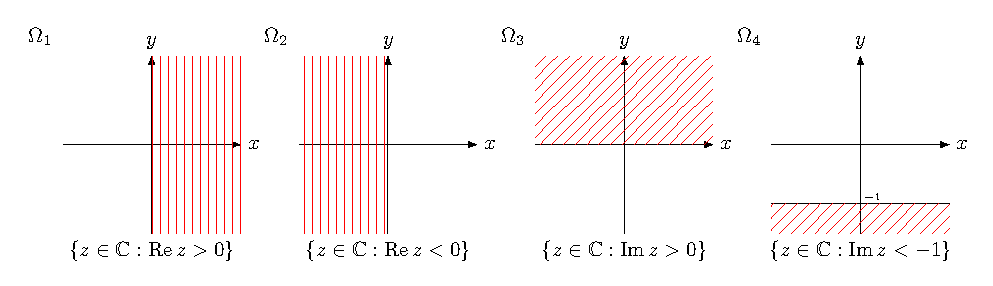
\includegraphics[width=\textwidth]{image_graph1.pdf}

    
\includegraphics{img_graph2.pdf}

    
\includegraphics{img_graph3.pdf}
% \end{align*}
$\{z \in \mathbb{C}: \text{Re } z > 0\} \quad \{z \in \mathbb{C}: \text{Re } z < 0\} \quad \{z \in \mathbb{C}: \text{Im } z > 0\} \quad \{z \in \mathbb{C}: \text{Im } z < -1\}$

But it is not analytic in $\Omega_6$, since $\partial \in \{z \in \mathbb{C}: |z| < 1\}$ and $f$ is not defined at $z = 0$.

$\{z \in \mathbb{C}: |z| > 1\} \quad \{z \in \mathbb{C}: |z| < 1\}$
\end{example}

Note: $f$ is analytic on a domain $\Omega \iff u$ and $v$ are differentiable on $\Omega$ and CR equations hold.

Exercise (Ex 9.3) The function $f(z) = e^x \cos y + ie^x \sin y = e^z$ is entire.

In the next example: a function for which CR equations hold on the whole plane, but $u$ and $v$ are \emphw{not} differentiable on the whole plane, thus the function is \emphic{not}{} entire.

\begin{example}\label{example:9.4}
\[ 
f(z) = \begin{cases}
e^{-1/z^4} & z \neq 0 \\
0 & z = 0
\end{cases}
\text{ defined everywhere in } \mathbb{C} 
\]

\checkthis CR equations hold for every $z \in \mathbb{C}$.
\end{example}
Claim:
\begin{claim} $f(z)$ is not continuous at $z = 0$ ($\implies$ not differentiable).

    \begin{proof}
 Compute $\lim_{z \to 0} f(z)$ on the path $y = x$:
\[ \lim_{\substack{x \to 0 \\ y = x}} e^{-\frac{1}{(x+iy)^4}} = \lim_{x \to 0} e^{-\frac{1}{(1+i)^4 x^4}} = \lim_{x \to 0} e^{\frac{1}{4x^4}} = +\infty \]
$(1 + i)^4 = (\sqrt{2})^4 (\cos(\frac{\pi}{4}) + i\sin(\frac{\pi}{4})) = -4$ De Moivre.
    \end{proof}
\end{claim}
Next proposition is analogous to propositions about the limits, continuity, and differentiability.

\subsection{Properties of analytic functions}

\begin{proposition}\label{proposition:7.1} If $f, g$ are analytic functions on a domain $\Omega$, then also $f + g$ and $f \cdot g$ are analytic on $\Omega$. If $g(z) \neq 0$ on $\Omega$, then $\frac{f}{g}$ is analytic on $\Omega$. The composition $(g \circ f)$ of two analytic functions on $\Omega$ is an analytic function on $\Omega$.

\begin{proof} \emphi{EXERCISE} \end{proof}
\end{proposition}
\begin{example}\label{example:9.5}
    Prove: if $f(z)$ is analytic and real on a domain $\Omega$, then $f$ is a constant function.

\begin{proof} $f$ is analytic and real on $\Omega \implies f(x,y) = u(x,y) + i \cdot 0$, namely $v(x,y) = 0$; CR equations hold for every $z \in \Omega$.
$f$ from analyticity on $\Omega$: $\frac{\partial u}{\partial x} = \frac{\partial v}{\partial y} = 0$ and 
$\frac{\partial u}{\partial y} = -\frac{\partial v}{\partial x} = 0 \implies u(x,y) = c \in \mathbb{R} \implies f(x,y) = c$, namely $f$ is a constant function.
\end{proof}
\end{example}
\begin{proposition} \label{proposition:7.2}
    If $f$ is analytic on a domain $\Omega$ and $f'(z) = 0$ for all $z \in \Omega$, then $f$ is constant on $\Omega$.

\begin{remark}
     Prop 7.2 is false if $\Omega$ is not connected - $f$ can take different constants (constant values) on each connected component of $\Omega$.
\end{remark}
\begin{proof}
    The version of this proposition for real functions is proved using the Mean Value Theorem, 
    that asserts that under appropriate continuity assumption for $f: (a,b) \to \mathbb{R}$ there exists $c \in (a,b)$ s.t. $f(b) - f(a) = f'(c)(b-a)$. 
    So, if $f'(x) = 0$ for all $x \in (a,b)$, then $f(b) = f(a)$. The problem in the complex case is that there is no analogous idea of "between $a$ and $b$" in $\mathbb{C}$, 
    since there are many routes from $a$ to $b$.

    
\includegraphics{img_graph4.pdf}

However, we can use the Mean Value Theorem for Re $f$ and Im $f$ as follows:

Since $f'(z) = 0$ for all $z \in \Omega$ by CR equations $0 = f'(z) = \frac{\partial u}{\partial x} + i\frac{\partial v}{\partial x}$ for all $z \in \Omega \implies \frac{\partial u}{\partial x} = \frac{\partial u}{\partial y} = \frac{\partial v}{\partial x} = \frac{\partial v}{\partial y} = 0$ for all $z \in \Omega$.
\end{proof}

\begin{claim} $u$ is a constant function.
    \begin{proof}
        We have $u: \Omega \to \mathbb{R}, \frac{\partial u}{\partial x} = \frac{\partial u}{\partial y} = 0$ for all $(x,y) \in \Omega$. Pick $(x_0, y_0), (x_1, y_1) \in \Omega$. $\Omega$ is connected, 
        thus by Def~\ref{definition:4.2} any 2 points in $\Omega$ can be connected by a path that is entirely in $\Omega$. 
        We join $(x_0, y_0)$ and $(x_1, y_1)$ by a path comprised of pieces parallel to $x$-axis or 
        $y$-axis [One needs to show that such path exists!] 
        Since $\frac{\partial u}{\partial x} = 0$ by the Mean Value Theorem, $u$ is constant on the horizontal pieces. In the same way,
        since $\frac{\partial u}{\partial y} = 0$, $u$ is constant on vertical pieces. Thus, $u$ is constant on $\Omega$.
        By a similar argument we obtain that $v$ is constant on $\Omega$, therefore $f = u + iv$ is constant on $\Omega$.
    \end{proof}
\end{claim}
\end{proposition}


\includegraphics{img_graph5.pdf}

Now we are going to study analyticity of multi-valued functions - here we will see the big difference between the complex and real functions.

\section{Analyticity of multi-valued functions}

\subsection{Branch points and branches}
We have seen that analytic function is always continuous, thus multi-valued functions are not analytic as is. The question is: can we choose a branch of such function that is single-valued and analytic?

\begin{definition}\label{definition:8.1} We say that on a domain $\Omega$ there is a single-valued 
    branch of multi-valued function if for every point of $\Omega$ we can choose one of the values of a function such that the resulting single-valued function is continuous in $\Omega$.
\end{definition}

In other words: to choose single-valued branch means to choose the domain of definition of a function such that when a point $z$ 
moves along some closed continuous curve that is contained in the domain of definition and goes back to the starting point we get the same value of the function.

Let us demonstrate how we do that on the following example.

\begin{example}\label{example:10.1} 
    Consider double-valued function $f(z) = \sqrt{z - z_0}$. $f(z)$ is defined for all $z \in \mathbb{C}$. Write: $z - z_0 = r(\cos \theta + i\sin \theta), r = |z - z_0|, \theta = \arg(z - z_0)$.

At every $z \neq z_0$, $f(z)$ attains 2 values ($\implies$ double-valued!).
\begin{align*}
    w_0 &= \sqrt{r}\left(\cos \frac{\theta}{2} + i\sin \frac{\theta}{2}\right) \\
    w_1 &= \sqrt{r}\left(\cos\left(\frac{\theta}{2} + \pi\right) + i\sin\left(\frac{\theta}{2} + \pi\right)\right) = -\sqrt{r}\left(\cos \frac{\theta}{2} + i\sin \frac{\theta}{2}\right) = -w_0
\end{align*}

Let us follow the value $w_0$ when $z$ is on the closed continuous curve $L$ that encircles $z_0$ counterclockwise (anti-clockwise; the positive direction).

If $z$ moves to $z_1$, the argument of $z_1 - z_0$ will be
$\arg(z_1 - z_0) = \theta + \theta_1$.


\includegraphics{img_graph6.pdf}

If it continues to move along $L$, $z$ will eventually return to the starting point: the modulus $r = |z - z_0|$ will be the same, 
but the argument will increase by $2\pi$ (since we completed the circle), and $w_0$ will attain the new value $w_1$.
\begin{align*} 
    w_{new} & = \sqrt{r}\left(\cos\left(\frac{\theta + 2\pi}{2}\right) + i\sin\left(\frac{\theta + 2\pi}{2}\right)\right) \\ 
            & = \sqrt{r}\left(\cos\left(\frac{\theta}{2} + \pi\right) + i\sin\left(\frac{\theta}{2} + \pi\right)\right) = w_1 = -w_0 
\end{align*}

Let us check what happens to $w_0$ is we move along a closed continuous curve that does not encircle the point $z_0$.
\end{example}


\includegraphics{img_graph7.pdf}

From the picture above that the value of the modulus and of the argument after completing the full circle will return to its starting value - the same, with no change. 
This is independent of the curve $L_1$ (the only important thing that the curve does not encircle the point $z_0$).
\begin{corollary}\label{corollary:8.1} 
    On a domain $\Omega$ that contains curves that encircle $z_0$, it is impossible to choose a continuous branch of the function $\sqrt{z - z_0}$.
\end{corollary}

% \section*{Lecture Notes,Lectures 11 + 12}
\lecture{11+12}{Continuation and Harmonic functions}

We have studied the double-valued function \( f(z) = \sqrt{z - z_0} \).

Reference, corollary \ref{corollary:8.1}.

For example: On \( \frac{1}{2} < |z - z_0| < 2 \), it is impossible to choose a single-valued branch of \( \sqrt{z - z_0} \).

On \( |z - z_0| > 1 \), it is impossible to choose a single-valued branch of \( \sqrt{z - z_0} \).

We have also seen that if the curve does not encircle \( z_0 \), then the value of \( \sqrt{z - z_0} \) stays the same. 
So, we have another corollary.

\begin{corollary}\label{corollary:8.2}
    It is possible to choose a single-valued branch of the function \( \sqrt{z - z_0} \) on a domain \( \Omega \) 
    if none of the closed continuous curves in \( \Omega \) encircle \( z_0 \).
\end{corollary}

Intuitively, if we would be able to "cut" the plane (in some way) up to \( z_0 \), including \( z_0 \), then there will be no closed curve that encircles \( z_0 \).
Indeed, the biggest domain on which none of the closed continuous curves encircle \( z_0 \) is the cutted plane, where we cut as follows.

\subsection*{The "largest" such domain}
\begin{itemize}
    \item Cut-plane: \( \mathbb{C} \) without the line \( \{ z = x + iy \mid x \leq x_0 \} \) 
    (including \( z_0 \)).
    
    
\includegraphics{img_graph8.pdf}

    \item Cut-plane: two single-valued branches:
    \[
        w_0 = \sqrt{r} (\cos \frac{\theta}{2} + i \sin \frac{\theta}{2}), \quad 
        w_1 = -\sqrt{r} (\cos \frac{\theta}{2} + i \sin \frac{\theta}{2})
    \]

    
\includegraphics{img_graph9.pdf}
\end{itemize}

\emphOnly{Note}: We can cut along any ray starting at \( z_0 \).

The cut will prevent any closed curve from encircling \( z_0 \). In the case of the line in the picture above (ray creates an angle \( \theta \) with the positive counterclockwise direction with the \( x \)-axis), we have:

For a ray with \( \theta = \frac{\pi}{4} \), two continuous branches of \( \sqrt{z - z_0} \):

\[
    w = \pm \sqrt{r} (\cos \frac{\theta}{2} + i \sin \frac{\theta}{2}), \quad \frac{\pi}{4} < \theta \leq \frac{5\pi}{4}
\]

\begin{definition}\label{definition:8.2} The point \( z_0 \) is called a \textit{branch point} for a complex multi-valued function if the value of \( f(z) \) does not return to its initial value as a closed curve around the point is traced (starting from some arbitrary point on the curve) in such a way that \( f \) varies continuously as the path is traced.
\end{definition}
\textbf{Important:} What matters here is the \textbf{local} behavior of the function \( f \) near \( z_0 \). What may happen on paths that are some distance away from \( z_0 \) is not relevant. To be more precise:

\noindent \textbf{The behavior must occur for all the curves that enclose the point and are sufficiently close to it.}

In example \ref{example:10.1} \( z = z_0 \) is the \textbf{Branch Point}.

Let us consider a more general case.


\begin{example} Consider \( w = \sqrt[n]{z - z_0} \). Take \( z - z_0 = r (\cos \theta + i \sin \theta) \). Then:

\[
w_k = \sqrt[n]{r} \left( \cos \frac{\theta + 2\pi k}{n} + i \sin \frac{\theta + 2\pi k}{n} \right), \quad k = 0,1,2, \dots, n-1.
\]

Fix \( 0 \leq k_0 \leq n-1 \).

As before, we let \( z \) be on the closed continuous curve \( L \) that encloses \( z_0 \). 


\includegraphics{img_graph10.pdf}

When \( z \) will complete the full circle (anticlockwise), the modulus \( r \) will return to the same value. The argument, however, will increase by \( 2\pi \), and \( w \) will attain a new value.
% \end{example}
\emphic{After full circle around $z_0 $:}{}
\[
w = \sqrt[n]{r} \left( \cos \frac{(\theta + 2\pi) + 2\pi k_0}{n} + i \sin \frac{(\theta + 2\pi) + 2\pi k_0}{n} \right).
\]

\[
= \sqrt[n]{r} \left( \cos \frac{\theta + 2\pi k_0}{n} + i \sin \frac{\theta + 2\pi k_0}{n} \right) 
\cdot \left( \cos \frac{2\pi}{n} + i \sin \frac{2\pi}{n} \right).
\]

\[
= w_{k_0} \left( \cos \frac{2\pi}{n} + i \sin \frac{2\pi}{n} \right) = w_{k_0 + 1}.
\]
\end{example}

Namely, the new value of \( w \) is equal to the previous one times \( \left( \cos \frac{2\pi}{n} + i \sin \frac{2\pi}{n} \right) \).

\checkthis{}

\[
\left( \cos \frac{2\pi}{n} + i \sin \frac{2\pi}{n} \right)^n = 1.
\]

This is independent of the curve that encloses \( z_0 \). If \( z \) runs on a curve that does not encircle \( z_0 \), then, as before, the value \( w_{k_0} \) will not change once \( z \) returns to the starting point.

\textbf{Conclusion:} If \( z \) is on the curve that encloses \( z_0 \) once (anticlockwise), then the value \( \sqrt[n]{z - z_0} = w_{k_0} \) will change to the new value \( w_{k_0 + 1} \). If \( z \) is on the curve that does not enclose \( z_0 \), 
then the value of the function stays the same.
$\implies z = z_0$ is the branch point of the function $f(z) = \sqrt[n]{z - z_0}$.

\begin{example}\label{example:10.3} Find the branch points of the function $f(z) = \sqrt{1 + z^2}$.
    \begin{soln}
        $\sqrt{1 + z^2} = \sqrt{z - i} \cdot \sqrt{z + i}$, therefore $z = \pm i$ are the branch points of $\sqrt{z - i}$, $\sqrt{z + i} \implies$ branch points of $\sqrt{1 + z^2}$.
Let us see on the picture what happens and where to cut so we will be able to obtain a continuous single-valued branch of $f(z)$.

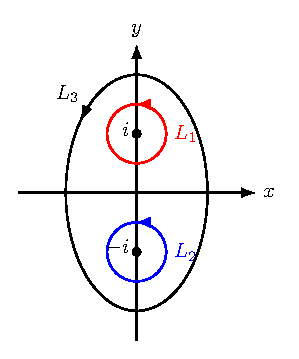
\includegraphics{img_graph11.pdf}

If $z$ is on $L_1$ (around $z = i$): when $z$ returns to the initial point $\sqrt{z + i}$ returns to the same value since $L_1$ does not enclose $z = -i$ while $\sqrt{z - i}$ attains new value - changes the sign of the previous one. Therefore, $f(z)$ also changes the sign. In the same way: if $z$ is on $L_2$, then upon return to the initial point $\sqrt{z + i}$ will change the value - change the sign, $\sqrt{z - i}$ will return to the same value, and the function will change the sign. If $z$ is on $L_3$ that encloses both $z_0 = i$ and $z_0 = -i$, then $\sqrt{z - i}$ and $\sqrt{z + i}$ will change the sign, but their product - the original function - will not!
    \end{soln}
\end{example}

$\implies$ We can choose a continuous branch on a domain $\Omega$ if none of the closed curves in $\Omega$ enclose $i$ and not $-i$ (or $-i$ and not $i$), but it can enclose both. Namely, if we cut the plane along the interval connecting $i$ and $-i$, we will get a domain in which it is possible to choose a continuous branch.

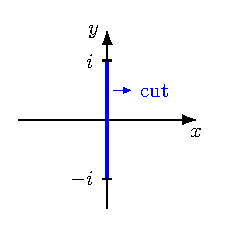
\includegraphics{img_graph12.pdf}

\begin{definition}\label{definition:8.3} Single-valued branch is called an analytic function on a domain $\Omega$ if it is differentiable at every $z \in \Omega$.
\end{definition}

\begin{example}\label{example:10.4} Prove that $w = \sqrt[n]{z}$ is analytic on the domain $\Omega = \{z \in \mathbb{C}: 0 < \arg z < \frac{2\pi}{n}\}$.

\begin{proof}    We have already seen that on the cut-plane with the cut
along any ray starting at $z_0 = 0$ (including $z_0 = 0$) every branch of this function is single-valued and continuous. Let us prove that it is differentiable and find the derivative.

\begin{align*}  & \frac{f(z) - f(z_0)}{z - z_0} = \frac{(f(z))^n - (f(z_0))^n}{z - z_0} \\ 
                & = \frac{1}{(\sqrt[n]{z})^n - (\sqrt[n]{z_0})^n} \cdot \frac{(f(z))^{n-1} + (f(z))^{n-2}f(z_0) + \dots + (f(z_0))^{n-1}}{z - z_0} \\
                & = \frac{1}{(\sqrt[n]{z})^{n-1} + (\sqrt[n]{z})^{n-2}\sqrt[n]{z_0} + \dots + (\sqrt[n]{z_0})^{n-1}} \end{align*}

Now we pass to the limit as $z$ tends to $z_0$ and obtain
\[ \implies \lim_{z \to z_0} \frac{f(z) - f(z_0)}{z - z_0} = \frac{1}{n(\sqrt[n]{z_0})^{n-1}} \]
$\implies f$ is differentiable and \[ (\sqrt[n]{z})' = \frac{1}{n(\sqrt[n]{z})^{n-1}}.\]
\end{proof}
\end{example}

In many problems in hydrodynamics, the elasticity theory and other fields there is often a need to recreate an analytic function from its real part. Now we will find the set of functions for which it is possible. Our subject is:

\section{Harmonic functions.}

\subsection{Definitions and basic results}

\begin{definition}\label{definition:9.1} The real function $u(x,y)$ is called harmonic on a domain $\Omega$ if it is continuous on $\Omega$ with continuous partial derivatives of the first and second order 
    \[\{\frac{\partial u}{\partial x}, \frac{\partial u}{\partial y}, \frac{\partial^2 u}{\partial x^2}, \frac{\partial^2 u}{\partial y^2}, \frac{\partial^2 u}{\partial x \partial y}, \frac{\partial^2 u}{\partial y \partial x}\},\] and the following equation, called the Laplace equation, holds:
\[ \frac{\partial^2 u}{\partial x^2} + \frac{\partial^2 u}{\partial y^2} = 0 \]
\end{definition}

\begin{example}\label{example:11.1} The function $u(x,y) = x^2 - y^2$ is harmonic for every $(x,y) \in \mathbb{R}^2$.
\begin{soln}
         $u(x,y)$ is defined everywhere, and we have:
    $\frac{\partial u}{\partial x} = 2x \quad \frac{\partial u}{\partial y} = -2y \quad \frac{\partial^2 u}{\partial x^2} = 2 \quad \frac{\partial^2 u}{\partial y^2} = -2 \quad \frac{\partial^2 u}{\partial x \partial y} = \frac{\partial^2 u}{\partial y \partial x} = 0$
    
    All partial derivatives are continuous everywhere, and $\frac{\partial^2 u}{\partial x^2} + \frac{\partial^2 u}{\partial y^2} = 2 + (-2) = 0$.
\end{soln}
\end{example}

\begin{example}\label{example:11.2} The function $u(x,y) = e^x y$ is \textbf{not} harmonic function on $\mathbb{R}^2$.
\begin{proof} $u(x,y)$ is defined everywhere on $\mathbb{R}^2$.

\begin{align*}
    & \frac{\partial u}{\partial x} = ye^{xy} \qquad & \frac{\partial u}{\partial y} &= xe^{xy} \\ 
    & \frac{\partial^2 u}{\partial x^2} = y^2e^{xy} \qquad & \frac{\partial^2 u}{\partial y^2} &= x^2e^{xy} \\
    & \frac{\partial^2 u}{\partial x \partial y} = e^{xy} + yxe^{xy} \qquad & \frac{\partial^2 u}{\partial y \partial x} &= e^{xy} + xye^{xy} 
\end{align*}

All partial derivatives are defined and continuous for all $(x,y) \in \mathbb{R}^2$. However $\frac{\partial^2 u}{\partial x^2} + \frac{\partial^2 u}{\partial y^2} = y^2e^{xy} + x^2e^{xy} = e^{xy}(x^2 + y^2) \neq 0$ except for $(0,0) \implies u(x,y)$ is \textbf{not} harmonic function on $\mathbb{R}^2$.
\end{proof}
\end{example}

\begin{proposition}\label{proposition:9.1} If the function $f(z) = u(x,y) + iv(x,y)$ is analytic on a domain $\Omega$, then $u(x,y)$ and $v(x,y)$ are harmonic on $\Omega$.
\end{proposition}

    \begin{proof}
By CR equations $\frac{\partial u}{\partial x} = \frac{\partial v}{\partial y}$ and $\frac{\partial u}{\partial y} = -\frac{\partial v}{\partial x}$ (since $f$ is analytic). Let us differentiate the first equation with respect to $x$ and the second with respect to $y$:
\[ \frac{\partial^2 u}{\partial x^2} = \frac{\partial^2 v}{\partial y \partial x}, \quad \frac{\partial^2 u}{\partial y^2} = -\frac{\partial^2 v}{\partial x \partial y} \]
Since $f$ is analytic, $u$ and $v$ are continuously differentiable, thus from theory of real functions, we know that $\frac{\partial^2 v}{\partial y \partial x} = \frac{\partial^2 v}{\partial x \partial y}$. Therefore, if we add the equations (*), we obtain:
\[ \frac{\partial^2 u}{\partial x^2} + \frac{\partial^2 u}{\partial y^2} = \frac{\partial^2 v}{\partial y \partial x} - \frac{\partial^2 v}{\partial x \partial y} = \frac{\partial^2 v}{\partial x \partial y} - \frac{\partial^2 v}{\partial x \partial y} = 0 \]
$\implies u$ is harmonic function on $\Omega$.

If we differentiate now $\frac{\partial u}{\partial x} = \frac{\partial v}{\partial y}$ with respect to $y$ and $\frac{\partial u}{\partial y} = -\frac{\partial v}{\partial x}$ with respect to $x$, and use $\frac{\partial^2 u}{\partial x \partial y} = \frac{\partial^2 u}{\partial y \partial x}$ we will obtain that $v$ is also harmonic function on $\Omega$.
    \end{proof}

This proposition implies that in order to construct an analytic function we cannot choose the real and imaginary parts in an arbitrary way. The functions that we choose must be harmonic and, moreover, the CR equations must hold.

\begin{definition}\label{definition:9.2} If $u(x,y)$ and $v(x,y)$ are harmonic functions on a domain $\Omega$ such that CR equations hold ($\frac{\partial u}{\partial x} = \frac{\partial v}{\partial y}, \frac{\partial u}{\partial y} = -\frac{\partial v}{\partial x}$), then the function $v(x,y)$ is called the \emphw{harmonic conjugate} of the function $u(x,y)$ on a domain $\Omega$.
\end{definition}
\begin{proposition}\label{proposition:9.2} The function $f(z) = u(x,y) + iv(x,y)$ is analytic in a domain $\Omega \iff v(x,y)$ is the harmonic conjugate of $u(x,y)$.
\end{proposition}

\begin{proof} [$\implies$] Assume $f$ is analytic in a domain $\Omega$. By Prop~\ref{proposition:9.1}
$u(x,y)$ and $v(x,y)$ are harmonic functions on $\Omega$. Since $f$ is analytic, CR equations hold, thus by Def~\ref{definition:9.2} $v(x,y)$ is the harmonic conjugate of $u(x,y)$.

[$\impliedby$] If $u(x,y)$ and $v(x,y)$ are harmonic functions on a domain $\Omega$, then $u$ and $v$ are differentiable at all $z \in \Omega$. Since $v(x,y)$ is the harmonic conjugate of $u(x,y)$, 
by Def~\ref{definition:9.2} - CR equations hold, 
thus Thm 6.1 \ref{theorem:6.1} asserts that $f$ is analytic in a domain $\Omega$.
\end{proof}

Thus, to conclude that we can reconstruct an analytic function from its real part we need to know whether it is always possible to find a harmonic conjugate to a given harmonic function. The answer is yes - it is given by the following proposition which we state without the proof.

\begin{proposition}\label{proposition:9.3} For any harmonic function $u(x,y)$ in a domain $\Omega$ there exists a function $v(x,y)$ in $\Omega$ which is the harmonic conjugate of $u(x,y)$.

The proof is by construction: one explicitly constructs the function $v(x,y)$. Since the proof involves somewhat complicated real analysis, we omit it.
\end{proposition}

\begin{example}\label{example:11.3} Find an analytic function $f(z) = u(x,y) + iv(x,y)$ such that $u(x,y) = \text{Re } f(z) = \arctan \frac{y}{x}$.

\begin{soln} Let us compute the partial derivatives and then use CR equations: Recall: $(\arctan x)' = \frac{1}{1 + x^2}$
\[ \frac{\partial u}{\partial x} = \frac{-y}{x^2 + y^2} \qquad \frac{\partial u}{\partial y} = \frac{x}{x^2 + y^2} \implies \frac{\partial v}{\partial y} = \frac{-y}{x^2 + y^2}, \frac{\partial v}{\partial x} = \frac{-x}{x^2 + y^2} \]
CR equations

To obtain $v(x,y)$ we integrate $\frac{\partial v}{\partial x}$ with respect to $x$ (or $\frac{\partial v}{\partial y}$ with respect to $y$).
\[ v(x,y) = \int \frac{\partial v}{\partial x} dx = \int \frac{-x}{x^2 + y^2} dx = -\frac{1}{2} \ln(x^2 + y^2) + c(y) \]
Since the integral is with respect to $x$, the constant may depend on $y$ (only!) To find $c(y)$ we differentiate $v(x,y)$ in (*) with respect to $y$ and compare it to $\frac{\partial v}{\partial y}$ obtained from CR equations:
\[ \frac{\partial v}{\partial y} = \frac{-y}{x^2 + y^2} + c'(y) = \frac{-y}{x^2 + y^2} \implies c'(y) = 0 \implies c = \text{constant} \in \mathbb{R} \]
$\implies v(x,y) = -\frac{1}{2}\ln(x^2 + y^2) + c$ and $f(z) = \arctan \frac{y}{x} - \frac{i}{2}[\ln(x^2 + y^2) + 2c]$.

\end{soln}
\end{example}
% %\usepackage{xr}

% \externaldocument{note01}
% \externaldocument{note02}
% \externaldocument{note03}
% \externaldocument{note04}
% \externaldocument{note05}
% \externaldocument{note06}
% \externaldocument{note07}
% \externaldocument{note08}
% \externaldocument{note09}
% \externaldocument{note10}
% \externaldocument{note11}

\graphicspath{{./input/graphs/note05/}}


% \zexternaldocument{note01}
% \zexternaldocument{note02}
% \zexternaldocument{note03}
% \zexternaldocument{note04}
% \zexternaldocument{note05}
% \zexternaldocument{note06}
% \zexternaldocument{note07}
% \zexternaldocument{note08}
% \zexternaldocument{note09}
% \zexternaldocument{note10}
% \zexternaldocument{note11}
% \externaldocument{note12}



\week{5}
% \section*{Week 5. Lecture 13.}
\lecture{13}{Sequences in $\mathbb{C}$}
We introduce complex sequences and series, discuss their convergence and use them to construct complex power series. Then, we make several concrete connections with complex differentiable functions.

\section{Complex sequences.}

\subsection{Sequence limits}

\begin{definition}\label{definition:10.1} A sequence $\{z_n\}_{n=0}^{\infty}, z_n \in \mathbb{C}$, has limit $z$ (as $n \to \infty$) if for every $\epsilon > 0$ there exists $N = N(\epsilon) \in \mathbb{N}$ such that for all $n > N$, $|z_n - z| < \epsilon$. Notation: $\lim_{n \to \infty} z_n = z$.
\end{definition}
If the limit does not exist (or $\infty$), we say that the sequence diverges.

In other words, a sequence of complex numbers $\{z_n\}$ converges to the complex number $z$ iff at every neighborhood of $z$ there are almost all but finite number of points from the sequence: $\lim_{n \to \infty} z_n = z \iff \forall \epsilon > 0 \quad \exists N(\epsilon) \in \mathbb{N} \text{ s.t. for every } n > N(\epsilon) \quad |z_n - z| < \epsilon$.

\begin{claim}
If $\lim_{n \to \infty} z_n$ exists, then it is unique.
\begin{proof}
Assume $\lim_{n \to \infty} z_n = \tilde{z_1}$ and $\lim_{n \to \infty} z_n = \tilde{z_2}$. Then, for any $\epsilon > 0$ there exists $N_1 \in \mathbb{N}$ s.t. 
for every $n > N_1$, $|z_n - \tilde{z_1}| < \epsilon/2$. Also there exists $N_2 \in \mathbb{N}$ s.t. for every $n > N_2$, $|z_n - \tilde{z_2}| < \epsilon/2$. 
Choose $N = \max\{N_1, N_2\}$, then for every $n > N$, $|z_n - \tilde{z_1}| < \epsilon/2$ and $|z_n - \tilde{z_2}| < \epsilon/2$.

Thus $|\tilde{z_1} - \tilde{z_2}| = |\tilde{z_1} - z_n + z_n - \tilde{z_2}| \leq |\tilde{z_1} - z_n| + |z_n - \tilde{z_2}| < \epsilon/2 + \epsilon/2 = \epsilon$. Since this is true for any $\epsilon > 0$ we conclude that $\tilde{z_1} = \tilde{z_2}$.
\end{proof}
\end{claim}
Also, it is possible to show that the complex sequence $\{z_n\}$ converges to $z \iff$ the real sequence $\{|z_n - z|\}_{n=0}^{\infty}$ converges to 0 (\verifythis)

\begin{example}\label{example:12.1} Let $z_n = (\frac{i}{2})^n, n \in \mathbb{N}$. Then: $z_0 = 1, z_1 = \frac{i}{2}, z_2 = \frac{i^2}{4} = -\frac{1}{4}, z_3 = \frac{i^3}{8} = -\frac{i}{8}, z_4 = \frac{i^4}{16} = \frac{1}{16}, \dots$
\end{example}
This sequence converges to 0: $\lim_{n \to \infty} z_n = 0$. Can be demonstrated by proving that $|z_n|$ decreases to 0 as $n$ tends to infinity. (\checkthis{} By graphing the points $z_n$ check that the sequence
$\{z_n\}$ "spirals" in toward the origin $(0)$ in the $z$-plane.

\begin{example}\label{example:12.2} Let $z_n = (2i)^n: z_0 = 1, z_1 = 2i, z_2 = -4, z_3 = -8i, \dots$. This sequence diverges: one can show that $\{|z_n|\}_{n=0}^{\infty}$ is unbounded increasing sequence \{namely, $|z_n|$ gets arbitrarily large\}.
\end{example}

\begin{example}\label{example:12.3} Let $z_n = (i)^n: z_0 = 1, z_1 = i, z_2 = -1, z_3 = -i, z_4 = 1, z_5 = i, \dots$. This is a bounded sequence ($|z_n| \leq 1$ for any $n$), but $\lim_{n \to \infty} z_n$ does not exist: there is no $z$ such that almost all but finitely many points of the sequence are in a small neighborhood of some $z$: 
    
    
\includegraphics{img_graph1.pdf}
    
    $z_n$ jumps at every step.
\end{example}

Important real sequence (limit): let $a_n = (1 + \frac{a}{n})^n$ for some $a$. Then $\lim_{n \to \infty} a_n = (1 + \frac{a}{n})^n = e^a$.

\begin{example}\label{example:12.4} $\lim_{n \to \infty} (1 + \frac{i}{n})^n = e^i, \quad \lim_{n \to \infty} (1 - \frac{i}{n})^n = \lim_{n \to \infty} (1 + \frac{-i}{n})^n = e^{-i} = \frac{1}{e^i}$.
\end{example}

\begin{proposition} \zlabel{proposition:10.1} 
    If the sequences $\{z_n\}, \{w_n\}$ of complex numbers converge, then so the sequences $\{z_n \pm w_n\}, \{z_n \cdot w_n\}$, 
    and if $w_n \neq 0$ also $\{\frac{z_n}{w_n}\}$, and 
    \[\lim_{n \to \infty} (z_n \pm w_n) = \lim_{n \to \infty} z_n \pm \lim_{n \to \infty} w_n; \quad \lim_{n \to \infty} z_n w_n = \lim_{n \to \infty} z_n \lim_{n \to \infty} w_n.\]

If $\lim_{n \to \infty} w_n \neq 0$, then: $\lim_{n \to \infty} \frac{z_n}{w_n} = \frac{\lim_{n \to \infty} z_n}{\lim_{n \to \infty} w_n}$.
\end{proposition}

\section{Complex (scalar) series.}

\subsection{Series convergence}

\begin{definition}\label{definition:11.1} 
    The complex (scalar) series $\sum_{n=1}^{\infty} z_n$ converges to the value $s \in \mathbb{C}$ if the sequence of partial sums $\{S_N\}_{N=0}^{\infty}, S_N = z_0 + z_1 + \dots + z_N$ converges to $s$. 
    The value $s$ is called the sum of the series. If the limit does not exist (or $\infty$) ($\lim_{N \to \infty} S_N$) then the series diverges. If the series converges to some value $s$, then $s$ is unique.
\end{definition}

\begin{remark}
Furthermore: if $r_N = S - S_N = \sum_{n=N+1}^{\infty} z_n$, then it is possible to show that $\sum_{n=0}^{\infty} z_n = S \iff \lim_{N \to \infty} r_N = 0$. 
Namely, the \emphi{tail} of the series converges to 0.
\end{remark}
From Def (\ref{definition:11.1}) we immediately conclude:
\begin{proposition}\label{proposition:11.1} If $\sum_{n=0}^{\infty} z_n$ converges, then $\lim_{n \to \infty} z_n = 0$.
\begin{proof}
    By Def (\ref{definition:11.1}): If $\sum_{n=0}^{\infty} z_n = S$, then $\lim_{N \to \infty} S_N = \lim_{N \to \infty} \sum_{n=0}^{N} z_n = S$. On the other hand: $S_N - S_{N-1} = (z_0 + z_1 + \dots + z_N) - (z_0 + z_1 + \dots + z_{N-1}) = z_N$
    $\implies \lim_{N \to \infty} z_N = \lim_{N \to \infty} (S_N - S_{N-1}) = \lim_{N \to \infty} S_N - \lim_{N \to \infty} S_{N-1} = S - S = 0$ by Prop 10.1(\zref{proposition:10.1}). $s$ is unique.
\end{proof}
\end{proposition}
The contrapositive statement is often called the Test for Divergence.

\begin{proposition}[Test for Divergence]\label{proposition:11.2} (Test for Divergence) Let $\{z_n\}_{n=0}^{\infty} \in \mathbb{C}$. If $\lim_{n \to \infty} z_n \neq 0$ (or does not exist), then the series $\sum_{n=0}^{\infty} z_n$ diverges.
\end{proposition}

\begin{remark}
The converse of Prop 11.2(\ref{proposition:11.2}) is false: $\lim_{n \to \infty} \frac{1}{n} = 0$, but the series $\sum_{n=1}^{\infty} \frac{1}{n}$ diverges!
\end{remark}
As expected there is an immediate relation between convergence or divergence of complex sequences and series to that of real ones.

\begin{proposition}\label{proposition:11.3} Let $\{z_n\}_{n=0}^{\infty}, z_n$ be the complex sequence and the complex series. Suppose that $z = x + iy$ and $S = u + iv$. Then:
\begin{enumerate}
    \item $\lim_{n \to \infty} z_n = z \iff \lim_{n \to \infty} x_n = x$ and $\lim_{n \to \infty} y_n = y$ (for $z_n = x_n + iy_n$)
    \item $\sum_{n=0}^{\infty} z_n = S \iff \sum_{n=0}^{\infty} x_n = u$ and $\sum_{n=0}^{\infty} y_n = v$
\end{enumerate}
\begin{proof}
    \begin{enumerate}
        \item follows directly from Def 10.1(\ref{definition:10.1}) and the application of triangle inequality: $|x_n - x|, |y_n - y| \leq |z_n - z| \leq |x_n - x| + |y_n - y|$
        \item is proved by decomposing the complex sum into real and imaginary parts $\sum_{n=0}^{\infty} z_n = \sum_{n=0}^{\infty} x_n + i\sum_{n=0}^{\infty} y_n$ and a careful use of 1) [FINISH!]
    \end{enumerate}
\end{proof}
\end{proposition}

Hint: If $\sum_{n=0}^{\infty} x_n = u, \sum_{n=0}^{\infty} y_n = v \implies$ obvious. Assume $\sum_{n=0}^{\infty} z_n = S$, define $X_N = \sum_{n=0}^{N} x_n, Y_N = \sum_{n=0}^{N} y_n$, apply 1) to $S_N = \sum_{n=0}^{N} z_n$.

In much of what follows, we can use Prop 11.3 and results in real sequences and series - these are left as an exercise. For example, Prop 10.1 and an analogous proposition for the series:

\begin{proposition} \label{proposition:11.4} Suppose that $\sum_{n=0}^{\infty} z_n = S, \sum_{n=0}^{\infty} w_n = t$ are two convergent series. Let $\alpha \in \mathbb{C}$. Then,
\begin{enumerate}
    \item $\sum_{n=0}^{\infty} (z_n \pm w_n) = S \pm t$ (converges to $S \pm t$)
    
    \item $\sum_{n=0}^{\infty} \alpha z_n = \alpha S$ (converges to $\alpha S$)
\end{enumerate}

\begin{proof} (EXERCISE - exactly as in the real case - partial sums).
\end{proof}
\end{proposition}

\begin{example} \label{example:13.1} (Key example - Geometric series)

Suppose that $|z| < 1$. We claim that the series $\sum_{n=0}^{\infty} z^n$, called the Geometric series, converges.
\begin{claim}\label{claim:11.5}
    $\sum_{n=0}^{\infty} z^n$ converges (if $|z| < 1$) and $\sum_{n=0}^{\infty} z^n = \frac{1}{1-z}$.
\end{claim}
\begin{proof}
    We prove it using Def 11.1: we will show that the sequence of partial sums converges to $\frac{1}{1-z}$.
    Need to show: $\lim_{N \to \infty} S_N = \lim_{N \to \infty} \sum_{n=0}^{N} z^n = \frac{1}{1-z}$.
    
    First, we obtain a closed formula for $S_N$ as follows.
    \begin{align*}
        S_N &= 1 + z + z^2 + \dots + z^N \\
        z \cdot S_N &= z + z^2 + z^3 + \dots + z^{N+1} \\
        &\implies S_N - zS_N = S_N(1-z) = 1 - z^{N+1} \\
        &\implies S_N = \frac{1 - z^{N+1}}{1-z}
    \end{align*}
\end{proof}
Now we use this formula to compute the limit
\[ \left| \frac{1}{1-z} - S_N \right| = \left| \frac{1}{1-z} - \frac{1 - z^{N+1}}{1-z} \right| = \left| \frac{z^{N+1}}{1-z} \right| = \frac{|z|^{N+1}}{|1-z|} \]
Since $|z| < 1 \implies \lim_{N \to \infty} |z|^N = 0$ (from what we know about real sequences). Therefore $\left| \frac{1}{1-z} - S_N \right| \xrightarrow{N \to \infty} 0 \implies \lim_{N \to \infty} S_N = \frac{1}{1-z}$.
\end{example}

% \section*{Lectures 14+15.}
\lecture{14+15}{Absolute convergence?! WTH is that?}

Now we introduce the notion of absolute convergence.

\begin{definition}\label{definition:11.2} The series $\sum_{n=0}^{\infty} z_n$ converges absolutely if the series of the moduli of the terms $\sum_{n=0}^{\infty} |z_n|$ converges.
\end{definition}

\begin{remark}
Note: (The Geometric series) For $|z| < 1$, $\sum_{n=0}^{\infty} |z|^n$ converges. Namely, the geometric series converges absolutely.
\begin{proof}
    Follow exactly the same steps as in Ex 13.1, replace $z$ by $|z|$.
\end{proof}
\end{remark}

The definition of absolute convergence is subtle: Series can converge, but not absolutely: $\sum_{n=1}^{\infty} \frac{(-1)^n}{n}$ converges, but $\sum_{n=1}^{\infty} |\frac{(-1)^n}{n}| = \sum_{n=1}^{\infty} \frac{1}{n}$ diverges.

The absolute convergence *however* always implies convergence:

\begin{proposition}\label{proposition:11.6} If $\sum_{n=0}^{\infty} |z_n|$ converges, then $\sum_{n=0}^{\infty} z_n$ converges.
\begin{proof}
    We have $|z_n| = \sqrt{x_n^2 + y_n^2} \geq |x_n|, |y_n|$, therefore using the Comparison test for positive (real) series we get that $\sum_{n=0}^{\infty} |x_n|$ 
    and $\sum_{n=0}^{\infty} |y_n|$ converge $\implies$ (by analogous statement for real series) $\sum_{n=0}^{\infty} x_n$ and $\sum_{n=0}^{\infty} y_n$ converge. 
    Thus, by Prop 11.3(\ref{proposition:11.3}) 2) $\sum_{n=0}^{\infty} z_n$ converges.
\end{proof}
\end{proposition}

Now we state 3 very useful tests for convergence of complex series.

\begin{proposition} \label{proposition:11.7} Let $\sum_{n=0}^{\infty} a_n, a_n \in \mathbb{C}$ be a complex series.

\begin{enumerate}
    \item \textbf{Ratio-Test:} Consider the limit $\lim_{n \to \infty} \left| \frac{a_{n+1}}{a_n} \right| = \lim_{n \to \infty} \frac{|a_{n+1}|}{|a_n|} = L$
    \begin{itemize}
        \item If the limit exists and $L < 1$, then the series $\sum_{n=0}^{\infty} a_n$ converges absolutely.
        \item If the limit exists and $L > 1$, then the series $\sum_{n=0}^{\infty} a_n$ diverges.
        \item If $L = 1$ or the limit does not exist, then the test is inconclusive \{namely, there are examples of convergent and divergent series\}.
    \end{itemize}
    \item \textbf{Root (Cauchy) Test:} Consider the limit $\lim_{n \to \infty} \sqrt[n]{|a_n|} = L$
    \begin{itemize}
        \item If the limit exists and $L < 1$, then the series $\sum_{n=0}^{\infty} a_n$ converges absolutely.
        \item If the limit exists and $L > 1$, then the series $\sum_{n=0}^{\infty} a_n$ diverges.
        \item If $L = 1$ or does not exist, then the test is inconclusive.
    \end{itemize}
    \item \textbf{Comparison Test:}
    \begin{itemize}
        \item If $0 \leq |a_n| < r_n$ and the positive real series $\sum_{n=0}^{\infty} r_n$ converges, then $\sum_{n=0}^{\infty} a_n$ converges absolutely.
        \item If $|a_n| > r_n \geq 0$ and $\sum_{n=0}^{\infty} r_n$ diverges, then $\sum_{n=0}^{\infty} a_n$ diverges.
    \end{itemize}

\end{enumerate}
\end{proposition}
\begin{proof}
    Ratio Test: If $L > 1$, then the sequence $\{|a_n|\}$ is increasing (for sufficiently large $n$), therefore the series diverges by the Test for Divergence.
    
    Suppose that $L < 1$. Choose a number $r$ such that $L < r < 1$. Since $\lim_{n \to \infty} \left| \frac{a_{n+1}}{a_n} \right| = L$ there exists $N \in \mathbb{N}$ such that for all $n \geq N: \left| \frac{|a_{n+1}|}{|a_n|} - L \right| < \epsilon$. Set $\epsilon = a_N$. Then we have $|a_{N+1}| \leq r|a_N| = |a|r$, $|a_{N+2}| \leq r|a_{N+1}| < |a|r^2$ and, in general $|a_{N+k}| \leq |a|r^k$. Therefore for $n \geq N$ the terms of the series $\sum_{n=0}^{\infty} |a_n|$ are bounded by the terms of a convergent geometric series (since $0 \leq r < 1$), therefore $\sum_{n=0}^{\infty} |a_n|$ converges by the Comparison Test (for real series), namely, $\sum_{n=0}^{\infty} a_n$ converges absolutely.
    
    Root Test and Comparison Test: EXERCISE!
\end{proof}

\begin{example}\label{example:13.2} Check the convergence of the following series:
    \begin{enumerate}
        \item  $\sum_{n=0}^{\infty} (2i)^n$ 
        \item  $\sum_{n=0}^{\infty} \left(\frac{1+i}{2}\right)^n$ 
        \item  $\sum_{n=0}^{\infty} \frac{(4i)^n}{n!}$
    \end{enumerate}
\begin{soln}
    \begin{enumerate}
        \item We use Comparison Test as follows: $a_n = (2i)^n \implies |a_n| = (|2i|)^n = |2|^n = 2^n > (\frac{3}{2})^n$. Since $\sum_{n=0}^{\infty} (\frac{3}{2})^n$ diverges (for example, by the Test for Divergence, since $\lim_{n \to \infty} (\frac{3}{2})^n = \infty \neq 0$) by Comparison Test $\sum_{n=0}^{\infty} (2i)^n$ diverges.
    
        \item Let us apply the Root Test: $a_n = \left(\frac{1+i}{2}\right)^n$
    $\implies \lim_{n \to \infty} \sqrt[n]{|a_n|} = \lim_{n \to \infty} \sqrt[n]{\left|\frac{1+i}{2}\right|^n} = \lim_{n \to \infty} \frac{|1+i|}{2} = \frac{\sqrt{2}}{2} = \frac{1}{\sqrt{2}} < 1$
    $\implies \sum_{n=0}^{\infty} \left(\frac{1+i}{2}\right)^n$ converges absolutely.
    
    \item Let us apply the Ratio Test: $a_n = \frac{(4i)^n}{n!}$
    
    \begin{align*}
         \implies \lim_{n \to \infty} \left| \frac{a_{n+1}}{a_n} \right| = \lim_{n \to \infty} \left| \frac{\frac{(4i)^{n+1}}{(n+1)!}}{\frac{(4i)^n}{n!}} \right| &= \lim_{n \to \infty} \left| \frac{(4i)^{n+1}}{(n+1)!} \cdot \frac{n!}{(4i)^n} \right| \\
         & = \lim_{n \to \infty} \frac{|4i|}{n+1} = \lim_{n \to \infty} \frac{4}{n+1} = 0 < 1 
    \end{align*}
    
    $\implies $ converges absolutely.
    \end{enumerate}
\end{soln}
\end{example}

\section{Complex Power Series}

\subsection{Power series basics}
\begin{definition}\label{definition:12.1} 
    The series $\sum_{n=0}^{\infty} a_n(z-z_0)^n, a_n \in \mathbb{C}, n \in \mathbb{N}$, is called a power series centered at $z = z_0$ (about $z = z_0$).
\end{definition}

A power series is an example of complex series where the sequence $z_n$ from Def 11.1(\ref{definition:11.1}) is of the special form $\{a_n(z-z_0)^n\}$ - involves variable $z$. 
Thus, the convergence or divergence of a power series may depend on the values of the variable $z$. If $z_0 = 0$, the power series are of the form $\sum_{n=0}^{\infty} a_n z^n$.

\begin{remark}
From Def 12.1(\ref{definition:12.1}) every power series $\sum_{n=0}^{\infty} a_n(z-z_0)^n$ converges for at least one point $z = z_0$.
\end{remark}
Next theorem tells us that convergence at one point guarantees convergence on some small disc around $z_0$. We prove it for the case $z_0 = 0$ (for simplicity of notation), the general case $z_0 \neq 0$ is proved in exactly the same way.

\begin{theorem}[Abel]\label{theorem:12.1}
    If $\sum_{n=0}^{\infty} a_n z^n$ converges at $z_0 \neq 0$, then it converges absolutely for any $z$ with $|z| < |z_0|$.
    Namely, if the series converges at a point $z_0$, then it converges absolutely at every interior point of the disc centered at 0 of radius $|z_0|$.
\end{theorem}
    \begin{proof}
        Since $\sum_{n=0}^{\infty} a_n z_0^n$ converges by (Prop 11.1(\ref{proposition:11.1})) $\lim_{n \to \infty} a_n z_0^n = 0$, 
        thus $\{a_n z_0^n\}$ is a bounded sequence: there exists $M \in \mathbb{N}$ such that for every $n \in \mathbb{N}$ $|a_n z_0^n| < M$.
        Write the modulus of the general term of the series as: $|a_n z^n| = |a_n z_0^n \cdot \frac{z^n}{z_0^n}| = |a_n z_0^n| \left| \frac{z}{z_0} \right|^n < M \left| \frac{z}{z_0} \right|^n$
        $\implies$ since $|z| < |z_0|$, namely $\left| \frac{z}{z_0} \right| < 1$, the general term of the positive series $\sum_{n=0}^{\infty} |a_n z^n|$ is smaller than the one of the positive geometric 
        series $\sum_{n=0}^{\infty} M \left| \frac{z}{z_0} \right|^n \implies$ by Comparison Test
        ( $\sum_{n=0}^{\infty} |a_n z^n|$ ) converges $\implies \sum_{n=0}^{\infty} a_n z^n$ converges absolutely.
    \end{proof}
    
\begin{corollary}\label{corollary:12.1}
    If $\sum_{n=0}^{\infty} a_n z^n$ converges at $z = z_1$, then it diverges for every $z$ with $|z| > |z_1|$.
\end{corollary}

\begin{definition}\label{definition:12,2} If the series $\sum_{n=0}^{\infty} a_n z^n$ converges for all $z \in U \subseteq \mathbb{C}$, then its sum defines a function on $U$.
\end{definition}

\begin{example}[ \ref{example:13.1}(continued)] \label{example:13.1continued} $\sum_{n=0}^{\infty} z^n$ - power series centered at $z_0 = 0$, $a_n = 1$ for all $n$. Converges on the open unit disc $U = \{z \in \mathbb{C}: |z| < 1\}$ (converges absolutely!), and equal to the function $f(z) = \frac{1}{1-z}$ on $U$.
\end{example}

Next proposition tells us where the power series converges. The proof is omitted.

\begin{proposition}\label{proposition:12.1} Given a power series $\sum_{n=0}^{\infty} a_n (z - z_0)^n$ there exists $0 \leq R \leq \infty$ \{a real non-negative number or else infinity\} such that if $|z - z_0| < R$, then $\sum_{n=0}^{\infty} a_n (z - z_0)^n$ converges absolutely and if $|z - z_0| > R$, then $\sum_{n=0}^{\infty} a_n (z - z_0)^n$ diverges.
\end{proposition}

The value $R$ is called the radius of convergence of power series.

A very useful formulae for computing the radius of convergence of power series:

\begin{itemize}
    \item $R = \lim_{n \to \infty} \left| \frac{a_n}{a_{n+1}} \right|$ \{for $\sum_{n=0}^{\infty} a_n (z - z_0)^n$\}
    \item Cauchy-Hadamard formula: $R = \lim_{n \to \infty} \frac{1}{\sqrt[n]{|a_n|}}$
\end{itemize}

\begin{example}\label{example:14.1} Find the radius of convergence of $\sum_{n=0}^{\infty} (n+i)z^n$.
\begin{soln}
     $a_n = n + i \implies |a_n| = \sqrt{n^2 + 1}$.

    Using Cauchy-Hadamard formula and that $\lim_{n \to \infty} \sqrt[n]{n} = 1$ we get: 
    \[ R = \lim_{n \to \infty} \frac{1}{\sqrt[n]{\sqrt{n^2 + 1}}} = 1.\] 
    Namely, the series converges absolutely for $|z| < 1$.
\end{soln}
\end{example}

\begin{remark}
    The power series with the radius of convergence $R$ on the circle $|z - z_0| = R$ (or $|z| = R$ if $z_0 = 0$) may converge or diverge or converge at some points and diverge at others.
\end{remark}

\begin{example}\label{example:14.2} 
    \begin{enumerate}
        \item The geometric series $\sum_{n=0}^{\infty} z^n$ - the radius of convergence $R = 1$ and the series diverges at any point on the circle $|z| = 1$ (by the Test for Divergence).
        \item $\sum_{n=0}^{\infty} \frac{z^n}{n^2}$: The radius of convergence $R = 1$ [\verifythis]
        
        and the series converges (absolutely) for any $|z| \leq 1$.
        \item One can prove: the series $1 + z + \frac{z^2}{2} + \frac{z^3}{3} + \dots + \frac{z^n}{n} + \dots$ with the radius of convergence $R = 1$, diverges at $z = 1$ and converges at 
        all other points $|z| = 1$ (not absolutely!).
    \end{enumerate}
\end{example}

\begin{definition}\label{definition:12.3} The disc of convergence of the power series $\sum_{n=0}^{\infty} a_n (z - z_0)^n$ is given by $D = \{z \in \mathbb{C}: |z - z_0| < R\}$ and we 
    write $f(z)$ for the sum of the series on this disc.
\end{definition}

\begin{proposition} \label{proposition:12.2} Suppose the power series $\sum_{n=0}^{\infty} a_n (z - z_0)^n$ has disc of convergence $D$. Then,
    \begin{enumerate}
        \item $f(z) = \sum_{n=0}^{\infty} a_n (z - z_0)^n$ is analytic on $D$ \{differentiable at every $z \in D$\}
        \item For all $z \in D$ the series $\sum_{n=0}^{\infty} na_n (z - z_0)^{n-1}$ is absolutely convergent and has sum $f'(z)$ (the derivative of $f$ at $z$).
    \end{enumerate}
\end{proposition}

Note: From Prop 12.2(\ref{proposition:12.2}): $f(z) = \sum_{n=0}^{\infty} a_n (z - z_0)^n$ is differentiable arbitrarily many times at any $z$ in the disc of convergence 
of the series (namely, we can define its higher derivatives).

\begin{definition} \label{definition:12.4} For any $z \in \mathbb{C}$ we define the exponential function as the sum of the following series
\[ e^z = 1 + z + \frac{z^2}{2!} + \frac{z^3}{3!} + \dots = \sum_{n=0}^{\infty} \frac{z^n}{n!} \]
If $z$ is real, we get the usual expansion of $e^x$ to series.
\end{definition}

\begin{claim}
Claim: $e^z$ is well-defined for all $z \in \mathbb{C}$, namely $R = \infty$.

\begin{proof}
By Ratio Test:
\[ \lim_{n \to \infty} \left| \frac{a_{n+1}}{a_n} \right| = \lim_{n \to \infty} \left| \frac{\frac{z^{n+1}}{(n+1)!}}{\frac{z^n}{n!}} \right| = \lim_{n \to \infty} \left| \frac{z}{n+1} \right| = 0 < 1 \quad \text{for all } z \in \mathbb{C} \]
$\implies \sum_{n=0}^{\infty} \frac{z^n}{n!}$ converges absolutely for all $z \in \mathbb{C}$.
\end{proof}
\end{claim}
\begin{proposition}\label{proposition:12.3} $e^z$ is entire and $(e^z)' = e^z$.
\begin{proof}
    By Prop 12.2(\ref{proposition:12.2}) 1) $e^z$ is analytic for every $z \in \mathbb{C} \implies$ entire (since $R = \infty$). By Prop 12.2 (\ref{proposition:12.2}) 2): $(e^z)' = \sum_{n=1}^{\infty} \frac{nz^{n-1}}{n!} = \sum_{n=1}^{\infty} \frac{z^{n-1}}{(n-1)!} = \sum_{n=0}^{\infty} \frac{z^n}{n!} = e^z$.
\end{proof}
\end{proposition}

\begin{proposition} \label{proposition:12.4} For any $z_1, z_2 \in \mathbb{C}: e^{z_1} \cdot e^{z_2} = e^{z_1 + z_2}$.
\begin{proof}
    
    By Def 12.4(\ref{definition:12.4}): $e^{z_1} = \sum_{n=0}^{\infty} \frac{z_1^n}{n!}, \quad e^{z_2} = \sum_{n=0}^{\infty} \frac{z_2^n}{n!}$.
    
    These are absolutely convergent series $\implies$ we can multiply them:
    $e^{z_1 + z_2} = 1 + (z_1 + z_2) + \frac{1}{2!}(z_1 + z_2)^2 + \dots + \frac{1}{n!}(z_1 + z_2)^n + \dots = 1 + (z_1 + z_2) + \left(\frac{z_1^2}{2!} + z_1z_2 + \frac{z_2^2}{2!}\right) + \dots + \left(\frac{z_1^n}{n!} + \frac{z_1^{n-1}}{(n-1)!}z_2 + \dots + \frac{z_2^n}{n!}\right) + \dots = e^{z_1}e^{z_2}$
\end{proof}
\end{proposition}

Now we can define trigonometric functions as power series:

\begin{definition}\label{definition:12.5} For any $z \in \mathbb{C}, |z| < \infty$
    \begin{align*} 
        & \sin z = \text{Im } e^{iz} = z - \frac{z^3}{3!} + \frac{z^5}{5!} - \dots = \sum_{n=0}^{\infty} \frac{(-1)^n}{(2n+1)!}z^{2n+1} \\
        & \cos z = \text{Re } e^{iz} = 1 - \frac{z^2}{2!} + \frac{z^4}{4!} - \dots = \sum_{n=0}^{\infty} \frac{(-1)^n}{(2n)!}z^{2n} 
    \end{align*}
For real $z$ this definition coincide with Taylor series expansion of $\sin x$ and $\cos x$ about $x = 0$.

\end{definition}

% %\usepackage{xr}

% \externaldocument{note01}
% \externaldocument{note02}
% \externaldocument{note03}
% \externaldocument{note04}
% \externaldocument{note05}
% \externaldocument{note06}
% \externaldocument{note07}
% \externaldocument{note08}
% \externaldocument{note09}
% \externaldocument{note10}
% \externaldocument{note11}

\graphicspath{{./input/graphs/note06/}}


\zexternaldocument{note01}
\zexternaldocument{note02}
\zexternaldocument{note03}
\zexternaldocument{note04}
\zexternaldocument{note05}
\zexternaldocument{note06}
\zexternaldocument{note07}
\zexternaldocument{note08}
\zexternaldocument{note09}
\zexternaldocument{note10}
\zexternaldocument{note11}
% \externaldocument{note12}



\week{6}
% \section*{Week 6. Lecture 16.}
\lecture{16}{Taylor and Laurent series}
\section{Taylor and Laurent series}
We investigate complex Taylor series and the generalizations of power series to include negative powers, called Laurent series.

We are also going to discuss the relationship between these series and analytic functions. Let us start with some motivation. To motivate use of Taylor and Laurent series, we shall first present some examples related to the power series. Recall that:

The Geometric series: for $|z| < 1$ $\sum_{n=0}^{\infty} z^n = \frac{1}{1-z}$ (converges absolutely).

\begin{example}\label{example:15.1} 
    Determine the convergence or divergence of:
1) $\sum_{n=0}^{\infty} \left(\frac{4+i}{6}\right)^n$
2) $\sum_{n=2}^{\infty} \left(\frac{4+i}{56}\right)^n$
3) $\sum_{n=0}^{\infty} \left(\frac{4+i}{3}\right)^n$

Each of these series is a geometric series, so the convergence will be determined by whether the modulus of the general term is smaller or greater than 1.

\begin{soln}

\begin{enumerate}[wide, labelwidth=!, labelindent=0pt]
    \item  $|z| = \left|\frac{4+i}{6}\right| = \frac{\sqrt{4^2 + 1^2}}{6} = \frac{\sqrt{17}}{6} < \frac{\sqrt{36}}{6} = \frac{6}{6} = 1 \implies$ converges absolutely to: 
    \[\sum_{n=0}^{\infty} \left(\frac{4+i}{6}\right)^n = \frac{1}{1 - \frac{4+i}{6}} = \frac{6}{2-i} = \frac{12}{5} + i\frac{6}{5}.\]

    \noindent For the next series we may argue in the same manner to conclude the absolute convergence, but 
    \item The sum starts at $n=2$! We use the following observation to determine the value of the sum. For $|z| < 1: \sum_{n=k}^{\infty} z^n = \sum_{n=0}^{\infty} z^n - \sum_{n=0}^{k-1} z^n = \frac{1}{1-z} - (1 + z + z^2 + \dots + z^{k-1})$.
    $\implies$ the series converges to:
    \begin{align*} 
        \sum_{n=2}^{\infty} \left(\frac{4+i}{56}\right)^n & = \sum_{n=0}^{\infty} \left(\frac{4+i}{56}\right)^n - \sum_{n=0}^{1} \left(\frac{4+i}{56}\right)^n = \frac{1}{1 - \frac{4+i}{56}} - 1 - \frac{4+i}{56} \\ 
        & = \frac{56}{52-i} - 1 - \frac{4+i}{56} = \frac{207}{2705} + i\left(\frac{56}{2705} - \frac{1}{56}\right) 
    \end{align*}
    \noindent Finally, in the last example we have 
    \item $|z| = \left|\frac{4+i}{3}\right| = \frac{\sqrt{17}}{3} > 1 \implies$ the series diverges.
\end{enumerate}
\end{soln}
\end{example}

We have also studied Power series centered at $z_0$: $\sum_{n=0}^{\infty} a_n(z-z_0)^n, a_n \in \mathbb{C}$.

Now we can adjust the previous example to include a variable $z \in \mathbb{C}$, making the geometric series above into power series.

\begin{example}\label{example:15.2} For what values of $z$ does the power series $\sum_{n=0}^{\infty} \left(\frac{4+i}{6}\right)^n (z-3)^n$ converge?
    \begin{soln}
         In this case we are studying a power series centered at $z_0 = 3$. We can apply the Ratio Test and obtain:
        \[  \lim_{n \to \infty} \left| \frac{a_{n+1}(z-z_0)^{n+1}}{a_n(z-z_0)^n} \right| = \lim_{n \to \infty} \left| \frac{(\frac{4+i}{6})^{n+1}(z-3)^{n+1}}{(\frac{4+i}{6})^n (z-3)^n} \right| = \frac{\sqrt{17}}{6}|z-3| = L \]
        By Ratio Test: the series converges absolutely if $L < 1$ (diverges if $L > 1$) $\implies$ converges absolutely if $|z-3| < \frac{6}{\sqrt{17}}$.
        
        The radius of convergence of this power series is given by $R = \lim_{n \to \infty} \left| \frac{a_n}{a_{n+1}} \right| = \frac{6}{\sqrt{17}}$.
    \end{soln}
\end{example}

Another type of question we may encounter is one in which we are asked to determine the power series of a given function.

\begin{example}\label{example:15.3} 
    Find the power series expansion of the function $f(z) = \frac{1}{2z-3}$ about the point $z_0 = 0$ and determine the radius of convergence.
\begin{soln}
        Observe that $f$ can be written in the form of a convergent geometric series as follows:
    \[ \frac{1}{2z-3} = -\frac{1}{3} \cdot \frac{1}{1 - \frac{2z}{3}} = -\frac{1}{3} \sum_{n=0}^{\infty} \left(\frac{2z}{3}\right)^n = -\sum_{n=0}^{\infty} \frac{2^n}{3^{n+1}}z^n \]
    The series expansion is valid only if $\left|\frac{2z}{3}\right| < 1 \implies$ the radius of convergence of this series is $R = \frac{3}{2}$.
\end{soln}
\end{example}

Some natural questions to pose at this point are: What happens if we asked to find the power series representation of a function $f$ that cannot be expressed as a geometric series? Is there a general method by which we can find the power series representation of an arbitrary function? How do we even know that a function admits a power series representation? Now we will partially answer these questions.
\begin{theorem}[Taylor series]\label{theorem:13.1}
    Let $f(z)$ be an analytic function on a domain $\Omega$, let $z = a \in \Omega$ be some point in $\Omega$. Assume that a circle $C$ of radius $r$ centered at $z = a$ is contained in $\Omega$.
\end{theorem}

Then, there exists a unique power series with radius of convergence at least $r$ that converges to $f(z)$:
\[ f(z) = \sum_{n=0}^{\infty} \frac{f^{(n)}(a)}{n!}(z-a)^n, \quad \left| \frac{f^{(n)}(a)}{n!} \right| \leq \frac{M}{r^n}, \text{where} \]
$M$ is the maximum of $|f(z)|$ on the circle $|z-a| = r$:
\[ M = \max_{|z-a|=r} |f(z)| \]
The series on the right is called the Taylor series for $f$ at $a$.

\begin{remark}
    For $a = 0$ the series is called the Maclaurin series.
\end{remark}

Namely, $f$ is differentiable arbitrarily many times at $a$ and this is a unique representation of $f$ as power series on $C$.

Note: we conclude that if $f$ is once differentiable, then can be written as power series, then we can deduce: By (Prop 12.2(\ref{proposition:12.2})): $f'(z) = \sum_{n=1}^{\infty} \frac{f^{(n)}(a)}{(n-1)!}(z-a)^{n-1}, f''(z) = \sum_{n=2}^{\infty} \frac{f^{(n)}(a)}{(n-2)!}(z-a)^{n-2}$, and so on for all $z \in \mathbb{C}$.

\begin{remark}
    This is very different from the real case! In the real case a function can be differentiable once, but not twice:
\end{remark}

\begin{example}\label{example:15.4}
\[
 f(x) = \begin{cases}
x^2 & x \geq 0 \\
-x^2 & x \leq 0
\end{cases} 
\]
At $x = 0$ $f$ is differentiable once, but not twice: $f'(x) = \begin{cases} 2x & x \geq 0 \\ -2x & x \leq 0 \end{cases} \implies f'(0) = 0$, $f''(x) = \begin{cases} 2 & x \geq 0 \\ -2 & x \leq 0 \end{cases} \implies f''(0)$ does not exist!
\end{example}

Moreover, a real everywhere differentiable function need not be equal to its Taylor series!

\begin{example}\label{example:15.5}
    \[ f(x) = \begin{cases}
e^{-1/x} & x > 0 \\
0 & x \leq 0
\end{cases} \]
For all $n \geq 0$, $f^{(n)}(0) = 0 \implies$ its Taylor series must be: $0 + 0 \cdot x + 0 \cdot \frac{x^2}{2!} + \dots = 0$. But $f$ itself is not equal to its Taylor series.
\end{example}

Now let us see a couple of examples of Taylor series.

\begin{example}\label{example:15.6} We have seen: $e^z = \sum_{n=0}^{\infty} \frac{z^n}{n!}$ converges absolutely for all $z \in \mathbb{C} \implies$ the radius of convergence $R = \infty \implies e^z$ is
differentiable at all $z \in \mathbb{C}$ ($\implies$ entire) and $(e^z)' = e^z$ (Prop 12.3). $\sum_{n=0}^{\infty} \frac{z^n}{n!}$ is Maclaurin series for $e^z$, namely Taylor series about $z_0 = 0$. By Thm 13.1(\ref{theorem:13.1}) it is a unique representation of $e^z$ (about $z_0 = 0$) as power series.
\end{example}

\begin{example}\label{example:15.7}
Let $f(z) = \frac{1}{2z-3}$. What is the power series of $f$ about $z_0 = 2$?
\begin{soln}
    We need to find a Taylor series expansion of the form $\sum_{n=0}^{\infty} a_n (z-2)^n$. We could use the formula for the coefficients in Thm 13.1(\ref{theorem:13.1}) to find this representation. Having the representation it is easy to find the radius of convergence. However, we do it differently - we represent this series as geometric series.
    
    Rewrite $f(z)$ as geometric series (about $z_0 = 2$!):
    \begin{align*}
        f(z) = \frac{1}{2z-3} = \frac{1}{2} \cdot \frac{1}{z - \frac{3}{2}} & = \frac{1}{2} \cdot \frac{1}{(z-2) + \frac{1}{2}} = \frac{1}{2((z-2) + \frac{1}{2})} = \frac{1}{1 - (-2(z-2))} \\
        & = \sum_{n=0}^{\infty} (-2(z-2))^n = \sum_{n=0}^{\infty} (-2)^n (z-2)^n 
    \end{align*}
    This series is absolutely convergent for $z$ satisfying $|2(z-2)| < 1 \iff |z-2| < \frac{1}{2} \implies R = \frac{1}{2}$. Thus, the function $f(z)$ is represented by this series on the disc of convergence given by $D = \{z \in \mathbb{C}: |z-2| < \frac{1}{2}\}$.
\end{soln}
\end{example}

Note: $f(z) = \frac{1}{2z-3}$ is undefined at $z = \frac{3}{2} \implies$ the series and the function only agree up to, but not including $\partial D$ - the boundary of the disc $D: \{z \in \mathbb{C}: |z-2| = \frac{1}{2}\}$.

% \section*{Lectures 17 + 18.}
\lecture{17+18}{Continuation and Laurent}
Our next subject is another series. We have seen that the Taylor series exists for functions that are analytic (holomorphic) on discs. But analytic functions on certain other types of regions also may have series representations.

\section{Laurent series}
\begin{example}\label{example:15.8} let $f(z) = \frac{1}{1-z}$. We have a power series for $|z| < 1$: $f(z) = \sum_{n=0}^{\infty} z^n$ (geometric series). What can we do for $|z| > 1$?

In this case $|\frac{1}{z}| < 1$, so we can try to form a series in $\frac{1}{z}$:
\[ \frac{1}{1-z} = \frac{1}{z} \cdot \frac{1}{\frac{1}{z} - 1} = -\frac{1}{z} \cdot \frac{1}{1 - \frac{1}{z}} = -\frac{1}{z} \sum_{n=0}^{\infty} \left(\frac{1}{z}\right)^n = \sum_{n=0}^{\infty} -\left(\frac{1}{z}\right)^{n+1} = \sum_{n=1}^{\infty} -z^{-n} \]
This series is absolutely convergent for all $|z| > 1$, but divergent for all $|z| < 1$.
\end{example}

\begin{definition}\label{definition:13.1} Let $A$ be an annulus centered at $z = z_0$ with inner radius $R_1$, outer radius $R_2$, $0 \leq R_1 < R_2 \leq \infty: A = \{z \in \mathbb{C}: R_1 < |z - z_0| < R_2\}$. A series given by $\sum_{n=0}^{\infty} a_n (z - z_0)^n + \sum_{n=1}^{\infty} b_n (z - z_0)^{-n}, a_n, b_n \in \mathbb{C}$ converging to $f(z)$ at every $z \in A$ is called the Laurent series for $f$ on A.
\end{definition}

Note: $\sum_{n=0}^{\infty} a_n (z - z_0)^n$ converges for all $|z - z_0| < R_2$ and $\sum_{n=1}^{\infty} b_n (z - z_0)^{-n}$ converges for all $|z - z_0| > R_1$. Therefore, we see that this series is an analytic function in its annulus of convergence. Now the question is whether any analytic function on some annulus can be represented as a Laurent series. The answer is yes:

\begin{theorem}[Laurent series]\label{theorem:13.2}
 If $f(z)$ is analytic on the annulus $A$ centered at $z_0: R_1 < |z - z_0| < R_2$, then $f(z)$ has a *unique* Laurent series expansion converging absolutely to $f(z)$ at every $z \in A$:
    \[ f(z) = \sum_{n=0}^{\infty} a_n (z - z_0)^n + \sum_{n=1}^{\infty} b_n (z - z_0)^{-n}, \quad a_n, b_n \in \mathbb{C} \quad \forall n. \]
\end{theorem}

\begin{remark}
    We sometimes write $\sum_{n=-\infty}^{\infty} a_n (z - z_0)^n$ to denote the Laurent series, however: be careful to remember that this denotes the sum of *two* series.
\end{remark}

There exist formulae for the coefficients, but we will not use
them. Usually we will represent the function as a sum or a product of two functions and then expand each into series in the domain of its absolute convergence. Let us see some examples.

\begin{example}\label{example:15.9} By definition: $e^{z + \frac{1}{z}} = \sum_{n=0}^{\infty} \frac{1}{n!} z^n$ on $A = \{z \in \mathbb{C}: 0 < |z| < \infty\}$.
$\implies$ this is Laurent series by uniqueness. Let 
\[ f(z) = e^z + \frac{1}{z} = e^z e^{\frac{1}{z}} = \left(1 + z + \frac{z^2}{2!} + \frac{z^3}{3!} + \dots \right)\left(1 + \frac{1}{z} + \frac{1}{2!} \cdot \frac{1}{z^2} + \frac{1}{3!} \cdot \frac{1}{z^3} + \dots \right).\]

After opening of the brackets and combining similar terms, we obtain the formula for the Laurent coefficients
\begin{align*}
    & a_n = b_n = \frac{1}{n!} + \frac{1}{(n+1)!} + \frac{1}{(n+2)!2!} + \dots = \sum_{k=0}^{\infty} \frac{1}{(n+k)!k!} \\
    & \implies f(z) = e^{z + \frac{1}{z}} = \sum_{n=0}^{\infty} \frac{1}{n!} z^n + \sum_{k=0}^{\infty} \sum_{n=1}^{\infty} \frac{1}{(n+k)!k!} z^{-n} \text{ on A.} 
\end{align*}
\end{example}

\begin{example}\label{example:15.10} What is the laurent series of $f(z) = \frac{1}{(z-1)(z-2)}$ on the annulus $A = \{z \in \mathbb{C}: 1 < |z| < 2\}$?

First, we write $f$ a sum of 2 functions using a partial fraction expansion:
\[
 \frac{1}{(z-1)(z-2)} = \frac{1}{z-2} - \frac{1}{z-1} = \frac{-1}{2(\frac{z}{2} - 1)} - \frac{1}{z(1-\frac{1}{z})} = -\frac{1}{2} \sum_{n=0}^{\infty} \left(\frac{z}{2}\right)^n - \sum_{n=1}^{\infty} z^{-n} 
\]
- the Laurent series.
\end{example}

Note: The first sum $\sum_{n=0}^{\infty} \left(\frac{z}{2}\right)^n$ exists only if $|\frac{z}{2}| < 1 \iff |z| < 2$. The second sum $\sum_{n=1}^{\infty} z^{-n}$ exists only $|\frac{1}{z}| < 1 \iff |z| > 1$. Thus, (*) is valid only on the annular region $1 < |z| < 2$.

\begin{example} \label{example:15.11} Obtain the series expansion for $f(z) = \frac{1}{z^2 + 4}$ valid in the region $|z - 2i| > 4$.

\end{example}
    \begin{soln}
        
        The region here is a domain: the exterior of the circle centered at $(0, 2i)$ of radius 4.

        
\includegraphics{img_graph1.pdf}

We want a series expansion about $z_0 = 2i$. To do this we make a substitution $w = z - 2i$ and look for the expansion in $w$, where $|w| > 4$. To make the series expansion easier we manipulate again $f(z)$ into a form similar to the series expansion for $\frac{1}{1-z}$. 
We get:
\[ f(z) = \frac{1}{4iw(1 - \frac{i w}{4})} \] 
Now we use standard geometric series and compute: \[ \frac{1}{4iw(1 - \frac{iw}{4})} = \begin{cases}
\frac{1}{4iw} \sum_{n=0}^{\infty} \left(\frac{iw}{4}\right)^n & |w| < 4 \\
-\frac{1}{4iw} \sum_{n=1}^{\infty} \left(\frac{4}{iw}\right)^n & |w| > 4
\end{cases} 
\]

We require the expansion for $|w| > 4$:
\[ f(z) = -\sum_{n=1}^{\infty} \frac{4^{n-1}}{(iw)^{n+1}} = -\sum_{n=2}^{\infty} \frac{4^{n-2}}{(iw)^n} \]
Now we substitute back $z - 2i = w$: $f(z) = -\sum_{n=2}^{\infty} \frac{4^{n-2}}{(i(z-2i))^n}, |z-2i| > 4$.
\end{soln}

\section{Transformations and Mob(rph)eus}
Now we are going to study one of the important transformations, the simplest after the linear and the inverse transformations, the Möbius transformation. First, let us briefly go over linear transformations.

\begin{definition} \label{definition:14.1} Function of the form $w = az + b, a,b \in \mathbb{C}, a \neq 0$, is called the linear function (linear transformation).
\end{definition}
There are 3 important special cases of this transformation.

I. Translation: $w = z + b$. Since the addition of complex numbers obeys the rules of addition of vectors we get the point $w$ by moving the point $z$ in direction of 
the vector $b$ to the distance that equals to the length of $b$. Obviously, the whole domain $\Omega$ after application of $w$ is moved by vector $b$.


\includegraphics{img_graph2.pdf}

\begin{example} \label{example:16.1} For $w = z + 1$: the whole domain is moved by 1 to the right parallel to x-axis. 
    
    
\includegraphics{img_graph3.pdf}

    For $w = z - 2i$ - the whole domain is moved by 2 down parallel to y-axis. 

    
\includegraphics{img_graph4.pdf}

    For $w = z - 1 + 2i$ - the whole domain is moved to the direction of the vector $-1 + 2i$ and by distance $\sqrt{5}$.

    
\includegraphics{img_graph5.pdf}
\end{example}

II. Rotation: $w = e^{i\alpha}z, \alpha \in \mathbb{R}$ (!) constant: $|w| = |z|, \arg w = \alpha + \arg z$. Namely, $z$ is moved to the point $w$ by rotation of the vector $z$ around the origin 
by angle $\alpha$.


\includegraphics{img_graph6.pdf}

III. Expansion: $w = r \cdot z, r > 0: |w| = r|z|, \arg w = \arg z$. The point $z$ goes to the point $w$ that is on the line connecting $z$ with the origin by distance multiplied by $r$. 
Contraction if $0 < r < 1$, Dilation if $r > 1$.

\begin{example} \label{example:16.2} Points on the circle $|z| = 2$ under $w = 3z$ pass to
the points on the circle $|w| = 6$.

\end{example}
The general case of a linear transformation $w = az + b$, where $a = re^{i\alpha}, r, \alpha \in \mathbb{R}$, is obtained by first rotation around origin by an angle $\alpha$, then expansion by $r$, and then translation by $b$.

\begin{definition}\label{definition:14.2} A transformation of the form $w = \frac{az+b}{cz+d}, ad-bc \neq 0, a,b,c,d \in \mathbb{C}$ are constants, is called the Möbius transformation (or Bilinear transformation, or Linear fractional transformation).
\end{definition}

Derivative: $w' = \frac{ad-bc}{(cz+d)^2}$. The condition $ad-bc \neq 0$ guarantees that $w' \neq 0$. In case that $ad-bc = 0$ the function is constant.

The inverse of $w$: $z = \frac{-dw+b}{cw-a}$: eliminate $z$ from $w$: $w(cz+d) = az+b \iff wcz + wd = az + b \iff z(wc-a) = b - wd \implies z = \frac{-dw+b}{cw-a}$.

$\implies$ The inverse of a Möbius transformation is again Möbius transformation. If correspond $z = -\frac{d}{c}$ to $w = \infty$ and $z = \infty$ to $w = \frac{a}{c} \implies$ the Möbius transformation maps $\mathbb{C} \cup \{\infty\}$ to itself and it is one to one (namely, it is bijection from $\mathbb{C} \cup \{\infty\}$ to itself).

\begin{proposition} \label{proposition:14.1} Möbius transformations send lines and circles to lines and circles.
\end{proposition}
\begin{example}\label{example:16.3}
     Find the Möbius transformation that sends $z_1 = 1 \to -i = w_1, z_2 = 0 \to -1 = w_2, z_3 = i \to 1 = w_3$.
\begin{soln}
    Let us plug the values of $z_i$ and $w_i$ and get:
    \[  -i = \frac{a+b}{c+d} \qquad -1 = \frac{b}{d} \qquad 1 = \frac{ai+b}{ci+d} \]
    We have 3 equations with 4 variables. We compute a,b,c via d. The second equation gives: $-1 = \frac{b}{d} \iff b = -d \implies$
    \[ \implies w = \frac{(1-2i)dz - d}{dz + d} \, \overset{1) \text{ and } 3)}{=} \, \frac{(1-2i)z - 1}{z + 1}, \quad d \neq 0 \]
\end{soln}
\end{example}

\begin{example}\label{example:16.4} Find the image of the upper-half circle $D = \{z \in \mathbb{C}: |z| < 1, \text{Im } z > 0\}$ under the Möbius transformation $w = \frac{i-iz}{1+z}$.

\end{example}
\begin{soln}
    
     First, let us see what is the image of the boundary of the upper half circle under this transformation.

    
\includegraphics{img_graph7.pdf}

The boundary contains two parts: the interval AB and the half circle BCA: $\partial D = AB \cup BCA$.

First we find the image of AB.

Since the Möbius transformation maps a line either to a line or to circle it suffices to find an image of any 3 points on the boundary, since line and circle both uniquely determined by 3 points. Choose: $z_1 = -1, z_2 = 0, z_3 = 1$. The direction of AB is from A to B, namely from $z_1$ to $z_3$, the direction on the w-plane will be from $w_1$ to $w_3$.

For $z_1 = -1 \to w_1 = \infty; z_2 = 0 \to w_2 = i; z_3 = 1 \to w_3 = 0$.

$\implies$ The interval AB is mapped to the upper half of the v-axis with direction from infinity to zero.


\includegraphics{img_graph8.pdf}

Let us study the image of the upper half of the unit circle BCA. The images of A and B will be $w_1$ and $w_3$ respectively. Let us find the image of the point $C = z_4 = i \implies w_4 = \frac{i-i^2}{1+i} = \frac{1+i}{1+i} = 1$.

Namely, the points B, C, A on the circle are mapped to the points $w_3, w_4, w_1$ (respectively) that are (all) on the positive half of the real axis in direction from the origin to $\infty$.


\includegraphics{img_graph9.pdf}

Conclusion: the boundary in the w-plane is the positive half of the v-axis and the positive half of the u-axis, thus D is mapped either to a first quadrant or to the plane
without the first quadrant (since they both have the same boundary). To see to which one we need to understand where to the interior points of this upper half circle are mapped, since the interior points in the z-plane are mapped to interior points in the w-plane. Let us take some interior point.

Take $z = \frac{1}{2}i \in D \implies w = \frac{i - \frac{1}{2}i^2}{1 + \frac{1}{2}i} = \frac{\frac{1}{2} + i}{\frac{1}{2}(2+i)} = \frac{(\frac{1}{2} + i)(1 - \frac{1}{2}i)}{5/4} = \frac{4}{5} + i\frac{3}{5} \in$ I-st quadrant since $x, y \geq 0 \implies$ the image = $\{w: 0 < \arg w < \frac{\pi}{2}\}$, namely the first quadrant of the w-plane.


\includegraphics{img_graph10.pdf}
\end{soln}

\begin{example} \label{example:16.5} Find the Möbius transformation sending $-1 \to i, 0 \to 1, i \to -i$.
    \begin{soln}
         Let us plug the values to get:
\begin{enumerate}
    \item $i = \frac{a+b}{c+d}$
    \item $1 = \frac{b}{d}$
    \item $-i = \frac{ai+b}{ci+d}$
\end{enumerate}

From 2) $b = d$ (thus we can eliminate the other variables in the remaining equations).
\[ \begin{cases}
-ci + bi = -a + b \\
-ci - bi = a + b
\end{cases}
\implies
\begin{cases}
a = -bi \\
c = bi
\end{cases}
\implies w = \frac{-ibz + b}{ibz + b} = \frac{z+i}{-z+i} \]
\end{soln}
\end{example}

\checkthis{} Under $w$: the real axis $\mathbb{R}$ is mapped to the unit circle ($\mathbb{R}_+$ to the lower half, $\mathbb{R}_-$ to the upper half). The upper half of the z-plane is mapped to the exterior of this circle (first quadrant - lower exterior, second quadrant - upper one).

Harder exercise - Prove: Given any 3 distinct points $z_1, z_2, z_3$ in the z-plane and any 3 points $w_1, w_2, w_3$, there exists a Möbius transformation sending $z_j \to w_j$ for each $j = 1, 2, 3$. This transformation is unique if we specify an orientation for the curve containing the 3 given points (or for the curve containing the prescribed points, but not both).


% %\usepackage{xr}

% \externaldocument{note01}
% \externaldocument{note02}
% \externaldocument{note03}
% \externaldocument{note04}
% \externaldocument{note05}
% \externaldocument{note06}
% \externaldocument{note07}
% \externaldocument{note08}
% \externaldocument{note09}
% \externaldocument{note10}
% \externaldocument{note11}

\graphicspath{{./input/graphs/note07/}}


% \zexternaldocument{note01}
% \zexternaldocument{note02}
% \zexternaldocument{note03}
% \zexternaldocument{note04}
% \zexternaldocument{note05}
% \zexternaldocument{note06}
% \zexternaldocument{note07}
% \zexternaldocument{note08}
% \zexternaldocument{note09}
% \zexternaldocument{note10}
% \zexternaldocument{note11}
% \externaldocument{note12}



\week{8}
% \section*{Week 8. Lecture 19.}
\lecture{19}{Logarithm in $\mathbb C$}

\section{Function Ln $z$}

\subsection{Logarithm branches and properties}

\begin{definition}\label{definition:15.1}
     The natural logarithm of a complex number $z$ is a complex number $w$ such that $e^w = z$. Notation: $w = \text{Ln } z$.
        The logarithm of $r \in \mathbb{R}$ denote as usual $\ln r$.
\end{definition}

Let us develop a formula for the computation of the complex logarithm. Write: $z = r(\cos \varphi + i\sin \varphi), w = u + iv$.

By Def~\ref{definition:15.1}: $e^{u+iv} = r(\cos \varphi + i\sin \varphi) \implies e^u (\cos v + i\sin v) = r(\cos \varphi + i\sin \varphi)$.

By comparing the complex numbers, we conclude:
\begin{align*}
    &e^u = r \implies u = \ln r \\
    &\begin{cases}
    \cos v = \cos \varphi \\
    \sin v = \sin \varphi
    \end{cases} \implies v = \varphi + 2\pi k, k \in \mathbb{Z}
\end{align*}
$\implies \text{Ln } z = w = u + iv = \ln r + i(\varphi + 2\pi k)$ for $k \in \mathbb{Z}$.

Recall: $r = |z|, \varphi + 2\pi k = \arg z$, thus 
%(*)
\begin{equation*}\label{equation:ln_z_formula}
    \text{Ln } z = \ln |z| + i \arg z. \tag{*}
\end{equation*}

$\implies \text{Ln } z$ is defined for any $z \neq 0$ and it is multi-valued function (for different values of $k$ the function attains different values).

\begin{example}\label{example:17.1} 
    Compute:
    \begin{enumerate}
        \item $\text{Ln } i$
        \item $\text{Ln } (-4)$
    \end{enumerate}

    \begin{soln}
        \begin{enumerate}
            \item $\text{Ln } i = \ln |i| + i(\arg i + 2\pi k) = \ln 1 + i(\frac{\pi}{2} + 2\pi k) = i(\frac{\pi}{2} + 2\pi k)$.
            \item $\text{Ln } (-4) = \ln |-4| + i(\arg(-4) + 2\pi k) = \ln 4 + i(\pi + 2\pi k)$.
        \end{enumerate}
    \end{soln}
\end{example}
\begin{example} \label{example:17.2}
     Find an analytic function $f(z)$ such that $\text{Re } f(z) = \arctan \frac{y}{x}$ and $f(-i) = \frac{3\pi}{2} + 2i$.
\begin{soln}
    
    In Ex~\ref{example:11.3} we have seen that $f(z) = \arctan \frac{y}{x} - \frac{i}{2} \ln(x^2 + y^2) + ic$.
    
    $\implies$ the only question is to determine the value of the constant $c$.
    
    Let $z = x + iy$. Recall: $\arg z - \theta$ s.t. $\cos \theta = \frac{x}{|z|}, \sin \theta = \frac{y}{|z|} \implies \frac{\sin \theta}{\cos \theta} = \tan \theta = \frac{y}{x} \implies \theta = \arctan \frac{y}{x} \implies \arg z = \arctan \frac{y}{x}$ (up to $2\pi$), $|z|^2 = x^2 + y^2$.
    $\implies f(z) = \arg z - \frac{i}{2} \ln |z|^2 + ic = -i(\ln|z| + i \arg z) + ic$, or $f(z) = -i \text{Ln } z + c_1$, where $c_1 \in \mathbb{C}$ is a constant, let us compute it: $\frac{3\pi}{2} + 2i = f(-i) = -i\text{Ln }(-i) + c_1 = -i(0 + i\frac{3\pi}{2}) + c_1 = \frac{3\pi}{2} + c_1 \implies c_1 = 2i$ and $f(z) = i\text{Ln } z + 2i$.
\end{soln}
\end{example}

\begin{proposition}\label{proposition:15.1} For any $z_1, z_2 \in \mathbb{C}, n \in \mathbb{N}$:
\begin{enumerate}
    \item $\text{Ln}(z_1 z_2) = \text{Ln } z_1 + \text{Ln } z_2$
    \item $\text{Ln}(z_1/z_2) = \text{Ln } z_1 - \text{Ln } z_2$
    \item $\text{Ln } z^n = n \text{Ln } z$
    \item $\text{Ln} \sqrt[n]{z} = \frac{1}{n} \text{Ln } z$
\end{enumerate}
\begin{proof}
By formula (\ref{equation:ln_z_formula}), Prop~\ref{proposition:1.2}, and Prop~\ref{proposition:1.3}, we get:
$\text{Ln}(z_1 z_2) = \ln|z_1 z_2| + i\arg(z_1 z_2) = \ln(|z_1||z_2|) + i(\arg z_1 + \arg z_2) = (\ln|z_1| + i\arg z_1) + (\ln|z_2| + i\arg z_2) = \text{Ln } z_1 + \text{Ln } z_2$.
The rest in the same way. (FINISH!)
\end{proof}
\end{proposition}
\begin{remark}
    If $z_1 = r_1 e^{i\varphi_1}, z_2 = r_2 e^{i\varphi_2}$, then 1) can be written as $\text{Ln}(z_1 z_2) = \ln r_1 + \ln r_2 + i\varphi$, where $\varphi = \varphi_1 + \varphi_2 \pmod{2\pi}$.
\end{remark}

Q-n: \checkthis{}- 2), 3), 4)!

Now let us study $\text{Ln } z$ in the same spirit as we studied the complex root.

$w = \text{Ln } z$: For any $z$ correspond infinite number of values $w$. We choose a single-valued branch by fixing $k_0$: $w_{k_0} = \ln r + i(\varphi + 2\pi k_0)$.


\includegraphics{img_graph1.pdf}

Let $z$ move on some closed curve that does not encircle the origin, $z = 0$. After completing a full circle, $z$ returns to the same point with the same values of $r$ and $\varphi \implies$ the point $w_{k_0}$ does not change.


\includegraphics{img_graph2.pdf}

If $z$ moves (anticlockwise) on some closed curve that encircles the origin, then when $z$ returns to the starting point the modulus $r$ is the same, but the argument of $z$ will increase by $2\pi$ and $\text{Ln } z$ will attain a new value: $w_{new} = \ln r + i((\varphi + 2\pi k_0) + 2\pi) = \ln r + i(\varphi + 2\pi(k_0 + 1)) = w_{k_0 + 1}$.

So, after completing a full circle around the origin, the branch $w_{k_0}$ "jumps" to a new branch $w_{k_0 + 1}$. If two full circles are completed: $\text{Ln } z$ will attain another (new) value: $w_{k_0 + 2}$, since the modulus is the same, but the argument will increase by $4\pi$. In the same way, by completing finite number of full circles (anticlockwise) around the origin it is possible to pass from $w_{k_0}$ branch of $\text{Ln } z$ to any given in advance branch. For example, after 7 full circles around the origin $w_{k_0}$ will pass to $w_{k_0 + 7}$ (if in anticlockwise direction) or to $w_{k_0 - 7}$ (if clockwise direction).

The point $z = 0$ is the branch point of the function $\text{Ln } z$.

Conclusion: In any domain that does not contain closed curves
that encircle $z = 0$ one can choose infinitely many single-valued continuous branches of multi-valued function $w = \text{Ln } z$. If we cut the complex plane along any ray that starts at $z = 0$ (including $z = 0$) - for example, the negative half of the real axis including $z = 0$, we will get a cut-plane in which one can choose single-valued continuous branches. 

\includegraphics{img_graph3.pdf}

In this case the branch $w_{k_0}$ maps the cut-plane $z$ to a strip $\{w: k_0 \pi < \text{Im } w < (k_0 + 2)\pi\}$ in the w-plane.

\checkthis{} $z = z_0$ is the branch point of $\text{Ln}(z - z_0)$ and in the cut-plane with the cut along some ray starting at $z = z_0$ (including $z_0$) one can choose infinitely many single-valued continuous branches.

\begin{proposition}\label{proposition:15.2} Every branch of the function $\text{Ln } z$ is an analytic function in the cut-plane (cutted along some ray starting at the origin) and $(\text{Ln } z)' = \frac{1}{z}$.

    \begin{proof}
We prove that $\text{Ln } z$ is differentiable. Let $\Delta z$ be such that $z$ and $z + \Delta z$ are in the same domain. We compute:
\begin{align*}
 &\frac{\text{Ln}(z + \Delta z) - \text{Ln } z}{\Delta z} = \frac{\Delta w}{\Delta z} = \frac{\Delta w}{e^{w + \Delta w} - e^w} = \frac{1}{\frac{e^{w + \Delta w} - e^w}{\Delta w}} \\
    \Delta z &= e^{w + \Delta w} - e^w \\
    \text{Ln } z &= \text{Ln } e^w = w \implies \text{Ln}(z + \Delta z) = \text{Ln}(e^w e^{\Delta w}) = w + \Delta w \text{ and } \\
    &\implies \text{Ln}(z + \Delta z) - \text{Ln } z = w + \Delta w - w = \Delta w
\end{align*}

Passing to the limit $\Delta z \to 0$ we get: $\frac{dw}{dz} = \frac{1}{e^w} \implies \frac{d}{dz}(\text{Ln } z) = \frac{1}{z}$.
\end{proof}
\end{proposition}

\begin{example} \label{example:17.3} Study the function $w = \text{Ln}(z^2 + 4)$.
\begin{soln}
    
    $w = \text{Ln}(z^2 + 4) = \text{Ln}(z + 2i)(z - 2i) = \text{Ln}(z + 2i) + \text{Ln}(z - 2i)$ (Prop 15.1 \ref{proposition:15.1} 1)) $\implies w$ has 2 branch points $z = 2i$ and $z = -2i$. Therefore, $w$ is analytic in the cut-plane where we cut along 2 rays that start at $z = \pm 2i$ (including $\pm 2i$):

    
\includegraphics{img_graph4.pdf}
    
    The derivative of this function in the cut-plane is computed as a composition function using: By the Chain Rule (Prop 6.1 6)): $(\text{Ln}(z^2 + 4))' = \frac{2z}{z^2 + 4}$.
\end{soln}
\end{example}

Now we define the main branch of the function $\text{Ln } z$.
\begin{definition}\label{definition:15.2}
    The branch of $w = \text{Ln } z$ when $k = 0, -\pi < \varphi \leq \pi$ is called the main branch of the logarithm: $w_0 = \text{Ln } z = \ln r + i\varphi$.
\end{definition}

Having the logarithm, similarly to the way that we have defined the trigonometric and hyperbolic functions using the exponential function, we define the inverse of the trigonometric and hyperbolic functions as follows:
\begin{definition}\label{definition:15.3}
    \begin{enumerate}
        \item $\arcsin z$ is $w \in \mathbb{C}$ such that $\sin w = z$.
        \item $\arccos z$ is $w \in \mathbb{C}$ such that $\cos w = z$.
        \item $\arctan z$ is $w \in \mathbb{C}$ such that $\tan w = z$.
    \end{enumerate}
    From 1): $z = \sin w$. By Euler's formula $z = \frac{e^{iw} - e^{-iw}}{2i}$.
\end{definition}

Eliminating $w$ we obtain: Denote $e^{iw} = t \implies z = \frac{t - \frac{1}{t}}{2i} \iff t^2 - 2izt - 1 = 0 \implies t = iz \pm \sqrt{1 - z^2}$ or $e^{iw} = iz \pm \sqrt{1 - z^2}$, when
 there are two branches of (each) square root. 
 Thus: $\arcsin z = w = \frac{1}{i} \text{Ln}(iz \pm \sqrt{1 - z^2}) = -i\text{Ln}(iz \pm \sqrt{1 - z^2})$.

In the same way:

\begin{exercise}
     $\arccos z = -i\text{Ln}(z \pm i\sqrt{1 - z^2})$
    $\arctan z = \frac{1}{2i} \text{Ln}\left(\frac{1+iz}{1-iz}\right)$.
\end{exercise}

\begin{example}\label{example:17.4} 
    Compute:
    \begin{enumerate}
        \item $\arcsin 2$
        \item $\arcsin i$
    \end{enumerate}
\begin{soln}
    \begin{enumerate}
        \item $\arcsin 2 = -i\text{Ln}(2i \pm \sqrt{1-4}) = -i\text{Ln}((2 \pm \sqrt{3})i) = -i(\ln(2 \pm \sqrt{3}) + i(\frac{\pi}{2} + 2\pi k)) = \frac{\pi}{2} + 2\pi k - i\ln(2 \pm \sqrt{3})$. If, for example, $k = 1$, $\arcsin 2$ attains two values: $\arcsin 2 \approx \frac{5}{2}\pi \pm i \cdot 1.32$.
        \item $\arcsin i = -i\text{Ln}(-1 \pm \sqrt{2})$. Let us compute each of the logarithms:
    \begin{align*}
        \text{Ln}(-1 + \sqrt{2}) &= \ln(\sqrt{2} - 1) + 2\pi k i \\
        \text{Ln}(-1 - \sqrt{2}) &= \ln(\sqrt{2} + 1) + (2k+1)\pi i
    \end{align*}
    $\implies \arcsin i = 2\pi k - i\ln(\sqrt{2} - 1), \quad k \in \mathbb{Z}$ ($k = 0, \pm 1, \pm 2, \dots$)
    $\arcsin i = \pi(2k+1) - i\ln(\sqrt{2} + 1), \quad k \in \mathbb{Z}$.
    \end{enumerate}
\end{soln}
\end{example}

\begin{remark}
    In a domains where the corresponding branches of the square root and of the logarithm are single-valued, the inverse trigonometric functions are analytic and
    \begin{align*} 
        & (\arcsin z)' = \frac{1}{\sqrt{1-z^2}} &\quad (\arccos z)' = -\frac{1}{\sqrt{1-z^2}} \\
        & (\arctan z)' = \frac{1}{1+z^2} 
    \end{align*}
\end{remark}


% \section*{Lectures 20+ 21.}
\lecture{20+21}{Singularities and other isolated ones...}

Now we introduce isolated singularities and discuss their classification. Then we define the residue of a function and relate calculation of residues of certain singularities to zeros of analytic functions.
\section{Isolated Singularities}

\subsection{Isolated singularities and definitions}

\begin{definition}\label{definition:16.1} 
    If $f$ is analytic on a punctured disc $D' = \{z \in \mathbb{C}: 0 < |z - z_0| < r\}$ but it is not analytic at $z_0$ (or not defined at $z_0$), then $z_0$ is called an isolated singularity of $f$.
\end{definition}

In other words, $z_0$ is an isolated singularity if there exists a neighborhood of $z_0$ such that $f$ is analytic at every point in this neighborhood except at $z_0$. 
If $z_0$ is an isolated singularity of $f$, then there exists an annulus $0 < |z - z_0| < r$ (sufficiently small) such that $f$ is analytic there 
and hence the Laurent series expansion of $f$ exists on this annulus.

By Thm~\ref{theorem:13.2} (Laurent series) Such $f$ has a Laurent series expansion valid on $D'$:
\[  f(z) = \sum_{n=1}^{\infty} b_n (z - z_0)^{-n} + \sum_{n=0}^{\infty} a_n (z - z_0)^n = \dots \frac{b_2}{(z-z_0)^2} + \frac{b_1}{z-z_0} + a_0 + \dots \]
The $\sum_{n=1}^{\infty} b_n (z - z_0)^{-n}$ part of the series is called the principal part of the Laurent series.

Note: $\sum_{n=0}^{\infty} a_n (z - z_0)^n \xrightarrow{z \to z_0} a_0$.

Now we can see that there are 3 options for the principal part in (\ref{equation:ln_z_formula}): there is no principal part; there is principal part and it has finitely many terms; or there is an infinite principal part. 
This observation leads to the following classification of isolated singularities.

\subsection{Three types of isolated singularities.}
I. Removable singularity: If $b_n = 0$ for all $n$, namely the principal part of the Laurent series is identically 0, then $z = z_0$ is called the removable singularity.

Namely, the Laurent series is an analytic function on the disc centered at $z_0$, including the point $z_0$. At every interior point of that disc the series converges to the function $f(z)$ and at $z_0$
($f(z)$ is not analytic at $z_0$) it converges to $a_0$. Define:
\[
 \tilde{f}(z) = \begin{cases}
f(z) & z \neq z_0 \\
a_0 & z = z_0
\end{cases}
\]
Then, $\tilde{f}(z)$ is the value of $\sum_{n=0}^{\infty} a_n (z - z_0)^n$ on $|z - z_0| < r$ (including $z = z_0$) and $\tilde{f}(z)$ is analytic at the point $z = z_0$.

II Pole: If the principal part of the Laurent series $\sum_{n=1}^{m} b_n (z - z_0)^{-n}$ has finite strictly positive number of non-zero terms, namely, 
if it has the form $\sum_{n=1}^{m} b_n (z - z_0)^{-n}$ with $b_m \neq 0$, then $z_0$ is called a pole of order $m$. A pole of order $m = 1$ is called a simple pole.

III Essential singularity: If $b_n \neq 0$ for infinitely many $n$, then $z_0$ is called an essential singularity.

\begin{definition}\label{definition:16.2}
     The coefficient $b_1$ of $\frac{1}{z - z_0}$ term is called the residue of the singularity at $z = z_0$, denoted by $\underset{z=z_0}{\text{Res}} f(z) = \text{Res}(f, z_0)$.
\end{definition}

First, let us study the case of removable singularity. The following proposition is a useful criterion to check for removable singularity.

\begin{proposition}\label{proposition:16.1}
    $z_0$ is a removable singularity of $f(z)$ if and only if $\lim_{z \to z_0} (z - z_0)f(z) = 0$.
\end{proposition}
\begin{proof}
 $\implies$ Suppose $z_0$ is removable and $g$ is analytic on the open disc centered at $z_0$ of radius $R: D = \{z \in \mathbb{C}: 0 \leq |z - z_0| < R\}$, such that $f = g$ for $z \neq z_0$. 
Then, since $g$ is continuous at $z_0$ (Prop 6.5) and \[ \lim_{z \to z_0} (z - z_0)f(z) = \lim_{z \to z_0} (z - z_0)g(z) = \lim_{z \to z_0} (z - z_0) \lim_{z \to z_0} g(z) = 0 \cdot g(z_0) = 0.\]

$\impliedby$ Suppose that $\lim_{z \to z_0} (z - z_0)f(z) = 0$ and $f$ is analytic on the punctured disc $D' = \{z \in \mathbb{C}: 0 < |z - z_0| < R \}$. Define:
\[ g(z) = \begin{cases}
(z - z_0)^2 f(z) & z \neq z_0 \\
0 & z = z_0
\end{cases}, \]
$g$ is analytic for $ z \neq z_0$ and it is differentiable at  $z_0$:
\[ g'(z_0) = \lim_{z \to z_0} \frac{g(z) - g(z_0)}{z - z_0} = \lim_{z \to z_0} \frac{(z - z_0)^2 f(z)}{z - z_0} = \lim_{z \to z_0} (z - z_0)f(z) = 0 \]
$\implies g$ is analytic on $D$ with $g(z_0) = g'(z_0) = 0 \implies g$ has power series expansion $g(z) = \sum_{n=0}^{\infty} a_n (z - z_0)^n$ with $a_0 = a_1 = 0 \implies$ we can factor $(z - z_0)^2$ 
from the series, so
\[ g(z) = (z - z_0)^2 \sum_{n=0}^{\infty} a_{n+2} (z - z_0)^n = (z - z_0)^2 \varphi(z).\] 
Therefore, for $z \neq z_0$ we have: $f(z) = \sum_{n=0}^{\infty} a_{n+2} (z - z_0)^n$ and this series defines an analytic function on $D$.
\end{proof}

The other types of singularities can also be recognised by the behavior of $f$ near it.
    \begin{enumerate}
        \item If $z_0$ is a pole, then $\lim_{z \to z_0} f(z) = \infty$.

If $z_0$ is a pole of order $m$, then using the Laurent series expansion we get
\begin{align*}
    f(z) &= b_m (z - z_0)^{-m} + \dots + b_1 (z - z_0)^{-1} + a_0 + a_1(z - z_0) + \dots \\ 
    & = \frac{1}{(z - z_0)^m} [b_m + b_{m-1}(z - z_0) + \dots + b_1(z - z_0)^{m-1} + a_0(z - z_0)^m + \dots] 
\end{align*}
Therefore, since $\lim_{z \to z_0} \frac{1}{(z - z_0)^m} = \infty$ and $\lim_{z \to z_0} [b_m + \dots] = b_m$, we conclude that $\lim_{z \to z_0} f(z) = \infty$.

        \item If $z_0$ is an essential singularity, then $\lim_{z \to z_0} f(z)$ does not exist - highly non-obvious!
    \end{enumerate}

In fact, more is true in the case of an essential singularity:

\subsection{Picard's theorem}
\begin{theorem}[The Great Picard Theorem]\label{theorem:great.picard}
    If an analytic function $f$ has an essential singularity at $z_0$, then on any punctured neighborhood of $z_0$, $f$ takes on all possible 
    values in $\mathbb{C}$ infinitely often with at most one exception.
\end{theorem}

In other words, if $z_0$ is an essential singularity of the function $f$, then the equation $f(z) = c$ for any (finite) $c$ except possibly for one value, has infinitely many solutions that tend to $z_0$.

Similarly to Prop (16.1) (\ref{proposition:16.1}), we have the following proposition which provides a method for recognising the order of a pole and computing the corresponding residue.

\begin{proposition}\label{proposition:16.2} 
    $z = z_0$ is a pole of order $m > 0$ of $f \iff f$ can be expressed as $f(z) = \frac{\varphi(z)}{(z - z_0)^m}$ where $\varphi(z)$ is analytic 
    at a neighborhood of $z_0$ (and at $z_0$) and $\varphi(z_0) \neq 0$. Moreover, $\text{Res}(f, z_0) = \frac{\varphi^{(m-1)}(z_0)}{(m-1)!}$.
\end{proposition}
\begin{proof}
$\implies$ If $z_0$ is a pole of order $m$, then as we have seen 
\[ f(z) = \frac{1}{(z - z_0)^m} [b_m + b_{m-1}(z - z_0) + \dots + b_1(z - z_0)^{m-1} + a_0(z - z_0)^m + \dots] \]

Denote: \[ \varphi(z) = b_m + b_{m-1}(z - z_0) + \dots + b_1(z - z_0)^{m-1} + a_0(z - z_0)^m + \dots.\]
Then, $\varphi$ is analytic at a neighborhood of $z_0$ (this is its Taylor series expansion!) including $z_0$ and $\varphi(z_0) = b_m \neq 0$.
$\impliedby$ Assume $f(z) = \frac{\varphi(z)}{(z - z_0)^m}$, where $\varphi$ is analytic in a neighborhood of $z_0$ (including $z_0$) and $\varphi(z_0) \neq 0$. Since $\varphi$ is analytic 
there exists Taylor series expansion in some neighborhood of $z_0$ given by
\[ \varphi(z) = \varphi(z_0) + \frac{\varphi'(z_0)}{1!}(z - z_0) + \dots + \frac{\varphi^{(m-1)}(z_0)}{(m-1)!}(z - z_0)^{m-1} + \dots\]
$\implies f$ can be written in terms of series expansion as 
\[ f(z) = \frac{\varphi(z_0)}{(z - z_0)^m} + \frac{\varphi'(z_0)}{(z - z_0)^{m-1}} + \dots + \frac{\varphi^{(m-1)}(z_0)}{(m-1)!} \frac{1}{z - z_0} + \frac{\varphi^{(m)}(z_0)}{m!} + \dots \]
This is a Laurent series with finitely many terms in its principal part. Since $\varphi(z_0) \neq 0$, $f$ has a pole of order $m$ at $z_0$. The residue is the coefficient of $\frac{1}{z - z_0}$, 
namely $\frac{\varphi^{(m-1)}(z_0)}{(m-1)!}$.
\end{proof}

Let us see examples of these singularities.

\begin{example}\label{example:18.1} Let $f(z) = \frac{1}{(z-1)(z-2)}$. Then $f$ has isolated singularities at $z = 1$ and $z = 2$ \{f is a rational function $\implies$ analytic everywhere except at the 
    zeros of the denominator\}.

\end{example}
\checkthis{} The Laurent series about the point $z_0 = 1$ is given by \[ f(z) = -\frac{1}{z-1} + \sum_{n=0}^{\infty} (-1)^n (z-1)^n.\]

The Laurent series at $z_0 = 2$: Observe that
\begin{align*} f(z) = \frac{1}{(z-2)(z-1)} & = \frac{1}{z-2} \cdot \frac{1}{1 + (z-2)} = \frac{1}{z-2} \sum_{n=0}^{\infty} (-1)^n (z-2)^n \\ 
    & = \frac{1}{z-2} + \sum_{n=0}^{\infty} (-1)^{n+1} (z-2)^{n-1}.
\end{align*}
The series is valid on a punctured disc centered at $z_0 = 2$ of radius 1: $D' = \{z \in \mathbb{C}: 0 < |z-2| < 1\}$.
\begin{claim}
    Claim: $z = 1, z = 2$ are simple poles.
\end{claim}
\begin{proof}
 $z = 2$: Rewrite $f(z)$ in the form $f(z) = \frac{\varphi(z)}{z-1}$, where $\varphi(z) = \frac{1}{z-1}$. Then $\varphi(z)$ is analytic in a 
 neighborhood of $z = 2$ (including $z = 2$) and $\varphi(2) = 1 \neq 0$, thus, by Prop~\ref{proposition:16.2} $z = 2$ is a simple pole.

$z = 1$: In the same way: $f(z) = \frac{\tilde{\varphi}(z)}{z-1}$, $\tilde{\varphi}(z) = \frac{1}{z-2}$, $\tilde{\varphi}$ is analytic in a 
neighborhood of $z = 1$ (including $z = 1$), and $\tilde{\varphi}(1) = -1 \neq 0$. Thus, by Prop~\ref{proposition:16.2} $z = 1$ is a simple pole.
\end{proof}
By Prop~\ref{proposition:16.2}: $\text{Res}(f, 2) = \frac{\varphi(2)}{0!} = 1; \text{Res}(f, 1) = \frac{\tilde{\varphi}(1)}{0!} = -1$.

\begin{example}\label{example:18.2} Prove:
    \begin{enumerate}
        \item $z = 3$ is a removable singularity of $f(z) = \frac{z^2 - 9}{z - 3}$.
        \item $z = 0$ is a removable singularity of $f(z) = \frac{\sin z}{z}$.
    \end{enumerate}

\end{example}

\begin{soln}
    \begin{enumerate}
        \item Since $\lim_{z \to 3} \frac{(z-3)(z+3)}{z-3} = 6$ and $\lim_{z \to 3} (z-3) \cdot \frac{(z-3)(z+3)}{z-3} = 0$ by Prop~\ref{proposition:16.1}$z = 3$ is a removable singularity. 
        Define: $\tilde{f}(z) = \begin{cases} \frac{z^2 - 9}{z-3} & z \neq 3 \\ 6 & z = 3 \end{cases} \implies \tilde{f}(z)$ is entire (analytic on $\mathbb{C}$).
        \item We prove this in two ways:
        \begin{enumerate}[label=\roman*)]
            \item The Laurent series for $f$ in $0 < |z| < R$ is $f(z) = \frac{1}{z}(z - \frac{z^3}{3!} + \frac{z^5}{5!} - \dots) = 1 - \frac{z^2}{3!} + \frac{z^4}{5!} - \dots$ $\implies$ the 
            principal part does not exist $\implies z = 0$ is a removable singularity.
            \item $\lim_{z \to 0} z \cdot \frac{\sin z}{z} = \lim_{z \to 0} \sin z = 0 \implies$ by Prop~\ref{proposition:16.1} $z = 0$ is a removable singularity.
        \end{enumerate}
    \end{enumerate}
\end{soln}

\begin{example}\label{example:18.3} Classify the singularities of $f(z) = e^{\frac{1}{z}}$ and compute the residue of $f$ at $z = 0$.
\begin{soln}
    
    Since $f(z)$ is analytic everywhere except for $z = 0$, $f$ has an isolated singularity at $z = 0$. To determine the nature of this singularity, we write the Laurent series expansion: 
    \[ e^{\frac{1}{z}} = e^{z^{-1}} = \sum_{n=0}^{\infty} \frac{1}{n!} z^{-n} = 1 + \frac{1}{z} + \frac{1}{2!} \cdot \frac{1}{z^2} + \frac{1}{3!} \cdot \frac{1}{z^3} + \dots\]
    $\implies$ the principal part $\sum_{n=1}^{\infty} b_n (z - z_0)^{-n}$ has infinitely many non-zero terms $\implies z = 0$ is an essential singularity. 
    By Picard's Great Theorem, $f$ takes every value of $\mathbb{C} \setminus \{0\}$ infinitely often. The coefficient of the term $\frac{1}{z}$ in the Laurent series expansion is 1, therefore $\text{Res}(e^{\frac{1}{z}}, 0) = b_1 = 1$.
\end{soln}
\end{example}

% \week{9}
% \section*{Week 9. Lecture 22.}
\lecture{22}{Classifications of singularities. OH NOO....}
% \emoji{grinning-face}
In this lecture we are going to see more examples of classification of singularities and will study the zeros of an analytic function and a connection between zeros and poles.

\begin{example} 18.4:} What type of singularity does $f(z) = \frac{e^z - 1}{z}$ have at 0?

Sol: The Laurent series of $f(z)$ about $z=0$ is given by:
\[ f(z) = \frac{1}{z} \left( \sum_{n=0}^{\infty} \frac{z^n}{n!} - 1 \right) = \frac{1}{z} \left( 1 + z + \frac{z^2}{2!} + \frac{z^3}{3!} + \dots - 1 \right) = 1 + \frac{z}{2!} + \frac{z^2}{3!} + \dots \]
The principal part of the Laurent series is $= 0 \implies$ it is a removable singularity. Define 
\[ \tilde{f}(z) = \begin{cases} \frac{e^z - 1}{z} & z \neq 0 \\ 1 & z = 0 \end{cases}\] 
$ \implies \tilde{f}$ is analytic for every $z \in \mathbb{C}$ (entire).
\end{example}

Alternatively: By Prop 16.1: $\lim_{z \to 0} z \cdot \frac{e^z - 1}{z} = \lim_{z \to 0} (e^z - 1) = 0 \implies z = 0$ is a removable singularity.

\begin{example} 18.5:} Find all the singularities and determine their nature:
1) $f(z) = \frac{z+1}{z^2 + 9}$
2) $f(z) = \frac{z^3 + 2z}{(z-i)^3}$

Sol: 1) Since $z^2 + 9 = (z+3i)(z-3i)$, $f(z)$ has singularities at $z = \pm 3i$. For $z = 3i$: Rewrite $f(z) = \frac{\varphi(z)}{z-3i}$, where $\varphi(z) = \frac{z+1}{z+3i}$ is analytic in a neighborhood of $z = 3i$ (and at $3i$), and $\varphi(3i) = \frac{1}{2} - i\frac{1}{6} \neq 0 \implies$ by Prop 16.2 $f(z)$ has a simple pole at $z = 3i$, and $\text{Res}(f; 3i) = \varphi(3i) = \frac{1}{2} - i\frac{1}{6}$.

In the same way $z = -3i$ is a simple pole and $\text{Res}(f; -3i) = \frac{1}{2} + i\frac{1}{6}$.

2) $f$ has an isolated singularity at $z = i$. Rewrite: $f(z) = \frac{\varphi(z)}{(z-i)^3}$, where $\varphi(z) = z^3 + 2z$ is analytic in a neighborhood of $z = i$ (including $z=i$) and $\varphi(i) = i^3 + 2i = i \neq 0$. Therefore, by Prop. 16.2 $f$ has a pole of order $m = 3$ at $z = i$, and by Prop 16.2 $\text{Res}(f; i) = \frac{\varphi^{(2)}(i)}{2!} = \frac{6i}{2} = 3i$.
\end{example}

\begin{example} 18.6:} Compute the residue of $f(z) = \frac{\sin z}{z^4}$.
    
Sol: $f$ has an isolated singularity at $z = 0$. We use Taylor series expansion for $\sin z$ (about $z = 0$) to obtain:
\begin{align*} 
    f(z) & = \frac{1}{z^4} \left( z - \frac{z^3}{3!} + \frac{z^5}{5!} - \dots \right) = \frac{1}{z^3} - \frac{1}{3!} \frac{1}{z} + \frac{z}{5!} - \dots = \\
            & = \frac{1}{z^3}\left(1 - \frac{z^2}{3!} + \frac{z^4}{5!} - \dots \right) 
        \end{align*}
$\implies z = 0$ is a pole of order $  m = 3$ not $4$!) 
From the Laurent series we see that $\text{Res}(f; 0) = b_1 = -\frac{1}{3!} = -\frac{1}{6}$.
\end{example}

The importance of residues will become much clearer a bit later, when we will investigate the complex integration, but note that the term $\frac{1}{z-z_0}$ is the tricky one to integrate! Now we are going to study zeros of the analytic functions and a bit more poles.

\section{Zeros and Poles}
\begin{definition} 16.3} A point $z = z_0$ is called a zero of the function $f(z)$ if $f(z_0) = 0$. If at $z = z_0$, $f(z_0) = f'(z_0) = \dots = f^{(n-1)}(z_0) = 0$ and $f^{(n)}(z_0) \neq 0$, then $z_0$ is called a zero of order $n$ of $f(z)$.

If $n = 1$, then the zero is called a simple zero.
\end{definition}

\begin{example} 18.7:} For the function $f(z) = (z-3)^2(z+2)^3$: $z = 3$ is a zero of order 2 and $z = -2$ is a zero of order 3. Let us check the case $z = 3$:
\begin{align*}
    f'(z) &= 2(z-3)(z+2)^3 + 3(z-3)^2(z+2)^2 \implies f'(3) = 0 \\
    f''(z) &= 2(z+2)^3 + 6(z-3)(z+2)^2 + 6(z-3)(z+2)^2 + 6(z-3)^2(z+2) \implies f''(3) = 250 \neq 0
\end{align*}
$\implies z = 3$ is a zero of order $n = 2$.
\end{example}

Rmk: To find all the zeros of $f(z)$ we need to solve the equation $f(z) = 0$.

\begin{example} 18.8:} The function $f(z) = e^z$ does not have any zeros.

Pf: We need to show that there are no solutions of $e^z = 0$. Let $z = x + iy$. By Euler's formula $e^z = e^{x+iy} = e^x(\cos y + i\sin y) \implies \begin{cases} e^x \cos y = 0 \\ e^x \sin y = 0 \end{cases}$ (*). Since $x \in \mathbb{R} \implies e^x \neq 0$. But $y \in \mathbb{R} \implies$ there is no solution to (*).
\end{example}

\textbf{Prop 16.3:} $z = z_0$ is a zero of order $n$ of $f(z)$ (an analytic function) $\iff f(z)$ can be represented as $f(z) = (z-z_0)^n \varphi(z)$, where $\varphi(z)$ is analytic at $z = z_0$ and $\varphi(z_0) \neq 0$.

Pf: [$\implies$] Assume $z = z_0$ is a zero of order $n$, namely $f(z_0) = f'(z_0) = \dots = f^{(n-1)}(z_0) = 0, f^{(n)}(z_0) \neq 0$
$\implies$ in the Taylor series expansion of $f(z)$ first $n$ terms vanish
and we have $f(z) = a_n(z-z_0)^n + a_{n+1}(z-z_0)^{n+1} + \dots = (z-z_0)^n (a_n + a_{n+1}(z-z_0) + \dots)$.

Denote: $\varphi(z) = a_n + a_{n+1}(z-z_0) + \dots$. Then, $f(z) = (z-z_0)^n \varphi(z)$, $\varphi(z)$ is analytic at $z_0$, $\varphi(z_0) = a_n \neq 0$ since $a_n = \frac{f^{(n)}(z_0)}{n!} \neq 0$.

[$\impliedby$] Assume $f(z) = (z-z_0)^n \varphi(z)$, $\varphi(z)$ is analytic at $z_0, \varphi(z_0) \neq 0$.

Expand $\varphi(z)$ into Taylor series about $z = z_0$: $f(z) = (z-z_0)^n (\tilde{a_0} + \tilde{a_1}(z-z_0) + \tilde{a_2}(z-z_0)^2 + \dots) = (z-z_0)^n \tilde{a_0} + \dots$.

From the last formula it is easy to see that $z = z_0$ is a zero of order $n$ of $f(z)$.

\begin{example} 18.9:} What is the order of the zero $z_0 = 0$ for:
    \begin{enumerate}
       \item  $f(z) = z(e^z - 1)$
       \item  $f(z) = \frac{z^{10}}{z - \sin z}$
    \end{enumerate}
Sol:
\begin{enumerate}
    \item We expand $e^z$ into Taylor series (about $z_0 = 0$) and get: 
    \begin{align*}
         z(1 + z + \frac{z^2}{2!} + \frac{z^3}{3!} + \frac{z^4}{4!} + \dots - 1) & = z^2 + \frac{z^3}{2!} + \frac{z^4}{3!} + \dots \\ 
        &   = z^2(1 + \frac{z}{2!} + \frac{z^2}{3!} + \dots) = z^2 \varphi(z).
    \end{align*}
Since $\varphi(0) = 1 \neq 0$ ($\varphi$ is analytic at $z_0 = 0$) by Prop 16.3 $z_0 = 0$ is a zero of order 2 of $f(z)$.
\item Plug the expansion of $\sin z$ (about $z_0 = 0$) into $f$ and get:
\begin{align*}
     \frac{z^{10}}{z - \sin z} & = \frac{z^{10}}{z - (z - \frac{z^3}{3!} + \frac{z^5}{5!} - \frac{z^7}{7!} + \dots)} \\ 
     & = \frac{z^{10}}{\frac{z^3}{3!} - \frac{z^5}{5!} + \frac{z^7}{7!} - \dots} = \frac{z^{10}}{z^3(\frac{1}{3!} - \frac{z^2}{5!} + \frac{z^4}{7!} - \dots)} 
\end{align*}
Factorize $z^3$.
Let 
\[ \varphi(z) = \frac{1}{3!} - \frac{z^2}{5!} + \frac{z^4}{7!} - \dots\]
Then $f(z) = z^7 \varphi(z)$, $\varphi$ is analytic at $z_0 = 0, \varphi(0) = \frac{1}{3!} = 6 \neq 0 \implies$ by Prop 16.3 $z_0 = 0$ is a zero of order 7 of $f(z)$.
\end{enumerate}
\end{example}

\begin{definition} 16.4:} $z = z_0$ is an isolated zero of $f(z)$ if there exists a neighborhood of $z_0$ such that $f(z)$ vanishes only at $z_0$ in this neighborhood.
\end{definition}
\textbf{Thm 16.1:} The zeros of an analytic function are isolated (all).

Pf: Assume $z = z_0$ is a zero of $f(z)$. Then, by Prop 16.3 $f(z) = (z-z_0)^n \varphi(z)$, where $\varphi(z)$ is analytic and $\varphi(z_0) \neq 0 \implies \varphi(z)$ is continuous at $z_0$ (Prop 6.5). Therefore, there exists a neighborhood of $z = z_0$ such that $\varphi(z) \neq 0$ for all $z$ in this neighborhood and in this neighborhood $f(z)$ has no other zeros different from $z = z_0$.

Next proposition provides a relation between zeros and poles of an analytic function.

\textbf{Prop 16.4:} If $p(z), q(z)$ are analytic at $z_0$ and $p(z_0) \neq 0$, then $f(z) = (\frac{p}{q})(z)$ has a pole of order $m$ at $z_0 \iff q$ has a zero of order $m$ at $z_0$.

Pf: [$\implies$] Suppose $f$ has a pole of order $m$ at $z_0$. Then, by Prop 16.2 $f(z) = \frac{\varphi(z)}{(z-z_0)^m}$, where $\varphi(z)$ is analytic at $z_0$ and $\varphi(z_0) \neq 0$. Thus, we have: $q(z) = (z-z_0)^m \frac{p(z)}{\varphi(z)}$, where $\frac{p(z_0)}{\varphi(z_0)} \neq 0$. Thus, $q$ has a zero of order $m$ at $z_0$ (by Prop 16.3).

[$\impliedby$] Assume $q$ has a zero of order $m$ at $z_0$. Then, by Prop 16.3 $q(z) = (z-z_0)^m \psi(z)$, where $\psi(z)$ is analytic at $z = z_0$ and $\psi(z_0) \neq 0$. Thus, $f(z) = \frac{p(z)}{(z-z_0)^m \psi(z)} = \frac{p(z)/\psi(z)}{(z-z_0)^m}$, where $\frac{p(z_0)}{\psi(z_0)} \neq 0$ ($\frac{p}{\psi}$ is analytic at $z = z_0$). Therefore, by Prop 16.2 $f$ has a pole of order $m$ at $z_0$.

\textbf{Cor 16.5:} If $p(z_0) \neq 0$ and $q(z)$ has a simple zero at $z_0$, then $\frac{p}{q}$ has a simple pole at $z_0$, and $\text{Res}(\frac{p}{q}, z_0) = \frac{p(z_0)}{q'(z_0)}$.

Pf: By Prop 16.4 with $m = 1$: $\frac{p}{q}$ has a simple pole at $z_0$.

To find the residue, we expand $q$ into Taylor series about $z_0$: $q(z) = q(z_0) + q'(z_0)(z-z_0) + \dots = q'(z_0)(z-z_0) + \frac{q''(z_0)}{2!}(z-z_0)^2 + \dots$, $q(z_0) = 0, q'(z_0) \neq 0$.

Let us rewrite the denominator and factor a common factor $z - z_0$ from the denominator:
\[  \frac{p(z)}{q(z)} = \frac{1}{z-z_0} \cdot \frac{p(z)}{q'(z_0) + \frac{q''(z_0)}{2!}(z-z_0) + \dots} \]
\begin{example} 18.10:} Compute all the residues of $f(z) = \frac{1}{z(e^z - 1)}$.

Sol: Observe that $f$ has infinitely many isolated singularities at the points $z = 2\pi ni, n \in \mathbb{Z}$. We shall break the argument into 2 cases:

$n = 0$: The singularity is at $z = 0$. From Ex 18.9 1) $z = 0$ is a double zero (of order 2) of $z(e^z - 1) \implies$ by Prop 16.4 $z = 0$ is a pole of order 2 of $f(z)$. 
The residue is the coefficient of $\frac{1}{z}$ in the 
Laurent series expansion of $f$: \[ f(z) = \frac{1}{z^2} \cdot \frac{1}{1 + \frac{z}{2!} + \frac{z^2}{3!} + \dots} \implies \varphi(z) = 1 + \frac{z}{2} + \frac{z^2}{3!} + \dots\] 
We get
\[ \text{Res}(f, 0) = \frac{\varphi'(0)}{1!} = -\frac{\frac{1}{2} + \frac{2z}{3!} + \frac{3z^2}{4!} + \dots}{\left(1 + \frac{z}{2} + \frac{z^2}{3!} + \dots \right)^2}\bigg|_{z=0} = -\frac{1}{2} \quad (m = 2)\]

\end{example}

$n \neq 0$: In terms of Prop 16.4 we have $p(z) = 1, q(z) = z(e^z - 1)$ and $z = 2\pi ni$ is a simple zero of $q(z)$. $q'(z) = ze^z + e^z - 1 \implies q'(2\pi ni) = 2\pi ni$ (Recall: $e^{2\pi ni} = 1$) $\implies f$ has a simple pole at $2\pi ni, n \neq 0$, and the residue is given by (Cor 16.5) $\frac{p(2\pi ni)}{q'(2\pi ni)} = \frac{1}{2\pi ni}$.

% \section*{Lectures 23 + 24}
\lecture{23+24}{Complex Integration. HUUURRAY>>>}
\section{Complex integration.}

In this lecture we first define the integral of a complex function of a real variable $\int w(t) dt$ and then the integral of a complex function of complex variable. Let us start with some motivation from real case.

Recall the definition of the integral of a real function: Let $f(x)$ be a real, continuous on a closed, bounded interval $[a, b]$. Partition the interval $[a, b]$ into $n$ subintervals: $a = x_0 < x_1 < \dots < x_{n-1} < x_n = b$, choose a sample point $x_j^*$, $0 \leq j \leq n$ in each subinterval. Then, $\int_a^b f(x) dx = \lim_{n \to \infty} \sum_{j=1}^n f(x_j^*)(x_j - x_{j-1})$, where the width of partition $\max |x_j - x_{j-1}| \to 0$.

Q-n: In the complex case, what will take the place of the partition?

In the complex plane there are a lot of curves that connect 2 points. So, the analogue of the real integration is:

For a given curve $C$ from $u + iv$ to $u' + iv'$ define $\int_C f(z) dz = \lim_{n \to \infty} \sum_{j=1}^n f(\xi_j)(z_j - z_{j-1})$, $\max |z_j - z_{j-1}| \to 0$, where we partition the curve and $(\xi_{j-1}, \xi_j)$ is an arc, $|z_j - z_{j-1}|$ is a length of a string that connects $z_{j-1}$ and $z_j$ on this arc.

If this limit is independent of the curve and of the choice of a point for the value $f(\xi_j)$, then this integral exists and it is called a path integral with respect to the path C. To see this first we need to know more about curves and paths.

\begin{definition} 17.1} A path is a continuous map $\gamma: [a, b] \to \mathbb{C}$ ($t \to \gamma(t)$), $\gamma(t) = x(t) + iy(t))$ where $[a, b] \subset \mathbb{R}$ is a closed interval. The image of any path $\gamma$ in $\mathbb{C}$ is called a curve. We say that $\gamma$ is a parametrization of that curve.
\end{definition}

\begin{example} 19.1} Define and compare 2 paths: $\gamma_1: [0, 1] \to \mathbb{C}$, $\gamma_1(t) = e^{2\pi i t}$; $\gamma_2: [0, 2\pi] \to \mathbb{C}$, $\gamma_2(t) = e^{it}$.

Observe: $\gamma_1(0) = \gamma_1(1) = \gamma_2(0) = \gamma_2(2\pi) = 1$. $\gamma_1, \gamma_2$ define the same curve as their images is the unit circle $\{z \in \mathbb{C}: |z| = 1\}$. But: $\gamma_1$ and $\gamma_2$ are different paths! $\gamma_1$ and $\gamma_2$ are parametrizations of the same curve!
\end{example}

\begin{example} 19.2:} Another useful example is the straight line connecting two points $w$ and $w'$ in the complex plane.

Straight line connecting $w$ and $w'$ (starting at $w$): $\gamma_3: [0, 1] \to \mathbb{C} \quad \gamma_3(t) = tw' + (1-t)w$.
\end{example}

\begin{definition} 17.2:} C is a simple curve if there exists a parametrization $\gamma$ of C which is injective (one to one): if $t_1 \neq t_2$, then $\gamma(t_1) \neq \gamma(t_2)$. C is a simple, closed curve if it is parametrized by $\gamma: [a, b] \to \mathbb{C}$ with $\gamma(a) = \gamma(b)$, but $\gamma(t_1) \neq \gamma(t_2)$ for all other $t_1, t_2 \in [a, b], t_1 \neq t_2$.
\end{definition}

Jordan's Thm: Every simple closed curve divides $\mathbb{C}$ into 2 regions - "inside" and "outside" the curve.

Notation: $-\gamma$ stands for the negative of the path $\gamma$ - the path which gives the same curve as $\gamma$, but traversed in the opposite direction.

\begin{example} 19.3} Write down $-\gamma$, where $\gamma$ is the straight line connecting $w$ to $w'$.

Sol: From Ex 19.2: $\gamma_3(t) = tw' + (1-t)w$ - straight line that connects $w$ to $w'$. Using this: $-\gamma_3: [0, 1] \to \mathbb{C} \quad -\gamma_3(t) = (1-t)w' + tw$ ($0 \to w', 1 \to w$).
\end{example}

\begin{example} 19.4:} Write in the form $z(t) = x(t) + iy(t)$ the following curve: $9x^2 + 4y^2 = 36 \iff (\frac{x}{2})^2 + (\frac{y}{3})^2 = 1$.

Sol: This is an equation of an ellipse with focal points $x = 2, y = 3$, since $\frac{x^2}{4} + \frac{y^2}{9} = 1 \iff (\frac{x}{2})^2 + (\frac{y}{3})^2 = 1$.
\end{example}

Parametrization: Take $x = 2\cos t, y = 3\sin t$ for $0 \leq t < 2\pi$. Then $(\frac{2\cos t}{2})^2 + (\frac{3\sin t}{3})^2 = \cos^2 t + \sin^2 t = 1 \implies z(t) = 2\cos t + i3\sin t$.

\begin{example} 19.5:} Write parametrization $z(t) = x(t) + iy(t)$ of the curve, described by $|z-i| + |z+i| = 4$.

Sol: $|z-i| + |z+i| = 4 \iff |x + i(y-1)| + |x + i(y+1)| = 4$
$\iff \sqrt{x^2 + (y-1)^2} + \sqrt{x^2 + (y+1)^2} = 4$
$\iff x^2 + (y-1)^2 = (x^2 + (y+1)^2 + 16 - 8\sqrt{x^2 + (y+1)^2})$
$\iff 8\sqrt{x^2 + (y+1)^2} = 16 + (y+1)^2 - (y-1)^2 = 16 + 4y$
$\iff 2\sqrt{x^2 + (y+1)^2} = 4 + y \iff 4x^2 + 4y^2 + 8y + 4 = 16 + y^2 + 8y$
$\iff 4x^2 + 3y^2 = 12 \iff \frac{x^2}{3} + \frac{y^2}{4} = 1 \iff (\frac{x}{\sqrt{3}})^2 + (\frac{y}{2})^2 = 1$

Again an ellipse equation. Take $x = \sqrt{3}\cos t, y = 2\sin t, 0 \leq t < 2\pi \implies$ parametrization $z(t) = \sqrt{3}\cos t + i2\sin t$.
\end{example}

We can add paths in the following manner:

\begin{definition} 17.3:} Given two paths $\gamma_1, \gamma_2$ defined by $\gamma_1: [a, b] \to \mathbb{C}, \gamma_2: [b, c] \to \mathbb{C}$ such that $\gamma_1(b) = \gamma_2(b)$ \{namely, the endpoint of the first path coincide with the starting point of the second path \} we define the sum: $\gamma_1 + \gamma_2: [a, c] \to \mathbb{C}$: $t \to \begin{cases} \gamma_1(t) \text{ if } t \in [a, b] \\ \gamma_2(t) \text{ if } t \in [b, c] \end{cases}$. We can also add curves by choosing appropriate parametrizations.
\end{definition}

\begin{definition} 17.4} Let C be a curve parametrized by the path $\gamma: [a, b] \to \mathbb{C}$, $\gamma(t) = x(t) + iy(t)$ is called differentiable if the real functions $x(t)$ and $y(t)$ are differentiable on $[a, b]$. If $\gamma$ is differentiable on $(a, b)$ and $\gamma'(t) \neq 0$ for $t \in (a, b)$, then C is called a smooth curve.
\end{definition}

\begin{definition} 17.5:} A contour is a piecewise-smooth curve: a finite union of smooth curves joined end-to-end. The length of a contour C is defined to be $L = \int_a^b |\gamma'(t)| dt$, where $\gamma: [a, b] \to \mathbb{C}$ is any smooth parametrization of C.
\end{definition}

\checkthis{} The length is independent of parametrization!

\begin{example} 19.6:} Define $\gamma: [0, 1] \to \mathbb{C}$ by $\gamma(t) = (1+i)t$. Graph this contour and calculate its length.

Sol: $L = \int_0^1 |\gamma'(t)| dt = \int_0^1 \sqrt{1^2 + 1^2} dt = \sqrt{2}$.
\end{example}

Now we study how to integrate a complex function of a real variable.

\begin{definition} 17.6} Given a complex function $w(t) = u(t) + iv(t)$ of a real variable $t$, we define:
\[ \int_a^b w(t) dt = \int_a^b u(t) dt + i \int_a^b v(t) dt \]
whenever the 2 integrals on the right side exist \{for example, if both $u$ and $v$ are continuous or piecewise continuous\}.
\end{definition}

From standard results of real analysis we have:

\textbf{Prop 17.1:} Let $w, w_1, w_2: [a, b] \to \mathbb{C}$ be complex functions. Then
\begin{enumerate}
    \item For any $c \in \mathbb{C}: \int_a^b cw(t) dt = c \int_a^b w(t) dt$
    \item $\int_a^b (w_1(t) + w_2(t)) dt = \int_a^b w_1(t) dt + \int_a^b w_2(t) dt$
    \item For any $\alpha \in \mathbb{C}: \int_a^b \alpha w(t) dt = \alpha \int_a^b w(t) dt$
    \item If $W(t)$ is an antiderivative of $w(t)$, then $\int_a^b w(t) dt = W(b) - W(a)$
\end{enumerate}

Note that the second and third parts of this proposition say that the integral defined is a linear map from the vector space of complex functions of a real variable to the complex numbers.

\begin{example} 19.7:} Compute $\int_0^{\pi/4} e^{it} dt$.

Sol: $e^{it}$ has antiderivative $\frac{1}{i}e^{it} = -ie^{it} \implies$ by Prop 17.1 4) $\int_0^{\pi/4} e^{it} dt = -ie^{it}|_0^{\pi/4} = -i[e^{i\frac{\pi}{4}} - 1] = -i[\frac{1}{\sqrt{2}} + i\frac{1}{\sqrt{2}} - 1] = \frac{1}{\sqrt{2}} + i(1 - \frac{1}{\sqrt{2}})$.
\end{example}

The following proposition is a very useful estimate for the size of an integral of a complex function of a real variable. The proof is omitted.

\textbf{Prop 17.2} $|\int_a^b w(t) dt| \leq \int_a^b |w(t)| dt$.

Our next subject is contour integrals, namely the integral of some function along some contour.

\section{Contour Integrals}
Let C be a contour and $f$ a continuous complex-valued function defined on C. Suppose that C is parametrized by the path $\gamma: [a, b] \to \mathbb{C}$.

\begin{definition} 17.7:} The contour integral of $f$ along C is defined as $\int_C f(z) dz = \int_a^b f(\gamma(t)) \gamma'(t) dt$.
\end{definition}

The basic idea is change of variables. Take $z = \gamma(t)$, then $dz = \frac{d\gamma}{dt} dt$, so the integral on the LHS should be equal to the one on the RHS. 
But, of course, to make it rigorous one needs to show that the expression on the RHS gives the same value as the definition with sums \[ \lim_{n \to \infty} \sum_{j=1}^n f(z_j)(z_j - z_{j-1}) (|z_j - z_{j-1}| \to 0).\] 
The definition of contour integral is much easier to use in practice. Let us see some examples.

\begin{example} 19.8:} Let C be a semicircle parametrized by the path $\gamma(\theta) = 2e^{i\theta}, -\frac{\pi}{2} \leq \theta \leq \frac{\pi}{2}$. Let $f(z) = \bar{z}$. Then:
\begin{align*}
     \int_C f(z) dz &= \int_{-\pi/2}^{\pi/2} f(\gamma(\theta)) \gamma'(\theta) d\theta = \int_{-\pi/2}^{\pi/2} \overline{2e^{i\theta}} 2ie^{i\theta} d\theta = \int_{-\pi/2}^{\pi/2} 4i d\theta \\ 
    & = 4i(\frac{\pi}{2} - (-\frac{\pi}{2})) = 4\pi i 
\end{align*}
\end{example}

\begin{example} 19.9:} Let C be the same contour as in Ex 19.8, $f(z) = z^2$.
    \begin{align*}
 \int_C f(z) dz & = \int_{-\pi/2}^{\pi/2} (2e^{i\theta})^2 2ie^{i\theta} d\theta = \int_{-\pi/2}^{\pi/2} 8i e^{3i\theta} d\theta \\ 
 & = \frac{8i}{3i} e^{3i\theta} |_{-\pi/2}^{\pi/2} = \frac{8}{3} [e^{i\frac{3\pi}{2}} - e^{-i\frac{3\pi}{2}}] = \frac{8}{3} 2i \sin(\frac{3\pi}{2}) = -i\frac{16}{3} 
    \end{align*}
\end{example}

\begin{example} 19.10:} Let $f(z) = z^2$, C - the straight line segment from $-2i$ to $2i \implies$ C is parametrized by the path $\gamma(t) = 2it + (-2i)(1-t) = -2i + 4it, 0 \leq t \leq 1$. Then:
\begin{align*} 
    \int_C f(z) dz & = \int_0^1 f(\gamma(t)) \gamma'(t) dt \\ 
    & = \int_0^1 (-2i + 4it)^2 4i dt = 4i(-4t - \frac{16t^3}{3} + \frac{16t^2}{2})|_0^1 \\ 
    & = 4i(-4 - \frac{16}{3} + 8) = -i\frac{16}{3} 
\end{align*}
\end{example}

Note: in the last two examples we have integrated $f(z) = z^2$ on two different contours that connect $2i$ to $-2i$ and obtained the same value, this is not a coincidence!

Prop 17.1 + basic linearity properties of integration applied to $\int_C f(z) dz$ imply:

\textbf{Prop 17.3:} Let $f, g$ be complex functions and $C, C_1, C_2$ contours.
\begin{enumerate}
    \item $\int_{C_1 + C_2} f(z) dz = \int_{C_1} f(z) dz + \int_{C_2} f(z) dz$ and $\int_{-C} f(z) dz = -\int_C f(z) dz$
    \item $\int_C (f+g)(z) dz = \int_C f(z) dz + \int_C g(z) dz$
    \item For any $\alpha \in \mathbb{C}: \int_C \alpha f(z) dz = \alpha \int_C f(z) dz$
    \item If $f$ is continuous on a domain $D \subseteq \mathbb{C}$ and has antiderivative $F(z)$ on D, then $\int_C f(z) dz = F(z_1) - F(z_0)$, where $z_0$ and $z_1$ are the endpoints of C.
\end{enumerate}

Pf: 1), 2), 3) follow directly from Prop 17.1.

4) If F is an antiderivative of $f$, then

\[ \frac{d}{dt} F(\gamma(t)) = F'(\gamma(t)) \gamma'(t) = f(\gamma(t)) \gamma'(t) \]
Here $\gamma: [a, b] \to \mathbb{C}$ is a parametrization of a contour C in D with $\gamma(a) = z_0$ and $\gamma(b) = z_1$. Applying Prop 17.1 with $w(t) = f(\gamma(t))\gamma'(t)$ and $F(\gamma(t)) = W(t)$ yields the result.

\textbf{Jordan Curve Theorem:} Let C be simple closed curve (Jordan curve) in $\mathbb{R}^2$. Then its complement $\mathbb{R}^2 \setminus C$ consists of exactly two connected components. One of these components is bounded (the interior) and the other is unbounded (the exterior), and the curve C is the boundary of each component.

The proof is highly non-trivial and it is omitted.

% \week{10}
\lecture{25}{continuation of Integrals, i guess...}
% \section*{Week 10. Lecture 25}

We have started to study the complex integration, formulated and proved Prop 17.3 about contour integrals. We conclude the following useful corollary.
\begin{corollary}\label{corollary:17.4}
    Let $f$ be continuous on a domain D, with antiderivative F on D.
    
    1) If $C_1$ and $C_2$ are any two contours both starting at $z_0$ and both ending at $z_1$, then $\int_{C_1} f(z) dz = \int_{C_2} f(z) dz$.
    
    2) If C is a closed contour in D, then $\int_C f(z) dz = 0$.
\end{corollary}
\begin{proof}
    1) Immediate from Prop 17.3 4)
    
    2) If C is a closed contour, then we can write $C = C_1 - C_2$, where $C_1$ and $C_2$ have the same start point and the same end point. Then
    \[  \int_C f(z) dz = \int_{C_1 - C_2} f(z) dz = \int_{C_1} f(z) dz + \int_{-C_2} f(z) dz = \int_{C_1} f(z) dz - \int_{C_2} f(z) dz = 0 \]
    Prop 17.3 1)
    
\end{proof}
Note: The condition that $f$ has antiderivative is necessary!

\begin{example}\label{example:19.11} Compute $\int_C f(z) dz$ where $f(z) = \bar{z}$ and C connects 2 points $z_0 = 0, z_1 = 2 + 4i$

1) by straight line segment
2) by parabola (part of it) $y = x^2$

Sol: 1) Straight line connecting 0 and $2 + 4i$ is parametrized by $\gamma(t) = (2+4i)t, 0 \leq t \leq 1$. Thus, $\int_C f(z) dz = \int_0^1 \overline{f(\gamma(t))} \gamma'(t) dt = \int_0^1 (2+4i) dt = \int_0^1 20t dt = 10$.

2) Parametrization: $\gamma(t) = t + it^2, 0 \leq t \leq 2$, and $\int_C f(z) dz = \int_0^2 \overline{f(\gamma(t))} \gamma'(t) dt = \int_0^2 (t-it^2)(1+2it) dt = \int_0^2 (t-it^2)(1+2it) dt = \int_0^2 (t + it^2 + 2t^3) dt = 10 + i\frac{8}{3} (\neq 10)$.

$\bar{z}$ does not have an antiderivative!
\end{example}

\begin{example}\label{example:19.12} Let $C_1$ be the contour from -1 to 1 along the upper unit semicircle and $C_2$ the contour from -1 to 1 along the 
lower unit semicircle. Compute $\int_{C_1} \frac{1}{(z-4)^2} dz$.

Sol: Note: $\int_{C_1 - C_2} \frac{1}{(z-4)^2} dz = 0$. This is an analytic function on the unit circle, the only singularity is a 
pole of order 2 at $z = 4$ - outside the unit circle, with antiderivative $-\frac{1}{z-4}$.

$\implies$ By Cor 17.4 2(): 
\[ \int_{C_1-C_2}^{} \frac{1}{(z-4)^2} dz = 0.\]

 $C_1 - C_2$ is a closed contour; the unit circle.
\[ \implies \int_{C_1} \frac{dz}{(z-4)^2} = \int_{C_2} \frac{dz}{(z-4)^2} = -\frac{1}{z-4}|_{-1}^1 = \frac{1}{-3} - \frac{1}{-5} = \frac{2}{15} .\]
\end{example}

\begin{example} \label{definition:19.13} Compute $\int_C \frac{dz}{(z-z_0)^n}$, where $C = \{z \in \mathbb{C}: |z-z_0| = R\}$ and $n$ is some integer.

Sol: C is a circle centered at $z_0$ of radius R. Parametrization of C: $|z-z_0| = R \implies (x-x_0)^2 + (y-y_0)^2 = R^2$. 
Take $x-x_0 = R\cos t, y - y_0 = R\sin t, 0 \leq t \leq 2\pi$, then by Euler's formula $z - z_0 = R(\cos t + i\sin t) = Re^{it}, 0 \leq t \leq 2\pi \implies dz = iRe^{it} dt$.
\end{example}

By Def 17.7 (of the contour integral) $\int_C \frac{dz}{(z-z_0)^n} = \int_0^{2\pi} \frac{iRe^{it}}{R^n e^{int}} dt = \frac{i}{R^{n-1}} \int_0^{2\pi} e^{i(1-n)t} dt$.

Consider two cases:

$n = 1: \int_C \frac{dz}{z-z_0} = i \int_0^{2\pi} dt = 2\pi i$.

$n \neq 1: \int_C \frac{dz}{(z-z_0)^n} = \frac{i}{R^{n-1}} \int_0^{2\pi} e^{i(1-n)t} dt = \frac{i}{(1-n)R^{n-1}} e^{i(1-n)t} |_0^{2\pi} = \frac{1}{(1-n)R^{n-1}} [e^{i(1-n)2\pi} - 1] = 0$ \{$e^{2\pi ki} = 1 \quad \forall k \in \mathbb{Z}$\}.

\begin{example}\label{example:19.4} Compute $\int_C \frac{dz}{\sqrt{z}}$ where $C = \{f(x,y): x^2 + y^2 = 16, y \geq 0\}$, and the branch of $\sqrt{z}$ is such that $\sqrt{4} = -2$.

Sol: Note: the contour is the upper half of the circle centered at 0 of radius 4.

Rewrite: $C = \{z \in \mathbb{C}: |z| = 4, \text{Im } z > 0\} \implies$ if $z \in \mathbb{C}$, then $z = 4e^{it}$ for $0 \leq t \leq \pi$.

$\sqrt{z}$ attains 2 values: $w_1 = \sqrt{4e^{it}} = 2e^{i\frac{t}{2}}$ and $w_2 = \sqrt{4e^{it}} = 2e^{i(\frac{t}{2} + \pi)}$.

If $t = 0: w_1 = \sqrt{4} = 2e^0 = 2$ and $w_2 = \sqrt{4} = 2e^{i\pi} = -2 \implies$ the given branch is $w_2$. Now we compute: $\sqrt{z} = 2e^{i(\frac{t}{2} + \pi)}, dz = 4ie^{it} dt \implies \int_C \frac{dz}{\sqrt{z}} = \int_0^\pi \frac{4ie^{it}}{2e^{i(\frac{t}{2} + \pi)}} dt = 2i \int_0^\pi e^{i(\frac{t}{2} - \pi)} dt = 4e^{i(\frac{t}{2} - \pi)}|_0^\pi = 4(e^{-i\frac{\pi}{2}} - e^{-i\pi}) = 4(-i + 1)$ \{$\because e^{-i\frac{\pi}{2}} = \cos \frac{\pi}{2} - i\sin \frac{\pi}{2} = -i$\}.
\end{example}

The estimate in Prop 17.2 for the size of an integral of a complex-valued function of a real variable also has an important consequence for contour integrals.
\begin{proposition}[ML Inequality]\label{proposition:17.5} Let C be a contour. If $|f(z)| \leq M$ for all $z \in C$ and Length (C) = L, then $|\int_C f(z) dz| \leq ML$.
\end{proposition}
\begin{proof}
    $|\int_C f(z) dz| = |\int_a^b f(\gamma(t)) \gamma'(t) dt| \leq \int_a^b |f(\gamma(t))| |\gamma'(t)| dt$
    $\leq M \int_a^b |\gamma'(t)| dt \overset{\text{Def 17.5}}{=} ML$.
\end{proof}

Now that we have defined contour integrals and discussed some of their properties, we concentrate on one of the key theorems of complex analysis - Cauchy's Theorem.

\textbf{Cauchy's Theorem}

\begin{definition} \label{definition:18.1} $U \subseteq \mathbb{C}$ is convex if for all $z_1, z_2 \in U$, the line segment $[z_1, z_2] = \{tz_2 + (1-t)z_1: 0 \leq t \leq 1\}$ (is contained in U).
    
$U \subseteq \mathbb{C}$ is star-shaped about $w$ if for all $z \in U$, the line segment $[z, w] \subseteq U$.
\end{definition}

\begin{remark}
    Any convex set is star-shaped, but not every star-shaped set is convex: look at  - it is star-shaped about $w$ (in the center), but it is not convex - the line segment connecting any two neighboring corners is not contained in this set.
\end{remark}

\begin{remark}
    Set is convex if and only if it is star-shaped with respect to any point in that set. Note: star-shaped set is always path-connected, thus it is always connected.
\end{remark}

Our goal now is to prove Cauchy's Theorem for star-shaped domains.
\begin{theorem}[Cauchy's Thm for star-shaped domains]
    Let $f$ be a function which is analytic on an open star-shaped region $U \subseteq \mathbb{C}$. Then, for every closed contour C in U $\int_C f(z) dz = 0$.
\end{theorem}
\begin{proof}
    
    It will suffice to show that $f$ has an antiderivative F on U, since then by Cor 17.4 2) we will conclude for a closed contour C that $\int_C f(z) dz = 0$.
    
    Define: $F(z) = \int_{[w, z]} f(\xi) d\xi$, where w is such that U is star-shaped about $w$, and $[w, z]$ is the straight line segment from $w$ to $z$.
    
    Claim: F is differentiable and $F'(z) = f(z)$.
    
    Pf of Claim: Consider $\frac{F(z) - F(z_0)}{z - z_0} = \frac{1}{z-z_0} [\int_{[w, z]} f(\xi) d\xi - \int_{[w, z_0]} f(\xi) d\xi]$.
    
    Suppose we could show that (*) $\int_{[w, z]} f(\xi) d\xi - \int_{[w, z_0]} f(\xi) d\xi = \int_{[z_0, z]} f(\xi) d\xi$.
    
    Then, by (*): $\frac{F(z) - F(z_0)}{z - z_0} = \frac{1}{z-z_0} \int_{[z_0, z]} f(\xi) d\xi$.
    
    $f$ is analytic on $U \implies$ by Prop 6.5 $f$ is continuous on $U \implies$ for every $\epsilon > 0$ there exists $\delta > 0$ s.t. if $|z - z_0| < \delta$, then $|f(z) - f(z_0)| < \epsilon$.
    $\implies$ If $|z - z_0| < \delta$, then $|\int_{[z_0, z]} f(\xi) d\xi - \int_{[z_0, z]} f(z_0) d\xi| < \epsilon |z - z_0|$, 
    since $|\int_{[z_0, z]} f(\xi) d\xi - \int_{[z_0, z]} f(z_0) d\xi| \leq \epsilon |z - z_0|$.
    
    Thus: $|\frac{F(z) - F(z_0)}{z - z_0} - f(z_0)| < \epsilon \implies$ F is differentiable at $z_0$, 
    with derivative $F'(z_0) = f(z_0) \implies$ We proved Cauchy's Theorem up to (*). It remains to prove (*) which is Cauchy's Theorem for a Triangle.
\end{proof}

% \section*{Lectures 26 + 27.}
\lecture{26+27}{Cauchy theorem for a Triangle, and other stuff...}

We have proved Cauchy's Theorem for star-shaped domains up to: (*) $\int_{[w, z]} f(\xi) d\xi - \int_{[w, z_0]} f(\xi) d\xi = \int_{[z_0, z]} f(\xi) d\xi$, which is Cauchy's Theorem for a Triangle. Now we prove it.
\begin{theorem}[Cauchy's Theorem for a triangle]
    Let $f$ be analytic in a domain U containing a triangle T. Then: $\int_{\partial T} f(z) dz = 0$.
\end{theorem}
\begin{proof}
    
    Let $\eta(T) = \int_{\partial T} f(z) dz$, denote the length of $\partial T$ by L.
    
    Divide T into 4 triangles $T^{(j)}$ by bisecting the sides of T.
    
    By orienting each of the boundaries $\partial T^{(j)}$ of the subtriangles anticlockwise, 
we have: $\eta(T) = \sum_{j=1}^4 \eta(T^{(j)})$ \{the internal edges of each of the subtriangles $T^{(j)}$ will cancel out\}. 
Each $T^{(j)}$ has a boundary with Length $(\partial T^{(j)}) = \frac{L}{2}$. At least one of the $T^{(j)}$ must satisfy $|\eta(T^{(j)})| \geq \frac{1}{4} |\eta(T)|$. Call this triangle $T_1$.
    
    Divide $T_1$ into 4 triangles in the same way as T and conclude that one of these triangles, $T_2$, satisfies $|\eta(T_2)| \geq \frac{1}{4} |\eta(T_1)| \geq \frac{1}{4^2} |\eta(T)|$, 
Length $(\partial T_2) = \frac{L}{4}$. Repeating this procedure, we construct a sequence of 
triangles $T_1 \supset T_2 \supset T_3 \supset \dots \supset T_n \supset \dots$ with $|\eta(T_n)| \geq \frac{1}{4^n} |\eta(T)|$ and Length $(\partial T_n) = \frac{L}{2^n}$. Let $z_0$ be the point of intersection $\bigcap_{n=1}^\infty T_n$ \{exists and unique by Cantor Lemma or (**)\}. 
Since $f$ is differentiable at $z_0$, given any $\epsilon > 0$ there exists $\delta > 0$ such that for $|z - z_0| < \delta$ we have $|f(z) - f(z_0) - f'(z_0)(z-z_0)| < \epsilon |z - z_0|$.

Take $n$ such that $\frac{L}{2^n} < \delta$. Then $\epsilon |z - z_0| < \frac{L\epsilon}{2^n}$ for every $z \in \partial T_n$, so 
$|\int_{\partial T_n} [f(z) - f(z_0) - f'(z_0)(z-z_0)] dz| \leq \frac{L\epsilon}{2^n} \cdot \frac{L}{2^n} = \frac{L^2}{4^n} \epsilon$.

However: $\int_{\partial T_n} [f(z_0) + f'(z_0)(z-z_0)] dz = 0$, since $f(z_0) + f'(z_0)(z-z_0)$ has antiderivative $z f(z_0) + f'(z_0)(\frac{z^2}{2} - z z_0)$ and $\partial T_n$ is a closed 
curve (Cor 17.4). Hence: $|\eta(T_n)| = |\int_{\partial T_n} f(z) dz| \leq (\frac{L^2}{4^n}) \epsilon$.

On the other hand we KNOW that $|\eta(T_n)| \geq \frac{1}{4^n} |\eta(T)|$
$\implies |\eta(T)| \leq \epsilon L^2$. Since $\epsilon > 0$ is arbitrary $\implies \eta(T) = 0$.

(**) Existence of $z_0$: On each step of the process choose $z_n \in T_n$ (a point) and obtain an infinite sequence $\{z_n\}_{n=1}^\infty$. Then:

1) $\{z_n\}$ is a Cauchy sequence, namely, for any $\epsilon > 0$ there exists $N \in \mathbb{N}$ such that for any pair $n, m > N$, $|z_n - z_m| < \epsilon$.

First, it is bounded. Set $\epsilon = 1$ and choose N such that for any $n, m \in \mathbb{N}$, $|z_n - z_m| < 1$ (using that $\{z_n\}$ is a Cauchy sequence). 
Namely: (*) $||z_n| - |z_m|| < |z_n - z_m| < 1$. Fix $m_0 \in \mathbb{N}$. 
From (*) for all $n > N$, $|z_{m_0}| - 1 < |z_n| < |z_{m_0}| + 1 \implies$ for all $n \geq 1$, $\min\{|z_1|, \dots, |z_{m_0}-1|, |z_{m_0}|+1\} \leq |z_n| \leq \max\{|z_1|, \dots, |z_{m_0}-1|, |z_{m_0}|+1\}$ $\implies$ it is bounded. Now apply to $\{z_n\}$ Bolzano-Weierstrass Thm and obtain a converging subsequence $\{z_{n_k}\}, \lim_{k \to \infty} z_{n_k} = z_0$ (apply separately to Re $z_n$ and Im $z_n$).

2) $\lim z_n = z_0$: Fix $\epsilon > 0$, choose $N_1$ s.t. $\forall n, m > N_1, |z_n - z_m| < \frac{\epsilon}{2}$ (Cauchy property). 
Choose $N_2$ so that $\forall n_k > N_2$ and such that $z_{n_k}$ belongs to the subsequence. We have: $|z_0 - z_{n_k}| < \frac{\epsilon}{2}$ (use that $\lim_{k \to \infty} z_{n_k} = z_0$). Set $N = \max(N_1, N_2)$ and fix $n_k > N$ such that $z_{n_k}$ belongs to the subsequence. Then, for any $n > N$, $|z_0 - z_n| = |z_0 - z_{n_k} + z_{n_k} - z_n| \leq |z_{n_k} - z_0| + |z_n - z_{n_k}| < \frac{\epsilon}{2} + \frac{\epsilon}{2} = \epsilon$ $\implies \lim_{n \to \infty} z_n = z_0$.

3) Let us show that $\{z_n\}$ is a Cauchy sequence: $z_1 \in T_1, z_2 \in T_2, \dots$ 
Since the diameter of each triangle shrinks by a factor 2 (at each generation) and since diam $(T_n) \leq$ Length $(\partial T_n)$ we get for sufficiently large $n: |z_n - z_m| <$ Length $(\partial T_n) < \frac{L}{2^n} < \epsilon \implies \{z_n\}$ is a Cauchy sequence that converges to $z_0$.

\end{proof}
From the statement of Cauchy's Theorem for a star-shaped region, one can deduce the same result for more general regions comprised of star-shaped pieces.

From Thm 18.1 follows: If a curve C can be expressed as $C = C_1 + C_2 + \dots + C_N$ where the region enclosed by each $C_j$ is star-shaped, then
$\int_C f(z) dz = \int_{C_1} f(z) dz + \int_{C_2} f(z) dz + \dots + \int_{C_N} f(z) dz = 0$.

As a consequence one can prove:
\begin{theorem}[Cauchy's Theorem]\label{theorem:18.3} If C is any simple, closed contour in $\mathbb{C}$ and $f$ is analytic everywhere on and inside C, then $\int_C f(z) dz = 0$.
\end{theorem}

One of very useful corollaries of this theorem is the Deformation Principle.
\begin{corollary}[Deformation Principle]\label{corollary:18.4}
    Let $C_1$ and $C_2$ be two simple, closed, positively oriented contours such that $C_1$ lies interior to $C_2$. If $f$ is analytic in a domain D that contains both $C_1$ and $C_2$ and the region between them, then $\int_{C_1} f(z) dz = \int_{C_2} f(z) dz$.
\end{corollary}

The picture that you should have in mind here is where D is a domain that contains both curves and the region between them: [PICTURE!]
\begin{proof}
    The main idea of the proof is to divide the region between $C_1$ and $C_2$ by "cuts" into star-shaped regions.
    
    Construct 2 disjoint contours (or cuts) $L_1$ and $L_2$ that join $C_1$ and $C_2$. The contour $C_1$ is cut into 2 contours $C_1^*$ and $C_1^{**}$ and the contour $C_2$ is cut into $C_2^*$ and $C_2^{**}$.
    
    Now form 2 new contours: $K_1 = -C_1^* + L_1 + C_2^* - L_2$ \{-$L_2, -C_1^*$ since we have changed the orientation\}, $K_2 = -C_1^{**} + L_2 + C_2^{**} - L_1$.
    
    $K_{1,2}$ - new contours, $D_{1,2}$ - new domains.
    
    Now we can apply Thm 18.3 (Cauchy's Thm) to the contours $K_1$ and $K_2$ and obtain: $\int_{K_1} f(z) dz = 0 \quad \int_{K_2} f(z) dz = 0$.
    
    Adding contours (to reconstruct the original one) gives us: $K_1 + K_2 = -C_1^* + L_1 + C_2^* - L_2 - C_1^{**} + L_2 + C_2^{**} - L_1 = C_2^* + C_2^{**} - (C_1^* + C_1^{**}) = C_2 - C_1$.
    
    $\implies 0 = \int_{K_1} f(z) dz + \int_{K_2} f(z) dz = \int_{K_1 + K_2} f(z) dz = \int_{C_2 - C_1} f(z) dz = \int_{C_2} f(z) dz - \int_{C_1} f(z) dz$.
    
    Namely: $\int_{C_2} f(z) dz = \int_{C_1} f(z) dz$.
\end{proof}

Now we can give an alternative proof to Ex 19.13. It is an important tool for computations.
\begin{corollary}\label{corollary:18.5} Let $z_0 \in \mathbb{C}$ be fixed. If C is a simple, closed, positively oriented contour such that $z_0$ lies interior to C, then $\int_C \frac{dz}{(z-z_0)^n} = \begin{cases} 2\pi i & n = 1 \\ 0 & n \neq 1, n \in \mathbb{Z} \end{cases}$.
\end{corollary}
\begin{proof}
    Since $z_0$ lies interior to C, we can choose R so that the circle $C_R$ with center $z_0$ and radius R lies interior to C.
        Hence, $f(z) = \frac{1}{(z-z_0)^n}$ is analytic in a domain D that contains both C and $C_R$ and the region between them \{we excluded the only singularity of $f$ $z = z_0$, everywhere else $f$ is analytic\}.
    
    As in Ex 19.13: let $C_R$ be parametrized by: $z(\theta) = z_0 + Re^{i\theta}, 0 \leq \theta \leq 2\pi$, $dz(\theta) = iRe^{i\theta} d\theta$.
    
    The deformation principle implies that $\int_C \frac{dz}{(z-z_0)^n} = \int_{C_R} \frac{f(z) dz}{(z-z_0)^n} = \int_0^{2\pi} \frac{iRe^{i\theta}}{R^n e^{in\theta}} d\theta = \frac{i}{R^{n-1}} \int_0^{2\pi} e^{i(1-n)\theta} d\theta = \begin{cases} i \int_0^{2\pi} d\theta = 2\pi i & n = 1 \\ \frac{1}{(1-n)R^{n-1}} e^{i(1-n)\theta} |_0^{2\pi} = \frac{1}{(1-n)R^{n-1}} - \frac{1}{(1-n)R^{n-1}} = 0 & n \neq 1 \end{cases}$.
\end{proof}

More generally, a similar proof to the one used for the Deformation Principle, gives
\begin{corollary}\label{corollary:18.6}
    If C is a simple, closed, positively oriented contour, and $C_1, C_2, \dots, C_n$ are simple, closed, positively oriented contours inside C with disjoint interiors, and $f$ is analytic in the region between C and $C_1, C_2, \dots, C_n$, then $\int_C f(z) dz = \int_{C_1} f(z) dz + \int_{C_2} f(z) dz + \dots + \int_{C_n} f(z) dz$.
\end{corollary}

The picture to have in mind is:
[PUT PICTRE HERE]

\begin{example}\label{example:20.1} Compute $\int_C \frac{z}{(z-4)^2} dz$, where C is the contour defined by traversing once the square with vertices $\pm 3i, 6 \pm 3i$ anticlockwise.

Sol: To compute this integral we apply the Deformation principle and observe that $\int_C \frac{z dz}{(z-4)^2} = \int_{C'} \frac{z dz}{(z-4)^2}$, where C' is the circular contour centered at 4 of radius 1. In particular, C' may be parametrized by the path $\gamma(t) = 4 + e^{2\pi i t}, 0 \leq t \leq 1$
$\implies \int_{C'} \frac{z dz}{(z-4)^2} = \int_0^1 \frac{4 + e^{2\pi i t}}{e^{4\pi i t}} 2\pi i e^{2\pi i t} dt = 2\pi i \int_0^1 (4e^{-2\pi i t} + 1) dt = 2\pi i [-\frac{2}{\pi i}e^{-2\pi i t} + t]|_0^1 = [-4e^{-2\pi i t} + 2\pi i t]|_0^1 = -4 + 2\pi i - (-4 + 0) = 2\pi i$.

\end{example}


% \section*{Week 11. Lecture 28}
\week{11}
\lecture{28}{Cauchy's theorem continuation. Why are you TORTURING us, CAUCHY?????}

 We have proved Cauchy's theorem and have seen an important corollary of it - the Deformation Principle. We are about to see more important consequences of Cauchy's Theorem.

 Thm 18.7 (The Cauchy Integral Formula): If $f$ is analytic on and everywhere inside a simple, closed, positively oriented contour $C$, and if $z_0$ is any point inside $C$, then
\begin{equation*}
\text{CIF: } f(z_0) = \frac{1}{2\pi i} \oint_C \frac{f(z)}{z-z_0} dz
\end{equation*}

 In other words: once we know the value of $f$ at every point on $C$, we can compute its value at every point inside $C$.

 Pf: Let $\epsilon > 0$. By Prop 6.5 $f$ is continuous $\Rightarrow$ there exists $\delta > 0$ such that if $|z-z_0| < \delta$, then $|f(z)-f(z_0)| < \epsilon$. Choose $R > 0$ such that $R < \delta$ and such that the disc of radius $R$ centered at $z_0$ is inside $C$. Let $C_0$ be the positively oriented boundary of that disc, parametrized by $\gamma(t) = z_0 + Re^{it}$, $0 \leq t \leq 2\pi$. We have:
\begin{equation*}
\oint_C \frac{f(z)}{z-z_0} dz = \oint_{C_0} \frac{f(z)}{z-z_0} dz = \oint_{C_0} \frac{f(z) - f(z_0) + f(z_0)}{z-z_0} dz
\end{equation*}
\begin{equation*}
= \oint_{C_0} \frac{f(z) - f(z_0)}{z-z_0} dz + f(z_0) \oint_{C_0} \frac{1}{z-z_0} dz = f(z_0) \int_0^{2\pi} \frac{Re^{it}}{Re^{it}} dt + I = f(z_0) 2\pi i + I,
\end{equation*}
where:
\begin{equation*}
|I| \leq \max_{z \in C_0} \left| \frac{f(z) - f(z_0)}{z-z_0} \right| \text{Length}(C_0) < \frac{\epsilon}{R} \cdot 2\pi R = 2\pi \epsilon
\end{equation*}
$z \in C_0 \Rightarrow |z-z_0| = R$

 But $\epsilon > 0$ is arbitrary, therefore we conclude that $I = 0$.

 Ex 20.2: Compute $\oint_C \frac{z}{(9-z^2)(z+i)} dz$, where $C$ is the positively oriented circle centered at the origin of radius 2.

 Sol: Note: $f(z) = \frac{z}{(9-z^2)(z+i)}$ has simple poles at $z = -i, \pm 3$ (CHECK!) and only $z = -i$ is enclosed by $C$. Therefore:
\begin{equation*}
\oint_C \frac{z}{(9-z^2)(z+i)} dz = \oint_C \frac{f(z)}{z+i} dz,
\end{equation*}
where $f(z) = \frac{z}{9-z^2}$ is analytic on and everywhere inside $C$. By CIF (Thm 18.7):
%%%%%%
$\int_C \frac{f(z)}{z+i} dz = 2\pi i f(-i) = 2\pi i \frac{-i}{-i-2} = 2\pi i \frac{-i}{-3} = \frac{\pi}{5}$.

As this example suggests, there is a connection between the singularities of a given complex function $f(z)$ and the value of the contour integral for a given contour. In fact, there is an even stronger statement that one can make, relating the integral to the Laurent series expansion of $f$. We will not see it here.

\textbf{Ex 20.3:} Compute $\int_C \frac{z^2 + 1}{z^2 + 2z - 3} dz$, where
a) $C_1 = \{z \in \mathbb{C}: |z| = 2\}$
b) $C_2 = \{z \in \mathbb{C}: |z + 2 + 3i| = 4\}$
c) $C_3 = \{z \in \mathbb{C}: |z + 1| = 1\}$
d) $C_4 = \{z \in \mathbb{C}: |z + 1 + i| = 5\}$

Sol: First: $z^2 + 2z - 3 = 0 \iff z = 1, z = -3$.

a) Inside $C_1$ the denominator is equal to 0 only at $z = 1$. Rewrite: $\int_{C_1} \frac{z^2 + 1}{z^2 + 2z - 3} dz = \int_{C_1} \frac{z^2 + 1}{z+3} \cdot \frac{1}{z-1} dz = \int_{C_1} \frac{f(z)}{z-1} dz$, where $f(z) = \frac{z^2 + 1}{z+3}$ is analytic on and everywhere inside $C_1$. Hence, by CIF: $\int_{C_1} \frac{f(z)}{z-1} dz = 2\pi i f(1) = 2\pi i \frac{1}{2} = \pi i$.

b) Inside $C_2$ the denominator is equal to 0 only at $z = -3$. Rewrite: $\int_{C_2} \frac{z^2 + 1}{z^2 + 2z - 3} dz = \int_{C_2} \frac{z^2 + 1}{z-1} \cdot \frac{1}{z+3} dz = \int_{C_2} \frac{f(z)}{z+3} dz$, where $f(z) = \frac{z^2 + 1}{z-1}$ is analytic on and everywhere inside $C_2$. Hence, by CIF, we get: $\int_{C_2} \frac{f(z)}{z+3} dz = 2\pi i f(-3) = 2\pi i \frac{10}{-4} = -5\pi i$.

c) The function $f(z) = \frac{z^2 + 1}{z^2 + 2z - 3}$ is analytic on and everywhere inside $C_3$, therefore, by Cauchy's Theorem $\int_{C_3} f(z) dz = 0$.

d) Since $|1 + i| = \sqrt{5} < 5, |-3 + i| = \sqrt{10} < 5$ both roots of the denominator lie in a domain bounded by $C_4$, therefore we cannot use CIF!
%%%%


One can compute this integral by several different ways. We will use the generalized Deformation Principle and CIF as follows: encircle the points $z = 1, z = -3$ by 2 circular contours $\tilde{C_1}, \tilde{C_2}$ so that they are disjoint and they are entirely lie interior to $C_4$: for example:

$\tilde{C_1} = \{z \in \mathbb{C}: |z - 1| = \frac{1}{3}\}, \tilde{C_2} = \{z \in \mathbb{C}: |z + 3| = \frac{1}{3}\}$

Then $\tilde{C_1} \cap \tilde{C_2} = \emptyset$ and $\tilde{C_1}, \tilde{C_2}$ lie interior to $C_4$. Then $f(z)$ is analytic in a domain that contains $C_4, \tilde{C_1}, \tilde{C_2}$, and the region between them. Therefore, by the generalized Deformation Principle (Cor 18.6):
$$ \int_{C_4} \frac{z^2 + 1}{z^2 + 2z - 3} dz = \int_{\tilde{C_1}} \frac{z^2 + 1}{z^2 + 2z - 3} dz + \int_{\tilde{C_2}} \frac{z^2 + 1}{z^2 + 2z - 3} dz $$
$\tilde{C_1}$ and $\tilde{C_2}$ are positively oriented (anticlockwise)

For each of the integrals on the RHS we can use CIF:
$$ \int_{\tilde{C_1}} \frac{z^2 + 1}{z^2 + 2z - 3} dz = \int_{\tilde{C_1}} \frac{z^2 + 1}{z+3} \cdot \frac{1}{z-1} dz = \int_{\tilde{C_1}} \frac{f(z)}{z-1} dz = 2\pi i f(1) = \pi i $$
$$ \int_{\tilde{C_2}} \frac{z^2 + 1}{z^2 + 2z - 3} dz = \int_{\tilde{C_2}} \frac{z^2 + 1}{z-1} \cdot \frac{1}{z+3} dz = \int_{\tilde{C_2}} \frac{f(z)}{z+3} dz = 2\pi i f(-3) = -5\pi i $$
$\implies \int_{C_4} \frac{z^2 + 1}{z^2 + 2z - 3} dz = \pi i - 5\pi i = -4\pi i$.

The next theorem tells us that for the complex function it is enough to be differentiable once to be differentiable infinitely many times - very different from the real functions! Once differentiable real functions need not be even differentiable twice, let alone infinitely many times!

\textbf{Thm 18.8:} If $f$ is analytic at $z_0$ (f is differentiable at every point in some open disc centered at $z_0$), then the derivatives of $f$ of all order exist and are analytic at $z_0$.

Pf (Sketch!): Choose a small, positively oriented circle around $z_0$ such that $f$ is analytic on and everywhere inside it. By CIF: $f(z_0) = \frac{1}{2\pi i} \int_C \frac{f(z)}{z - z_0} dz$.

%%%%%%
Differentiating under the integral sign with respect to $z_0$, gives
\begin{align*}
    f'(z_0) &= \frac{1}{2\pi i} \int_C \frac{f(z)}{(z - z_0)^2} dz \\
    f''(z_0) &= \frac{2!}{2\pi i} \int_C \frac{f(z)}{(z - z_0)^3} dz \\
    f^{(3)}(z_0) &= \frac{3!}{2\pi i} \int_C \frac{f(z)}{(z - z_0)^4} dz \\
    &\vdots \\
    f^{(n)}(z_0) &= \frac{n!}{2\pi i} \int_C \frac{f(z)}{(z - z_0)^{n+1}} dz
\end{align*}

Note: one cannot always differentiate under an integral in this manner. We should, in fact, prove a technical lemma, justifying why we are allowed to perform such an operation. For example, the first derivative - we need to interchange $\lim_{\Delta z \to 0}$ and the integral and this requires justification!

(163)

% \begin{center}
% Lectures 29+30
% \end{center}
\lecture{29+30}{Cauchy Integral Formula continuation.}
We have seen that once differentiable complex function is differentiable infinitely many times. A useful corollary is the following extended version of the Cauchy Integral Formula.

Cor 18.9 (Extended version of the CIF): Let $f$ be analytic on and inside a simple, closed, positively oriented contour $C$ and let $z_0$ be inside $C$. Then, for all $n \ge 0$,
\[
f^{(n)}(z_0) = \frac{n!}{2\pi i} \int_C \frac{f(z)}{(z-z_0)^{n+1}} dz
\]

Ex 20.4: Compute $\int_C \frac{z^3}{(z-1)^4} dz$, where $C$ is any simple, closed, positively oriented contour around $z=1$.

Sol: Set $f(z) = z^3$, apply Cor 18.9 with $n=3$:
\[
f'(z) = 3z^2, \quad f''(z) = 6z, \quad f'''(z) = 6
\]
\[
\int_C \frac{f(z)}{(z-1)^4} dz = \frac{2\pi i}{3!} f'''(1) = \frac{2\pi i}{6} \cdot 6 = 2\pi i
\]

Ex 20.5: Compute the following integrals
\begin{enumerate}
    \item[a)] $\int_{|z|=1} \cos z \, dz$
    \item[b)] $\int_{|z-3|=6} \frac{z}{(z-2)^2(z+5)} dz$
\end{enumerate}

Sol:
\begin{enumerate}
    \item[a)] Set $f(z) = \cos z$. It is analytic in $\{z \in \mathbb{C}: |z| \le 1\}$. Thus, by Cor 18.9 with $n=2$, since $f'(z) = -\sin z$, $f''(z) = -\cos z$, $f''(0) = -1$,
    \[
    f''(0) = \frac{2!}{2\pi i} \int_{|z|=1} \frac{\cos z}{z^3} dz \quad \Rightarrow \quad \int_{|z|=1} \frac{\cos z}{z^3} dz = \pi i f''(0) = -\pi i
    \]
    \item[b)] The function $f(z) = \frac{z}{z+5}$ is analytic in the disc $\{z \in \mathbb{C}: |z-3| \le 6\}$. By Cor 18.9 with $n=1$, since $f'(z) = \frac{5}{(z+5)^2} \Rightarrow f'(2) = \frac{5}{49}$,
    \[
    f'(2) = \frac{1}{2\pi i} \int_{|z-3|=6} \frac{f(z)}{(z-2)^2} dz \quad \Rightarrow \quad \int_{|z-3|=6} \frac{f(z)}{(z-2)^2} dz = 2\pi i f'(2) = \frac{10\pi i}{49}
    \]
\end{enumerate}

Now we are going to formulate and sketch a proof of another consequence of Cauchy's Theorem, that is a very powerful tool in computations of integrals.

Recall (Def 16.2): The coefficient $b_1$ of the term $\frac{1}{z-z_0}$ is called the residue of the singularity at $z=z_0$, denoted by $\text{Res}(f, z_0)$. We have seen the definition and examples on week 8!

Now we are going to see how to compute integrals using only the values of the function at singularities - the residues.

Thm 19.1 (Residue Theorem) Let $f$ be analytic on and inside a simple, closed, positively oriented contour $C$, except at a finite number of points $z_1, \dots, z_n$ inside $C$. Then
\[
\int_C f(z) dz = 2\pi i \sum_{k=1}^n \text{Res}(f, z_k)
\]


(164)

number of isolated singularities $z_1, \dots, z_n$ all inside $C$. Then,
\[
\int_C f(z) dz = 2\pi i \sum_{k=1}^n \text{Res}(f, z_k)
\]

Pf: We shall sketch the proof of the case where $z_1, \dots, z_n$ are simple poles or removable singularities.

Draw small positively oriented circles $C_k$ around the singularities $z_k$ such that they all inside $C$ and they are disjoint - choose radius small enough, so it is possible.

By extended Deformation Principle (Cor 18.6):
\[
\int_C f(z) dz = \sum_{k=1}^n \int_{C_k} f(z) dz
\]

If $z_k$ is a removable singularity: By definition, $f$ can be extended to an analytic function everywhere inside $C_k$, thus by Cauchy's Theorem $\int_{C_k} f(z) dz = 0$. But in this case $\text{Res}(f, z_k) = 0$ as well.

If $z_k$ is a simple pole, then by Prop 16.2 ($m=1$) $f(z) = \frac{\varphi(z)}{z-z_k}$ where $\varphi(z)$ is analytic at $z_k$, therefore by CIF (Thm 18.7)
\[
\int_{C_k} f(z) dz = \int_{C_k} \frac{\varphi(z)}{z-z_k} dz = 2\pi i \varphi(z_k)
\]

But by Prop 16.2 (for $m=1$) $\text{Res}(f, z_k) = \frac{\varphi(z_k)}{0!} = \varphi(z_k)$.

Now we can work out examples applying the Residue Theorem.

Ex 21.1: Compute $\int_{|z|=1} \frac{\cos z}{z^5} dz$

Sol: Consider the Laurent series:
\[
\frac{\cos z}{z^5} = \frac{1}{z^5} \left( 1 - \frac{z^2}{2!} + \frac{z^4}{4!} - \frac{z^6}{6!} + \dots \right) = \frac{1}{z^5} - \frac{1}{2! z^3} + \frac{1}{4! z} - \frac{z}{6!} + \dots
\]
\[
\Rightarrow b_1 = \frac{1}{4!} = \frac{1}{24} \Rightarrow \int_{|z|=1} \frac{\cos z}{z^5} dz = 2\pi i \frac{1}{4!} = \frac{\pi i}{12}
\]

Note: the singularity is $z=0$ that is a pole of order 4, and it is inside the disc $\{z \in \mathbb{C}: |z| \le 1\}$. Thus, the Residue Theorem is applicable.

Recall how we compute the residue of the poles. Start with the case of a simple pole.

$z=z_0$ is a simple pole $\Rightarrow f(z) = \frac{b_1}{z-z_0} + a_0 + a_1 (z-z_0) + \dots$ (the Laurent series expansion)

Multiply both sides by $(z-z_0)$ and take the limit when $z$ tends to $z_0$:
\[
\lim_{z \to z_0} (z-z_0) f(z) = b_1 = \text{Res}(f, z_0)
\]


(165)

Ex 21.2: Compute $\text{Res}(f, z_0)$ for $f(z) = \frac{3+4z}{(z+2)(z-i)}$ at $i, -2$.

Sol: $z_0 = i$ is a simple pole since $\frac{3+4z}{z+2}|_{z=i} = \frac{3+4i}{i+2} \neq 0$ (and it is analytic at a neighborhood of $i$ and at $i$). In the same way (CHECK!) $z_0 = -2$ is a simple pole. Thus, from
\[
\text{Res}(f, -2) = \lim_{z \to -2} (z+2) \frac{3+4z}{(z+2)(z-i)} = \frac{3+4z}{z-i}|_{z=-2} = \frac{-5}{-2-i} = \frac{5}{2+i} = 2-i
\]
\[
\text{Res}(f, i) = \frac{3+4z}{z+2}|_{z=i} = \frac{3+4i}{i+2} = \frac{3+4i}{i+2} \cdot \frac{2-i}{2-i} = \frac{10+5i}{5} = 2+i
\]

Now the case of a pole of order $m$.

By Prop 16.2 if $z_0$ is a pole of order $m$, then $\text{Res}(f, z_0) = \frac{\varphi^{(m-1)}(z_0)}{(m-1)!}$ where $f(z) = \frac{\varphi(z)}{(z-z_0)^m}$, $\varphi$ is analytic at a neighborhood of $z_0$ and $\varphi(z_0) \neq 0$. Thus, it is equivalent to:

(CHECK!) $\text{Res}(f, z_0) = \frac{1}{(m-1)!} \lim_{z \to z_0} \left[ (z-z_0)^m f(z) \right]^{(m-1)}$

Ex 21.3: Compute $\text{Res}(f, -2)$ for $f(z) = \frac{z+1}{(z-1)(z+2)^2}$.

Sol: $\text{Res}(f, -2) = \lim_{z \to -2} \left[ (z+2)^2 f(z) \right]' = \lim_{z \to -2} \left( \frac{z+1}{z-1} \right)' = \lim_{z \to -2} \frac{(z-1) - (z+1)}{(z-1)^2} = \lim_{z \to -2} \frac{-2}{(z-1)^2} = -\frac{2}{9}$

Ex 21.4: Compute $\text{Res}(f, 0)$ for $f(z) = \frac{1}{z(e^z - 1)}$.

Sol: (CHECK!) $z=0$ is a pole of order 2.
\[
z(e^z - 1) = z \left( 1 + z + \frac{z^2}{2!} + \frac{z^3}{3!} + \dots - 1 \right) = z \left( z + \frac{z^2}{2!} + \frac{z^3}{3!} + \dots \right) = z^2 \left( 1 + \frac{z}{2!} + \frac{z^2}{3!} + \dots \right)
\]
\[
\text{Res}(f, 0) = \lim_{z \to 0} \left[ z^2 \cdot \frac{1}{z^2 \left( 1 + \frac{z}{2!} + \frac{z^2}{3!} + \dots \right)} \right]' = \lim_{z \to 0} \left[ \frac{1}{1 + \frac{z}{2!} + \frac{z^2}{3!} + \dots} \right]'
\]
\[
= \lim_{z \to 0} \left[ -\frac{\frac{1}{2} + \frac{z}{3} + \dots}{\left( 1 + \frac{z}{2} + \frac{z^2}{6} + \dots \right)^2} \right] = -\frac{1}{2}
\]

Ex 21.5: Compute $\int_C \frac{1}{(z-4)^2} dz$, where $C$ is the contour defined by traversing once the square with vertices $\pm 3i, 6 \pm 3i$ anticlockwise (See Ex 20.1 for another solution).

Sol: $z=4$ is a pole of order 2 of $\frac{1}{(z-4)^2}$ (Justify!). Other than at $z=4$ the function $\frac{1}{(z-4)^2}$ is analytic. Thus by Prop 16.2 for $\varphi(z) = 1$: $\text{Res} \left( \frac{1}{(z-4)^2}, 4 \right) = \varphi'(4) = 1' = 0$.

By the Residue Theorem:
\[
\int_C \frac{1}{(z-4)^2} dz = 2\pi i \text{Res} \left( \frac{1}{(z-4)^2}, 4 \right) = 2\pi i \cdot 0 = 0
\]

(166)

Ex 21.6: Compute $\int_C \frac{dz}{(z-1)(z-2)}$ where $C$ is some closed, simple, positively oriented contour.

Sol: $f(z) = \frac{1}{(z-1)(z-2)}$ has 2 simple poles $z=1, z=2$ (CHECK!)
$\text{Res}(f, 1) = -1$, $\text{Res}(f, 2) = 1$. Thus:
\[
\int_C \frac{dz}{(z-1)(z-2)} = \begin{cases}
-2\pi i & \text{if } C \text{ contains } z=1, \text{ but not } z=2 \\
2\pi i & \text{if } C \text{ contains } z=2, \text{ but not } z=1 \\
0 & \text{otherwise}
\end{cases}
\]

Ex 21.7: Compute $\int_{|z|=3} \frac{z+1}{(z-1)(z+2)^2} dz$

Sol: In the disc $\{z \in \mathbb{C}: |z| \le 3\}$ the function $f(z) = \frac{z+1}{(z-1)(z+2)^2}$ has 2 isolated singularities - poles at $z=1$ and at $z=-2$ (CHECK!). Therefore, by the Residue Theorem
\[
\int_{|z|=3} f(z) dz = 2\pi i \left[ \text{Res}(f, 1) + \text{Res}(f, -2) \right]
\]

$z=-2$: By Prop 16.2 $f(z) = \frac{\varphi(z)}{(z+2)^2}$ where $\varphi(z) = \frac{z+1}{z-1}$ is analytic at a neighborhood of $z=-2$ and at $z=-2$, and $\varphi(-2) = \frac{1}{3} \neq 0$ (for $m=2$).
\[
\text{Res}(f, -2) = \varphi'(-2) = \left. \frac{(z-1) - (z+1)}{(z-1)^2} \right|_{z=-2} = -\frac{2}{9}
\]

$z=1$: By Prop 16.2 $f(z) = \frac{\varphi(z)}{z-1}$ where $\varphi(z) = \frac{z+1}{(z+2)^2}$ is analytic at a neighborhood of $z=1$ and at $z=1$, and $\varphi(1) = \frac{2}{9} \neq 0$.
\[
\text{Res}(f, 1) = \varphi(1) = \frac{2}{9}
\]
\[
\Rightarrow \int_{|z|=3} f(z) dz = 2\pi i \left( \frac{2}{9} - \frac{2}{9} \right) = 0
\]

Now we state (and prove some of) a collection of surprising and powerful consequences of Cauchy's Theorem.

Thm 20.1 (Gauss's Mean Value Theorem) Let $f$ be analytic on and inside a circle of radius $R$, centered at $z_0$. Then, $f(z_0)$ is the mean value of $f$ on $C$, that is
\[
f(z_0) = \frac{1}{2\pi} \int_0^{2\pi} f(z_0 + Re^{i\theta}) d\theta
\]

Pf: Parametrize the contour $C$ by: $\gamma(\theta) = z_0 + Re^{i\theta}$, $0 \le \theta \le 2\pi$. By the CIF and the definition of the contour integral (Def 17.7)
\[
f(z_0) = \frac{1}{2\pi i} \int_C \frac{f(z)}{z-z_0} dz = \frac{1}{2\pi i} \int_0^{2\pi} \frac{f(z_0 + Re^{i\theta})}{Re^{i\theta}} Re^{i\theta} i d\theta = \frac{1}{2\pi} \int_0^{2\pi} f(z_0 + Re^{i\theta}) d\theta
\]

From this theorem follows that either $|f(z)| > |f(z_0)|$ for some $z$ on $C$ or $|f(z)| = |f(z_0)|$ for all $z$ on $C$, in which case

(167)

One can deduce: we can show that $f$ must be a constant function (EXERCISE).

Thm 20.2 (Maximum Modulus Principle) Let $\Omega$ be a bounded region. Let $f$ be a continuous function on $\Omega$ and on the boundary of $\partial \Omega$. Let $f$ be analytic on $\Omega$. Then, either $f$ is constant or else the maximum of $|f(z)|$ can only be attained on the boundary $\partial \Omega$ of $\Omega$. That is, there exists $z_0 \in \partial \Omega$ such that $|f(z_0)| = M = \sup \{|f(z)|: z \in \Omega \cup \partial \Omega\}$ and $|f(z)| < M$ for all $z \in \Omega$.

Rmk: The Maximum Principal is false for unbounded regions.

Ex 22.1: Let $\Omega = \{x+iy: -\frac{\pi}{2} < y < \frac{\pi}{2}\}$, let $f(z) = e^{e^z}$.

Then, for $x \in \mathbb{R}$ we have
\[
f(x \pm \frac{\pi}{2}i) = e^{\pm ie^x} \Rightarrow |f(z)| = 1 \text{ for } z \in \Omega.
\]
However: $f(x) = e^{e^x} \to \infty$ on the real axis ($y=0$) that is contained in $\Omega$.

Ex 22.2: Obtain an estimate on the absolute value of the $n$-th derivative of an analytic function $f$ in the disc $|z-z_0| \le R$.

Sol: By the Maximum Modulus Principle $\max |f(z)|$ is attained on the circle $|z-z_0| = R$ (depends only on $R$). Denote $\max |f(z)| = MR$. To estimate $|f^{(n)}(z_0)|$ we use Cor 18.6 (extended CIF) and Prop 17.5 (ML inequality):
\[
|f^{(n)}(z_0)| = \left| \frac{n!}{2\pi i} \int_{|z-z_0|=R} \frac{f(z)}{(z-z_0)^{n+1}} dz \right| \le \frac{n!}{2\pi} \frac{MR}{R^{n+1}} 2\pi R = \frac{n! MR}{R^n}
\]

% 
(178)
\week{12}
\lecture{31}{Cauchy AGAIN! Cauchy estimate and other stuff...}


We continue with consequences of Cauchy's Theorem. The first one is the Liouville Theorem: suppose $f$ is entire (analytic on $\mathbb{C}$). By the Maximum Modulus Principle as $|z|$ gets larger, we can find points with $|f(z)|$ larger and larger, since the complex plane is unbounded. Does this mean that $|f(z)|$ must be unbounded for $z \in \mathbb{C}$? To address this question we need to investigate the size of $|f^{(n)}(z)|$.
\begin{proposition}[Cauchy's Estimate]
    Prop 20.3 Let $f$ be analytic on and inside a circle $C$ centered at $z_0$ of radius $R$. Let $M = \max |f(z)|$, $z \in C$. Then, for all $n \ge 0$,
    \[
        |f^{(n)}(z_0)| \le \frac{n! M}{R^n}
        \]
    \end{proposition}
\begin{proof}
From the extended Cauchy Integral Formula (Cor 18.9(\ref{corollary:18.9})):
\[
        f^{(n)}(z_0) = \frac{n!}{2\pi i} \int_C \frac{f(z)}{(z-z_0)^{n+1}} dz
  \]
        
        Thus, by ML inequality (Prop 17.5(\ref{proposition:17.5}))
        \[
            |f^{(n)}(z_0)| \le \left| \frac{n!}{2\pi i} \right| \frac{M}{R^{n+1}} 2\pi R = \frac{n! M}{R^n}
  \]
\end{proof}

Now we can answer the question.
\begin{theorem}[Liouville's Theorem]\label{theorem:Liouville.20.4}
    If $f$ is entire and bounded, then $f$ is a constant function.
\end{theorem}
\begin{proof}

Since $f$ is bounded, there exists $M$ such that $|f(z)| \le M$ for all $z \in \mathbb{C}$. 
Take a circle centered at $z_0$ of radius $R$. Then, by Cauchy's Estimate (Prop 20.3): $|f'(z_0)| \le \frac{M}{R}$ and this inequality holds for all choices of $R > 0$. 
Thus, $|f'(z_0)| = 0$ for all $z_0 \in \mathbb{C}$, which means that $f'(z_0) = 0$ for all $z_0 \in \mathbb{C}$ (Why?). If $f = u + iv$, 
then all partial derivatives $\frac{\partial u}{\partial x}, \frac{\partial u}{\partial y}, \frac{\partial v}{\partial x}, \frac{\partial v}{\partial y}$ vanish, 
which means that $u$ and $v$ are constant functions $\Rightarrow f$ is constant.
    
\end{proof}
    Incredibly, one may use Liouville's Theorem to prove:
\begin{theorem}[Fundamental Theoreom of Algebra]\label{theorem:Fundamental.theorem.algebra.20.5}
    Any nonconstant complex polynomial $p(z) = a_0 + a_1 z + \dots + a_n z^n$ ($n \ge 1$, $a_j \in \mathbb{C}$, $a_n \neq 0$) has at least one root in $\mathbb{C}$.
\end{theorem}
\begin{proof}
Suppose there exists a nonconstant complex polynomial $p(z) = a_0 + a_1 z + a_2 z^2 + \dots + a_n z^n$, $n \ge 1$, $a_j \in \mathbb{C}$, $a_n \neq 0$ having no roots in $\mathbb{C}$. Define the entire function $f(z) = \frac{1}{p(z)}$. We shall show that $f$ is bounded, hence is constant by Liouville's
    
    (179)
    
    Theorem, which contradicts the assumption that $n \ge 1$.
    
    First, write:
    \[
        p(z) = z^n \left[ \left( \frac{a_0}{z^n} + \frac{a_1}{z^{n-1}} + \dots + \frac{a_{n-1}}{z} \right) + a_n \right] = z^n (W + a_n)
        \]
        
        Choose $R \ge 0$ such that for $|z| > R$, the terms $\left| \frac{a_0}{z^n} \right|, \dots, \left| \frac{a_{n-1}}{z} \right|$ are (all) strictly smaller than $\frac{|a_n|}{2n}$. Then, for $|z| > R$:
        \[
            |W| = \left| \frac{a_0}{z^n} + \dots + \frac{a_{n-1}}{z} \right| \le \left| \frac{a_0}{z^n} \right| + \dots + \left| \frac{a_{n-1}}{z} \right| < n \cdot \frac{|a_n|}{2n} = \frac{|a_n|}{2}
            \]
            
            By the Reverse Triangle Inequality
            \[
                |W + a_n| \ge ||a_n| - |W|| > \frac{|a_n|}{2}
                \]
                
                Thus, if $|z| > R$, we get
                \[
                    |p(z)| = |z|^n |W + a_n| > |z|^n \frac{|a_n|}{2} > R^n \frac{|a_n|}{2}
                    \]
                    
                    Hence, for $|z| > R$,
                    \[
                        |f(z)| = \frac{1}{|p(z)|} < \frac{2}{R^n |a_n|}
                        \]
                        
                        If $M = \max \{ |f(z)|: |z| \le R \}$, then, for all $z \in \mathbb{C}$
                        \[
                            |f(z)| \le \max \{ M, \frac{2}{R^n |a_n|} \}
                            \]
                            
                            But this means (Liouville's \ref{theorem:Liouville.20.4}) that $f$ is constant (since $f$ is entire and it is bounded for all $z \in \mathbb{C}$).
                            
                        \end{proof}
                            The last subject of our course is:
                            
fications of Contour Integration to Real Integrals

First, we discuss integrals of the following form:

I. Computation of the integral $\int_0^{2\pi} R(\cos bt, \sin at) dt$, where $R(\cos bt, \sin at)$ is a rational real function, bounded for $0 \le t \le 2\pi$.

The method is easily adaptable for integrals over a different range: for example, between $0$ and $\pi$ or between $\pm \pi$. Given the form of an integrand one can hope that the integral results from the usual parametrization of the unit circle.

Denote by $z = e^{it}$, $0 \le t \le 2\pi$. Then
\[
\cos bt = \frac{1}{2} (e^{ibt} + e^{-ibt}) = \frac{1}{2} (z^b + \frac{1}{z^b})
\]
\[
\sin at = \frac{1}{2i} (e^{iat} - e^{-iat}) = \frac{1}{2i} (z^a - \frac{1}{z^a})
\]

Now we plug these expressions into the function $R$ and obtain a rational function $f(z)$:
\[
f(z) = R \left( \frac{1}{2} (z^b + \frac{1}{z^b}), \frac{1}{2i} (z^a - \frac{1}{z^a}) \right)
\]

It is easy to see that when $t$ changes from $0$ to $2\pi$, the variable $z = e^{it}$ "moves" along the unit circle $|z| = 1$ counter-

(180)

clockwise. Since $dz = ie^{it} dt$ we get $dt = \frac{dz}{iz}$.

The integral now is of the form
\[
\int_0^{2\pi} R(\cos bt, \sin at) dt = \int_{|z|=1} R \left( \frac{1}{2} (z^b + \frac{1}{z^b}), \frac{1}{2i} (z^a - \frac{1}{z^a}) \right) \frac{dz}{iz}
\]

The last integral is well within what contour integrals are about and we might be able to evaluate it with the aid of the Residue Theorem. Let us see an example.

\begin{example}\label{example:23.1}
    
    
    Ex 23.1: Prove that $\int_0^{2\pi} \frac{\cos 3t}{5-4 \cos t} dt = \frac{\pi}{12}$.
\end{example}
\begin{soln}
    
    Sol: Let us make substitutions as in (*) and get:
    \[
        \int_0^{2\pi} \frac{\cos 3t}{5-4 \cos t} dt = \int_{|z|=1} \frac{\frac{1}{2} (z^3 + \frac{1}{z^3})}{5-4 \frac{1}{2} (z + \frac{1}{z})} \frac{dz}{iz} = \frac{1}{2i} \int_{|z|=1} \frac{z^6 + 1}{z^3 (5z - 2(z^2 + 1))} dz
        \]
        \[
            = \frac{1}{2i} \int_{|z|=1} \frac{z^6 + 1}{z^3 (-2z^2 + 5z - 2)} dz = -\frac{1}{2i} \int_{|z|=1} \frac{z^6 + 1}{z^3 (2z - 1) (z - 2)} dz
            \]
            
            The integrand has singularities at $z=0$, $\frac{1}{2}$, and $2$, but $z=2$ is outside of $|z| \le 1$, thus does not contribute to the value of the integral. 
Thus, we need to worry only about $z_0 = 0$, $z_1 = \frac{1}{2}$. It is clear that $z_0 = 0$ is a pole of order 3 (Why?) and $z_1 = \frac{1}{2}$ is a simple pole (Why?). 
Thus, by the Residue Theorem
\[
\int_0^{2\pi} \frac{\cos 3t}{5-4 \cos t} dt = 2\pi i \left[ \text{Res} \left( \frac{z^6 + 1}{z^3 (2z - 1) (z - 2)}, 0 \right) + \text{Res} \left( f(z), \frac{1}{2} \right) \right]
\]

$\text{Res} \left( f(z), \frac{1}{2} \right)$ is of the form $\frac{p(\frac{1}{2})}{q'(\frac{1}{2})}$ with $p(\frac{1}{2}) = 2^{-6} + 1$ and $q(z) = z^3 (2z - 1) (z - 2)$, $q'(z) = 10z^4 - 20z^3 + 6z^2$. 
By Cor 16.5(\ref{corollary:16.5}), since $q'(\frac{1}{2}) = -\frac{3}{4}$,
\[
\text{Res} \left( \frac{z^6 + 1}{z^3 (2z - 1) (z - 2)}, \frac{1}{2} \right) = \frac{p(\frac{1}{2})}{q'(\frac{1}{2})} = \frac{\frac{65}{64}}{-\frac{3}{4}} = -\frac{65}{48}
\]

$z_0 = 0$: By Prop 16.2(\ref{proposition:16.2}) for $\varphi(z) = \frac{z^6 + 1}{2z^2 - 5z + 2}$: $\text{Res} (f, 0) = \frac{\varphi''(0)}{2!} = \frac{21}{8}$
\[
    -\frac{1}{2i} \int_{|z|=1} \frac{z^6 + 1}{z^3 (2z - 1) (z - 2)} dz = -\frac{1}{2i} 2\pi i \left( \frac{21}{8} - \frac{65}{48} \right) = \pi \frac{63 - 65}{24} = -\frac{\pi}{12}
    \]
    
\end{soln}
\begin{example}\label{example:23.2}
    
    Ex 23.2: Compute $\int_0^{\pi} \frac{dt}{(2 + \cos^2 t)^2}$.
\end{example}
    \begin{soln}
        Sol: Since the integration is on $[0, \pi]$ we cannot use directly the formula. The function $\frac{1}{(2 + \cos^2 t)^2}$ is even, thus
        \[
        \int_0^{\pi} \frac{dt}{(2 + \cos^2 t)^2} = \frac{1}{2} \int_{-\pi}^{\pi} \frac{dt}{(2 + \cos^2 t)^2}
        \]

To use the formula we expand the domain of integration to the interval $[-\pi, \pi]$: substitute $2t = \varphi$, $2dt = d\varphi$, and get

% (181)

\[
\int_0^{\pi} \frac{dt}{(2 + \cos^2 t)^2} = \frac{1}{4} \int_{-\pi}^{\pi} \frac{d\Psi}{(2 + \cos^2 \frac{\Psi}{2})^2} = \frac{1}{4} \int_{-\pi}^{\pi} \frac{d\Psi}{(2 + \frac{1}{2} (\cos \Psi + 1))^2}
\]
\[
\cos^2 \frac{\Psi}{2} = \left( \frac{e^{i \frac{\Psi}{2}} + e^{-i \frac{\Psi}{2}}}{2} \right)^2 = \frac{e^{i \Psi} + e^{-i \Psi} + 2}{4}
\]
\[
= \frac{1}{2} \left[ \frac{e^{i \Psi} + e^{-i \Psi}}{2} + 1 \right] = \frac{1}{2} [\cos \Psi + 1]
\]

\[
= \int_{-\pi}^{\pi} \frac{d\Psi}{(4 + (1 + \cos \Psi))^2} = \int_{-\pi}^{\pi} \frac{d\Psi}{(5 + \cos \Psi)^2}
\]

Now we use our substitution and get:
\[
\int_0^{\pi} \frac{dt}{(2 + \cos^2 t)^2} = \frac{1}{4} \int_{-\pi}^{\pi} \frac{d\Psi}{(5 + \cos \Psi)^2} = \frac{1}{4} \int_{|z|=1} \frac{1}{(5 + \frac{1}{2} (z + \frac{1}{z}))^2} \frac{dz}{iz} = -4i \int_{|z|=1} \frac{z dz}{(z^2 + 10z + 1)^2}
\]

To compute the last integral we use the Residue Theorem:
The function $f(z) = \frac{z}{(z^2 + 10z + 1)^2}$ has 2 poles: $z_{1,2} = -5 \pm \sqrt{24}$, both of order 2 (\verifythis), only $z_1 = -5 + \sqrt{24}$ is inside $|z| \le 1$ (\verifythis). By Prop 16.2 for $\varphi(z) = \frac{z}{(z - (-5 - \sqrt{24}))^2}$ and $m = 2$
\[
\text{Res} \left( f, -5 + \sqrt{24} \right) = \frac{\varphi'(-5 + \sqrt{24})}{1!} = \frac{z_1 + z_2}{(z_1 - z_2)^3} = \frac{5}{192 \sqrt{6}}
\]
\[
    \Rightarrow \int_0^{\pi} \frac{dt}{(2 + \cos^2 t)^2} = 2\pi i \text{Res} \left( f, -5 + \sqrt{24} \right) = -4i \cdot 2\pi i \cdot \frac{5}{192 \sqrt{6}} = \frac{5\pi}{24 \sqrt{6}}
    \]
    
\end{soln}
\begin{exercise}
    
    EXERCISE: 1) Prove that $\int_0^{2\pi} \frac{\sin^2 t}{5 - 4 \cos t} dt = \frac{\pi}{4}$
    
    2) Compute $\int_0^{\frac{\pi}{2}} \frac{dt}{(4 + \sin^2 t)^2}$
    
\end{exercise}
(182)

% \begin{center}
% Lectures 32+33
% \end{center}
\lecture{32+33}{Infinite integrals, WHAAAT?}

Now we are going to compute infinite integrals of rational functions of a real variable. Recall that the infinite integral converges if the following limits exist:
\[
\int_{-\infty}^{\infty} f(x) dx = \lim_{A \to -\infty} \int_A^0 f(x) dx + \lim_{B \to \infty} \int_0^B f(x) dx
\]

RHS converges if the limits on RHS exist. If both limits exist, we can write:
\[
\int_{-\infty}^{\infty} f(x) dx = \lim_{R \to \infty} \int_{-R}^R f(x) dx
\]

Assume $f(x) = \frac{P_n(x)}{Q_m(x)}$, where $P_n(x)$ is a polynomial of degree $n$, $Q_m(x)$ is a polynomial of degree $m$, and assume that $m \ge n+2$. The degree of the denominator is greater at least by 2 than the degree of the numerator. Therefore, there exists a number $M > 0$ (sufficiently large) such that
\[
|f(x)| = \left| \frac{P_n(x)}{Q_m(x)} \right| < \frac{M}{x^2}
\]

This inequality implies convergence of an infinite integral. Assume also that $Q_m(x) \neq 0$ for any $x \in \mathbb{R}$.

Let us construct a complex function $f(z) = \frac{P_n(z)}{Q_m(z)}$. $f(z)$ has finitely many poles $z_1, z_2, \dots, z_K$ ($K \le m$) in the upper-half plane. Consider the integral $\int_C f(z) dz$, where $C$ is a contour (simple, closed) $C = C_R^+ + (-R, R)$ defined piecewise as the sum of $C_R^+$ - the upper semicircular arc of radius $R$ connecting $R$ to $-R$ anticlockwise, and the interval $(-R, R)$ - straight line connecting $R$ to $-R$ along the real axis, where $R$ is sufficiently large, so that $|z_j| < R$ for $j=1, 2, \dots, K$.

By the Residue Theorem:
\[
\int_C f(z) dz = \int_{C_R^+} f(z) dz + \int_{-R}^R f(x) dx = 2\pi i \sum_{j=1}^K \text{Res}(f, z_j)
\]
where $z_1, z_2, \dots, z_K$ are the poles of $f(z)$ in the upper-half plane (all inside $C$). Thus, we obtain
\[
\int_{-R}^R f(x) dx = 2\pi i \sum_{j=1}^K \text{Res}(f, z_j) - \int_{C_R^+} f(z) dz
\]

Passing to the limit $R \to \infty$ we get:

(183)

\[
\int_{-\infty}^{\infty} f(x) dx = 2\pi i \sum_{j=1}^K \text{Res}(f, z_j) - \lim_{R \to \infty} \int_{C_R^+} f(z) dz
\]
\begin{claim}
    
    Claim: $\lim_{R \to \infty} \int_{C_R^+} f(z) dz = 0$
\end{claim}
\begin{proof}
    
Use (2) to estimate the integrand:
    $|f(z)| < \frac{M}{R^2}$ (on $C_R^+$, $|z| = R$), therefore
    \[
        \left| \int_{C_R^+} f(z) dz \right| < \frac{M}{R^2} \frac{\pi R}{H} = \frac{M \pi}{R}
        \]
        where $H$ is the length of $C_R^+$
        
        Since (3) holds for any $R > 0$ we obtain the claim.
    \end{proof}

Summarizing: We have proved the following theorem:
\begin{theorem}\label{theorem:21.1}
    Let $m \ge n+2$, $f(x) = \frac{P_n(x)}{Q_m(x)}$ rational function, such that the integral (1) converges. Assume that $z_1, z_2, \dots, z_K$ are poles of $f(z)$, 
    all lie in the upper-half plane, and assume that there are no poles of $f(z)$ on the real axis. Then
    \[
        \int_{-\infty}^{\infty} f(x) dx = 2\pi i \sum_{j=1}^K \text{Res}(f, z_j)
        \]
    \end{theorem}

\begin{remark}
    If $f$ has singularities on $\mathbb{R}$, we may still be able to compute $\int_{-\infty}^{\infty} f(x) dx$ by using a suitable contour, excising the singularities along the real 
    axis using small semicircular arcs. Now let us use these ideas to try a few explicit calculations.
\end{remark}
\begin{example}\label{example:24.1}
    Compute $\int_{-\infty}^{\infty} \frac{dx}{x^2 + 1}$.
\end{example}

\begin{soln}
     Observe: the function $f(z) = \frac{1}{z^2 + 1}$ has 2 simple poles at $z = \pm i$. Define the contour $C = C_R^+ + (-R, R)$ as above, noting that for $R > 1$ $C$ will enclose the 
     pole $z = i$ in the upper-half plane. By the Residue Theorem:
    \[
\int_C \frac{dz}{z^2 + 1} = 2\pi i \text{Res} \left( \frac{1}{z^2 + 1}, i \right) = 2\pi i \cdot \frac{1}{i+i} = \pi
\]
\[
\pi = \int_{C_R^+} \frac{dz}{z^2 + 1} + \int_{-R}^R \frac{dx}{x^2 + 1}
\]

First, we claim that $\lim_{R \to \infty} \int_{C_R^+} \frac{dz}{z^2 + 1} = 0$. Note that on $C_R^+$ we have:
$|z^2 + 1| \ge ||z|^2 - 1| = R^2 - 1$ ($R > 1$) $\Rightarrow |\frac{1}{z^2 + 1}| \le \frac{1}{R^2 - 1}$

The length of $C_R^+$ is $\pi R$, thus by ML inequality (Prop 17.5)
\[
\left| \int_{C_R^+} \frac{dz}{z^2 + 1} \right| \le \frac{\pi R}{R^2 - 1} \xrightarrow{R \to \infty} 0
\]
% (184)

Therefore,
\[
    \int_{-\infty}^{\infty} \frac{dx}{x^2 + 1} = \lim_{R \to \infty} \int_{-R}^R \frac{dx}{x^2 + 1} + \lim_{R \to \infty} \int_{C_R^+} \frac{dz}{z^2 + 1} = \pi
\]
Note that we could conclude the result directly from Thm 21.1(\ref{theorem:21.1}).
\end{soln}

\begin{remark} \checkthis{} \[\int_{-\infty}^{\infty} \frac{dx}{x^2 + 1} = \arctan x \big|_{-\infty}^{\infty} = \frac{\pi}{2} - (-\frac{\pi}{2}) = \pi\]
\end{remark}

Thus you have seen in the first calculus course.

\begin{remark}\label{remark:20.37}
    If $f(x)$ is an even function, namely for every $x \in \mathbb{R}$ $f(x) = f(-x)$, then
    \[\int_0^{\infty} f(x) dx = \frac{1}{2} \int_{-\infty}^{\infty} f(x) dx
        \]
        and we can use  21.1 (\ref{theorem:21.1}) again.
    \end{remark}

Let us see one more example.
\begin{example}
    
    Ex 24.2: Compute $\int_0^{\infty} \frac{dx}{x^4 + 16}$.
    
    \begin{soln}
    
    (\verifythis) The function $f(z) = \frac{1}{z^4 + 16}$ has 4 zeros:
\[
z_1 = 2e^{i \frac{\pi}{4}}, \quad z_2 = 2e^{i \frac{3\pi}{4}}, \quad z_3 = 2e^{i \frac{5\pi}{4}}, \quad z_4 = 2e^{i \frac{7\pi}{4}}
\]

Only $z_1$ and $z_2$ are in the upper-half plane. Note: since all the zeros are simple (Justify!) the integrand has 2 simple poles $z_1, z_2$ in the upper-half plane.

To use Thm 21.1 (\ref{theorem:21.1}) we need to compute $\text{Res} \left( \frac{1}{z^4 + 16}, z_1 \right)$ and $\text{Res} \left( \frac{1}{z^4 + 16}, z_2 \right)$.

$z_1$ (\verifythis): Since $z_1$ is a simple pole we can use Cor 16.5 with $p(z) = 1$, $q(z) = z^4 + 16$, $q'(z) = 4z^3$ and obtain:
\[
\text{Res} \left( \frac{1}{z^4 + 16}, z_1 \right) = \frac{1}{4z_1^3} = \frac{1}{4 \cdot 8 \cdot e^{i \frac{3\pi}{4}}} = \frac{1}{16\sqrt{2} (i-1)} = -\frac{i+1}{32\sqrt{2}}
\]

$z_2$: Again, using Cor 16.5:
\[
\text{Res} \left( \frac{1}{z^4 + 16}, z_2 \right) = \frac{1-i}{32\sqrt{2}}
\]

$\Rightarrow$ by Thm 21.1 (\ref{theorem:21.1}) (and \ref{remark:20.37}) we obtain
\[
\int_0^{\infty} \frac{dx}{x^4 + 16} = \frac{1}{2} \int_{-\infty}^{\infty} \frac{dx}{x^4 + 16} = \pi i \left( \text{Res} \left( \frac{1}{z^4 + 16}, z_1 \right) + \text{Res} \left( \frac{1}{z^4 + 16}, z_2 \right) \right)
\]
\end{soln}
\end{example}

\begin{remark}
    since $\frac{1}{x^4 + 16}$ is an even function
    \[
        = \frac{\pi i}{32\sqrt{2}} (-i - 1 + 1 - i) = \frac{\pi i}{32\sqrt{2}} (-2i) = \frac{\pi}{16\sqrt{2}} = \frac{\pi \sqrt{2}}{32}
        \]
    \end{remark}

Now let us see an example showing how contour integrals can be used to sum infinite series.
\begin{example}
    
    24.3: Prove that $\sum_{n=1}^{\infty} \frac{1}{n^2} = \frac{\pi^2}{6}$.
\end{example}
\begin{soln}
 Let $f(z) = \frac{1}{z^2} \cot (\pi z)$.

\begin{claim}
     At each $n \neq 0$ $f$ has a simple pole with residue $\frac{1}{n^2 \pi}$.
\end{claim}
\begin{proof}
    
   Recall: $\cot (\pi z) = \frac{\cos \pi z}{\sin \pi z}$. $\sin \pi z = 0$ for $z = 0, \pm 1, \pm 2, \dots$
    
\end{proof}
Let us look at the Laurent series expansion of $\sin \pi z$.

(185)

around $z=n$: $f(n) = \sin \pi n = 0$, $f'(n) = \pi \cos \pi n = \pm \pi$, $f''(n) = -\pi^2 \sin \pi n = 0$, $f'''(n) = -\pi^3 \cos \pi n = \mp \pi^3$ and so on.

In the same way we obtain for $\cos \pi z$ around $z=n$:
$f(n) = \cos \pi n = \pm 1$, $f'(n) = -\pi \sin \pi n = 0$, $f''(n) = -\pi^2 \cos \pi n = \mp \pi^2$, $f'''(n) = \pi^3 \sin \pi n = 0$ and so on.
\[
\Rightarrow \cot \pi z = \frac{\cos \pi z}{\sin \pi z} = \frac{\pm 1 \pm \frac{\pi^2}{2} (z-n)^2 + \dots}{\pm \pi (z-n) \pm \frac{\pi^3}{3!} (z-n)^3 + \dots}
\]
\[
= \frac{\pm 1 \pm \frac{\pi^2}{2} (z-n)^2 + \dots}{(z-n) \left( \pm \pi \pm \frac{\pi^3}{3!} (z-n)^2 + \dots \right)}
\]

$\Rightarrow \text{Res} (\cot \pi z, n) = \frac{1}{\pi}$ and thus, since $\frac{1}{z^2}$ is analytic for every $z \neq 0$, $\text{Res} \left( \frac{1}{z^2} \cot \pi z, n \neq 0 \right) = \frac{1}{n^2 \pi}$. As we can see from the expansion all the poles are simple.

\begin{claim}[2]
    
    At $n=0$ $f$ has a pole of order 3 with residue $-\frac{\pi}{3}$.
\end{claim}
\begin{proof}
    
     Let us look at the Laurent series expansion of $\cot x$ around $x=0$:
    
    \checkthis{} $\cot x = \frac{1}{x} - \frac{x}{3} - \frac{x^3}{45} - \frac{2x^5}{945} - \dots$
    \[
        \Rightarrow \frac{1}{z^2} \cot \pi z = \frac{1}{z^2} \left( \frac{1}{\pi z} - \frac{\pi z}{3} - \frac{(\pi z)^3}{45} - \frac{2 (\pi z)^5}{945} - \dots \right) = \frac{1}{\pi z^3} - \frac{\pi}{3z} - \frac{\pi^3 z}{45} - \frac{2 \pi^5 z^3}{945} - \dots
        \]
        \[
            = \frac{1}{z^3} \left( \frac{1}{\pi} - \frac{\pi z^2}{3} - \frac{\pi^3 z^4}{45} - \frac{2 \pi^5 z^6}{945} - \dots \right) = \frac{\varphi(z)}{z^3}
            \]
            
            $\Rightarrow \text{Res} \left( \frac{1}{z^2} \cot \pi z, 0 \right) = -\frac{\pi}{3}$, and since $\varphi(z)$ is analytic in a neighborhood of $z=0$ (and at $z=0$) and $\varphi(0) = \frac{1}{\pi} \neq 0$, we conclude (by Prop 16.2) that $z=0$ is a pole of order 3.
        \end{proof}

Consider the square contour $C_N$ having corner vertices given by $\pm (N + \frac{1}{2}) \pm i (N + \frac{1}{2})$ for $N \in \mathbb{N}$.

\emphw{Note}: this contour never passes through an integer value on the real axis $\mathbb{R}$ (where the poles of $f$ lie). Then, by the Residue Theorem:
\[
\int_{C_N} f(z) dz = 2 \pi i \sum_{n=-N}^N \text{Res} (f, n)
\]

\begin{claim}[3]
      $\lim_{N \to \infty} \int_{C_N} f(z) dz = 0$.
\end{claim}
\begin{proof}
    
     We estimate $\max |f(z)|$ on each side of $C_N$. First, each side of $C_N$ has length $2N+1$, thus the length of the contour $C_N$ is bounded by $8N+4 = O(N)$. On the other hand, for $z \in C_N$
    
    
    (186)

    $|z| \ge N + \frac{1}{2} \ge N$, therefore $|\frac{1}{z^2}| \le \frac{1}{N^2}$. So, it is sufficient to show that $\cot \pi z$ is bounded on $C_N$ by a constant independent of $N$. Then we use ML inequality (Prop 17.5) and finish. We have:
\[
|\sin z|^2 = |\sin (x+iy)|^2 = |\sin x \cos (iy) + \cos x \sin (iy)|^2 =
\]
\[
|\sin x \cosh y + i \cos x \sinh y|^2 = \sin^2 x \cosh^2 y + \cos^2 x \sinh^2 y =
\]
\[
\sin^2 x (1 + \sinh^2 y) + \cos^2 x \sinh^2 y = \sin^2 x + \sinh^2 y (\sin^2 x + \cos^2 x) = \sin^2 x + \sinh^2 y
\]

In the same way:
\checkthis{} $|\cos z|^2 = \cos^2 x + \sinh^2 y$
\[
|\cot \pi z|^2 = \left| \frac{\cos \pi z}{\sin \pi z} \right|^2 = \frac{|\cos \pi z|^2}{|\sin \pi z|^2} = \frac{\cos^2 \pi x + \sinh^2 \pi y}{\sin^2 \pi x + \sinh^2 \pi y} =
\]
\[
\frac{\cos^2 \pi x}{\sin^2 \pi x + \sinh^2 \pi y} + \frac{\sinh^2 \pi y}{\sin^2 \pi x + \sinh^2 \pi y} \le
\]
\[
\frac{\cos^2 \pi x}{\sin^2 \pi x + \sinh^2 \pi y} + 1
\]
$\sin^2 \pi x \ge 0$

On the vertical lines of the contour $C_N$ $x = \pm (N + \frac{1}{2}) \Rightarrow \cos \pi x = 0$ and $\sin \pi x = \pm 1$. Thus, the first term in (*) is 0.

Let us show that on the horizontal lines the absolute value of $\sinh \pi y$ is exponentially large, thus, since $\cos x$ and $\sin x$ are bounded functions we will conclude that the first term in (*) is exponentially small.

For $t > 0$: $\sinh t = \frac{1}{2} (e^t - e^{-t}) \ge \frac{1}{2} (e^t - 1)$
For $t < 0$: $\sinh t = \frac{1}{2} (e^t - e^{-t}) \le \frac{1}{2} (1 - e^{-t}) = -\frac{1}{2} (e^{-t} - 1)$
$\Rightarrow |\sinh t| \ge \frac{1}{2} (e^{|t|} - 1)$

On the upper horizontal line of $C_N$ $|y| = N + \frac{1}{2}$, thus we get $|\sinh \pi y| \ge \frac{1}{2} (e^{\pi (N + \frac{1}{2})} - 1) \xrightarrow{N \to \infty} \infty$ (the same for lower line)

Therefore, there exists a positive constant $K$ such that for all $N \ge 1$ and all $z \in C_N$:
\[
    |\cot \pi z| = \left| \frac{\cos \pi z}{\sin \pi z} \right| \le K
    \]
    
    Thus, by ML inequality (Prop 17.5)
    \[ 
        \left| \int_{C_N} \frac{1}{z^2} \frac{\cos \pi z}{\sin \pi z} dz \right| \le K \frac{8N+4}{N^2} \xrightarrow{N \to \infty} 0
        \]
        
    \end{proof}
        (187)
        
        Hence, we get:
\[
2\pi i \sum_{n=-\infty}^{\infty} \text{Res}(f, n) = 0 \iff \sum_{n=-\infty}^{\infty} \text{Res}(f, n) = 0
\]

On the other hand
\[
0 = \sum_{n=-\infty}^{\infty} \text{Res}(f, n) = -\frac{\pi}{3} + 2 \sum_{n=1}^{\infty} \frac{1}{n^2 \pi}
\]

Thus,
\[
\frac{\pi}{3} = 2 \sum_{n=1}^{\infty} \frac{1}{n^2 \pi} \Rightarrow \sum_{n=1}^{\infty} \frac{1}{n^2} = \frac{\pi^2}{6}
\]
\end{soln}
%②
 Actually
\[
\sum_{n=-\infty}^{\infty} \text{Res}(f, n) = -\frac{\pi}{3} + \sum_{n=-\infty}^{-1} \frac{1}{n^2 \pi} + \sum_{n=1}^{\infty} \frac{1}{n^2 \pi}
\]
but
\[
\sum_{n=-\infty}^{-1} \frac{1}{n^2 \pi} = \sum_{n=1}^{\infty} \frac{1}{n^2 \pi} \text{ since } \frac{1}{n^2} \text{ is even.}
\]

% \input{input/note12}
% \input{input/note13}
% \input{input/note14}


%-------------------------------------------------------------------------

% \BibTexMode{%
%    \bibliographystyle{alpha}
%    \bibliography{template}
% }%
% \BibLatexMode{\printbibliography}

\end{document}


%--------------------------------------------------------
%
% x.tex - end of file
%--------------------------------------------------------

